
\documentclass[12pt]{report}
\usepackage[thinc]{esdiff} % for typesettign derivatives
\usepackage{amsthm} % provides an enhanced version of LaTex's \newtheorem command
\usepackage{mdframed} % framed environments that can split at page boundaries
\usepackage{enumitem} % bulletin points or other means of listing things
\usepackage{amssymb} % for AMS symbols
\usepackage{amsmath} % so as to use align
\usepackage{mathrsfs} % for the stylistic L
\usepackage{authblk} % for writing affiliations
\usepackage{graphicx} % for importing images
\graphicspath{{./images/}} % for the path to images
\usepackage{soul} % for separable underline
\usepackage{textcomp} % for using degree symbot

\theoremstyle{definition}
\mdfdefinestyle{defEnv}{%
  hidealllines=false,
  nobreak=true,
  innertopmargin=-1ex,
}

\pagestyle{headings}
\author{Lectured by Marie-Amelie Lawn, Frank Berkshire}
\title{Calculus, Algebra, and Analysis for JMC}
\affil{Typed by Aris Zhu Yi Qing}
\begin{document}
\maketitle
\tableofcontents

\chapter{Group theory}

Study of the simplest algebraic structure on a set.

\section{Basic Definitions and Examples}

\subsection{Binary operations and groups}

\newmdtheoremenv[style=defEnv]{theorem}{Definition}
\begin{theorem}
    \emph{Set} is a collection of distinct elements. Let $G$ be a set.
    \textbf{\emph{Binary operation on G}} is a function\[
        *: G \times G \rightarrow G \textnormal{(Closure is included)}
    \]
\end{theorem}

\newtheorem{ex}[theorem]{Example}
\begin{ex}
    \;
    
    \begin{itemize}
        \item $(\mathbb{N}, +), (\mathbb{Z}, +), (\mathbb{R}, \cdot)$
        \item $(\mathbb{N}, -)$ not a binary op. Not closed.
        \item $g, h \in G, g * h = h$
        \item Find a certain $c \in G$, define $g*h = c \;\forall g, h \in G$
    \end{itemize}
    
\end{ex}

\begin{ex}
    Cayley table: Draw a table of all the possible binary operations on a set.
    How many possible binary operations on a finite set with $n$ elements?
    In general, there are $\infty$-many biniary operatiions. In this case, there are $n^{n^2}$ possible binary operations.
    \emph{In general, $g_i * g_j \neq g_j * g_i$} (Not commutative!)
    
\end{ex}

\newmdtheoremenv[style=defEnv]{Associativity}[theorem]{Definition}
\begin{Associativity}
    A binary operation $*$ on a set $G$ is called associative if\[
        (g*h)*k = g*(h*k) \;\forall g,h,k \in G
    \]
\end{Associativity}

\begin{ex}
    \;

    \begin{itemize}
        \item $+$ on $\mathbb{N, Z, R}$? Yes
        \item $-$ on $\mathbb{R}$? No
        \item $g*h = g^{h}$ on $\mathbb{N}$? No
    \end{itemize}
    
\end{ex}

\newmdtheoremenv[style=defEnv]{commutative}[theorem]{Definition}
\begin{commutative}
    A binary operation is called commutative if \[
        \forall g, h \in G, g * h = h * g
    \]
\end{commutative}

\begin{ex}
    \;

    \begin{itemize}
        \item $+, \cdot$ on $\mathbb{N, Z, R, C}$
        \item matrix multiplication ($AB \neq BA$ in general for $A, B$ in $M(\mathbb{R}^n)$)
        \item let $g, h \in \mathbb{R}$, $g * h = 1 + g \cdot h$: commutative but \emph{not associative}!
    \end{itemize}
    
\end{ex}

\newmdtheoremenv[style=defEnv]{identity element}[theorem]{Definition}
\begin{identity element}
    Let $(G, *)$ be a set. An element $e$ is called \emph{left identity} (respectively \emph{right identity}) if:\[
        e * g = g (\textnormal{resp.}\; g * e = g) \;\forall\; g \in G
    \]
    \underline{Caution}: There might be \emph{many} left/right identities or none.
\end{identity element}

\begin{ex}
    \;

    \begin{enumerate}
        \item let $(G,*)$ be a set with $g*h:=g$.
            Find the left/right identities.

            $\infty$-many (or equal to the number of elements)
            right identities since $h$ satisfies definition $\forall h$.
            No left identities: wanted $e * g = g = e$ by definitioin of $*$ (\emph{unless only one element}).
        \item $(G, *)$, $g*h = 1 + gh$. 
            Ex: No right/left identities.
    \end{enumerate}
\end{ex}

Idea: We want a good unique identity.
\newmdtheoremenv[style=defEnv]{unique identity}[theorem]{Theorem}
\begin{unique identity}
    let $(G, *)$ be set, such that $*$ has both a left identity $e_1$ \emph{and}
    a right identity $e_2$, then\[
        e_1 = e_2 =: e \quad \textnormal{and} \quad e \textnormal{ is unique.}
    \]
\end{unique identity}

\begin{proof}
    \;

    \begin{itemize}
            \item $e_1 = e_2$
    \[
    \Rightarrow \left\{
        \begin{array}{l}
        e_1 * g = g \Rightarrow e_1 * e_2 = e_2 \\
        g * e_2 = g \Rightarrow e_1 * e_2 = e_1
    \end{array}
\right\} \forall\,g \in G \Rightarrow\,e_1 = e_2%chktex 1
\]
            \item Unicity: Assume there exists another identity $e'$.\[
                \Rightarrow e' * g = g * e' = g
            \]\[
                e' * g = e' * e = e
            \]\[
                g * e' = e * e' = e'
            \]Therefore \[
                e = e'
            \]
    \end{itemize}
    
\end{proof}
As soon as you get one left and one right identity, you have a unique identity $e$.

\newmdtheoremenv[style=defEnv]{inverse}[theorem]{Definition}
\begin{inverse}
    let $(G,*)$ be a set. Let $g \in G$.
    An element $h \in G$ is called left (resp.\ right) inverse if\[
        h * g = e \;(\textnormal{resp. } g * h = e)
    \]
    \underline{Caution}: Again inverses might not exist, 
    there might be many, or \emph{not} the same on both sides.
\end{inverse}

\begin{ex}
    \,

    \begin{enumerate}[label = (\arabic*)]
        \item $(\mathbb{N}, \cdot)$
            1 has an inverse, otherwise \emph{no} inverse.
        \item Find a binary operation on a set of 4 elements with left/right inverses
            not the same but identity $e$.
    \end{enumerate}
    
\end{ex}

\newmdtheoremenv[style=defEnv]{equal left right inverse}[theorem]{Theorem}
\begin{equal left right inverse}
    Let $(G, *)$ be a set with associative binary operation and identity $e$.
    Then if $h_1$ is left inverse, and $h_2$ is right inverse, then\[
        h_1 = h_2 = g^{-1} \;\textnormal{ and \emph{it is unique}}
    \]
\end{equal left right inverse}

\begin{proof}
    \;

    \begin{itemize}
            \item $h_1 = h_2$

                $h_1 * g = e, g * h_2 = e$. Therefore\[
                    h_2 = e * h_2 = (h_1 * g) * h_2 = h_1 * (g * h_2) = e = h_1
                \]
            \item unicity: Assume $\exists g'^{-1}$ another inverse.\[
                    g'^{-1} = e * g'^{-1} = (g^{-1} * g) * g'^{-1} 
                    = g^{-1} * (g * g'^{-1}) = g^{-1} * e = g^{-1}
            \]
    \end{itemize}
\end{proof}

\newmdtheoremenv[style=defEnv]{Group Definition}[theorem]{(Group) Definition}
\begin{Group Definition}
    A set $(G,*)$ with binary operatioin $*$ is called a \emph{group} if:
    \begin{enumerate}[label = (\arabic*)]
        \item $*$ is associative
        \item $\exists e \in G$ an identity $\forall g \in G$
        \item All elements $g \in G$ have an inverse $g^{-1}$
    \end{enumerate}
    \underline{Attention}: The identity and inverses are \emph{unique} by our previous results.
    
\end{Group Definition}

\begin{ex}
    \;

    \begin{itemize}
        \item $(\mathbb{Z}, +), (\mathbb{Z}_n, +)$ (will see this later) are groups.
        \item $(\mathbb{N}, +)$ not a group $\Rightarrow$ no inverses.
        \item $(\mathbb{C}, \cdot)$ not a group (0 has no multiplicative inverse),
            but $(\mathbb{C}^{*}, \cdot)$ is. ($\mathbb{C}^{*} = \mathbb{C}\backslash \{0\}$)
        \item $(G = \{e\}, *)$ with $e * e = e$ is a group called the \emph{trivial group}.
        \item Empty set $\varnothing$ is not a group (No identity element.)
    \end{itemize}
    
\end{ex}

\newmdtheoremenv[style=defEnv]{finite group}[theorem]{Definition}
\begin{finite group}
    Let $G$ be a group. It is called \underline{finite} if it has finitely many elements.
    
    \underline{Notation}: $|G| = n$ (number of elements)
    
    We say that $G$ has \textbf{\emph{order}} $n$.  
    If $|G| = \infty$, the $G$ is called an infinite group.
\end{finite group}

\begin{ex}
    \;

    \begin{itemize}
        \item the trivial group is finite, $|G| = 1$
        \item let $G = \{1, -1, i, -i\} \subset \mathbb{C}$, with $* = \cdot$.
            Is it a group? Yes. Check associativity, identity, and inverses.
    \end{itemize}
    
\end{ex}

\newmdtheoremenv[style=defEnv]{abelian group}[theorem]{(Abelian Group) Definition}
\begin{abelian group}
    A group is called \emph{Abelian} if $*$ is commutative.
\end{abelian group}

\begin{ex}
    \;

    \begin{itemize}
            \item previous example, trvial group, $(\mathbb{Z}, +), (\mathbb{C}^{*}, \cdot)$
            \item let $GL(\mathbb{R}^{n})$ be the set of all invertible $n \times n$ matrices, $* = $ matrix multiplication.
                It is associative: $(AB)C = A(BC)$;
                It has identity: $I_n$.
                It has inverses: yes since we asked for it.
                So this is a group of matrices.
                But this is not Abelian since $AB \neq BA$.
            \item let $G$ be the set of \emph{invertible} functions with $* = \circ$, the composition of functions.
                Identity is $F(x) = x$; they are associative, invertible, but \emph{not Abelian}.
    \end{itemize}
    
\end{ex}

\subsection{Consequences of the axioms of group}

\newmdtheoremenv[style=defEnv]{inverse binary opereation}[theorem]{Theorem}
\begin{inverse binary opereation}
    Let $(G,*)$ be a group, $g, h \in G$. Then \[
        {(g*h)}^{-1} = h^{-1} * g^{-1}
    \]
\end{inverse binary opereation}
\begin{proof}
    To show: $(g*h) * (h^{-1} * g^{-1}) = e$.

    Using assocativity, we have \[
        g*(h*h^{-1})*g^{-1} = g*g^{-1} = e
    \]
\end{proof}

\newmdtheoremenv[style=defEnv]{g to the power of n}[theorem]{Definition}
\begin{g to the power of n}
    Let $n \in \mathbb{Z}$, let $(G,*)$ be a group and let $g \in G$. Then we definie $g^{n}$ as follows:\[
        g^{n} = \left\{
            \begin{align*}
                & g * g * \cdots * g & n > 0 \\
                & g^{-1} * g^{-1} * \cdots * g^{-1} & n < 0 \\
                & e & n = 0
            \end{align*}
            \right.
    \]
    where in the first case there are $n$ copies of $g$ in the product and ni the second there are $-n$
    copies of $g^{-1}$, so that $g^{n} = {(g^{-1})}^{-n}$.
\end{g to the power of n}

\newmdtheoremenv[style=defEnv]{properties of g tp n}[theorem]{Theorem}
\begin{properties of g tp n}
    Let $n, m \in \mathbb{Z}$ and let $G, *$ be a group. Then
    \begin{enumerate}
        \item $g^{n} * g^{m} = g^{n + m}$
        \item ${(g^{n})}^{m} = g^{nm}$
    \end{enumerate}
    
\end{properties of g tp n}

\begin{proof}
    Exercise! (Hint: Induction.)
\end{proof}

\subsection{Modular Artihmetic and the group $\mathbb{Z}_n$}

\newmdtheoremenv[style=defEnv]{congruent modulo n}[theorem]{Definition}
\begin{congruent modulo n}
    let $n > 0$, $n \in \mathbb{Z}$ fixed, $a,b \in \mathbb{Z}$. 
    $a$ and $b$ are called \textbf{\emph{congruent modulo}} $n$ if $n | a - b$.
\end{congruent modulo n}

\newmdtheoremenv[style=defEnv]{modular arithmetic}[theorem]{Definition}
\begin{modular arithmetic}
    $\forall a, b, c \in \mathbb{Z}$, $n > 0$ fixed in $\mathbb{Z}$:
    \begin{enumerate}[label = (\arabic*)]
        \item $a \equiv a \mod n$ (reflexivity)
        \item If $a \equiv b \mod n \iff b \equiv a \mod n$ (symmetry)
        \item if $a \equiv b \mod n \;$ and $\;b \equiv c \mod n \quad \Longrightarrow \quad  a \equiv c \mod n$ (transitivity)
    \end{enumerate}
    
\end{modular arithmetic}

\newmdtheoremenv[style=defEnv]{equivalence class}[theorem]{Definition}
\begin{equivalence class}
    Given a set $S$ and an equivalence relation $\sim$ on $S$, the \textbf{\emph{equivalence class}}
    of an element $a$ in $S$ is the set $\{x \in S \,|\, x \sim a\}$.
\end{equivalence class}


\newmdtheoremenv[style=defEnv]{equivalence classes}[theorem]{Definition}
\begin{equivalence classes}
    Define the equivalence class of $a \in \mathbb{Z}$ in the relation of congruence modulo $n$ as:\[
        {[a]}_n := \left\{ b \in \mathbb{Z} \,|\, b \equiv a \mod n \right\} 
    \]
\end{equivalence classes}

\newmdtheoremenv[style=defEnv]{group Zn}[theorem]{Definition}
\begin{group Zn}
    Define equivalence classes $\mathbb{Z}_n$ as\[
        \mathbb{Z}_n := \left\{{[0]}_n, {[1]}_n, \ldots {[n-1]}_n\right\} 
    \] with 2 \underline{binary operations} on $\mathbb{Z}_n$:
    \begin{itemize}
        \item[$+$:] $\mathbb{Z}_n \times \mathbb{Z}_n \rightarrow \mathbb{Z}_n$, 
            $({[a]}_{n}, {[b]}_{n}) \mapsto {[a + b]}_{n}$
        \item[$\cdot$:] $\mathbb{Z}_n \times \mathbb{Z}_n \rightarrow \mathbb{Z}_n$,
            $({[a]}_{n}, {[b]}_{n}) \mapsto {[ab]}_{n}$
    \end{itemize}
    As we can see from the following lemma, the two operations are well-defined.
\end{group Zn}

\newmdtheoremenv[style=defEnv]{well-definied operations on Zn}[theorem]{Lemma}
\begin{well-definied operations on Zn}
    Let $a, a', b, b' \in \mathbb{Z}$ s.t. ${[a]}_n = {[a']}_n, {[b]}_n = {[b']}_n$.
    Then ${[a + b]}_n = {[a' + b']}_n$, ${[a\cdot b]}_n = {[a' \cdot b']}_n$.
\end{well-definied operations on Zn}

\begin{proof}
    Exercise!
\end{proof}

\newmdtheoremenv[style=defEnv]{Zn is Abelian}[theorem]{Theorem}
\begin{Zn is Abelian}
    $(\mathbb{Z}_n, +)$ is an Abelian group.
\end{Zn is Abelian}

\begin{proof}
    \;

    \begin{enumerate}[label = (\arabic*)]
        \item Associativity: 
            \begin{eqnarray*}
                ({[a]}_{n} + {[b]}_{n}) + {[c]}_{n}
                &=& {[a + b]}_{n} + {[c]}_{n} \\
                &=& {[a + b + c]}_{n} \\
                &=& {[a]}_{n} + {[b + c]}_{n} \\
                &=& {[a]}_{n} + ({[b]}_{n} + {[c]}_{n})
            \end{eqnarray*}
            
        \item Commutativity:
            \begin{eqnarray*}
                {[a]}_{n} + {[b]}_{n}
                &=& {[a + b]}_{n} \\
                &=& {[b + a]}_{n} \\
                &=& {[b]}_{n} + {[a]}_{n}
            \end{eqnarray*}

        \item Identity element: ${[0]}_{n}$
        \item Inverse: Any element ${[a]}_{n}$ has an inverse ${[-a]}_{n}$.
            
    \end{enumerate}
    
\end{proof}

\begin{ex}
    $(\mathbb{Z}_n, \cdot)$ is an Abelian group?
    \\Similary to above for associative, commutative, and identity.
    \\\underline{Inverses}:

    Draw Caley table for $(\mathbb{Z}_3, \cdot)$.
    We realize that ${[0]}_{3}$ has no inverses.
    But $(\mathbb{Z}_3 \backslash \{{[0]}_{3}\}, \cdot)$ is.

    Similarly, for $(\mathbb{Z}_4, \cdot)$, it does not have inverses for all classes.

    \underline{Caution}: In general $(\mathbb{Z}_n, \cdot)$ is \emph{not}  a group.
    The idea then is to make it a group by removing non-invertible elements.
\end{ex}

\newmdtheoremenv[style=defEnv]{equivalence class inverse}[theorem]{Lemma}
\begin{equivalence class inverse}
    The element ${[a]}_{n} \in \mathbb{Z}_n$ has an inverse $\iff (a, n) = 1$.
\end{equivalence class inverse}

\begin{proof}
    $(a, n) = 1 \iff \exists b, c \in \mathbb{Z}, \,\text{s.t}\; ab + cn = 1
    \iff cn = 1 - ab \iff \exists {[b]}_{n} \;\text{s.t.}\;
    {[a]}_{n}{[b]}_{n} = {[1]}_{n}$.
\end{proof}

\newmdtheoremenv[style=defEnv]{invertible equivalence class}[theorem]{Definition}
\begin{invertible equivalence class}
    $\mathbb{Z}_n^{*} := \{ {[a]}_{n} \in \mathbb{Z}_n \;|\; \exists b \in \mathbb{Z}
    \;\text{s.t.}\; {[a]}_{n}{[b]}_{n} = {[1]}_{n}\}$.
\end{invertible equivalence class}

\newmdtheoremenv[style=defEnv]{special equivalence class is Abelian}[theorem]{Theorem}
\begin{special equivalence class is Abelian}
    $(\mathbb{Z}_n^{*}, \cdot)$ is an Abelian group.
\end{special equivalence class is Abelian}

\begin{proof}
    To Show: if ${[a]}_{n}, {[b]}_{n} \in (\mathbb{Z}_n^{*}, \cdot) 
    \Rightarrow {[a]}_{n} \cdot {[b]}_{n} \in (\mathbb{Z}_n^{*}, \cdot)$.
    \\$\Rightarrow\ (a, n) = (b, n) = 1 \Rightarrow\ (ab, n) = 1
    \Rightarrow\ {[ab]}_{n} \;\text{has inverse}\; {[a]}_{n} {[b]}_{n}$.

    Alternatively: if $g, h$ have inverse, $h^{-1}g^{-1} \;\text{is inverse of}\; gh$.
\end{proof}

\section{Cyclic groups}

\newmdtheoremenv[style=defEnv]{cyclic groups}[theorem]{Definition}
\begin{cyclic groups}
    Let $G$ be a group, $g \in G$. The \textbf{\emph{order}} of $g$ is the \emph{smallest positive} integer $n > 0$ %chktex 1
    such that $g^{n} = e$.

    Notation: ord $g = n$. If $n = \infty$, then $g$ is called of infinite order.
\end{cyclic groups}

\begin{ex}
    $G = (\mathbb{C}^{*}, \cdot)$, ord $\ (-1) = 2$, ord $i = 4$, ord $2 = \infty$
\end{ex}

\newmdtheoremenv[style=defEnv]{finite cyclic group}[theorem]{Lemma}
\begin{finite cyclic group}
    Let $G$ be a finite group. Then every element $g \in G$ has finite orders.%chktex 1
\end{finite cyclic group}

\begin{proof}
    Assume $g \in G$ has infinite orders. %chktex 1
    Write the list: $g^{0}, g^{1}, g^{2}, \ldots$

    Since $|G| = n < \infty$, there are two elements 
    $g^{k}, g^{l}$ s.t. $g^{k} = g^{l}$, $k > l$.
    $\iff\ g^{k} g^{-l} = e \iff g^{k - l} = e$.%chktex 1, chktex 8

    But then ord $g \le k - l < \infty$.%chktex 1, chktex 8
\end{proof}

\newmdtheoremenv[style=defEnv]{distinct element in a group}[theorem]{Lemma}
\begin{distinct element in a group}
    Let $G$ be a group, $g \in G$, ord $g = n$. %chktex 1
    Then all elements $\left\{g_0, g_1, g_2, \ldots, g^{n-1}\right\} $ are distinct.
\end{distinct element in a group}

\begin{proof}
    Assume that $g^{i} = g^{j}$ for some $i, j, 0 \le i \le j \le n - 1$. %chktex 1, chktex 8
    Then $g^{j-i} = g^0 = e$. Since $i < j, {j-i} < n$. Since n is smallest integer, s.t. $g^{n} = e$,
    contradicts with the condition.
\end{proof}

\newmdtheoremenv[style=defEnv]{ord g <= n}[theorem]{Corollory}
\begin{ord g <= n}
    If $|G| = n < \infty$, $g \in G$, then ord $g \le n$. %chktex 1
\end{ord g <= n}

\begin{proof}
    Assume $\exists{}i \in{}\mathbb{Z}, i \ge{}n + 1, \;\textnormal{s.t.}\; g^{i} = e $
    where $g \in{}G$, $i$ is the smallest such integer.
    By previous lemma, $\left\{g_0, g_1, g_2, \ldots, g^{i-1}\right\} $ all distinct.
    There are $i$ elements $i > n$.
\end{proof}

\newmdtheoremenv[style=defEnv]{cyclic group}[theorem]{Definition}
\begin{cyclic group}
    We call a group $G$ \textbf{\emph{cyclic}} if \[
        \exists g \in G \;\textnormal{s.t.}\; G = \left\{g^{n} | n \in \mathbb{Z}\right\}%
.\]
    $g$ is called a \textbf{\emph{generator}}.
\end{cyclic group}

\begin{ex}
    \,

    \begin{itemize}
        \item $(\mathbb{Z}, +)$.
            $2 = 1^{2} = 1 + 1$, $n = 1^{n}$.
        \item $(\mathbb{Z}_n, +)$, generator ${[1]}_{n}$.
        \item $\left\{\pm 1, \pm i\right\} $, generator $\pm i$.
    \end{itemize}
    
\end{ex}

\newmdtheoremenv[style=defEnv]{cyclic groups are Abelian}[theorem]{Lemma}
\begin{cyclic groups are Abelian}
    All cyclic groups are Abelian.
\end{cyclic groups are Abelian}

\begin{proof}
    To show: $\forall h, k \in G, h \cdot k = k \cdot h$.

    $G$ is cyclic 
    $\Rightarrow{} G = \left\{g^{n} | n \in{}\mathbb{Z}\right\} $
    for some generators $g \in G \Rightarrow h = g^{i}, k = g^{j}$.
    \\$\Rightarrow{} h \cdot k = g^{i} \cdot g^{j} = g^{i + j} = g^{j + i} = g^{j} \cdot g^{i} = k \cdot h$.
\end{proof}
\\\underline{Warning}: The converse \emph{is not} true (Abelian does not imiply cyclic)
One counter example is $ (\mathbb{Q}, +)$.
Assume $\mathbb{Q}$ is cyclic under +. \[
    \Rightarrow \exists g \in \mathbb{Q} \;\textnormal{s.t.}\; q = g^{n} (= ng) \forall q \in \mathbb{Q}.
\]
Take $\frac{g}{2}$ ($\in \mathbb{Q}$ since $g \in \mathbb{Q}$)\[
    \Rightarrow \frac{g}{2} = ng \;\textnormal{for some}\; n \in \mathbb{Z}.
\]contradicting with original statements.

\newmdtheoremenv[style=defEnv]{G has element of order n}[theorem]{Lemma}
\begin{G has element of order n}
    Let $G$ be a \emph{finite} group, $|G| = n$. So \[
        G \;\textnormal{is cyclic}\; \iff G \;\textnormal{contains an element of order}\; n
    \]
\end{G has element of order n}

\begin{proof}
    \,

    ``$\Rightarrow$'': $G$ is cyclic $\Rightarrow$ $G$ has generator $g$.
    Assume ord $g = k$, so\[
        \left\{g^0, \ldots, g^{k-1}\right\} \;\textnormal{are distinct}.
    \]
    $\Rightarrow$ $k = n$ since $|G| = n$.
    
    ``$\Leftarrow$'': Let assume $\exists g \in G$, ord $g = n$.
   \[
       \Rightarrow \left\{g^{0}, g^{1}, \ldots, g^{n - 1}\right\} \;\textnormal{are all distinct.}
   \]
   But $|G| = n$, hence $g$ generates all the group.
\end{proof}

\newmdtheoremenv[style=defEnv]{order 2 of element of cyclic group}[theorem]{Lemma}
\begin{order 2 of element of cyclic group}
    Let $G$ be a finite group. Then if $G$ is cyclic, it has at most one element of order 2.
\end{order 2 of element of cyclic group}

\begin{proof}
    Since $G$ is finite ($|G| = n$), and cyclic, $\exists g \in{}G$ of order $n$ ($g^{n} = e$),
    and $G = \left\{g^{0}, g^{1}, \ldots, g^{n-1}\right\} $.
    Assume $\exists$ an element of order 2: $h = g^{i}, (i \ge{}0, i \in{}\mathbb{Z})$, then\[
        {(g^{i})}^{2} = e = g^{2i} \Rightarrow{}2i = n \Rightarrow{}
        \left\{\begin{align*}
            & \textnormal{$n$ is even: exactly one element,} \\
            & \textnormal{$n$ is odd: no element of order 2.}
        \end{align*}\right.
    \]
\end{proof}

\begin{ex}
    Are $(\mathbb{Z}^{*}_5, \cdot), (\mathbb{Z}^{*}_{15}, \cdot)$ cyclic?
    (Recall that the notation $\mathbb{Z}^{*} = \mathbb{Z} \backslash\{0\}$,
    and $\mathbb{Z}_n^{*}$ = set of all invertible congruence classes ${[a]}_{n}$.)

    Hint: Use the previous lemma, or find out the generator.
\end{ex}


\section{Symmetric groups}

\subsection{Permutations}

\newmdtheoremenv[style=defEnv]{function classification}[theorem]{Definition}
\begin{function classification}
    A function $f$ from a set $X$ to a set $Y$ is called
    \begin{itemize}
            \item \textbf{\emph{one-to-one}} or \textbf{\emph{injective}} 
                if $f(x_1) = f(x_2) \Rightarrow{}x_1 = x_2 \,\forall x_1, x_2 \in{}X$.
                
            \item \textbf{\emph{onto}} or \textbf{\emph{surjective}} if
                $\forall y \in{}Y, \exists x \in{}X$ s.t. $f(x) = y$.

            \item a \textbf{\emph{bijection}} if it is both \emph{injective} and \emph{surjective}.
    \end{itemize}
\end{function classification}

Furthermore, $f$ is a bijection iif there is an inverse function $g: Y \mapsto X$
s.t. $g \circ f$ is the identity function on $X$ and $f \circ g$ is the identity function on $Y$.


\newmdtheoremenv[style=defEnv]{permutation}[theorem]{Definition}
\begin{permutation}
    A \textbf{\emph{permutation}} is a bijective function:\[
        \sigma : \left\{1, 2, \ldots, n\right\} \mapsto \left\{1, 2, \ldots, n\right\}.
    \]
    \underline{Notation}: We write the permutation as \emph{two-row notation}:
    we write down the numbers 1 to $n$, and underneath each number $i$
    we write down the number that $\sigma$ sends $i$ to:\[
        \left|
        \begin{align*}
            & 1 && 2 && \cdots && n \\
            & \sigma(1) && \sigma(2) && \cdots && \sigma(n)
        \end{align*}
        \right| 
    \]
\end{permutation}

    Because $\sigma$ is a bijection, the bottom row of the table consists of the numbers
    $1, 2, \ldots, n$ in some order. So a permutation is a `re-ordering' of the numbers 1 to $n$.

\newmdtheoremenv[style=defEnv]{symmetric group}[theorem]{Definition}
\begin{symmetric group}
    The set of all permutation $S_n := \\\left\{ \sigma : 
    \left\{1, 2, \ldots, n\right\}  \mapsto \left\{1, 2, \ldots, n\right\} \right\} $
    is called the \textbf{\emph{symmetric group}} (on $n$ symbols).
\end{symmetric group}

\newmdtheoremenv[style=defEnv]{permutation is a group}[theorem]{Theorem}
\begin{permutation is a group}
    The set $(S_n, \circ)$ is a group.
\end{permutation is a group}

\begin{proof}
    \,

    \begin{itemize}
            \item \underline{Closure}: Let $\nu, \tau \in S_n$, 
                then $\nu, \tau$ are bijective by definition,
                so are $\tau \circ \nu$ and $\nu \circ \tau$.
            \item \underline{Associativity}: composition of functions is associative.
            \item \underline{Identity}: identity $\nu (h) = k \;\forall k \in \left\{1, 2, \ldots, n\right\} $.
            \item \underline{Inverses}: By definition: bijections $\iff$ $\exists$ inverses!
    \end{itemize}
\end{proof}

\newmdtheoremenv[style=defEnv]{permutation is not Abelian}[theorem]{Theorem}
\begin{permutation is not Abelian}
    $(S_n, \circ)$ is not Abelian.
\end{permutation is not Abelian}

\begin{proof}
    Exercise!
\end{proof}

\newmdtheoremenv[style=defEnv]{order of Sn is n!}[theorem]{Proposition}
\begin{order of Sn is n!}
    $|S_n| = {n!}$.
\end{order of Sn is n!}

\begin{proof}
    Exercise!
\end{proof}

\subsection{Cycle}

\newmdtheoremenv[style=defEnv]{cycles}[theorem]{Definition}
\begin{cycles}
    A permutation is called a \textbf{\emph{cycle}} if there is \textbf{a} sequence
    $\left\{a_1, a_2, \ldots, a_k\right\} $ of distinct numbers s.t.\[
        \sigma (a_1) = a_2,\quad \sigma(a_2) = a_3,\quad \ldots,\quad \sigma (a_{k-1}) = a_k,\quad \sigma (a_k) = a_1
    \]and $\sigma (i) = i$ for any other $i$ \emph{not} in the sequence.
    The number $k$ is called the \textbf{\emph{length}} of the cycle, and we often abbreviate 
    `cycle of length $k$' to `\textbf{\emph{$k$-cycle}}'.
\end{cycles}

\begin{ex}
    \[
        \nu = \left|
        \begin{align*}
            & 1 && 2 && 3 && 4 \\
            & 2 && 3 && 1 && 4
        \end{align*}
        \right|
        \quad \textnormal{and} \quad
        \tau= \left|
        \begin{align*}
            & 1 && 2 && 3 && 4 \\
            & 2 && 1 && 4 && 3
        \end{align*}
        \right| 
    \]
    $\nu$ is a 3-cycle, it rotates the numbers 1, 2, 3 and fixes 4.
    $\tau$ is not a cycle: no numbers are fixed, so if it was a cycle
    it would have to be 4-cycle, but it is not.
\end{ex}

\newmdtheoremenv[style=defEnv]{order of k-cycle}[theorem]{Proposition}
\begin{order of k-cycle}
    The order of a $k$-cycle is $k$.
\end{order of k-cycle}

\begin{proof}
    We know immediately that $\sigma^{k} = \textnormal{id}$ by definition.
    $\Rightarrow \textnormal{ord}\; \sigma \le k$.
    
    Assume that ord $\sigma = i < k$. But by definition of $\sigma^{i}(a_1) = a_{i + 1} \neq a_1$.
\end{proof}

\underline{Notation of a $k$-cycle}: $(a_1, a_2, \ldots, a_k)$.
This means sending $a_1 \mapsto a_2 \mapsto a_3 \mapsto \cdots \mapsto a_k \mapsto a_1$
and fixes all other elements. This only makes sense if the numbers 
$a_1, a_2, \ldots, a_k$ are all distinct (or this permutation would not be a cycle).

\begin{ex}
    From the previous example, we would write the 3-cycle $\nu$ as (1, 2, 3).
\end{ex}

\noindent\underline{Note}:
\begin{enumerate}[label = (\arabic*)]
    \item There are several different ways of writing the same cycle, for instance
        (1, 2, 3), (2, 3, 1), (3, 1, 2) are all the same. The usual convention is to
        put the smallest number first.

    \item A cycle of length one has to be the identity permutation.
        So the 1-cycles (1), (3), (42), all denote the identity. 
        The usual convention is to use (1), and this makes sense in any $S_n$.

    \item Cycles make sense if all elements are distinct.
\end{enumerate}

\begin{ex}
    The permutation $\tau \in{}S_4$ from the second previous example is not a cycle,
    but it is easy to see that it can be expressed as the composition\[
        \tau = (3,4)(1,2)
    \]of two 2-cycles.
\end{ex}

\newmdtheoremenv[style=defEnv]{disjoint cycles}[theorem]{Definition}
\begin{disjoint cycles}
    Two cycles $(a_1, a_2, \ldots, a_k), (b_1, b_2, \ldots, b_m)$ are \textbf{\emph{disjoint}}
    if no $a_i$ is equal to any $b_j$.
\end{disjoint cycles}

\newmdtheoremenv[style=defEnv]{disjoint cycles commute}[theorem]{Theorem}
\begin{disjoint cycles commute}
    Disjoint cycles commute if the two cycles are disjonit, i.e.\
    if $\alpha, \beta$ are disjoint cycles of the set $\{1, 2, \ldots, n\}$,
    then $\alpha \circ \beta = \beta \circ \alpha$.
\end{disjoint cycles commute}

\begin{proof}
    Exercise!
\end{proof}

\newmdtheoremenv[style=defEnv]{permutation's lemma}[theorem]{Lemma}
\begin{permutation's lemma}
    Let $\sigma \in S^{n}$ be a permutation.
    \begin{enumerate}
        \item For any $i \in \{1, \ldots, n\}$, there is a positive integer $d$
            such that $\sigma^{d}(i) = i$. (In fact, such smallest $d \in [1, n]$.)

        \item If $d$ is the smallest positive integer such that $\sigma^{d}(i) = i$,
            then the numbers $i, \sigma(i), \sigma^{2}(i), \ldots, \sigma^{d-1}(i)$
            are all distinct.

        \item If $j \in \{1, \ldots, n\}$ is not in the set $\{i, \sigma(i), \ldots,
            \sigma^{d-1}(i)\}$, then neither is $\sigma(j)$.
    \end{enumerate}
\end{permutation's lemma}

\begin{proof}
    Exercise!
\end{proof}

\newmdtheoremenv[style=defEnv]{permutation expressed as disjoint cycles}[theorem]{Proposition}
\begin{permutation expressed as disjoint cycles}
    Any permutation can be expressed as a product of some number of disjoint cycles.
\end{permutation expressed as disjoint cycles}

\begin{proof}
    The proof is given by an explicit algorithm.
    Pick any $\sigma \in S_n$. Then pick any number $i \in \{1, \ldots, n\}$.
    By the previous lemma, there is an integer $d$ such that $\sigma^{d}(i) = i$.
    Take the smallest such $d$, and also by previous lemma that 
    $i, \sigma(i), \ldots, \sigma^{d-1}(i)$ are all distinct, we can then form the cycle\[
        (i, \sigma(i), \ldots, \sigma^{d-1}(i))
    \]Repeat the above process by choosing an element which does not occur in the cycle
    until all numbers are in one of the cycles.
    The permutation $\sigma$ will be the product of our list of cycles.
\end{proof}

\newmdtheoremenv[style=defEnv]{cycle-type}[theorem]{Definition}
\begin{cycle-type}
    When $\sigma$ is factored into disjoint cycles $\gamma_1\gamma_2\ldots\gamma_r$
    we can record the lengths $(k_1, k_2,\ldots, k_r)$ of the cycles that occur,
    and the list is called the \textbf{\emph{cycle-type}} of $\sigma$.
\end{cycle-type}

\begin{ex}
    Factor and find the cycle-type of\[
        \sigma = 
        \left|\begin{align*}
            & 1 && 2 && 3 && 4 && 5 && 6 && 7 \\
            & 4 && 1 && 3 && 2 && 6 && 7 && 5
        \end{align*}\right|.
    \]
    Answer: $\sigma = (1, 4, 2)(5, 6, 7)$, and the cycle-type of $\sigma$ is $(3, 3)$.
    (We can leave out the 1's from the list, they are not important.)
\end{ex}

\section{subgroup}

\newmdtheoremenv[style=defEnv]{subgroup}[theorem]{Definition}
\begin{subgroup}
    Let $(G, *)$ be a group. $H \subseteq G$ a subset. Then $H$ is called a subgroup of $G$ if:
    \begin{enumerate}
        \item $\forall g, h \in H, g * h \in H$. (Closure)
        \item $e \in G$ is also in $H$. (identity element)
        \item $g \in H \Rightarrow{}g^{-1} \in H$. (inverses)
    \end{enumerate}
\end{subgroup}

\underline{Note}: We can replace (2) with (2') $H \neq \varnothing$.

\begin{proof}
    $H \neq \varnothing \iff \exists h \in H \Rightarrow{} h^{-1} \in H
    \Rightarrow{} h * h^{-1} = e \in H$.
\end{proof}

\underline{Notation}: $H \le G$ means $H$ is a subgroup of $G$.
v.s. $\subseteq$.

\begin{ex}
    \begin{itemize}
            \item  $(\mathbb{Z}, +) \le (\mathbb{Q}, +) \le (\mathbb{R}, +) \le (\mathbb{C}, +)$.
            \item $n\mathbb{Z} := (\{nz | z \in \mathbb{Z}\}, +) \le (\mathbb{Z}, +)$.
            \item Any group has two immediate subgroup: $(G, *) \le (G, *)$, and $(\{e\}, *)$ trivial subgroup.
                If $H \le G$, $H \neq G$, $G$ is called \emph{proper};
                if $H \neq \{e\}$, $H$ is called \emph{non-trivial}.
    \end{itemize}
    
   \end{ex}

\newmdtheoremenv[style=defEnv]{subgroup test}[theorem]{Proposition}
\begin{subgroup test}
    Let $(G, *)$ be a group, $H \subseteq G$, $H \neq \varnothing$.
    Then if $\forall x, y \in H, x * y^{-1} \in H \Rightarrow{} H \le G$.
\end{subgroup test}

\begin{proof}
    To show: $H$ is subgroup.
    \begin{enumerate}
        \item $H \neq \varnothing \Rightarrow{} \exists x \in H$,
            take $y = x$ (by assumption) $\Rightarrow{} x*y^{-1} = x * x^{-1} = e \in H$.
        \item Inverse: Assume $x \in H$, set $y = x$, and the other as the identity:
            (by assumption) $\Rightarrow{} e * x^{-1} = x^{-1} \in H$.
        \item Closure: Take $x, y \in H$, we know that by the previous point, $y^{-1} \in H$.
        By assumption, $x * {(y^{-1})}^{-1} = x * y \in H$.
    \end{enumerate}
\end{proof}

\begin{ex}
    Show that $H = \{\sigma \in S_n | \sigma(1) = 1 \} \le S_n$ using subgroup test.
    \begin{itemize}
        \item $H \neq \varnothing$ since $\textnormal{id}(i) = i \forall i \in
            \{1, \ldots, n\} \Rightarrow{} \textnormal{id}(1) = 1$, hence id $\in H$.
        \item Take $\sigma, \tau \in H$. To show $\sigma \circ \tau^{-1} \in H
            \iff \sigma \circ \tau^{-1}(1) = 1 \Rightarrow{} \sigma(1) = 1$.
            Therefore $\sigma \circ \tau^{-1} \in H \le S_n$.
    \end{itemize}
\end{ex}

\newmdtheoremenv[style=defEnv]{cyclic subgroup}[theorem]{Definition}
\begin{cyclic subgroup}
    Let $(G, *)$ be a group, $g \in G$, $\langle g\rangle = \{g^{i} | i \in \mathbb{Z}\}$.
    Then $\langle g \rangle$ is called the \textbf{\emph{cyclic subgroup}} of $G$ generated by $g$.
\end{cyclic subgroup}

\newmdtheoremenv[style=defEnv]{cyclic subgroup prop}[theorem]{Proposition}
\begin{cyclic subgroup prop}
    $\langle g \rangle \le G$.
\end{cyclic subgroup prop}

\begin{proof}
    Subgroup test: 
    \begin{itemize}
            \item To show $\langle g\rangle  \neq \varnothing$.
            \item Pick $x,y \in \langle g\rangle  \Rightarrow{} x = g^{i}, y = g^{j}$.
                Now $x * y^{-1} = g^{i}g^{-j} \in \langle g\rangle $.
    \end{itemize}
\end{proof}

\newmdtheoremenv[style=defEnv]{ord of cyclic subgroup}[theorem]{Lemma}
\begin{ord of cyclic subgroup}
    If ord $g = n$, then $|\langle g\rangle | = n$.
\end{ord of cyclic subgroup}

\begin{proof}
    ord $g = n \Rightarrow{} \{g^{0}, g^{1}, g^{2}, \ldots, g^{n-1}\}$ all distinct.
    $\Rightarrow{} |\langle g\rangle | \ge n$.
    To show $|\langle g\rangle | = n$. Take $i \in \mathbb{Z}, i \ge n$.
    By the Euclidean algorithm: $i = qn + r$ for some $q, r \in \mathbb{Z}, 0 \le r < n$.
    Now any element $g^{i} = g^{qn + r} = g^{qn} \cdot g^{r} = e g^{r} = g^{r}$.
    So any element of $\langle g\rangle $ is one of the list $\{g^{0}, g^{1}, \ldots, g^{n - 1}\} \Rightarrow{}
    |\langle g\rangle | = n$.
\end{proof}

\begin{ex}
    \[
        \sigma = \left|
        \begin{align*}
            & 1 && 2 && 3 \\
            & 2 && 3 && 1
        \end{align*}
        \right| \in{}S_3
    \]So ord $\sigma = 3$.
    $\langle \sigma \rangle = \{ e, (1, 2, 3), (1, 3, 2)\}$.
\end{ex}

\section{Cosets and Lagrange Theorem}

\newmdtheoremenv[style=defEnv]{cosets}[theorem]{Definition}
\begin{cosets}
    Let $(G, *)$ be a group. $H \le G$, $g \in G$.
    \begin{itemize}
            \item The \textbf{\emph{left coset}} of $H$ by $g$ is $gH := \{gh | h \in H\}$.
            \item Similarly, the \textbf{\emph{right coset}} of $H$ by $g$ is $Hg := \{hg | h \in H\}$.
    \end{itemize}
    
\end{cosets}

\underline{Notation}: Set of left cosets: $G:H \,:= \{gH | g \in G\}$.
Set of right cosets: $H:G \,:= \{Hg | g \in G\}$.

\underline{Warning}: If $G$ is Abelian, $gH = Hg \forall g$.

\begin{ex}
    Take again: $\langle (1, 2, 3)\rangle \le S_3$.
    Compute the left and right coset of $(1, 2)$ and $(2, 3)$.
\end{ex}

\newmdtheoremenv[style=defEnv]{coset property}[theorem]{Proposition}
\begin{coset property}
    Let $(G, *)$ be a group, $H \le G$, $g_1, g_2 \in G$.
    Then $g_1 H = g_2 H \iff g_2 \in g_1 H$.
\end{coset property}

\begin{proof}
   \;

    \begin{itemize}
            \item ``$\Rightarrow{}$''

                Assume $g_1 H = g_2 H$, $e \in H \Rightarrow{} g_2 e \in g_2 H = g_1 H$.
                
            \item ``$\Leftarrow$''

                $g_2 \in g_1 H \iff \exists h \in H \;\textnormal{s.t.}\; g_2 = g_1 h$.

                First $g_1 H \le g_2 H$.
                An element of $g_1 H$ is of the form $g_1 h_1$ for $h_1 \in H$.
                \[
                    \Rightarrow{} g_1 h_1 = (g_2 h^{-1}) h_1 = g_2 (h^{-1} h_1) \in g_2 H.
                \]
                Now $g_2 H \le g_1 H$.

                Any element of $g_2 H$ is of the form $g_2 h_2
                = (g_1 h) h_2 = g_1 (h h_2) \in g_1 H$.
    \end{itemize}
\end{proof}

\newmdtheoremenv[style=defEnv]{g in one of the left coset of H}[theorem]{Corollary}
\begin{g in one of the left coset of H}
    Every element $g \in G$ lies in exactly one of the left cosets of $H$.
\end{g in one of the left coset of H}

\begin{proof}
    Exercise!
\end{proof}

\newmdtheoremenv[style=defEnv]{partition of G}[theorem]{Definition}
\begin{partition of G}
    The left cosets form a \textbf{\emph{partition}} of $G$, they are a collection of subsets
    $g_1H, g_2H,\ldots \subset G$ such that \[
        G = \bigcup g_i H
    \]and the intersection of any two of these subsets is empty.
\end{partition of G}

\begin{ex}
    Consider the group $(\mathbb{Z}_6, +)$, and the cyclic subgroup\[
        H = \langle [3] \rangle = \{[0],[3]\}.
    \]The cosets of $H$ are \[
    [0] + H = H = \{[0],[3]\} = [3] + H
    \]\[
    [1] + H = \{[1],[4]\} = [4] + H
    \]\[
    [2] + H = \{[2],[5]\} = [5] + H
    \]
    This group is Abelian so there is no distinction between left and right cosets.
    Notice that all three cosets have the same size.
\end{ex}

\newmdtheoremenv[style=defEnv]{size of left coset}[theorem]{Lemma}
\begin{size of left coset}
    Let $G$ be a group and let $H \le G$ be finite.
    Then all left cosets of $H$ have the same size, i.e.\ \[
        \#gH = |H| \;\forall g \in G.
    \]
\end{size of left coset}

\begin{proof}
    Exercise! (Hint: bijection!)
\end{proof}

\newmdtheoremenv[style=defEnv]{Lagrange Theorem}[theorem]{(Lagrange) Theorem}
\begin{Lagrange Theorem}
    Let $G$ be a finite group and $H \le G$, then\[
    |G| = |H| \cdot |G:H|,
    \]
    in particular the order of $H$ divides the order of $G$.
\end{Lagrange Theorem}

\newmdtheoremenv[style=defEnv]{order of g divides order of G}[theorem]{Corollary}
\begin{order of g divides order of G}
    Let $G$ be a finite group and let $g \in G$. Then ord $g \; | \; |G| $.
\end{order of g divides order of G}

\begin{proof}
    Exercise!
\end{proof}

\underline{Extension}: if $g \in G$ is any element of a finite group, then\[
    g^{|G|} = e.
\]

\newmdtheoremenv[style=defEnv]{cyclic G}[theorem]{Corollary}
\begin{cyclic G}
    Let $G$ be a finite group of size $p$, where $p$ is a prime number.
    Then $G$ is cyclic.
\end{cyclic G}

\begin{proof}
    Exercise!
\end{proof}

\newmdtheoremenv[style=defEnv]{Fermat's Little Theorem}[theorem]{(Fermat's Little Theorem) Corollary}
\begin{Fermat's Little Theorem}
    Let $a \in \mathbb{Z}$ and let $p$ be a prime number.
    If $a \not\equiv 0 \mod p$ then\[
        a^{p - 1} \equiv 1 \mod p.
    \]
\end{Fermat's Little Theorem}

\begin{proof}
    Exercise! (Hint: Use $(\mathbb{Z}_p^{*}, \times)$ together with Lagrange theorem.)
    (Reminder: $\mathbb{Z}^{*}_p$ means invertible set of equivalence classes of $p$.)
\end{proof}

\section{Future Direction of Study in Group Theory}

\begin{enumerate}
    \item ``Normal Subgroup'' $\rightarrow$ ``Simple Group''
    \item number of subgroups in a group $\rightarrow$ ``Sylow theorems''
        $\rightarrow$ ``Galois Theory''
    \item study of symmetries $\rightarrow$ ``Lie Groups''
\end{enumerate}

% End of Group Theory


\chapter{Applied Mathematical Methods}

\section{Differential Equations}

\subsection{Definitions and examples}

\newmdtheoremenv[style=defEnv]{ODE}[theorem]{Definition}
\begin{ODE}
    An \textbf{\emph{ordinary differential equation}} (ODE) for $y (x)$
    is an equation involving \underline{derivatives} of $y$.
    \begin{equation}\label{ODE:1}
        f(x, y, \frac{\mathrm{d} y}{\mathrm{d}x}, \frac{\mathrm{d}^{2} y}{\mathrm{d}x^{2}}, \ldots,
        \frac{\mathrm{d}^{n} y}{\mathrm{d}x^{n}}) = 0
        \end{equation}
    \[
        \frac{\mathrm{d}^{n} y}{\mathrm{d}x^{n}} = 
        F(x, y, \frac{\mathrm{d} y}{\mathrm{d}x}, \ldots, \frac{\mathrm{d}^{n-1} y}{\mathrm{d}x^{n-1}})
    \]
    and we seek a solution (or solutions) for $y(x)$ satisfying the equations.
    (If there are more independent variables then we have a partial differential equation (PDE).)
\end{ODE}

\newmdtheoremenv[style=defEnv]{order and power}[theorem]{Definition}
\begin{order and power}
    \;

    \textbf{\emph{Order}} is the order of the highest derivative present.

    \textbf{\emph{Degree}} is the power of the highest derivative when fractional powers have been removed.

    \emph{\textbf{Linear} differential equation} is a differential equation that is defined by a \emph{linear polynomial}
    in the unknown function and its derivative in each term of equation\eqref{ODE:1}.
\end{order and power}

\begin{ex}
    \;

    \begin{enumerate}[label = (\alph*)]
        \item \underline{Particle moving along a line} with a given force $\rightarrow x(t)$ position
            as function of time $t$.\[
                \frac{\mathrm{d}^{2} x}{\mathrm{d}t^{2}} = f\left(t, x, \frac{\mathrm{d} x}{\mathrm{d}t} \right) 
            \]e.g.\[
                \frac{\mathrm{d}^{2}x}{\mathrm{d}t^{2}} = -\omega^{2}x - 2k\frac{\mathrm{d} x}{\mathrm{d}t} 
            \]
            The first term is regarding the restoring force,
            while the second term is regarding the damping/friction.
            The function is of order 2, degree 1, and linear.

        \item \underline{Radius of curvature} of a curve

            It can be shown that \[
                R(x,y) = \frac{{\left[1 + {\left(\frac{\mathrm{d} y}{\mathrm{d}x} \right)}^{2}\right]}^{\frac{3}{2}}}
                {\frac{\mathrm{d}^{2}y}{\mathrm{d}x^{2}} }
            \]
            The function is of order 2 and degree 2.

        \item \underline{Simple growth and decay}\[
            \frac{\mathrm{d} Q}{\mathrm{d}t} = kQ
        \]
        The function is of order 1, degree 1, and linear.\ e.g. 
        \begin{enumerate}[label = (\arabic*)]
            \item $k > 0$. $Q$ as the quantity of money, and $k = (1 + \frac{r}{100})$, and $r$ being the rate of interest.
            \item $k < 0$. $Q$ as the amount of radioactive material, and $k$ as the decay rate.
        \end{enumerate}
        Hence, obviously $Q(t) = Q_0e^{kt}$ where $Q_0 = Q(0)$ at $t = 0$.

    \item \underline{Population dynamics}

        $P(t)$ as population over time and $F(t)$ as food over time, with
        \begin{equation}\label{ODE:2}
                \frac{\mathrm{d} P}{\mathrm{d}t} = aP (a>0)
            \end{equation}
            
        \[
        \frac{\mathrm{d} F}{\mathrm{d}t} = c (c>0)
        \]
        These two equations form a linear system, with both being of order 1, degree 1.
        
        So $P(t) = P_0 e^{at}, F(t)=ct + F_0$.
        Misery! Population outgrows food supply.

        Pierre Verhulst (1845) replaced $a$ in equation\eqref{ODE:2} with $(a - bP)$
        so that growth decreases as $P$ increases:
        \begin{equation}\label{ODE:3}
            \frac{\mathrm{d} P}{\mathrm{d}t} = aP - bP^{2}
        \end{equation}
        This is in fact a \emph{logistic ODE}, with order 1, degree 1, and nonlinear.

        \underline{Note}: Equation\eqref{ODE:3} is \emph{separable}. Alternatively we can note that 
        equation\eqref{ODE:3} is an example of a \textit{Bernoulli differential equation}
        \begin{equation}\label{ODE:6}
            \frac{\mathrm{d} y}{\mathrm{d}x} + F(x)y = H(x)y^{n}
        \end{equation}
        with $n\neq 0,1$
        Substitution on $z(x) = {(y(x))}^{1-n} \Rightarrow$ a \emph{linear} equation for 
        $z(x) \rightarrow $ solution. (See below)

    \item \underline{Predator-Prey System}

        $x(t)$ as prey and $y(t)$ as predators, we have
        \begin{equation}\label{ODE:4}
            \frac{\mathrm{d} x}{\mathrm{d}t} = ax - bxy,\quad
            \frac{\mathrm{d} y}{\mathrm{d}t} = -cy + dxy
        \end{equation}
        \underline{Note}: Equation\eqref{ODE:4} is \emph{separable} when written in principle\[
            \frac{\mathrm{d} y}{\mathrm{d}x} = \frac{\frac{\mathrm{d} y}{\mathrm{d}t} }
            {\frac{\mathrm{d} x}{\mathrm{d}t} } \Rightarrow y(x) \Rightarrow x(t), y(t)
        \]
        This is of order 1, degree 1, and a nonlinear system.
        
    \item \underline{Combat Model System} 
        \begin{equation}\label{ODE:5}
            \frac{\mathrm{d}x}{\mathrm{d}t} = -ay, \quad
            \frac{\mathrm{d}y}{\mathrm{d}t} = -bx
        \end{equation}
        This is of order 1, degree 1, and linear system.

        \underline{Note}: Again equation\eqref{ODE:5} is \emph{separable} when written as
        $\frac{\mathrm{d} y}{\mathrm{d}x} = \frac{bx}{ay} \Rightarrow y(x) \Rightarrow x(t), y(t)$
    \end{enumerate}
    
\end{ex}

In general the solution of a differential equation of order $n$
contains a number $n$ of \emph{arbitrary constants}. 
This general solution can be specialised to a particular solution by
assigninig definite values to these constants.

\begin{ex}
    \;

\begin{enumerate}[label = (\alph*)]
    \item Family or parabolae $y = Cx^{2}$ as constant $C$ takes different values.

        On a particular curve of the family $\frac{\mathrm{d}y}{\mathrm{d}x} = 2Cx$.
        By substitutiion, eliminate $C \Rightarrow \frac{\mathrm{d}y}{\mathrm{d}x} = \frac{2y}{x}$.
        This is a geometrical statement about slopes.

        \underline{Note}: 1st order differential equation $\leftrightarrow$ 1 arbitrary constant in general solution.

    \item \[
        \left.
            \begin{align*}
                x &= A\sin{\omega t} + B\cos{\omega t} \\
                \frac{\mathrm{d}x}{\mathrm{d}t} & = A\omega\cos{\omega t} - B\omega\sin{\omega t} \\
                \frac{\mathrm{d}^{2}x}{\mathrm{d}t^{2}}
                                                & = -A\omega^{2}\sin{\omega t} - B\omega^{2}\cos{\omega t}
            \end{align*}
        \right\} \Rightarrow\frac{\mathrm{d}^{2}x}{\mathrm{d}t^{2}} + \omega^{2} x = 0
    \]
    \underline{Note}: 2nd order differential equation $\leftrightarrow$ 2 arbitrary constants in general solution.

\end{enumerate}
    
\end{ex}

Of course it's the reverse of this process we normally want to perform
in order to get the general solution. We then often need a particular solution
--- which satisfieis certain other conditions --- \emph{boundary} or \emph{initial condition}.
These allow us to find the arbitrary constants in the solutions.

\subsection{First Order Differential Equations}

\subsubsection{Properties and approaches}

There are essentially 4 types we can solve \emph{analytically}:
\begin{itemize}
        \item \emph{\textbf{separable}} 
        \item \emph{\textbf{homogeneous}} 
        \item \emph{\textbf{linear}} 
        \item \emph{\textbf{exact}} (in Chapter ``Partial Differentiation and Multivariable Calculus'' later)
\end{itemize}

Let's look at them one by one:
\begin{enumerate}[label = (\alph*)]
    \item \textbf{\underline{Separable}} \[
            \frac{\mathrm{d}y}{\mathrm{d}x} = G(x) \cdot H(y)
    \] Solve by rearrangement and integration\[
    \int_{}^{y} \frac{\mathrm{d}y}{H(y)} = \int_{}^{x} G(x)\mathrm{d}x
    \]
    E.g. \[
        \begin{align*}
            \frac{\mathrm{d}y}{\mathrm{d}x} & = xy^{2}e^{-x} \\
            \int \frac{1}{y^{2}} \mathrm{d}y & = \int xe^{-x} \mathrm{d}x \\
            -\frac{1}{y} & = -xe^{-x} - e^{-x} + C
        \end{align*}
    \]
    Or singular solution $y = 0$.

    If we want the particular solution which passes through $x = 1, y = 1$, then of course we need \[
        C = -1 + 2e^{-1} \quad \textnormal{and} \quad \frac{1}{y} = (x+1)e^{-x} + 1 - 2e^{-1}
    \]

\item \textbf{\underline{Homogeneous}} \[
        \frac{\mathrm{d}y}{\mathrm{d}x} = f\left(\frac{y}{x}\right) 
    \]Substitution $\frac{y}{x} = u(x)$,
    i.e.\ a new dependent variable, \[
        \begin{align*}
            \frac{\mathrm{d}y}{\mathrm{d}x} = u + x\frac{\mathrm{d}u}{\mathrm{d}x} & (= f(u)) 
            \quad \textnormal{\textbf{\emph{(Remember!)}}} \\
            f(u) - u & = \frac{x\mathrm{d}u}{\mathrm{d}x} \\
            \int \frac{\mathrm{d}u}{f(u) - u} & = \int \frac{\mathrm{d}x}{x} \\
            \vdots
        \end{align*}
    \]
    E.g. 
    \begin{enumerate}[label = (\roman*)]
        \item \[
            \begin{align*}
                x^{2} \frac{\mathrm{d}y}{\mathrm{d}x} + xy - y^{2} & = 0 \\
                \frac{\mathrm{d}y}{\mathrm{d}x} & = {\left(\frac{y}{x}\right)}^{2} - \frac{y}{x} \\
                \frac{\mathrm{d}u}{\mathrm{d}x} & = \frac{u^{2} - 2u}{x} \\
                \vdots
            \end{align*}
        \]
    \item \[
        \frac{\mathrm{d}y}{\mathrm{d}x} = \frac{x + y - 3}{x - y + 1}
    \]This does not look homogeneous as it stands, but can be made so by substituting
    $x= 1 + X, y = 2 + Y$, and the expression becomes\[
        \frac{\mathrm{d}Y}{\mathrm{d}X} = \frac{X + Y}{X - Y} 
        = \frac{1 + \left(\frac{Y}{X}\right)}{1 - \left(\frac{Y}{X}\right)}
    \]Then let $\frac{Y}{X} = u(X)$,\[
    \Rightarrow \int \left(\frac{1-u}{1+u^2}\right) \mathrm{d}u = \int \frac{\mathrm{d}X}{X}
    \]
    Eventually, the equation becomes\[
        \tan^{-1}{\frac{Y}{X}} - \frac{1}{2} \ln{\left(1 + \frac{Y^2}{X^2}\right)} 
        = \ln{X} + C
    \]\[
    \tan^{-1}{\left(\frac{y-2}{x-1}\right)} - \frac{1}{2} \ln{\left[{(x-1)}^{2} + {(y-2)}^{2}\right] } = C
    \]
    \underline{Note}: If we have e.g. $\frac{\mathrm{d}y}{\mathrm{d}x} = \frac{x + y - 3}{2(x + y) - 7}$,
    then substitute $v(x) = x + y$ will work!
    \end{enumerate}

\item \textbf{\underline{Linear}} \[
        \frac{\mathrm{d}y}{\mathrm{d}x} + F(x)y = G(x)
        \]
        1st power only for $y$ and $\frac{\mathrm{d}y}{\mathrm{d}x} $.
        We apply an \emph{integrating factor} $R(x)$: \[
R(x) = \exp{\left[\int_{}^{x} F(x)\mathrm{d}x\right] }
\] This allows us to form the expression\[
\frac{\mathrm{d}}{\mathrm{d}x} \left[y \exp{\left(\int_{}^{x} F(x)\mathrm{d}x\right) }\right] 
= G(x) \exp{\left(\int_{}^{x} F(x)\mathrm{d}x\right) }
\]and then integrate\ldots

E.g. \[
    (x+2) \frac{\mathrm{d}y}{\mathrm{d}x} - 4y = {(x+2)}^{6}
\]\[
\frac{\mathrm{d}y}{\mathrm{d}x} - \frac{4}{x+2} = {(x + 2)}^{5}
\]\[
\Rightarrow F(x) = -\frac{4}{x+2}, G(x) = {(x + 2)}^{5}
\]Therefore,\[
R(x) = \exp{\left[-\int_{}^{x} \left(\frac{4}{x+2}\right) \mathrm{d}x\right] }
= \cdots = K{(x+2)}^{-4}
\]Subsequently, take $K = 1$ W.L.O.G.:\[
{(x+2)}^{-4}\frac{\mathrm{d}y}{\mathrm{d}x} - 4{(x+2)}^{-5} y
= \frac{\mathrm{d}}{\mathrm{d}x} \left[y{(x+2)}^{-4}\right] = x + 2
\]As such,\[
y{(x + 2)}^{-4} = \frac{1}{2}x^{2} + 2x + C \quad \textnormal{(Put $C$ at the right time!)}
\]\[
y(x) = \left(\frac{1}{2}x^{2 + 2x + C}\right) {(x + 2)}^{4}
\]
(So e.g. $y(0) = 8 \Rightarrow C = \frac{1}{2}$)
\end{enumerate}

\subsubsection{Novelties!}

\begin{enumerate}[label = (\roman*)]
    \item Bernoulli equation (See Equation\eqref{ODE:6})
        \\A nonlinear equation rendered linear by a substitution $u = y^{1-n}$\ldots

    \item E.g.\[
        \frac{\mathrm{d}y}{\mathrm{d}x} = \frac{1}{x + e^{y}}
    \]It is \underline{nonlinear} for $y(x)$ but \underline{linear}  for $x(y)$:\[
        \frac{\mathrm{d}x}{\mathrm{d}y} - x = e^{y} \Rightarrow \ldots
    \]
\end{enumerate}

\subsection{`Special' Second Order Differential Equations}

\newmdtheoremenv[style=defEnv]{General 2nd order ODE}[theorem]{Definition}
\begin{General 2nd order ODE}
    General Explicit form is\[
        \frac{\mathrm{d}^{2}y}{\mathrm{d}x^{2}} = F\left(x,y,\frac{\mathrm{d}y}{\mathrm{d}x} \right) 
    \]
\end{General 2nd order ODE}

\begin{enumerate}[label = (\alph*)]
    \item $y, \frac{\mathrm{d}y}{\mathrm{d}x}$ \textbf{missing}, i.e. \[
            \frac{\mathrm{d}^{2}y}{\mathrm{d}x^{2}} = f(x)
    \]Just integrate twice!

\item $x, \frac{\mathrm{d}y}{\mathrm{d}x}$ \textbf{missing}, i.e. \[
        \frac{\mathrm{d}^{2}y}{\mathrm{d}x^{2}} = f(y)
\]
\underline{Warning}: Do not write $\frac{\mathrm{d}^{2}y}{\mathrm{d}x^{2}} = \frac{1}{\frac{\mathrm{d}^{2}x}{\mathrm{d}y^{2}} } $.
However, it may be true, but for what class of functions $y(x)$?

Let $\frac{\mathrm{d}y}{\mathrm{d}x} = p$,\[
    \Rightarrow \frac{\mathrm{d}^{2}y}{\mathrm{d}x^{2}} = \frac{\mathrm{d}p}{\mathrm{d}x} 
    =\frac{\mathrm{d}p}{\mathrm{d}y} \cdot \frac{\mathrm{d}y}{\mathrm{d}x} = p \frac{\mathrm{d}p}{\mathrm{d}y} 
    = \frac{\mathrm{d}}{\mathrm{d}y} \left(\frac{1}{2}p^{2}\right) 
\]This substitution is effective because it eliminates $x$,
so that the equation becomes \underline{separable} for $p$ and $y$.

Then we can integrate $\frac{\mathrm{d}}{\mathrm{d}y} \left(\frac{1}{2}p^{2}\right) = f(y)$
w.r.t. $y$ to get $p(y)$. Then using the definition of $p$,\[
x = \int \frac{\mathrm{d}y}{p(y)}
\]
The same is obtained by multiplying the original equation by $\frac{\mathrm{d}y}{\mathrm{d}x} $
and recognizing $\frac{\mathrm{d}y}{\mathrm{d}x} \cdot \frac{\mathrm{d}^{2}y}{\mathrm{d}x^{2}} 
= \frac{\mathrm{d}}{\mathrm{d}x} \left[\frac{1}{2}{(\frac{\mathrm{d}y}{\mathrm{d}x} )}^{2}\right] $

\underline{Example}: \[
    \frac{\mathrm{d}^{2}y}{\mathrm{d}x^{2}} = -\omega^{2}y
\]with $\omega$ being a real constant. (It is a simple harmonic motion.)
\[
    \Rightarrow \frac{1}{2}p^{2} = -\frac{1}{2}\omega^{2}y^{2} + C
\]Let $C = \frac{1}{2}\omega^{2}\overline{A}^{2}$. We therefore get\[
\frac{1}{p} = \frac{\mathrm{d}x}{\mathrm{d}y} = \pm \frac{1}{\omega {(\overline{A}^{2} - y^{2})}^{\frac{1}{2}}}
\]\[
\begin{align*}
    \Rightarrow \omega x + \overline{B} & = \pm \sin^{-1}{\frac{y}{\overline{A}}} \\
        y & = \overline{A} \sin{(\omega x + \overline{B})} \;\textnormal{W.L.O.G} \\
          & = A\sin{\omega x} + B\cos{\omega x}
\end{align*}
\]

\item $y$ \textbf{missing}, i.e. \[
        \frac{\mathrm{d}^{2}y}{\mathrm{d}x^{2}} = f\left(x, \frac{\mathrm{d}y}{\mathrm{d}x} \right) 
\]We put $\frac{\mathrm{d}y}{\mathrm{d}x} = p$, so\[
\frac{\mathrm{d}^{2}y}{\mathrm{d}x^{2}} = \frac{\mathrm{d}p}{\mathrm{d}x} = f\left(x, p\right) 
\]
i.e. First order $p(x)$. This substitution is effective because it eliminates $y$,
so that the equation becomes \underline{separable} for $p$ and $x$.

Solve for $p(x)$ then integrate $\Rightarrow y(x)$.

\underline{Example}: Radius of curvature \[
    \frac{{\left[1 + {\left(\frac{\mathrm{d}y}{\mathrm{d}x} \right)}^{2}\right]}^{\frac{3}{2}}}
    {\frac{\mathrm{d}^{2}y}{\mathrm{d}x^{2}} } = a \quad \textnormal{($a$ is an arbitrary constant)}
\]\[
\Rightarrow \frac{\mathrm{d}p}{\mathrm{d}x} = \frac{1}{a}{(1 + p^{2})}^{\frac{3}{2}}
\]\[
\Rightarrow \frac{x}{a} + C = \int \frac{\mathrm{d}p}{{(1 + p^{2})}^{\frac{3}{2}}} \quad 
\textnormal{i.e.} \quad \frac{x}{a} - \frac{A}{a} = \frac{p}{{(1 + p^{2})}^{\frac{1}{2}}}
\]\[
    \Rightarrow \frac{\mathrm{d}y}{\mathrm{d}x} = p 
    = \pm \frac{x - A}{{[a^{2} - {(x - A)}^{2}]}^{\frac{1}{2}}}
\]\[
\Rightarrow y = B \mp {[a^{2} - {(x - A)}^{2}]}^{\frac{1}{2}} \quad
\textnormal{i.e.} \quad {(x-A)}^{2} + {(y-B)}^{2} = a^{2}
\]
So they are all circles of radius $a$!

\item $x$ \textbf{missing}, i.e.\[
        \frac{\mathrm{d}^{2}y}{\mathrm{d}x^{2}} = f\left(y, \frac{\mathrm{d}y}{\mathrm{d}x} \right)
        \]Yet again, let $\frac{\mathrm{d}y}{\mathrm{d}x} = p$, so\[
p \frac{\mathrm{d}p}{\mathrm{d}y} = f(y, p)
\]
i.e. First order $p(y)$. So we solve for $p(y)$, then find $x = \int \frac{\mathrm{d}y}{p(y)}$.

\underline{Example}: \[
    \frac{\mathrm{d}^{2}y}{\mathrm{d}x^{2}} = -\omega^{2}y \mp 2k{\left(\frac{\mathrm{d}y}{\mathrm{d}x} \right)}^{2}
\]SHM with resistance proportional to $\text{(speed)}^{2}$.
\\\underline{Hint}: Solving this equation is the perfect application for solving Bernoulli Equation!

\item \textbf{Linear Equations}, i.e. $y, \frac{\mathrm{d}y}{\mathrm{d}x} $
    only occur to 1st power, if at all.
    So no products of $y$ and $\frac{\mathrm{d}y}{\mathrm{d}x} $.
    The following section is dedicated to explaining the approach to solve linear differential equations.
\end{enumerate}

\subsubsection{General case --- Linear Equations}

The general form is, for order $n$,
\begin{equation}
    \begin{align}\label{ODE:7}
    \mathscr{L} y = a_0(x)\frac{\mathrm{d}^{n}y}{\mathrm{d}x^{n}} + a_1(x)\frac{\mathrm{d}^{n-1}y}{\mathrm{d}x^{n-1}}
    & + a_2(x)\frac{\mathrm{d}^{n-2}y}{\mathrm{d}x^{n-2}} + \cdots \\
    & + a_{n-1}(x)\frac{\mathrm{d}y}{\mathrm{d}x} + a_n(x)y = f(x)
    \end{align}
\end{equation}
    

where $a_0, a_1, \ldots, a_n$ and $f(x)$ are known functions of $x$ only.
\smallskip
\\$\mathscr{L}$ is a \textbf{linear operator}, operating on $y(x)$:\[%chktex 36
    \mathscr{L} \equiv \left[a_0\frac{\mathrm{d}^{n}}{\mathrm{d}x^{n}} 
    + a_1\frac{\mathrm{d}^{n-1}}{\mathrm{d}x^{n-1}} + \cdots + a_n\right] 
\]
The equation\eqref{ODE:7} is called \textbf{\emph{homogeneous}} iff $f(x) = 0 $
and \textbf{\emph{inhomogeneous}} iff $f(x) \neq 0$.
\\The homogeneous equation $\mathscr{L}y = 0$ has $n$ independent solutions
$y_1(x), y_2(x)$, $\ldots, y_n(x)$ apart from \emph{trivial} $y(x) = 0$.
That is to say that $\mathscr{L} y_i(x) = 0$ for $i = 1, 2, \ldots, n$.
(\textbf{\emph{Independence}} is an algebraic property\ldots)
Because of the linearity of $y_i(x)$ we find that the most general solution of the
homogeneous equation $\mathscr{L} y = 0$ is given by
\begin{equation}\label{ODE:8}
    y(x) = A_1 y_1(x) + A_2 y_2(x) + \cdots + A_n y_n(x)
\end{equation}
with $A_1, A_2, \ldots, A_n$ being arbitrary constants. 
This is because \[
    \mathscr{L}y = \mathscr{L}\left(\sum_{i=1}^{n} A_i y_i(x)\right)
    = \sum_{i=1}^{n} A_i (\mathscr{L}y_i(x)) = 0
\]
Of course equation\eqref{ODE:8} contains $n$ arbitrary constants in accord with the order $n$
of the differential equation.
\\\medskip
\\For the inhomogeneous equation ($\mathscr{L}y = f(x)$\eqref{ODE:7}),
the expression\eqref{ODE:8} is called the \textbf{\emph{complementary functions}} (CF) of equation\eqref{ODE:7}.
Any solution of the inhomogeneous equation\eqref{ODE:7}, say $Y(x)$,
is called a \textbf{\emph{particular integral}} (PI) of equation\eqref{ODE:7}.
The most general solution of equation\eqref{ODE:7} is thus\[
    y(x) = (\textnormal{CF}) + (\textnormal{PI})
\]
This contains $n$ arbitrary constants as required/expected!
\medskip
\\The constants can be specified in practice to produce a particular solution
which satisfies ($n$) initial/boundary conditions.
\\\underline{Note}
\begin{enumerate}[label = (\alph*)]
    \item For any two solutions $Y_1(x), Y_2(x)$ of equation\eqref{ODE:7},
        their difference satisfies \[
            \mathscr{L} (Y_1 - Y_2) = \mathscr{L}Y_1 - \mathscr{L}Y_2 = f(x) - f(x) = 0
        \]
    \item Generally, finding $y_1(x), y_2(x), \ldots, y_n(x)$ functions might be very tough
        --- our differential equation has generally variable coefficients after all!
        So we look at the most common case we need to study --- constant coefficients!
        W.L.O.G.:\[
            a_0(x) = 1, a_1(x) = a_1, a_2(x) = a_2, \ldots, a_n(x) = a_n
        \]
\end{enumerate}

\subsubsection{Linear Equations --- Second Order, Constant Coefficients}
Consider
\begin{equation}\label{ODE:11}
    \mathscr{L}y = \frac{\mathrm{d}^{2}y}{\mathrm{d}x^{2}} + a_1 \frac{\mathrm{d}y}{\mathrm{d}x}
    + a_2 y = f(x)
\end{equation}

Alternatively, in terms of notation, \[
    \mathscr{L}y = y'' + a_1 y' + a_2 y = f(x)
\]
Overall flow of solving the equation is to firstly find CF then PI, \[
    \Rightarrow y(x) = \textnormal{CF} + \textnormal{PI}
\]

\paragraph{Finding the CF}
We need to solve
\begin{equation}\label{ODE:9}
    \mathscr{L}y = \frac{\mathrm{d}^{2}y}{\mathrm{d}x^{2}} + a_1\frac{\mathrm{d}y}{\mathrm{d}x} + a_2 y = 0
\end{equation}
Try a solution of the form $y = e^{\lambda x}$ where $\lambda$ is a constant --- which we need to find!
(It works by demonstration.) Evidently, \[
    (\lambda^{2} + a_1 \lambda + a_2)e^{\lambda x} = 0
\]The exponential cannot help --- for any $\lambda$ let alone for all $x$. So
\begin{equation}\label{ODE:10}
    \lambda^{2} + a_1 \lambda + a_2 = 0
\end{equation}
as the auxiliary equations. In general, there are two distinct roots $\lambda_1, \lambda_2$
of this quadratic, so that $e^{\lambda_1 x}, e^{\lambda_2 x}$ are solutions of equation\eqref{ODE:9}, i.e.\[
    \mathscr{L}\left(e^{\lambda_1 x}\right) = 0 = \mathscr{L}\left(e^{\lambda_2 x}\right)
\]
Because of the linearity property of $\mathscr{L}$ we have\[
    y_{\textnormal{CF}} = A_1 e^{\lambda_1 x} + A_2 e^{\lambda_2 x}
\]
where $A_1, A_2$ are two arbitrary constants and
$\mathscr{L} y_{\textnormal{CF}} = 0$ as required.
\medskip
\\If the roots of \,\eqref{ODE:10} are equal, i.e. 
$\lambda_1 = \lambda_2 = \lambda$, then certainly $A_1 e^{\lambda x}$
is a solution of \,\eqref{ODE:9} with \emph{one} arbitrary constant --- we need \emph{another}!
A second linearly independent solution is given by $A_2 x e^{\lambda x}$, so that we have\[
    y_{\textnormal{CF}} = A_1 e^{\lambda x} + A_2 x e^{\lambda x}
\]
We can see this easily: \,\eqref{ODE:10} must take the form ${(\lambda + \frac{a_1}{2})}^{2} = 0$
since $a_2 = \frac{a_1^{2}}{4}$ and $\lambda = -\frac{a_1}{2}$ (repeated root).
Then substituting $x e^{\lambda x}$ into \,\eqref{ODE:9} we have\[
    \mathscr{L}\left(x e^{\lambda x}\right)
    = (2 \lambda + a_1) e^{\lambda x} + (\lambda^{2} + a_1 \lambda + a_2) x e^{\lambda x} = 0
\]
as required. Here, $n$ in $\mathscr{L}$ is 2.

\begin{ex}
    \;

    \begin{enumerate}
        \item \[
            \frac{\mathrm{d}^{2}y}{\mathrm{d}x^{2}} + 5 \frac{\mathrm{d}y}{\mathrm{d}x} + 6y = 0
        \]
        $\Rightarrow \lambda^{2} + 5 \lambda + 6 = 0, \;\lambda = -3, -2$. So \[
            y(x) = A_1 e ^{-3x} + A_2 e^{-2x}
        \]
        
    \item \[
        \frac{\mathrm{d}^{2}y}{\mathrm{d}x^{2}} + 4\frac{\mathrm{d}y}{\mathrm{d}x} + 4y = 0
    \]
    $\Rightarrow \lambda^{2} + 4\lambda + 4 = 0, \;\lambda = -2, -2$. So\[
        y(x) = A_1 e^{-2x} + A_2 x e^{-2x}
    \]
    \end{enumerate}
\end{ex}

\\What about \emph{complex roots} of \,\eqref{ODE:10}? (assuming $a_1, a_2 \in \mathbb{R}$)
We know that the roots are complex conjugates, i.e. $\lambda_{1,2} = \alpha \pm i\beta, 
\alpha, \beta \in \mathbb{R}$.
Now, formally our solution is, as above, \[
    y = A_1 e^{(\alpha + i\beta)x} + A_2 e^{(\alpha - i\beta)x}
\]Since $\beta \neq 0$ here since the roots cannot be equal! so we can rewrite in alternative forms:\[
    y = e^{\alpha x}\left[A_1 e^{i\beta x} + A_2 e^{-i\beta x}\right] 
    = e^{\alpha x}\left[C_1 \cos{\beta x} + C_2 \sin{\beta x}\right] 
\]
where $A_1, A_2$ or $C_1, C_2$ can be taken as our arbitrary constants.
(Naturally, $C_1 = A_1 + A_2, C_2 = (A_1 - A_2)i$ by De Moivre.)

\begin{ex}
    \[
        \frac{\mathrm{d}^{2}x}{\mathrm{d}t^{2}} + 2k\frac{\mathrm{d}x}{\mathrm{d}t} + \omega^{2}x = 0
    \]
    which is the equation for damped harmonic oscillator ($k > 0$).\[
        \lambda^{2} + 2k\lambda + \omega^{2} = 0, \quad
        \lambda_{1, 2} = -k \pm \sqrt{k^{2} - \omega^{2}}
    \]
    and \[
        x(t) = A_1 e^{\lambda_1 t} + A_2 e^{\lambda_2 t}
    \] in general. This can be broken down into different cases.
    \begin{enumerate}[label = (\arabic*)]
        \item $k = 0$, i.e. \emph{No Damping}.\[
            x = A_1 e^{i\omega t} + A_2 e^{-i\omega t}
            = C_1 \cos{\omega t} + C_2 \sin{\omega t}
        \]

    \item $k^{2} < \omega^{2}$, i.e. \emph{Light Damping}.\[
        x = A_1 e^{-kt + i\omega t} + A_2 e^{-kt - i\omega t}
        = (C_1 \cos{\omega t} + C_2 \sin{\omega t}) e^{-kt}
    \]with $\omega = {(\omega^{2} + k^{2})}^{\frac{1}{2}}$.

\item $k^{2} > \omega^{2}$, i.e. \emph{Heavy Damping}.\[
    x = A_1 e^{-|\lambda_1|t + A_2 e^{-|\lambda_2|t}}
\]
since $\lambda_1, \lambda_2$ are each neagative real.

\item $k^{2} = \omega^{2}$, i.e. \emph{Critical Damping}.\[
        \lambda_1 = \lambda_2 = -k \Rightarrow x = (A_1 + A_2 t)e^{-kt}
\]
    \end{enumerate}
    \underline{Note}: $x(t)$ behaviours for various cases!
\end{ex}

\paragraph{Finding a PI}

Now we have the CF we need any particular solution of \,\eqref{ODE:11},
in order to complete the job of finding the general solution.
The PI is \emph{not} unique!
Our guide is the form of the function $f(x)$ on RHS.\@
\begin{enumerate}[label = (\alph*)]
    \item \emph{polynomial in $x$} 
        \\Try a polynomial for the PI and choose the coefficients to fit!
        \underline{Example}: \[
            \frac{\mathrm{d}^{2}y}{\mathrm{d}x^{2}} - 3 \frac{\mathrm{d}y}{\mathrm{d}x} + 2y = x
        \]Try $\textnormal{PI} = ax^{2} + bx + c$, where we need to find $a, b, c$.
        This method is often known as the \underline{method of undetermined coefficients}.
        \\We now determine them! (SIAS --- Suck It And See)\[
            2a - 3(2ax + b) + 2(ax^{2} + bx + c) = x
        \]
        By comparing the coefficients, we can obtain \[
            a = 0, b = \frac{1}{2}, c = \frac{3}{4} \Rightarrow 
            y_{\textnormal{PI}} = \frac{1}{2}x + \frac{3}{4}
        \]
        Since $y_{\textnormal{CF}} = A_1 e^{x} + A_2 e^{2x}$ for this equation,
        then the general solution can be written as\[
            y(x) = A_1 e^{x} + A_2 e^{2x} + \frac{1}{2} x + \frac{3}{4}
        \]
        \underline{Note}: Our inclusion of $ax^{2}$ term in our trial PI has been 
        self-correcting since it emerged that $a = 0$. This is always so;
        the method gives what is needed!

    \item \emph{multiple of $e^{bx}$} 
        \\The obvious choice for the PI is $A e^{bx}$, since
        the linear operator $\mathscr{L}$ generates only terms of this type 
        --- choose $A$ to fit!
        But there are two cases to consider:
        \begin{enumerate}[label = (\roman*)]
            \item $e^{bx}$ \emph{not} in $y_{\textnormal{CF}}$, i.e. $\mathscr{L}(e^{bx}) \neq 0$
                \\\underline{Example}: \[
                    \frac{\mathrm{d}^{2}y}{\mathrm{d}x^{2}} + 5\frac{\mathrm{d}y}{\mathrm{d}x} + 6y = 7e^{8x}
                \]with\[
                y_{\textnormal{CF}} = A_1 e^{-3x} + A_2 e^{-2x}
                \]
                Try $y_{\textnormal{PI}} = A e^{8x}$, then\[
                    A e^{8x}[64 + 40 + 6] = 7 e^{8x} \Rightarrow A = \frac{7}{110}
                \]
                and general solution is\[
                    y(x) = y_{\textnormal{CF}} + \frac{7}{110} e^{8x}
                \]

            \item $e^{bx}$ is \emph{contained} in $y_{\textnormal{CF}}$, i.e. $\mathscr{L} e^{bx} = 0$
                \smallskip
                
                Our trial solution in (i) now does not work!
                We might hope (anticipate) that $xe^{bx}$ might be involved, and just try it\ldots (SIAS)
                
                A more `automatic' approach is to take the $Ae^{bx}$ from the CF (where $A$ was constant)
                and try a PI of the form $A(x)e^{bx}$ --- called \textbf{\emph{variation of parameters}}.
                We expect that $A(x)$ will be a polynomial in $x$!
                
                \underline{Example}: \[
                    \frac{\mathrm{d}^{2}y}{\mathrm{d}x^{2}} + 3x + 2y = e^{-x}
                \]with\[
                y_{\textnormal{CF}} = A_1 e^{-x} + A_2 e^{-2x}
                \]
                Try $y_{PI} = A(x) e^{-x}$.\[
                    \Rightarrow (A'' - 2A' + A) e^{-x} + 3(A' - A) e^{-x} + 2Ae^{-x} = e^{-x}
                \]
                By comparing the coefficients, we get\[
                A'' + A' = 1 
                \] 
                Afterwards, integrate with respect to $x$ once and we get \[
                A' + A = x + \overline{C_1}
                \]
                Solving this first-order linear equation, and we get \[
                    A = x + C_1 + C_2 e^{-x}
                \]\[
                \Rightarrow y_{\textnormal{PI}} = A(x)e^{-x}
                = xe^{-x} + C_1 e^{-x} + C_2 e^{-2x}
                \]
                Take $\textnormal{PI} = xe^{-x}$ (W.L.O.G), we can obtain\[
                    y(x) = A_1 e^{-x} + A_2 e^{-2x} + x e^{-x}
                \]
                Of course if the auxiliary equation has equal roots then $y_{\textnormal{CF}}$
                has $xe^{bx}$ too! However the variabtion of parameters still works
                --- or alternatively (a trial polynomial)($e^{bx}$).%chktex 36

                \underline{Example}: \[
                    \frac{\mathrm{d}^{2}y}{\mathrm{d}x^{2}} + 4 \frac{\mathrm{d}y}{\mathrm{d}x} + 4y = e^{-2x}
                \]with\[
                y_{\textnormal{CF}} = A_1 e^{-2x} + A_2 xe^{-2x}
                \]
                We can then set PI as\[
                    y_{\textnormal{PI}} = A(x)e^{-2x} 
                    \Rightarrow \ldots A'' = 1
                    \Rightarrow A = \frac{x^{2}}{2} + [\overline{A_1} + \overline{A_2}x]
                \]\[
                \Rightarrow y(x) = A_1 e^{-2x} + A_2 xe^{-2x} + \frac{x^{2}}{2}e^{-2x}
                \]

        \end{enumerate}
        
            \item $e^{bx}$ is \emph{polynomial} in $x$
                
                Try $\text{PI} = C(x) e^{bx}$ where $C(x)$ is a polynomial with coefficients to be found
                --- as in (a), (b) above.

            \item sines, cosines, sinh, cosh

                We \emph{either} just recognize the pattern and put e.g. 
                $A\cos{()} + B\sin{()}$ \emph{or} $A\cosh{()} + B\sinh{()}$, etc.

                \emph{\underline{OR}} 

                Make use of exponentials ---
                maybe complex ones using $e^{ix} = \cos{x} + i \sin{x}$, etc.
                
                \underline{Example}: \[
                    \frac{\mathrm{d}^{2}y}{\mathrm{d}x^{2}} + 3 \frac{\mathrm{d}y}{\mathrm{d}x} + 2y 
                    = e^{x}\cos{x}
                \]
                with \[
                    y_{\textnormal{CF}} = A_1 e^{-x} + A_2 e^{-2x}.
                \]
                There is no obvious trouble with this CF\ldots

                \begin{enumerate}[label = (\arabic*)]
                    \item Try $y_{\textnormal{PI}} = B e^{x} \cos{x} + C e^{x} \sin{x}$
                        because $\mathscr{L} (y_{\textnormal{PI}})$ produces terms of a similar type.
                        Substitute in and equate coefficients of $e^{x} \cos{x}, e^{x}\sin{x}$
                        on the two sides $\Rightarrow B = \frac{1}{10}, C = \frac{1}{10}$.

                        \emph{\underline{OR}}

                    \item Put RHS $= \frac{1}{2} e^{(1 + i)x} + \frac{1}{2} e^{(1 - i)x}
                        (=\Re \left( e^{(1 + i)x} \right))$. Then try \[
                            y_{\textnormal{PI}} = C_1 e^{(1 + i)x} 
                            \Rightarrow [{(1 + i)}^{2} + 3(1 + i) + 2] C_1 = 1
                        \]
                        and $C_1 = \frac{1}{5(1 + i)} = \frac{1}{10}(1 - i)$,
                        and \[
                            y_{\textnormal{PI}} = \Re \left[\frac{1}{10} (1 - i) e^{(1 + i)x}\right] 
                            = \frac{1}{10} e^{x}\cos{x} + \frac{1}{10}e^{x} \sin{x}
                        \]
                \end{enumerate}
                Naturally, we might need to be adaptable if we find polynomials on RHS in $f(x)$
                as well, or the `equal roots' case\ldots However something to beware:

                \underline{Example}:\[
                    \frac{\mathrm{d}^{2}y}{\mathrm{d}x^{2}} + 3\frac{\mathrm{d}y}{\mathrm{d}x} + 2y = \cosh{2x}
                \]
                with\[
                    y_{\textnormal{CF}} = A_1 e^{-x} + A_2 e^{-2x}
                \]
                If we try $y_{\textnormal{PI}} = C_1 \cosh{2x} + C_2 \sinh{2x}$,
                we would find $C_1, C_2$ not defined\ldots\[
                    \left\{
                        \begin{align*}
                            6C_1 + 6C_2 & = 1 \\
                            6C_1 + 6C_2 & = 0.
                        \end{align*}
                        \right.
                \]
                Why?! Well $\cosh{2x} = \frac{1}{2}(e^{2x} + e^{-2x})$ and
                one of these exponentials \emph{is} in $y_{\textnormal{CF}}$.
                The better one is \[
                    y_{\textnormal{PI}} = \frac{1}{24} e^{2x} - \frac{1}{2} x e^{-2x}
                \]using earlier results.
                \smallskip
                \\\underline{Conclusion}: Try to use complex numbers, because it avoids ``clashing'' with
                hyperbolic functions, and also prevents calculation mistakes, like what would happen when
                differentiating sines and cosines.
\end{enumerate}
\\Of course we might finally need to specialise our general solution to the particular solution
that satisfies particular boundary conditions.
\\\underline{Example}:\[
    \frac{\mathrm{d}^{2}y}{\mathrm{d}x^{2}} + \frac{\mathrm{d}y}{\mathrm{d}x} - 6y = \sin{x} + xe^{2x}
\]subject to $y(0) = 0, \frac{\mathrm{d}y}{\mathrm{d}x} (0) = 0$.
The general solution is\[
    y(x) = A_1e^{-3x} + A_2e^{2x} - \frac{1}{50}(\cos{x} + 7\sin{x}) + \frac{e^{2x}}{50} (5x^{2} - 2x)%chktex 9, chktex 29
\]and then\[
    \left.\begin{align*}
            0 & = A_1 + A_2 - \frac{1}{50} \\
            0 & = -3A_1 + 2A_2 - \frac{7}{50} - \frac{1}{25}
    \end{align*}
\right\} \Rightarrow{} \left\{
\begin{align*}
    A_1 & = -\frac{7}{250} \\
    A_2 & = \frac{12}{250}.
\end{align*}
\right.
\]

\subsection{Equations with variable coefficients}

Special types to meet later (Bessel, Legendre, etc.) \ldots
\smallskip
\\A Novelty due to Euler (+ Cauchy!) If W.L.O.G.\[
    x^{n} \frac{\mathrm{d}^{n}y}{\mathrm{d}x^{n}} + b_1 x^{n-1}\frac{\mathrm{d}^{n-1}y}{\mathrm{d}x^{n-1}} 
    + \cdots + b_n y = f(x)
\]with $b_1, b_2, \ldots, b_n$ constants.
\begin{enumerate}[label = (\roman*)]
    \item $f(x) = 0$. Try $y = x^{\lambda} \Rightarrow{}$ $n$ values of $\lambda$ in general.\[
            y(x) = A_1 x^{\lambda_1} + A_2 x^{\lambda_2} + \cdots + A_n x^{\lambda_n}
    \]with $n$ arbitrary constants.
    
\item $f(x) \neq 0$. The method in (i) above might not be nice for PI!\@
    So put $x = e^{t}$ to \emph{stretch} the independent variable, becoming
    a \emph{linear equation for $y(t)$} which has constant coefficients.
    \smallskip
    \\\underline{Example}:\[
        x^{2}\frac{\mathrm{d}^{2}y}{\mathrm{d}x^{2}} + 3x\frac{\mathrm{d}y}{\mathrm{d}x} + y = x^{3}.
    \]Let $x = e^{t}$, so $\frac{\mathrm{d}x}{\mathrm{d}t} = e^{t} = t$,\[
        \begin{align*}
            \frac{\mathrm{d}y}{\mathrm{d}x} & = \frac{\frac{\mathrm{d}y}{\mathrm{d}t} }{\frac{\mathrm{d}x}{\mathrm{d}t} }
            = \frac{1}{e^{t}} \frac{\mathrm{d}y}{\mathrm{d}t} \\
            \frac{\mathrm{d}^{2}y}{\mathrm{d}x^{2}} & =
            \frac{\frac{\mathrm{d}}{\mathrm{d}t} \frac{\mathrm{d}y}{\mathrm{d}x} }{\frac{\mathrm{d}x}{\mathrm{d}t}}
            = \frac{\frac{\mathrm{d}}{\mathrm{d}t} \left(e^{-t} \frac{\mathrm{d}y}{\mathrm{d}t} \right)} {e^{t}}
            = -e^{-2t}\frac{\mathrm{d}y}{\mathrm{d}t} + e^{-2t}\frac{\mathrm{d}^{2}y}{\mathrm{d}t^{2}}.
        \end{align*}
    \]The equation therefore becomes\[
    \left(\frac{\mathrm{d}^{2}y}{\mathrm{d}t^{2}} - \frac{\mathrm{d}y}{\mathrm{d}t} \right) 
    + 3\frac{\mathrm{d}y}{\mathrm{d}t} + y = e^{3t}
    \]i.e.\[
        \frac{\mathrm{d}^{2}y}{\mathrm{d}t^{2}} + 2\frac{\mathrm{d}y}{\mathrm{d}t} + y = e^{3t}.
    \]So\[
    y(t) = A_1 e^{-t} + A_2 t e^{-t} + \frac{1}{16}e^{3t}
    \]and\[
    y(x) = \frac{A_1}{x} + \frac{A_2}{x}\ln{x} + \frac{1}{16}x^{3}.
    \]
\end{enumerate}

We should note that $x > 0$ and $x < 0$ need to be treated separately since $x = 0$ is an evident singularity.
For $x< 0$ we would need to substitute $x = -e^{t}$ in the above method.


\section{Difference Equations}

\subsection{Definitions and Examples}

(Recurrence relations, maps, discrete dynamical systems, \ldots)
From variables whose change is `\emph{continuous}', we now consider variables which are `\emph{discrete}'.
(`Season to season', `one accounrting period to the next', etc.)
We have a \emph{dependent variable} $U(n)$ with \emph{integer independent variable} $n$
--- together with a relation connecting $U(n)$ to $U(n + 1), U(n + 2), \cdots$.
\medskip
\\\underline{Note}:

\begin{enumerate}[label = (\roman*)]
    \item \textbf{\emph{Order}} corresponds to how many succeeding generations are involved.

    \item \textbf{\emph{Difference equation}} is associated with e.g. $A(n+1) - A(n) = f[A(n)]$, for instance.
\end{enumerate}


\begin{ex}
    \;

    \begin{enumerate}[label = (\alph*)]
        \item \underline{Fibonacci Sequence}

            Leonardo of Pisa wondered about how many rabbit pairs would be produced in the $n$th generation
            starting from a single pair and supposing that any pair from one generation produces a new pair
            each generation after an initial gap\ldots\[
                \left\{\begin{align*}
                    & U(n) & = 1 && 1 && 2 && 3 && 5 && 8 && 13 & \cdots \\
                    & n    & = 1 && 2 && 3 && 4 && 5 && 6 && 7  & \cdots \\
                \end{align*}\right.
            \]and\[
                    U(n + 2) = U(n) + U(n + 1).
                \]The equation is homogeneous (because only function of $U(n)$ is present 
                without a single term of $f(n)$), linear, and second order.

            \item \underline{Money}!

                If we have an amount $A(n)$ at the beginning of an accounting period,
                then the amount at the end of that period (i.e.\ at the beginning of the next)
                is \[
                    A(n+1) = (1 + \frac{R}{100}) A(n)
                \]where $R\%$ is interest rate.
                The equation is homogeneous, linear, and first order.
                \smallskip
                \\If a payment is made each period, then\[
                    A(n + 1) = (1 + \frac{R}{100}) A(n) - P.
                \]The equation is inhomogeneous, linear, and first order.

            \item \underline{Population Dynamics}

                Population $P(n)$ of an organism measured in each season is\[
                    P(n+1) = aP(n) - b{[P(n)]}^{2}
                \]where $a, b$ are positive. The first term indicates the growth,
                while the second term indicates the overcrowding or competition.
                (It is quadratic because it relates to the \emph{interactions} of two entities, 
                and the number of way to choose such as pair from a population is quadratic!)
                \smallskip
                \\This is a form of what is known as the \textbf{\emph{logistic map}}.
                It is homogeneous, nonlinear, and first order.
                This turns out to have many different behaviours to that of logistic differential equation.
    \end{enumerate}
\end{ex}

\subsection{Linear Difference Equations}

Broadly we use methods very similar to those we employed for linear differential equations ---
particularly terminologies like `Complementary Function' and `Particular integral',
`number of arbitrary constants', `order', \ldots

\begin{ex}
    \;

    \begin{enumerate}[label = (\alph*)]
        \item \underline{Fibonacci Sequence}\[
                U(n + 2) = U(n) + U(n + 1)
        \]
        Try $U(n) = A \lambda^{n}$, where $A$ is an arbitrary constant and
        $\lambda$ is a particular constant (to be found).
        We can therefore obtain the \emph{characteristic equation} (as compared
        with the \emph{auxiliary equation} in differential equations):\[
            \lambda^{2} - \lambda - 1 = 0.
        \]\[
        \Rightarrow{} \lambda_{1,2} = \frac{1}{2} \pm \frac{1}{2} \sqrt{5}
        = \tau, -\frac{1}{\tau}
        \]with $\tau = 1.6180\ldots$, which is the golden number. We therefore get
        \begin{eqnarray*}
            U(n) & = & A_1 \lambda_1^{n} + A_2 \lambda_2^{n} \\
                 & = & A_1 \tau^{n} + A_2 {\left(-\frac{1}{\tau}\right)}^{n}.
        \end{eqnarray*}
        Substitute in $U(1) = 1, U(2) = 1$, we obtain $A_1 = \frac{1}{\sqrt{5}}, A_2 = -\frac{1}{\sqrt{5}}$.\[
            \Rightarrow{} U(n) = \frac{1}{\sqrt{5}} \left[{\left(\frac{1 + \sqrt{5}}{2}\right)}^{n}
            - {\left(\frac{1-\sqrt{5}}{2}\right)}^{n}\right] 
        \]which is known as the ``Binet formula''.
        \medskip
        \\A particular interesting identity as an application of the Fibonacci Sequence 
        is the ``Cassini's identity'':\[
            U(n+2) U(n) - {[U(n+1)]}^{2} = {(-1)}^{n+1}
        \]which can show that $13 \times 5 - 8^{2} = 1$.
        \medskip
        \\There are other sequences, such as the Lucas sequence, where
        $U(1) = 1, U(2) = 3$, etc.

    \item \underline{MoneyA}\[
            A(n+1) - \left(1 + \frac{R}{100}\right)A(n) = -P
    \]
    ${A(n)}_{\textnormal{CF}}$ is obtained by solving LHS = 0.
    Try \[
        A(n) = A\lambda^{n} \Rightarrow{} \lambda = 1 + \frac{R}{100}
    \]and\[
    {A(n)}_{\textnormal{CF}} = A{\left(1 + \frac{R}{100}\right)}^{n}.
    \]\[
    {A(n)}_{\textnormal{PI}} = C, \;\textnormal{where}\; C = \frac{-P}{1 - (1 + \frac{R}{100})}
    \](The power terms cancel out each other due to the coefficient of $A(n)$.
    Therefore we only take the coefficient of $A(n)$ and $A(n+1)$.) And so\[
    A(n) = A{\left(1 + \frac{R}{100}\right)}^{n} - \frac{P}{\frac{-R}{100}}
    \]
    We also need to choose appropriate $A$ so that initial balance is $A(0)$.
    \end{enumerate}
    \underline{Note}: The methods employed in the previous exmaples are just like
    those we used for differential equations which have the property of linearity.
\end{ex}

\subsubsection{General Case with constant coefficients}

\[
    \begin{align*}
        \mathscr{L} U(n) = a_0 U(n + m) & + a_1 U(n + m - 1) + a_2 U(n + m - 2) + \cdots \\
                                        & + a_{m - 1} U(n + 1) + a_m U(n) = f(n)
    \end{align*}
\]with $a_0, a_1, \ldots, a_m$ constants. The equation is linear, order $m$.
It is homogeneous iff $f(n) = 0$, and inhomogeneous iff $f(n) \neq 0$.

The General Solution (GS) can always be written as\[
    U_{\textnormal{GS}} = U_{\textnormal{CF}} + U_{\textnormal{PI}}
\]where $\mathscr{L}U_{\textnormal{CF}} = 0$, $\mathscr{L}U_{\textnormal{PI}} = f(n)$.
$U_{\textnormal{CF}}$ has $m$ arbitrary constants, while $U_{\textnormal{PI}}$ is 
any solution i.e.\ it is not unique.
\medskip
\\For the CF with a constant coefficient equation we try ${U(n)}_{\textnormal{CF}} \propto \lambda^{n}$\[
    \Rightarrow{} \lambda^{n}[a_0 \lambda^{m} + a_1 \lambda^{m - 1} + \cdots + a_{m - 1}\lambda + a_{m}] = 0
\]where $\lambda_1, \lambda_2, \ldots, \lambda_m$ are roots of this characteristic equation.
Then\[
    {U(n)}_{\textnormal{CF}} = A_1 \lambda_1^{n} + A_2 \lambda_2^{n} + \cdots + A_m \lambda_m^{n}
\]with $A_1, A_2, \ldots, A_m$ being arbitrary constants.

\begin{ex}
    \;

    \begin{enumerate}[label = (\arabic*)]
        \item \[
                U(n + 2) + 7U(n + 1) - 18U(n) = 0
        \]\[
            \Rightarrow{} \lambda^{2} + 7\lambda - 18 = 0, \lambda_1 = -9, \lambda_2 = 2.
        \]\[
        \Rightarrow{} U(n) = A_1 {(-9)}^{n} + A_2 {(2)}^{n}.
        \]
        What about the equal roots case?

    \item \[
            U(n + 2) - 6U(n + 1) + 9U(n) = 0
    \]\[
        \Rightarrow{} \lambda^{2} - 6\lambda + 9 = 0, \lambda_1 = \lambda_2 = 3.
    \]Certainly we have $A_1{(3)}^{n}$, but we need something else!
    --- It is $A_2 n {(3)}^{n}$.\[
        \Rightarrow{} U(n) = A_1 3^{n} + A_2 n 3^{n}.
    \]
    \end{enumerate}
\end{ex}
\noindent What about a PI?\@ Well, as for differential equations, it all depends on $f(n)$!
\begin{enumerate}[label = (\alph*)]
    \item $f(n) = Cp^{n}$ where $p \neq \lambda_1 \;\textnormal{or}\; \lambda_2$, and $C$ is a constant.
        
        This is easy! ${U(n)}_{\textnormal{PI}} = Ap^{n}$ with $A$ chosen suitably.
        From our earlier example, we put\[
            U(n + 2) + 7U(n + 1) - 18U(n) = 6{(4)}^{n}.
            \]Since $4 \neq -9 \;\textnormal{or}\; 2$ we can write ${U(n)}_{\textnormal{PI}} = A (4^n)$,\[
        A (4^{n + 2}) + 7A (4^{n + 1}) - 18A (4^{n}) = 6 (4^{n})
        \]i.e.\ $16A + 28A - 18A = 6 \Rightarrow{} A = \frac{3}{13}$.
        So \[
            U_{\textnormal{GS}} = A_1 {(-9)}^{n} + A_2 {(2)}^{n} + \frac{3}{13} {(4)}^{n}.
        \]

    \item $f(n) = Cp^{n}$ where $p = \lambda_1$ (say)

        Just as for a differential equations we need a more complicated 
        ${U(n)}_{\textnormal{PI}} = A(n) \lambda_1^{n}$, where $A(n)$ is a polynomial in $n$.
        Again from out earlier example, we put\[
            U(n + 2) + 7U(n + 1) - 18U(n) = 3{(2)}^{n}.
        \]Let's say\[
        {U(n)}_{\textnormal{PI}} = A(n){(2)}^{n} = (a + bn + cn^{2})(2^{n})
        \]
        Well, apparently $a = 0$, after comparing with ${U(n)}_{\textnormal{CF}}$.
        Then \[
            \begin{align*}
                [b(n+2) + c{(n+2)}^{2}]2^{n+2} & + 7[b(n+1) + c{(n+1)}^{2}]2^{n+1} \\
                                               & - 18(bn + cn^{2})2^{n} = 3(2^{n})
            \end{align*}
        \]
        Cancel a factor of $2^{n}$, then the $n^{2}$ terms are cancelled, and
        $n$ terms leave $4(b+4c) + 14(b+2c) - 18b = 0$, and constant terms leave
        $4(2b + 4c) + 14(b+c) = 3$. \[
            \Rightarrow{} c = 0 \;\textnormal{and}\; b = \frac{3}{22}.
        \]
        So\[
            U_{\textnormal{GS}} = A_1 {(-9)}^{n} + A_2 {(2)}^{n} + \frac{3}{22}n (2^{n})
        \]and so on\ldots

        Since our equation is linear, we can just add terms together to construct 
        ${U(n)}_{\textnormal{PI}}$ for quite complicated $f(n)$ on RHS.\@

        Some results can seem very strange! The Binet formula for Fibonacci numbers
        involved irrational numbers as building blocks --- but produced integers!
        
        \underline{Example}: \[
            U(n+2) - 2 U(n+1) + 5U(n) = 0
        \]with say $U(1) = 6, U(2) = 2$ (so that $U(0) = 2$) 
        which obviously produces a sequence of integers.
        However,\[
            \lambda^{2} - 2\lambda + 5 = 0 \Rightarrow{} \lambda_1 = 1 + 2i, \lambda_2 = 1 - 2i.
        \]So\[
        U(n) = A_1 {(1 + 2i)}^{n} + A_2 {(1 - 2i)}^{n}
        \]Substitute $n = 0, 1$ into the equation, and we get\[
            A_1 = 1 - i, A_2 = 1 + i
        \]and\[
        U(n) = (1 - i){(1 + 2i)}^{n} + (1 + i){(1 - 2i)}^{n}.
    \]So $U(3) = -26$, etc.

\item $f(n)$ is a polynomial in $n$

    Well here we just need to choose a suitable polynomial and choose the coefficients
    to fit the case.

    \underline{Example}: Try to find \[
      S(n) = 1^2 + 2^2 + \cdots + n^2 = \sum_{r=1}^{n} r^2.
    \]
    If we knew the answer or could guess, then we could confirm using induction.
    If not we can just recognize that \[
        S(n+1) - S(n) = {(n + 1)}^{2}
    \]We can easily see that $\lambda = 1$, implying that\[
    {S(n)}_{\textnormal{CF}} = A{(1)}^{n} = A.
    \]Then\[
    {S(n)}_{\textnormal{PI}} = an^{3} + bn^{2} + cn.
\] (Do not need a constant term here since it is already in CF.) So\[
a{(n + 1)}^{3} + b{(n + 1)}^{2} + c(n + 1) - an^{3} - bn^{2} - cn = {(n + 1)}^{2}
\]Comparing the coefficients, we get $a = \frac{1}{3}, b = \frac{1}{2}, c = \frac{1}{6}$.
So \[
    {S(n)}_{\textnormal{GS}} = A + \frac{1}{3}n^{3} + \frac{1}{2}n^{2} + \frac{1}{6}n
\]and $A = 0$ since we know $S(0) = 0, S(1) = 1$, etc. So\[
S(n) = \frac{1}{3}n^{3} + \frac{1}{2}n^{2} + \frac{1}{6}n = \frac{1}{6}n(n+1)(2n+1).
\]
This method is constructive, and we can extend the idea to find
$\sum_{r=1}^{n} r^{3} = {\left[\frac{1}{2}n(n+1)\right]}^{2}$, etc.

As always, if we tried a polynomial PI which is too simple, or too complicated,
the calculation is self-correcting!

\item $f(n) = (\textnormal{polynomial in $n$}) {(p)}^{n}$

    Just like our previous cases our expectation is\[
        {U(n)}_{\textnormal{PI}} = (\textnormal{suitable polynomial}){(p)}^{n}.
    \]Then following similar step: matching coefficients, substitute in values, 
    obtain value of the constant if boundary condition is provided, etc.
\end{enumerate}


\subsection{Differencing and Difference Tables}

\newmdtheoremenv[style=defEnv]{difference operator}[theorem]{Definition}
\begin{difference operator}
    The (forward) \textbf{\emph{difference operator}} $\Delta$ is defined by\[
        \Delta U(n) = U(n+1) - U(n)
    \]so that
    \begin{eqnarray*}
        \Delta^{2}U(n) & = & \Delta[U(n + 1) - U(n)] \\
                  & = & \Delta U(n+1) - \Delta U(n) \\
                  & = & [U(n + 2) - U(n + 1)] - [U(n + 1) - U(n)] \\
                  & = & U(n + 2) - 2U(n + 1) + U(n)
    \end{eqnarray*}
    
\end{difference operator}

(Attention: binomial coefficients appear in the above process! and this continues on!)
Now we can see that $\Delta n^{k} = {(n + 1)}^{k} - n^{k} = kn^{k - 1} + \cdots + 1$,
and this means that \[
    \Delta (\textnormal{polynomial in $n$ of degree $k$}) = (\textnormal{polynomial in $n$ of degree ($k -1$)})
\]
We can continue this process of course, $\Delta(\Delta(\Delta(\ldots))) = \Delta^{k}()$.\[
    \Rightarrow{} \Delta^{k} (\textnormal{polynomial of degree $k$}) = (\textnormal{polynomial of degree 0})
\]and $\Delta^{k+1}(\textnormal{polynomial of degree $k$}) = 0$.

\underline{Note}: Successive differencing is a \emph{discrete} analogy to differentiation.
Do a comparison with the definition of differentiation at a point.
($\frac{\mathrm{d}^{4}}{\mathrm{d}x^{4}} (x^{4}) = 24$ of course!)
We can consider the reverse (\emph{inverse}) of the differencing process ($\approx$ integration).

\begin{ex}
    \;

    \[
        \begin{align*}
            \Delta n^{4} & = {(n + 1)}^{4} - n^{4} = 4n^{3} + 6n^{2} + 4n + 1 \\
            \Delta^{2} (n^{4}) & = \Delta (4n^{3}) + \Delta (6n^{2}) + \Delta (4n) + \Delta (1) 
            = 12n^{2} + 24n + 14 \\
            \Delta^{3} (n^{4}) & = 24n + 36 \\
            \Delta^{4} (n^{4}) & = 24 \\
            \Delta^{5} (n^{4}) & = 0.
        \end{align*}
    \]

    \begin{figure}
    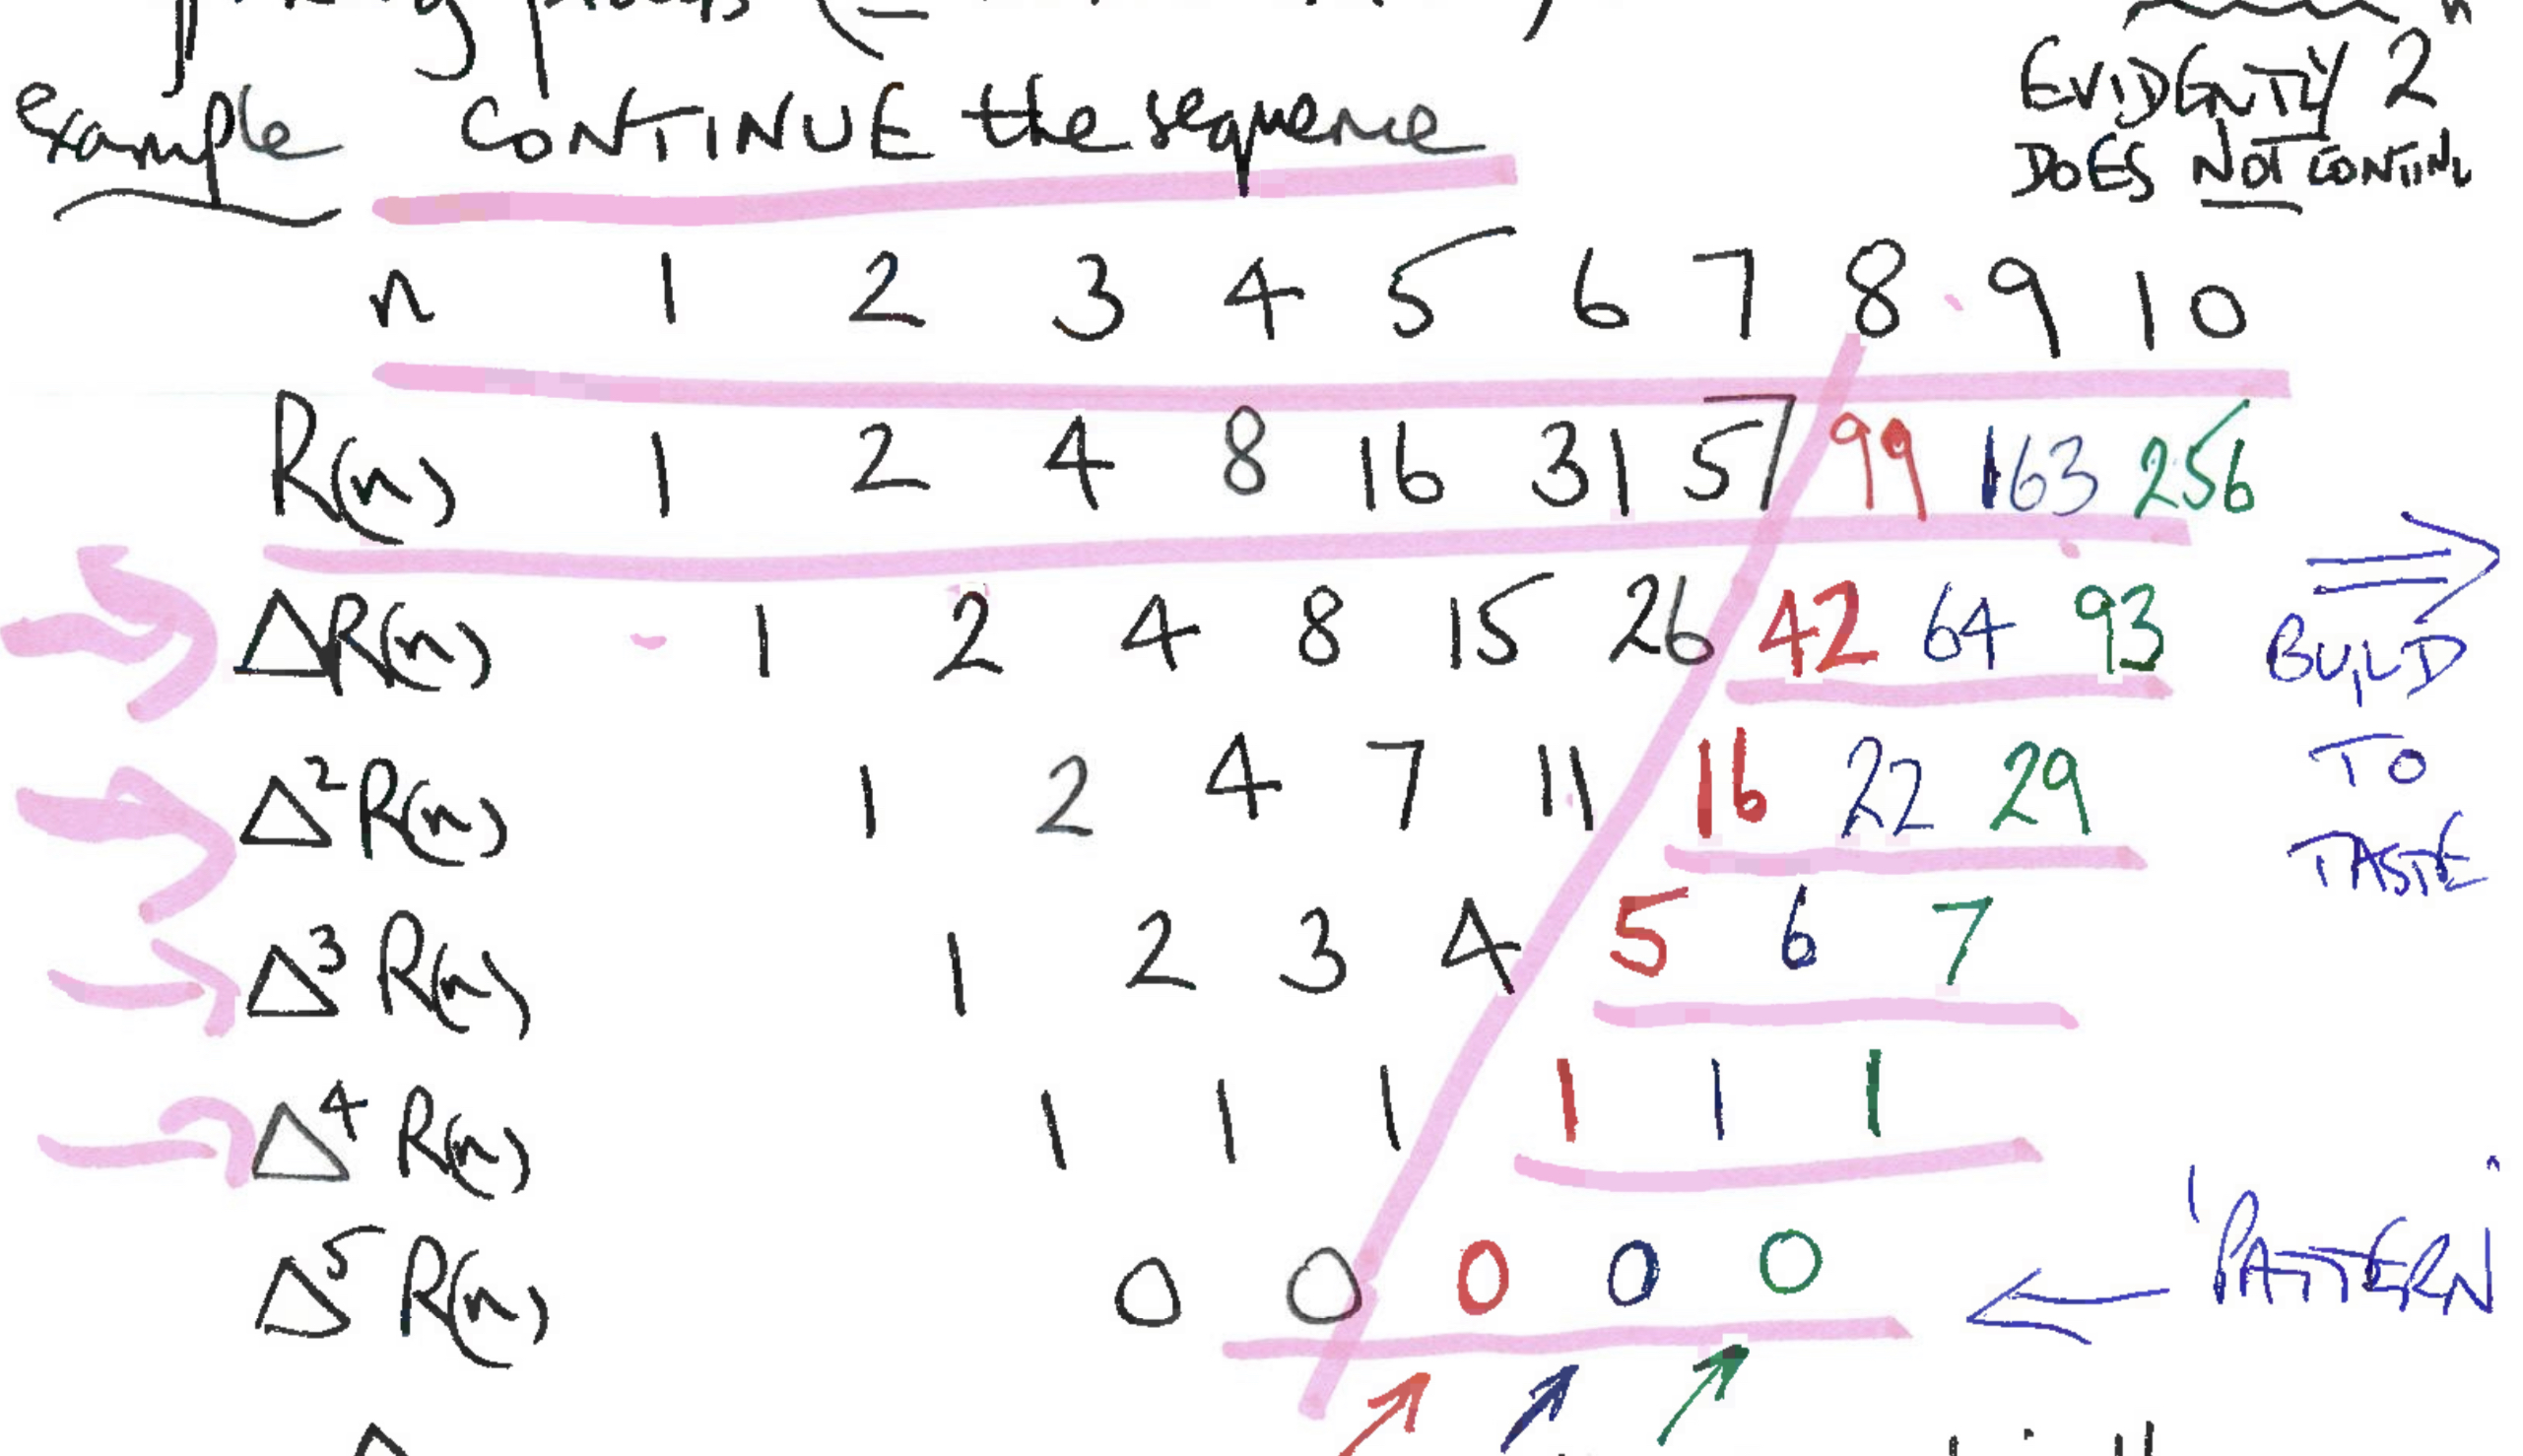
\includegraphics[scale = 0.15]{inverseDifferencing.jpg}
    \centering
    \caption{graph of reverse differencing porcess}\label{fig:invDiff}
    % In figure env, label is always after caption for it to function normally.
    \end{figure}
    
    \noindent And and example of the \emph{inverse} process is as shown in figure~\ref{fig:invDiff}.
    To find out the sequence of $R(n)$ beyond $n = 7$, one can keep on differencing
    the sequence (which is \emph{polynomial-like}) until its fourth and fifth order,
    realizing the repetitive $0$s and $1$s pattern, construct further 1s and 0s,
    and do the inverse back until order 0, i.e.\ constructing $R(n)$. 
    The pattern continues, in fact, only when $R(n)$ is a $k = 4$ degree polynomial in $n$.

    \medskip
    \noindent \underline{Note}: (Not in syllabus) There is a discrete analogy to Taylor's expansion,
    involving Newton's forward difference interpolation formula \ldots
\end{ex}

The sequence in the inverse process is actually\[
    \begin{align*} 
        & \begin{aligned}
        1 + (n - 1) + \frac{1}{2}(n-1)(n-2) & + \frac{1}{6}(n-1)(n-2)(n-3) \\
                                            & + \frac{1}{24}(n-1)(n-2)(n-3)(n-4) 
        \end{aligned} \\
                    & = \begin{pmatrix}
                            n-1 \\
                            0
                    \end{pmatrix} + \begin{pmatrix}
                            n-1 \\
                            1
                    \end{pmatrix} + \begin{pmatrix}
                            n-1 \\
                            2
                    \end{pmatrix} + \begin{pmatrix}
                            n-1 \\
                            3
                    \end{pmatrix} + \begin{pmatrix}
                            n-1 \\
                            4
                    \end{pmatrix} \\
                    & = \begin{pmatrix}
                            n \\
                            0
                    \end{pmatrix} + \begin{pmatrix}
                            n \\
                            2
                    \end{pmatrix} + \begin{pmatrix}
                            n \\
                            4
                    \end{pmatrix}.
    \end{align*}
\]
\begin{figure}
  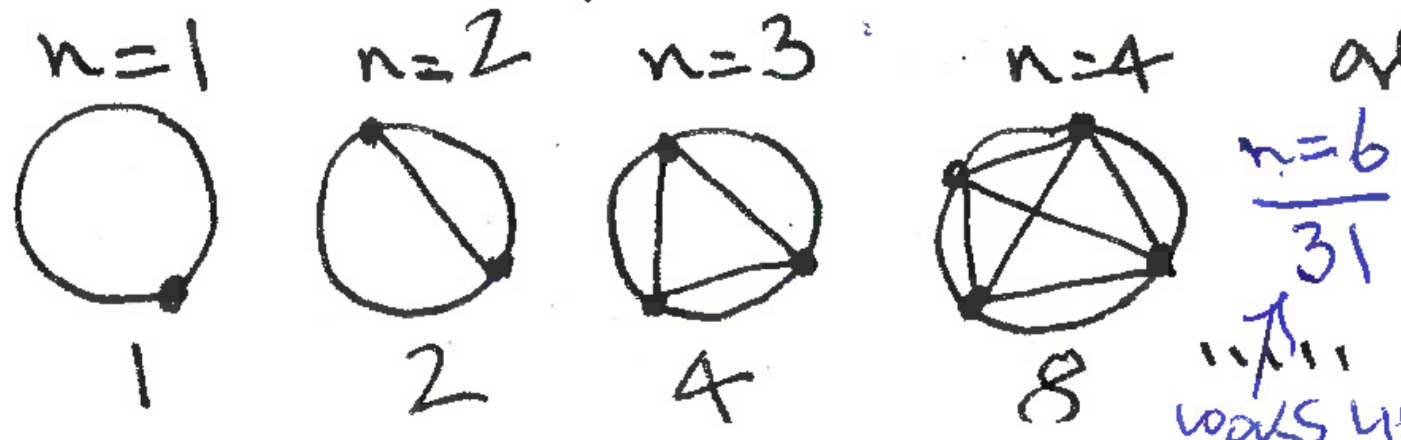
\includegraphics[scale=0.15]{circlePartition.jpeg}
  \centering
  \caption{Circle Division}\label{fig:circDiv}
\end{figure}

This expression represents the numbers of distinct regions into which the interior of a circle
is partitioned when $n$ distinct boundary points are connected by straight lines, as shown in figure~\ref{fig:circDiv}.
This is, however, not easy to prove!


\subsection{First Order Recurrence/Discrete Nonlinear Systems}

Consider $x_{n + 1} = F(x_n)$ where $x_n = x(n), x_n \neq 0$.
And we have initial choice $x_0$: \[
    \Rightarrow{} x_1 = F(x_0)
    \Rightarrow{} x_2 = F(x_1) = F(F(x_0)) = F^{(2)}(x_0) \Rightarrow{} \ldots
\]

This process is called \textbf{\emph{iteration}} ---
some function is used repeatedly --- \emph{iterative process}.
We can repersent this process graphically, as shown in Figure~\ref{fig:cobweb}.

\begin{figure}
  	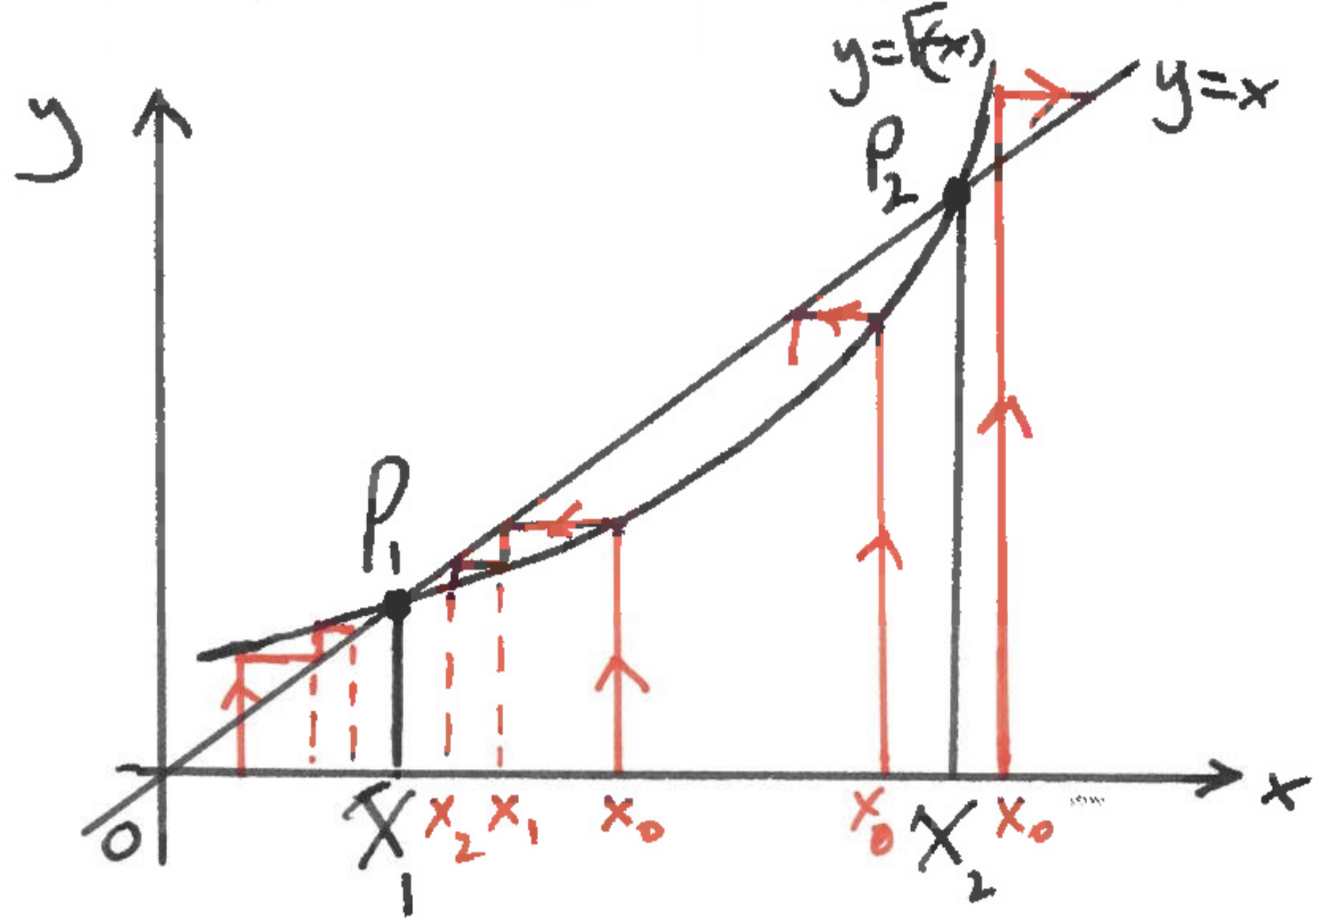
\includegraphics[scale=0.15]{CobwebDiagram.jpg}
  	\centering
    \caption{'Cobweb' Diagram}\label{fig:cobweb}
\end{figure}

There are 2 fixed points $P_1$ and $P_2$, for which the $x$ values satisfy\[
    X = F(X) \Rightarrow{} X_1, X_2.
\]
However, the \emph{character} of $P_1$ and $P_2$ is very different ---
initial values $x_0$ which start near $X_1$ have $x_n$ which approaches $X_1$,
while those $x_0$ which start near $X_2$ certainly are \emph{not} giving $x_n$
which approaches $X_2$!

\newmdtheoremenv[style=defEnv]{attractor and repeller}[theorem]{Definition}
\begin{attractor and repeller}
    $X_1$ corresponding to $P_1$ is said to be \textbf{\emph{asymptotically stable}} or \emph{attracting},
    and is called \textbf{\emph{attractor}};
    $X_2$ corresponding to $P_2$ is said to be \textbf{\emph{unstable}} or \emph{repelling},
    and is called \textbf{\emph{repeller}}.
\end{attractor and repeller}

How can we distinguish them analytically?

\medskip
Suppose $x_{n + 1} = F(x_n)$ and $X = F(X)$.
We put $X = x_n + \epsilon_n$ and imagine $x_0$ is chosen so that
$\epsilon_0$ is `small' i.e.\ $x_0$ is `near' to $X$.
Let's see how $\epsilon_n$ develops (whether $x_n$ converges or diverges to $X$):\[
        X - \epsilon_{n + 1} & = x_{n + 1} = F(x_n) = F(X - \epsilon_n)
        = F(X) - \epsilon_n F'(X) + \frac{1}{2}\epsilon_n^{2}F(X) + \cdots
        \]with the last step using taylor expansion, and by cancelling $X$ and $F(X)$, we get\[
        \epsilon_{n + 1} = \epsilon_n F'(X) - \frac{1}{2}\epsilon_n^{2}F''(X) + \cdots.
\]
$\epsilon_{n + 1}$ can therefore be estimated using different values of the various orders of $F(X)$:
\begin{itemize}
    \item $F'(X) \neq 0 \Rightarrow{} \epsilon_{n+1} \approx \epsilon_n F'(X)
        \Rightarrow{} \epsilon_n \approx \epsilon_0 {[F'(X)]}^{n}$.

        This process is called \textbf{\underline{first order process}}.
        Then if $|F'(X)|<1$, then $\epsilon_n \rightarrow{} 0$ and $X$ is an attractor.
        Otherwise if $|F'(X)|>1$, then $\epsilon_n$ diverges and $X$ is a repeller.
        However, if $|F'(X)| = 1$ then it depends on the case --- nothing is already proven.

    \item $F'(X) = 0, F''(X) \neq 0 \Rightarrow{} \epsilon \approx -\frac{1}{2}\epsilon_n^{2}F''(X)
        \Rightarrow{} \epsilon_{n + 1} \propto \epsilon_n^{2}$.

        This process is called \textbf{\underline{second order process}}.
        $\forall \epsilon_0$ sufficiently small, we have $\epsilon_n \rightarrow{} 0$,
        and $X$ is \emph{always} an attractor. 
        (Proof is not provided here.)
        
        Note that it is \emph{faster} than first order convergence,
        therefore it is usually preferred to design a process such that it is
        second order for studying that particular matter for better result.

    \item $F'(X) = 0, F''(X) = 0, F'''(X) \neq 0 \Rightarrow{} \epsilon_{n + 1} \propto \epsilon_n^{3}$.%chktex 23

        This process is called \textbf{\underline{third order process}}.
\end{itemize}
And so on. The \emph{rate} of convergence increases with the order of the process.
Third order process and beyond are usually unnecessary, but occasionally they
may be required. In practice we hope for second order,
but will often settle for first order.

\begin{ex}
    \,

    \begin{enumerate}[label = (\alph*)]
        \item \[
                x_{n+1} = \frac{1}{2}\left(x_n + \frac{A}{x_n}\right) = F(x_n)
        \]
        which is a method for finding $\sqrt{A}$.
        For instance, $A=12, x_0 = 2, \ldots, x_4 = 3.4641$, etc.

        The fixed points are $X = \frac{1}{2}\left(X + \frac{A}{X}\right)
        \rightarrow{} X = \pm \sqrt{A}$. By drawing the Cobweb diagram, we should see that
        $x_0 > 0 \Rightarrow{} x_n \rightarrow{} \sqrt{A}, x_0 < 0 \Rightarrow{} x_n \rightarrow{} \sqrt{A}$.

        Next we find out which order the process is:\[
            \begin{align*}
                F'(X)  & = \frac{1}{2}\left(1 - \frac{A}{X^{2}}\right) = 0 \\
                F''(X) & = \frac{A}{X^{3}} = \pm \frac{1}{\sqrt{A}} \neq 0.
            \end{align*}
        \]
        So this is a second order process, and $\pm \sqrt{A}$ are attractors with
        $\epsilon_{n + 1} \propto \epsilon_{n}^{2}$.

        \underline{Exercise}: Consider $A < 0$?

    \item Solve\[
            f(x) = x^{2} - 6x + 2 = 0.
    \]
    We can rearrange this in various ways and write it in iterative process:
    \begin{enumerate}[label = (\roman*)]
        \item $x_{n + 1} = 6 - \frac{2}{x}$
        \item $x_{n + 1} = \frac{1}{6}x_n^{2} + \frac{1}{3}$
        \item $x_{n + 1} = \sqrt{6x_n - 2}$
        \item $x_{n + 1} = x_n - \frac{x_n^{2} - 6x_n + 2}{2x - 6}
            = \frac{x_n^{2} - 2}{2x_n - 6}$.
    \end{enumerate}

    Examining these (see Problem Sheet 3) we find that (iv) is the `best buy'
    in that it is the \emph{only} second order process and it is the only one
    which allows us to obtain both roots and attractors if we choose $x_0$ suitably.

\item \[
        x_{n + 1} = x_n (2 - Ax_n)
\]
which is a method for finding a reciprocal \emph{without} division! ($x_n \rightarrow{} \frac{1}{A}$)
It is a second order process.

\underline{Note}: Examples (a), (b)(iv), (c) are examples of what is now called %chktex 36
the \emph{Newton(-Raphson) Method} for finding solutions of $f(x) = 0$: \[%chktex 36
    x_{n + 1} = F(x_n) = x_n - \frac{f(x_n)}{f'(x_n)}.
\]
Such a process is \emph{normally} at least second order (good!) because \[
    F'(x) = 1 - \frac{f'(x)}{f'(x)} + \frac{f(x)f''(x)}{{(f'(x))}^{2}} = 0
\]and\[
F''(x) = \frac{f''(x)}{f'(x)} \neq 0 \;\textnormal{usually}.
\]
However, there are some difficulties in implementing the method successfully,
including choosing a value near roots, having multiple roots, etc.
    
\item modern, practical, surprising\ldots \underline{Population Dynamics}

    Recall the \emph{logistic map equation}:\[
        P(n + 1) = aP(n) - b{(P(n))}^{2}
    \]
    which is a simple mathematical model with very complicated dynammics.
    Put $x_n = \frac{b}{a}P(n)$, and we get\[
        x_{n + 1} = ax_n(1 - x_n)
    \]
    with $a$ being the constant. This is the standard form of logistic map.

    Although there is no restriction for mathematical interest,
    the `physical' interest is in $0 \le a \le 4$ so that $[0, 1] \rightarrow{} [0, 1]$.
    We can easily see that the maximum value that $x_n (1 - x_n)$ can get is $\frac{1}{4}$,
    therefore having any $a > 4$ would definitely result in $x_{n + 1} > 1 \Rightarrow{}
    x_{n + 2} < 0$, and let alone $a < 0$.
    We certainly would not want negative population values!

    There are evidently two fixed points satisfying\[
        X = aX(1 - X) \Rightarrow{} X = 0 \;\textnormal{and}\; X = 1 - \frac{1}{a}.
    \]
    Which do we get, and when?
    Take the first order process and analyse with different ranges of $a$:\[
        |F'(X)| = |a(1 - 2X)|.
    \]
    \begin{itemize}
        \item $0 \le a < 1$, $a = 0$ is trivial.

            We can deduce that $x = 0$ is an attractor,
            while $x = 1 - \frac{1}{a}$ is a repeller.
            This makes sense because it is a linear model made worse by overcrowding.

        \item $1 < a < 3$.

            We can decude that $x= 0$ is a repeller,
            while $x = 1 - \frac{1}{a}$ is an attractor.
            This makes sense because it is an exponential growth stabilised by overcrowding.

            This behaviour is very similar to that of the logistic differential equation
            --- what follows is definitely not so!

        \item $a > 3$.

            We can deduce that $x = 0$ and $x = 1 - \frac{1}{a}$ are both repellers.

            So what exactly do we get?
            We get `\emph{period doubling}'.

            \medskip
            Consider $x_{n + 2} = F(x_{n + 1}) = F(F(x_{n})) = F^{(2)}(x_n)
            = a[ax_n (1 - x_n)][1 - ax_n(1 - x_n)]$.
            The fixed points of this satisfy
            \begin{equation}\label{eqn:1}
                X = a^{2}X(1 - X)[1 - aX(1-X)]
            \end{equation}
            We still have $X = 0, X = 1 - \frac{1}{a}$ of course,
            (it is a fixed point on a map done twice.)
            but now we have two new ones, say $X_1$ and $X_2$, satisfying
            \begin{equation}\label{eqn:2}
                a^{2}X^{2} - a(a+1)X + (a+1) = 0
            \end{equation}
            which is derived from dividing equation~\eqref{eqn:1} with the two known solutions.
            (Or do factorization accordingly.) 

            \medskip
            We also know that $X_1 = F(F(X_1)), X_2 = F(F(X_2))$.
            As such, choosing $X_1$, and applying the map once, we can see that $F(X_1) = F(F(F(X_1)))$,
            i.e.\ both $X_1$ and $F(X_1)$ are 
            \ul{the two fixed points of the map done twice},
            satisfying the equation~\eqref{eqn:2}, which is exactly looking for the two roots which are
            \ul{the fixed points of the logistic map done twice},
            and there are no other such fixed point except for $X_2$,
            thus we must have\[
                X_1 = F(X_2), \quad X_2 = F(X_1).
            \]

            This forms a \emph{flip} or \emph{2-cycle}. (Before becoming 4-cycle, 8-cycle, etc.)
            This is an attractor when\[
                \left|\frac{\mathrm{d}}{\mathrm{d}x} F(F(x)) \right| < 1
            \]\[
                \Rightarrow{} |F'(X_1)F'(X_2)| < 1,
                |a(1 - 2X_1) a(1 - 2X_2)| < 1
            \]and using Vieta's theorem to obtain the sum and product of the two roots
            from equation~\eqref{eqn:2}, we get\[
                3 < a < 1 + \sqrt{6}
            \]
            for positive $a$. For increasingly larger $a > 1 + \sqrt{6}$, we then obtain 4 cycle
            $\Rightarrow{}$ 8 cycle $\Rightarrow{} \ldots \Rightarrow{}$
            arbitrary number of cycle, or \emph{chaotic behaviour}!
    \end{itemize}
    \end{enumerate}
    
\end{ex}

\paragraph{Novelty!}
The stable windows (when it is still in a certain number of cycle instead of
being completely random, or rather \emph{chaotic} behaviour) get shorter in geometrical progression
at rate $\frac{1}{4.669\ldots}$, where $4.669\ldots$ is the \emph{Feigenbaum constant}.
(The first one. There is another one, which is not introduced by Berkshire, and 
actually beyond the scope of the current study, according to Wikipedia.)
For $3.57 < a \le 4$, `Chaos' + periodic windows!

\bigskip
For motivation to study this section, please watch the following youtube video:

\ul{https://www.youtube.com/watch?v=ovJcsL7vyrk}

\bigskip
For studying in detail, please read the following book recommended by our dear lecturer Frank Berkshire:

\ul{https://physicaeducator.files.wordpress.com/2018/02/classical-mechanics-by-kibble-and-berkshire.pdf}



\section{Linear Systems of Differential Equations}

\subsection{definitions and examples}

Previously we saw some simple examples of systems of differential equations,
where there is more than one dependent variable, e.g.\ the first order system
\begin{equation}\label{eqn:4}
    \left\{\begin{align*}
        & \frac{\mathrm{d}x}{\mathrm{d}t} = F(x,y) \\
        & \frac{\mathrm{d}y}{\mathrm{d}t} = G(x,y).
    \end{align*}\right.
\end{equation}
A very important class for us to consider is that of \emph{linear systems}:
\begin{equation}\label{eqn:3}
    \left\{\begin{align*}
        & \frac{\mathrm{d}x}{\mathrm{d}t} = ax + by \\
        & \frac{\mathrm{d}y}{\mathrm{d}t} = cx + dy
    \end{align*}\right.
\end{equation}
where, in general, $a, b, c, d$ could be functions of time ---
we take them to be \emph{constants} in our discussion.
System~\eqref{eqn:3} is called \textbf{\emph{homogeneous}}.
If there are further \underline{added} constants or functions of time
on RHS of~\eqref{eqn:3} then the system would be called \textbf{\emph{inhomogeneous}}.

\noindent \underline{Notes}:~\eqref{eqn:3} is a \textbf{\emph{coupled system}} in general,
in that $x$ and $y$ appear on \emph{each} RHS.\@

\paragraph{Examples}
\,

\begin{enumerate}[label = (\alph*)]
    \item \underline{Combat}:\[
        \left\{\begin{align*}
            & \frac{\mathrm{d}x}{\mathrm{d}t} = -ay \\
            & \frac{\mathrm{d}y}{\mathrm{d}t} = -bx.
        \end{align*}\right.
    \]
    Here $a = 0 = d$; $b, c$ are both negative in~\eqref{eqn:3}.

\item \underline{Romance}!\[
    \left\{
        \begin{align*}
            & \frac{\mathrm{d}r}{\mathrm{d}t} = ar + bj \\
            & \frac{\mathrm{d}j}{\mathrm{d}t} = cr + dj
        \end{align*}
        \right.
\]
where $a,b,c,d$ can plausibly be positive or negative!
($r(t)$ is Romeo's love/hate for Juliet at time $t$.
Similarly, $j(t)$ is Juliet's love/hate for Romeo at time $t$.)

\item \underline{Linear Ordinary Differential Equations of higher order}

    E.g.\ Our damped harmonic oscillator\[
        \frac{\mathrm{d}^{2}x}{\mathrm{d}t^{2}} + 2k\frac{\mathrm{d}x}{\mathrm{d}t}
        + \omega^{2}x = 0
    \]can be written in the form
    \begin{equation}\label{eqn:7}
        \left\{
            \begin{align*}
                & \frac{\mathrm{d}x}{\mathrm{d}t} = y \\
                & \frac{\mathrm{d}y}{\mathrm{d}t} = \omega^{2}x - 2ky.
            \end{align*}
            \right.
    \end{equation}

\item \underline{General nonlinear systems}

    In general we can find equilibria of~\eqref{eqn:4} by solving
    $F(x,y) = 0 = G(x,y)$. The local behaviour of $x,y$ near these equilibria
    is that of a local linear System (via Taylor expansion).
    This analysis allows us to infer the properties of the full nonlinear systems.
\end{enumerate}

How do we solve \emph{linear systems} like~\eqref{eqn:3}?

A desirable and worthy aim is to try to \emph{decouple} the equations ---
if necessary by making a suitable change of variables. This is a good idea
because if we have a decoupled system, e.g.\[
    \frac{\mathrm{d}x}{\mathrm{d}t} = 2x, \quad \frac{\mathrm{d}y}{\mathrm{d}t} = -3y
\]then for an initial ($t = 0$) point $(x_0, y_0)$ the solution would be
$(x,y) = (x_0 e^{2t}, y_0 e^{-3t})$. In this case, as shown in Figure~\ref{fig:phasePortrait},
all the trajectories are given by
$x^{3}y^{2} =$ constant, and the particular solution has $x^{3}y^{2} = x_0^{3}y_0^{2}$.
Within a family of solutions, the value of $x$ and $y$ changes as the value of $t$ changes,
with the direction specified in the diagram. 

As such, we can also see that there is one equilibrium point at $O(0, 0)$, where any changes
in the value of $t$ does not change the value of $x$ and $y$. In addition, the equilibrium point
is \emph{not stable} since, although having perturbation in the $y$-axis converges back to 0,
perturbations along the $x$-axis diverges to infinity. So $O$ is definitely not an attractor.

\begin{figure}
  	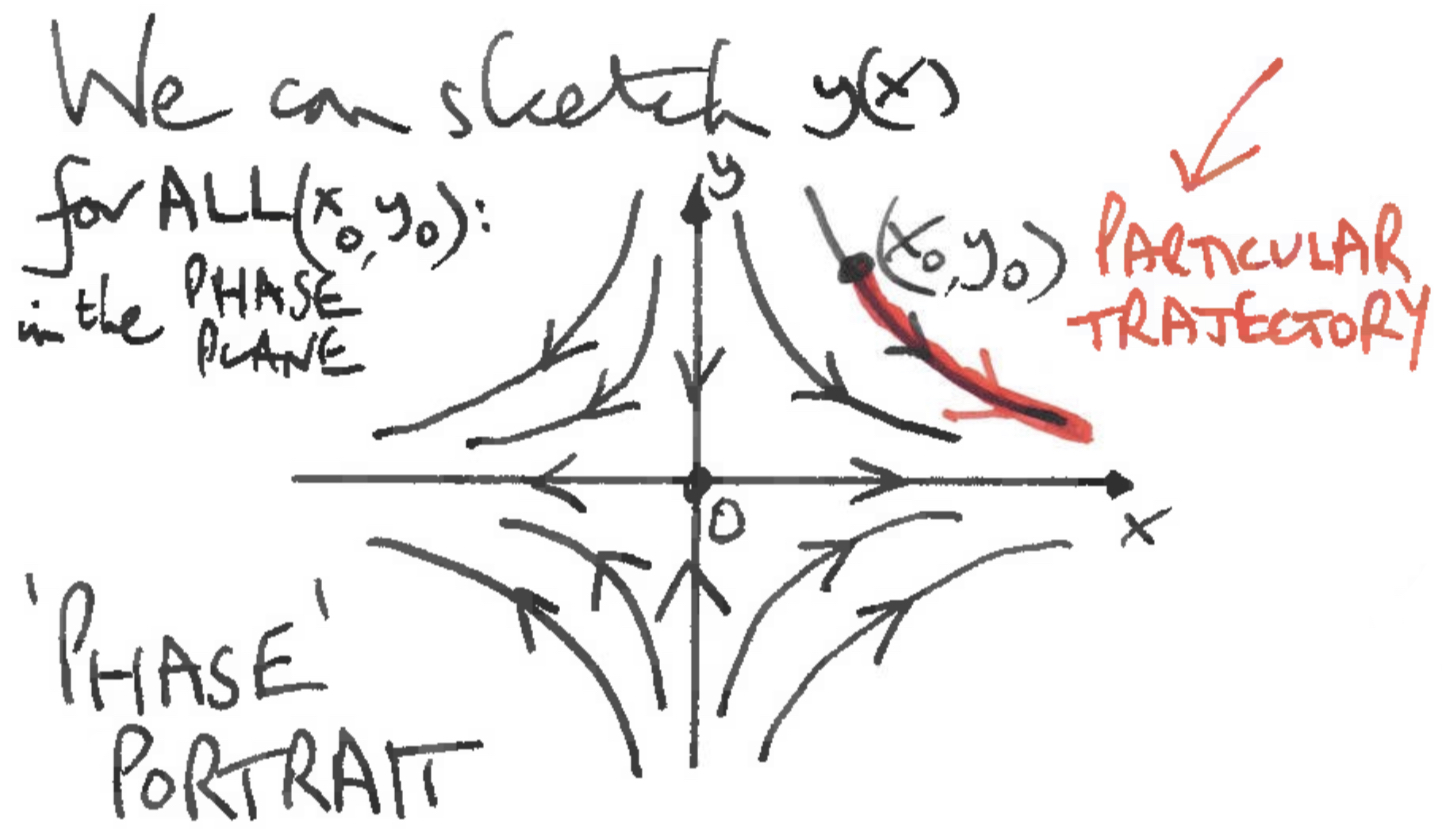
\includegraphics[scale=0.15]{phasePortrait.jpeg}
  	\centering
    \caption{`phase' portrait}\label{fig:phasePortrait}
\end{figure}

\bigskip
What can be done with a coupled system? e.g.
\begin{equation}\label{eqn:5}
    \left\{
        \begin{align*}
            & \frac{\mathrm{d}x}{\mathrm{d}t} = -4x - 3y \\
            & \frac{\mathrm{d}y}{\mathrm{d}t} = 2x + 3y
        \end{align*}\right.
\end{equation}

(For the moment we consider a homogeneous system --- some inhomogeneous later.)

\paragraph{Methods}
\;

\begin{enumerate}[label = (\arabic*)]
    \item We might recognize that \[
            \left(\frac{\mathrm{d}}{\mathrm{d}t} + 4\right) x = -3y \quad\textnormal{and}\quad
            \left(\frac{\mathrm{d}}{\mathrm{d}t} - 3\right) y = 2x
    \]\[
    \Rightarrow{} \left(\frac{\mathrm{d}}{\mathrm{d}t} - 3\right) 
    \left(\frac{\mathrm{d}}{\mathrm{d}t} + 4\right) x
    = -3\left(\frac{\mathrm{d}}{\mathrm{d}t} - 3\right) y = -6x
    \]\[
        \Rightarrow{}\frac{\mathrm{d}^{2}x}{\mathrm{d}t^{2}} + \frac{\mathrm{d}x}{\mathrm{d}t} - 6x = 0.
    \]
    Solve this using the previous methods: $\lambda_1 = 2, \lambda_2 = -3$, so that
    $x(t) = A_1e^{2t} + A_2e^{-3t}$. Naturally we can then find $y(t)$ from the first rearrangement above:\[
        y(t) = -\frac{1}{3}\left(\frac{\mathrm{d}}{\mathrm{d}t} + 4\right) x
        = -2A_1e^{2t} - \frac{1}{3}A_2e^{-3t}
    \]and we note that our solution for $x(t), y(t)$ depends on 2 arbitrary constants --- as it must!

    Afterwards, we can also find $y(x)$ by eliminating $t$, if we wish. Using the expressions we obtained
    for $x(t)$ and $y(t)$, we can obtain \[
        (x + 3y) = -5A_1e^{2t}, \quad (2x + y) = \frac{5}{3}A_2e^{-3t}
    \]\[
    \Rightarrow{} {(x + 3y)}^{3} {(2x + y)}^{2} = \frac{3125}{9}A_1^{3}A_2^{2}.
    \]
    We can then draw the family of trajectories in the $(x,y)$ plane (phase portrait).

\item We might also note that our~\eqref{eqn:5} can be written as\[
    \frac{\mathrm{d}y}{\mathrm{d}x} = \frac{\frac{\mathrm{d}y}{\mathrm{d}t} }{\frac{\mathrm{d}x}{\mathrm{d}t} }
    = \frac{2x + 3y}{-4x - 3y} = \frac{2 + 3 \left(\frac{y}{x}\right) }{-4 - 3 \left(\frac{y}{x}\right) }.
\]
This is homogeneous 1st order D.E. We put $\frac{y}{x} = u(x) \Rightarrow{} x\frac{\mathrm{d}u}{\mathrm{d}x} 
+ u = \frac{2 + 3u}{-4 - 3u}$, and then we get\[
    x\frac{\mathrm{d}u}{\mathrm{d}x} = \frac{2 + 7u + 3u^{2}}{-4 - 3u}
\]solving this equation and we get\[
    -\ln{x} = \frac{3}{5}\ln{(1 + 3u)} + \frac{2}{5}\ln{(2 + u)} + C
\]substituting $x$ and $y$ back and eliminating $t$ and we get\[
{(x + 3y)}^{3}{(2x + y)}^{2} = C.
\]

\underline{Warning}: This method is not favourable as it does not contain any information regarding $t$--- 
it was got rid of at the very start, therefore no time-depence of $x$ and $y$, i.e.\ $x(t), y(t)$.
As a result, we cannot do certain things such as drawing the phase portrait!

\item We might just \emph{\underline{notice(!)}} that\[ %chktex 36
    \begin{align*}
        & \frac{\mathrm{d}}{\mathrm{d}t} (2x + y) = 2(-4x - 3y) + (2x + 3y) = -3(2x + y) \\
        & \frac{\mathrm{d}}{\mathrm{d}t} (x + 3y) = (-4x - 3y) + 3(2x + 3y) = 2(x + 3y)
    \end{align*}
\]so that\[
    \left\{
        \begin{align*}
            2x + y & = C_1e^{-3t} \\
            x + 3y & = C_2e^{2t}
        \end{align*}
        \right.
\]\[
    \Rightarrow{}\left\{
        \begin{align*}
            x & = \frac{3}{5}C_1e^{-3t} - \frac{1}{5}C_2e^{2t} \\
            y & = -\frac{1}{5}C_1e^{-3t} + \frac{2}{5}C_2e^{2t}
        \end{align*}
        \right.
    \]and of course ${(x + 3y)}^{3}{(2x + y)}^{2} = C$ again.
    \begin{figure}
      	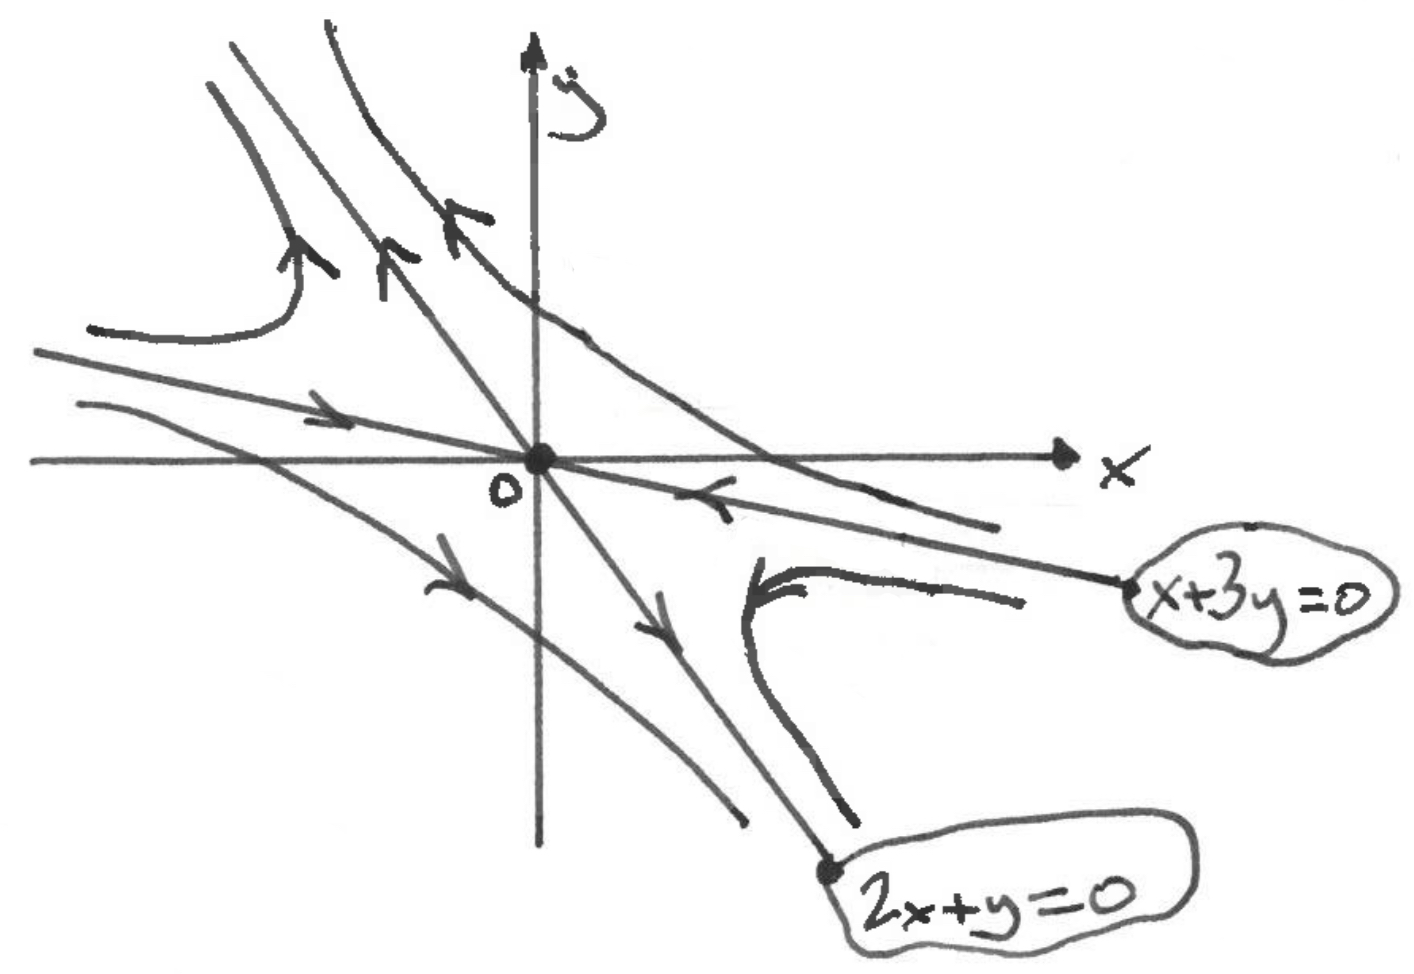
\includegraphics[scale=0.15]{2ndPhasePortrait.jpeg}
      	\centering
        \caption{phase portrait of~\eqref{eqn:5}}\label{fig:2ndPhaseP}
    \end{figure}
    

    All the aforementioned methods have the same phase portrait, as shown in Figure~\ref{fig:2ndPhaseP}.
    The direction of the two straight lines $x + 3y = 0$ and $2x + y = 0$ can be found easily,
    and the other four trajectories has to follow the same direction as those two straight lines,
    unless there are two trajectories intersect and have an equilibrium point.

    Method (3) gives the germ of a good idea!

\item How can we arrive at the linear combinations we used previously in an orderly manner
    and not just `by inspection' or luck?!

    We write our system~\eqref{eqn:5} in a different way:
    \begin{equation}\label{eqn:6}
        \frac{\mathrm{d}}{\mathrm{d}t} \begin{pmatrix}
                x \\
                y
        \end{pmatrix} = \begin{pmatrix}
        -4 & -3 \\
        2 & 3
        \end{pmatrix} \begin{pmatrix}
                x \\
                y
        \end{pmatrix} 
    \end{equation}
      which is $\frac{\mathrm{d}}{\mathrm{d}t} \mathbf{v} = M\mathbf{v}$ in vector/matrix notation.
      Now try $\mathbf{v} = \mathbf{V}e^{\lambda t}$ with $\mathbf{V}$ \emph{not} depending on $t$,
      i.e.\ it is a \emph{constant vector}. This implies that\[
          M\mathbf{V} = \lambda \mathbf{V}, \;\textnormal{i.e.}\; (M - \lambda I)\mathbf{V} = \mathbf{0}
      \]converting to an eigenvalue/eigenvector problem to find appropriate $\lambda, \mathbf{V}$.

      For non-trivial $\mathbf{V}$ (i.e.\ $\neq 0$) then we must have\[
          \det{
          \begin{pmatrix}
              -4-\lambda & -3 \\
              2 & 3-\lambda
          \end{pmatrix} 
      } = 0
      \]
      $\Rightarrow{}(-4-\lambda)(3-\lambda)+6 = 0$, $\lambda^{2}+\lambda-6 = 0$,
      $\lambda_1 = 2, \lambda_2 = -3$.
      And computing the respective eigenvector, we get
      \[\mathbf{V}_1 = \begin{pmatrix}
              1 \\
              -2
      \end{pmatrix} , \mathbf{V}_2 = \begin{pmatrix}
              3 \\
              -1
          \end{pmatrix} ,\] or any scalar multiple of these vectors.
      (Substitute $\lambda_1, \lambda_2$ into $(M - \lambda I)$ and compute its RRE,
      and read off from RRE.)

      We now note the \emph{linearity} of our system, so we can write\[
          \begin{pmatrix}
                  x \\
                  y
          \end{pmatrix} = B_1\begin{pmatrix}
                  1 \\
                  -2
          \end{pmatrix} e^{2t} + B_2\begin{pmatrix}
                  3 \\
                  -1
          \end{pmatrix} e^{-3t}
      \]where $B_1, B_2$ are arbitrary constants.
      Therefore $x = B_1 e^{2t} + 3B_2 e^{-3t}$,
      $y = -2B_{1}e^{2t} - B_2 e^{-3t}$.
      (Note: results are the same as the previous methods.)
\end{enumerate}

\subsection{System decoupling}
How does the last method do it? From the eigenvectors $\mathbf{V}_1, \mathbf{V}_2$ form the matrix\[
    S = (\mathbf{V}_1 \quad \mathbf{V}_2) \qquad\textnormal{i.e.\ 2 $\times$ 2}
\]and write \[\mathbf{v} = \begin{pmatrix}
        x \\
        y
    \end{pmatrix} = S\begin{pmatrix}
            \xi \\
            \eta
    \end{pmatrix}.
\](\emph{Similarity transformation}: tranform linearly $(x,y)$ to new axes $(\xi, \eta)$)
The vector form of~\eqref{eqn:6} becomes\[
    \frac{\mathrm{d}}{\mathrm{d}t} \left[S \begin{pmatrix}
            \xi \\
            \eta
    \end{pmatrix} \right] 
    = S\frac{\mathrm{d}}{\mathrm{d}t} \begin{pmatrix}
            \xi \\
            \eta
    \end{pmatrix} 
    = MS\begin{pmatrix}
            \xi \\
            \eta
    \end{pmatrix} 
\]\[
    \Rightarrow{}\frac{\mathrm{d}}{\mathrm{d}t} \begin{pmatrix}
            \xi \\
            \eta
    \end{pmatrix} = S^{-1}MS\begin{pmatrix}
            \xi \\
            \eta
    \end{pmatrix} 
\]assuming that $S$ is a \emph{nonsingular matrix} (invertible).  
Then by noting that\[
    S^{-1}S = \begin{pmatrix}
            R_1 \\
            R_2
    \end{pmatrix} \begin{pmatrix}
    \mathbf{V}_1 & \mathbf{V}_2
    \end{pmatrix} = I_n
\]where $R_1, R_2$ are of dimension $1 \times 2$.
Using $M\mathbf{V} = \lambda \mathbf{V}$, we can deduce that\[
    S^{-1}MS = \begin{pmatrix}
            R_1 \\
            R_2
    \end{pmatrix} MS = \begin{pmatrix}
            R_1 \\
            R_2
    \end{pmatrix} \begin{pmatrix}
    \lambda_1 \mathbf{V}_1 & \lambda_2 \mathbf{V}_2
    \end{pmatrix} = \begin{pmatrix}
    \lambda_1 & 0 \\
    0 & \lambda_2
    \end{pmatrix} 
\]which is a diagonal matrix. 
For instance, in~\eqref{eqn:6}, \[
    S = \begin{pmatrix}
        1 & 3 \\
        -2 & -1
    \end{pmatrix}, S^{-1} = \frac{1}{5} \begin{pmatrix}
        -1 & -3 \\
        2 & 1
    \end{pmatrix} 
\]\[
    \Rightarrow{}\frac{\mathrm{d}}{\mathrm{d}t} \begin{pmatrix}
            \xi \\
            \eta
    \end{pmatrix} = \begin{pmatrix}
    2 & 0 \\
    0 & -3
    \end{pmatrix} \begin{pmatrix}
            \xi \\
            \eta
    \end{pmatrix}
\]and this is decoupled!
As such, $\frac{\mathrm{d}}{\mathrm{d}t} \xi = 2\xi, \frac{\mathrm{d}}{\mathrm{d}t} \eta = -3\eta$
$\Rightarrow{}\xi = C_1 e^{2t}, \eta = C_2 e^{-3t}$. Therefore as before, \[
    \begin{pmatrix}
            x \\
            y
    \end{pmatrix}  = S\begin{pmatrix}
            \xi \\
            \eta
    \end{pmatrix} = \begin{pmatrix}
            C_1 e^{2t} + 3C_2 e^{-3t} \\
            -2C_1 e^{2t} - C_2 e^{-3t}
    \end{pmatrix} 
\]

\paragraph{General Theory}
Does this vector/matrix method always work?

For $\mathbf{v} = \begin{pmatrix}
        x \\
        y
\end{pmatrix} , \frac{\mathrm{d}\mathbf{v}}{\mathrm{d}t} = M\mathbf{v}$,
substituting with $\mathbf{v} = \mathbf{V}e^{\lambda t}$,
we get $(M - \lambda I)\mathbf{V} = \mathbf{0}$.
The solution depends \emph{crucially} on the nature of the eigenvalue/eigenvector problem
$\lambda_1, \mathbf{V}_1, \lambda_2, \mathbf{V}_2$.

We note that $\lambda_1 + \lambda_2 =$ \emph{trace} of $M$ (sum of the leading diagonal of $M$),
and $\lambda_1\lambda_2 = \det{M}$. Both can be derived by looking at the quadratic equation
derived from calculating the determinant of $(M - \lambda I)$ to be $0$.
The equation is \emph{characteristic} for $M$.
\begin{itemize}
        \item $\lambda_1 \neq \lambda_2$

            Our example~\eqref{eqn:6} was of this type, thereby having
            $\mathbf{V}_1, \mathbf{V}_2$ eigenvectors. Our system decouples via 
            the \emph{similarity transformation} and $S^{-1}MS$ is a diagonal matrix.  
            This is essentially the situation even when the $\lambda_i$ are \emph{complex}.

        \item $\lambda_1 = \lambda_2 = \lambda$

            We've always had some difficulty with the equal roots cases\ldots
            Here the difficulty presents in that the matrix $S$, which effects
            the desired decoupling \emph{may not exist}.

            \begin{enumerate}[label = (\roman*)]
                \item 2 distinct eigenvectors exist.
                    
                    If $\mathbf{V}_1, \mathbf{V}_2$ are distinct for $M, \lambda$
                    then it is true that $M\mathbf{v} = \lambda\mathbf{v}$ for any vector,
                    i.e.\ $M = \lambda I$ and\[
                        \begin{pmatrix}
                                x \\
                                y
                        \end{pmatrix} = B_1 \mathbf{V}_1 e^{\lambda t} + B_2 \mathbf{V}_2 e^{\lambda t}.
                    \]
                    with $\mathbf{V}_1, \mathbf{V}_2$ being two linearly-independent 
                    and random vectors in the plane.

                \item Only one eigenvector exists.

                    The best that can be done by a similarity transformation
                    is to reduce the system to e.g.\[
                        \frac{\mathrm{d}}{\mathrm{d}t} \begin{pmatrix}
                                \xi \\
                                \eta
                        \end{pmatrix} = \begin{pmatrix}
                        \lambda & 0 \\
                        1 & \lambda
                        \end{pmatrix} \begin{pmatrix}
                                \xi \\
                                \eta
                        \end{pmatrix}
                    \]or equivalent. The diagonal form is \emph{not} achievable. 
                    By looking at $\frac{\mathrm{d}\eta}{\mathrm{d}t} $, we realize that\[
                        \frac{\mathrm{d}\eta}{\mathrm{d}t} = \xi + \lambda \eta
                        \Rightarrow{}\frac{\mathrm{d}\eta}{\mathrm{d}t} - \lambda \eta = \xi,
                    \]
                    where the CF of $\eta$ already appears in $\xi$.
                    So we have to use $t e^{\lambda t}$ instead. As such,\[
                        \begin{pmatrix}
                                \xi \\
                                \eta
                        \end{pmatrix} = C_1 \begin{pmatrix}
                                0 \\
                                1
                        \end{pmatrix} e^{\lambda t} + C_2 \begin{pmatrix}
                                1 \\
                                t
                        \end{pmatrix} e^{\lambda t}.
                    \]
            \end{enumerate}
\end{itemize}

\underline{Note}: If $M$ is actually a \emph{symmetric matrix} with real entries then
$\lambda_1, \lambda_2$ are real, the $\mathbf{V}_1, \mathbf{V}_2$ are real and orthogonal.
If we then choose $\mathbf{V}_1, \mathbf{V}_2$ (as we may, if we wish) to be of unit length (normalised),
then $S^{-1} = S^{T}$ and $S$ represents a rotation in the $x, y$ plane (or rotation + reflection).
$S$ is an orthogonal matrix.

\subsection{Typical Phase Portraits}

What do the phase portraits look like in the various different cases?
The eigenvalues $\lambda_1, \lambda_2$ are evidently crucial in determining the structure
and the time $t$ evolution arrows on the trajectories.

The eigenvectors determine the crucial $\xi, \eta$ decoupled coordinate directions,
where appropriate. We note in the interpretation of the diagrams that\[
    \xi \propto e^{\lambda_1 t},\quad \eta \propto e^{\lambda_2 t}
\]\[
\Rightarrow{}\xi \propto \eta^{\frac{\lambda_1}{\lambda_2}},\quad
\frac{\mathrm{d}\xi}{\mathrm{d}\eta} \propto \eta^{\frac{\lambda_1}{\lambda_2} - 1}
\;\textnormal{in general}.
\]
Thus dominant eigenvector \emph{nearly always} depends on 
$\left|\frac{\lambda_1}{\lambda_2}\right| > 1$ or $\left|\frac{\lambda_1}{\lambda_2}\right| < 1$,
and the other trajectories come in \emph{parallel}/\emph{tangent} to the dominant eigenvector.  
Now pardon me for the shameleses numerous screenshots of Berkshire's notes for the phase portraits.

\begin{figure}
  	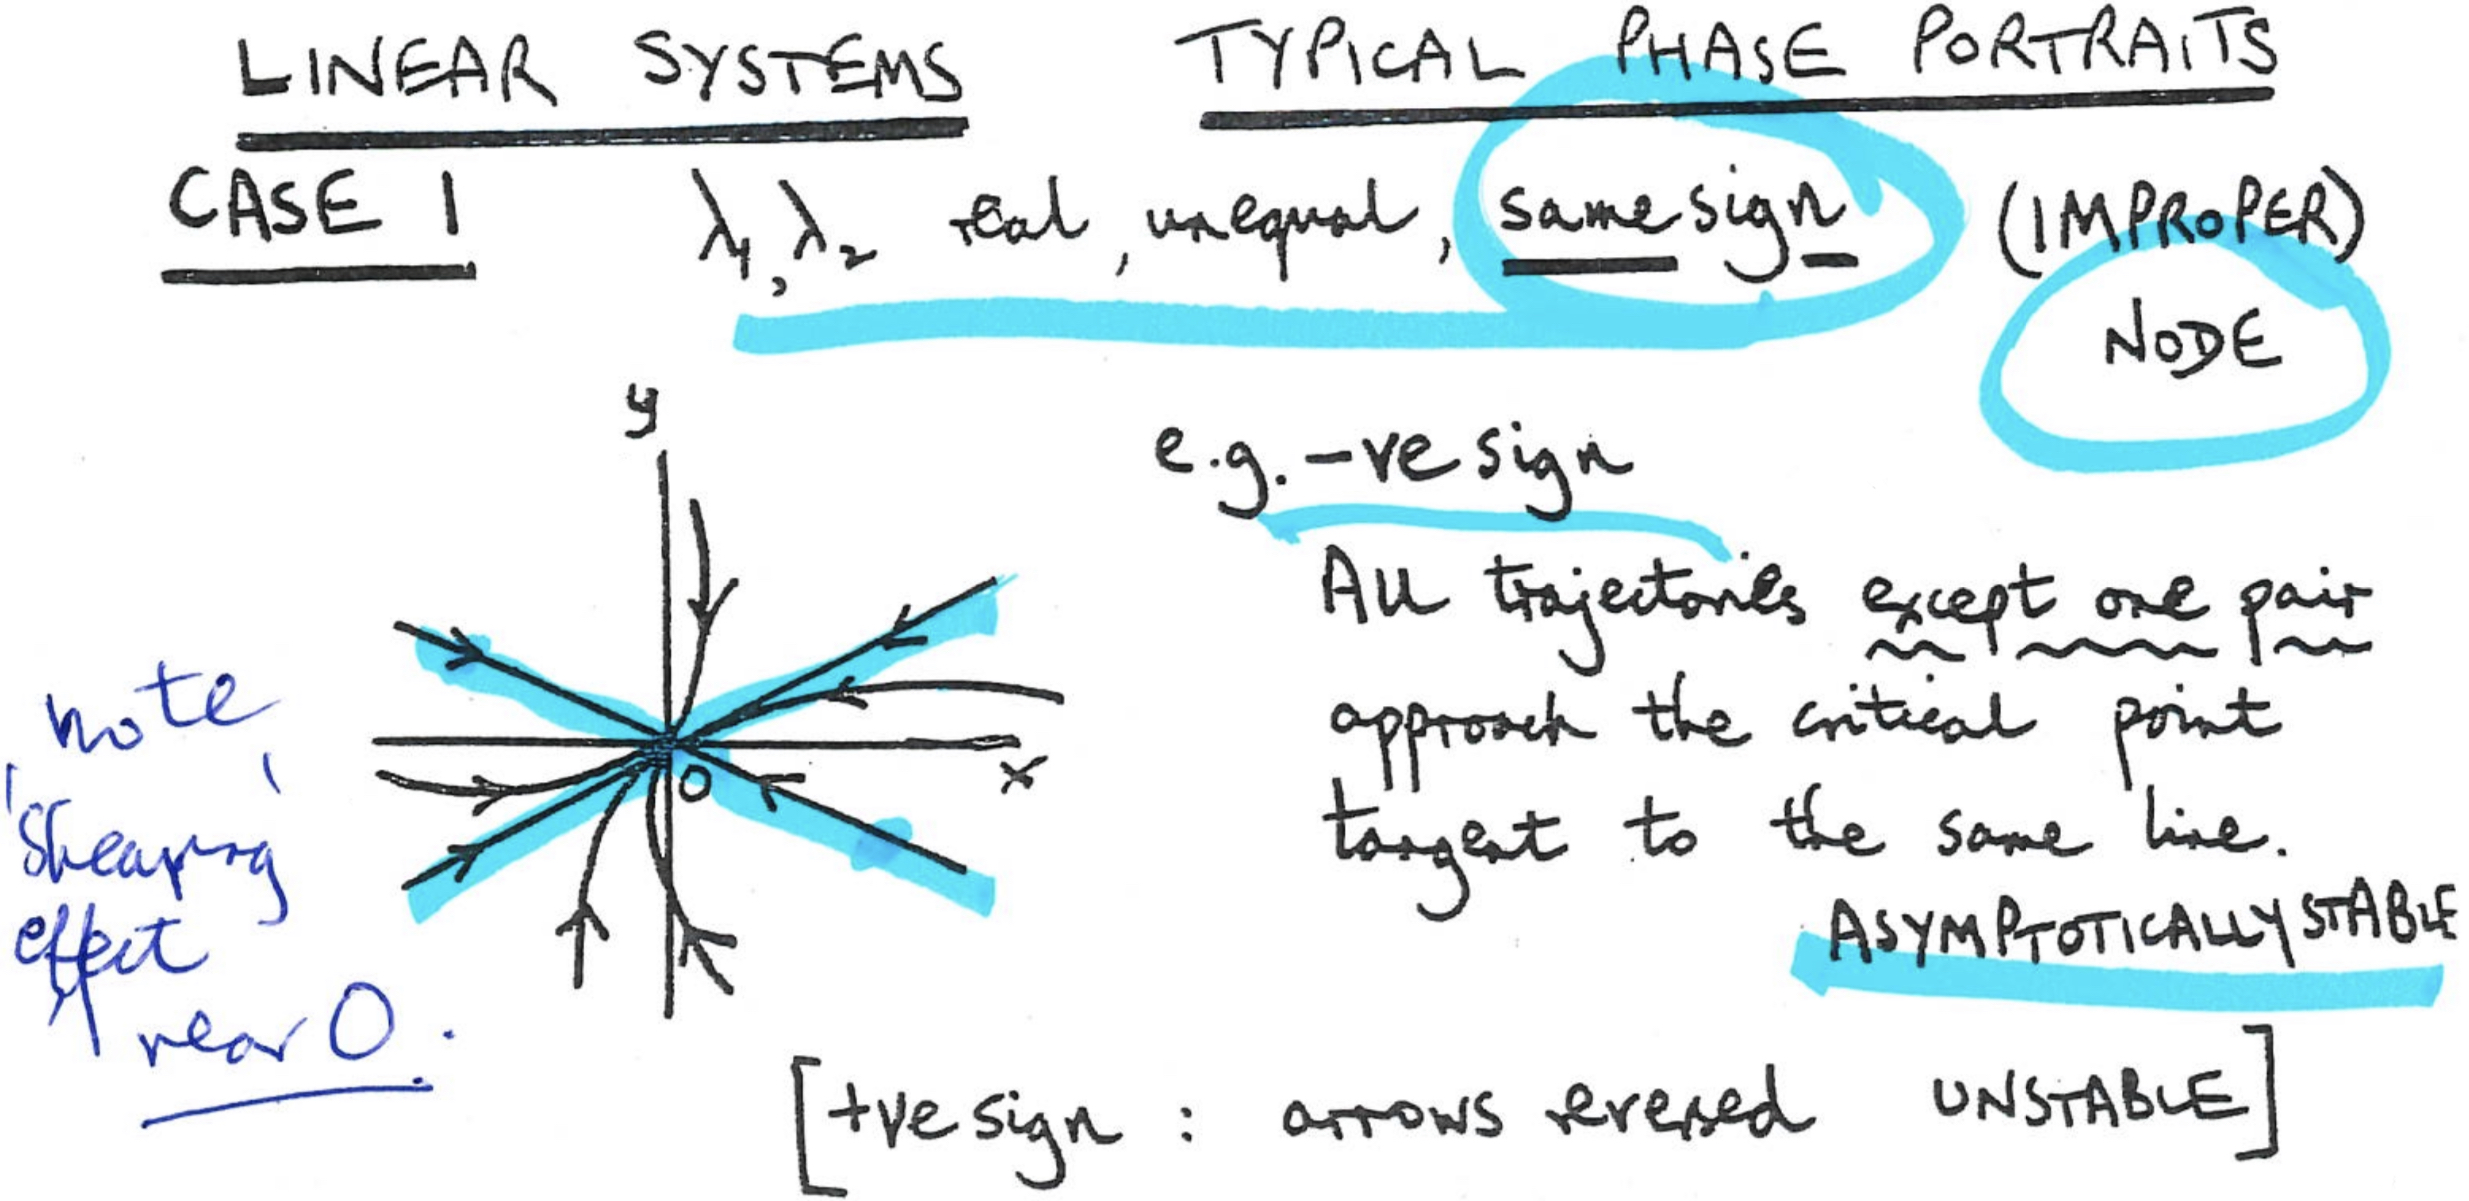
\includegraphics[scale=0.15]{PP1.jpeg}
  	\centering
  	\caption{case 1}\label{PP1}
\end{figure}

\begin{figure}
  	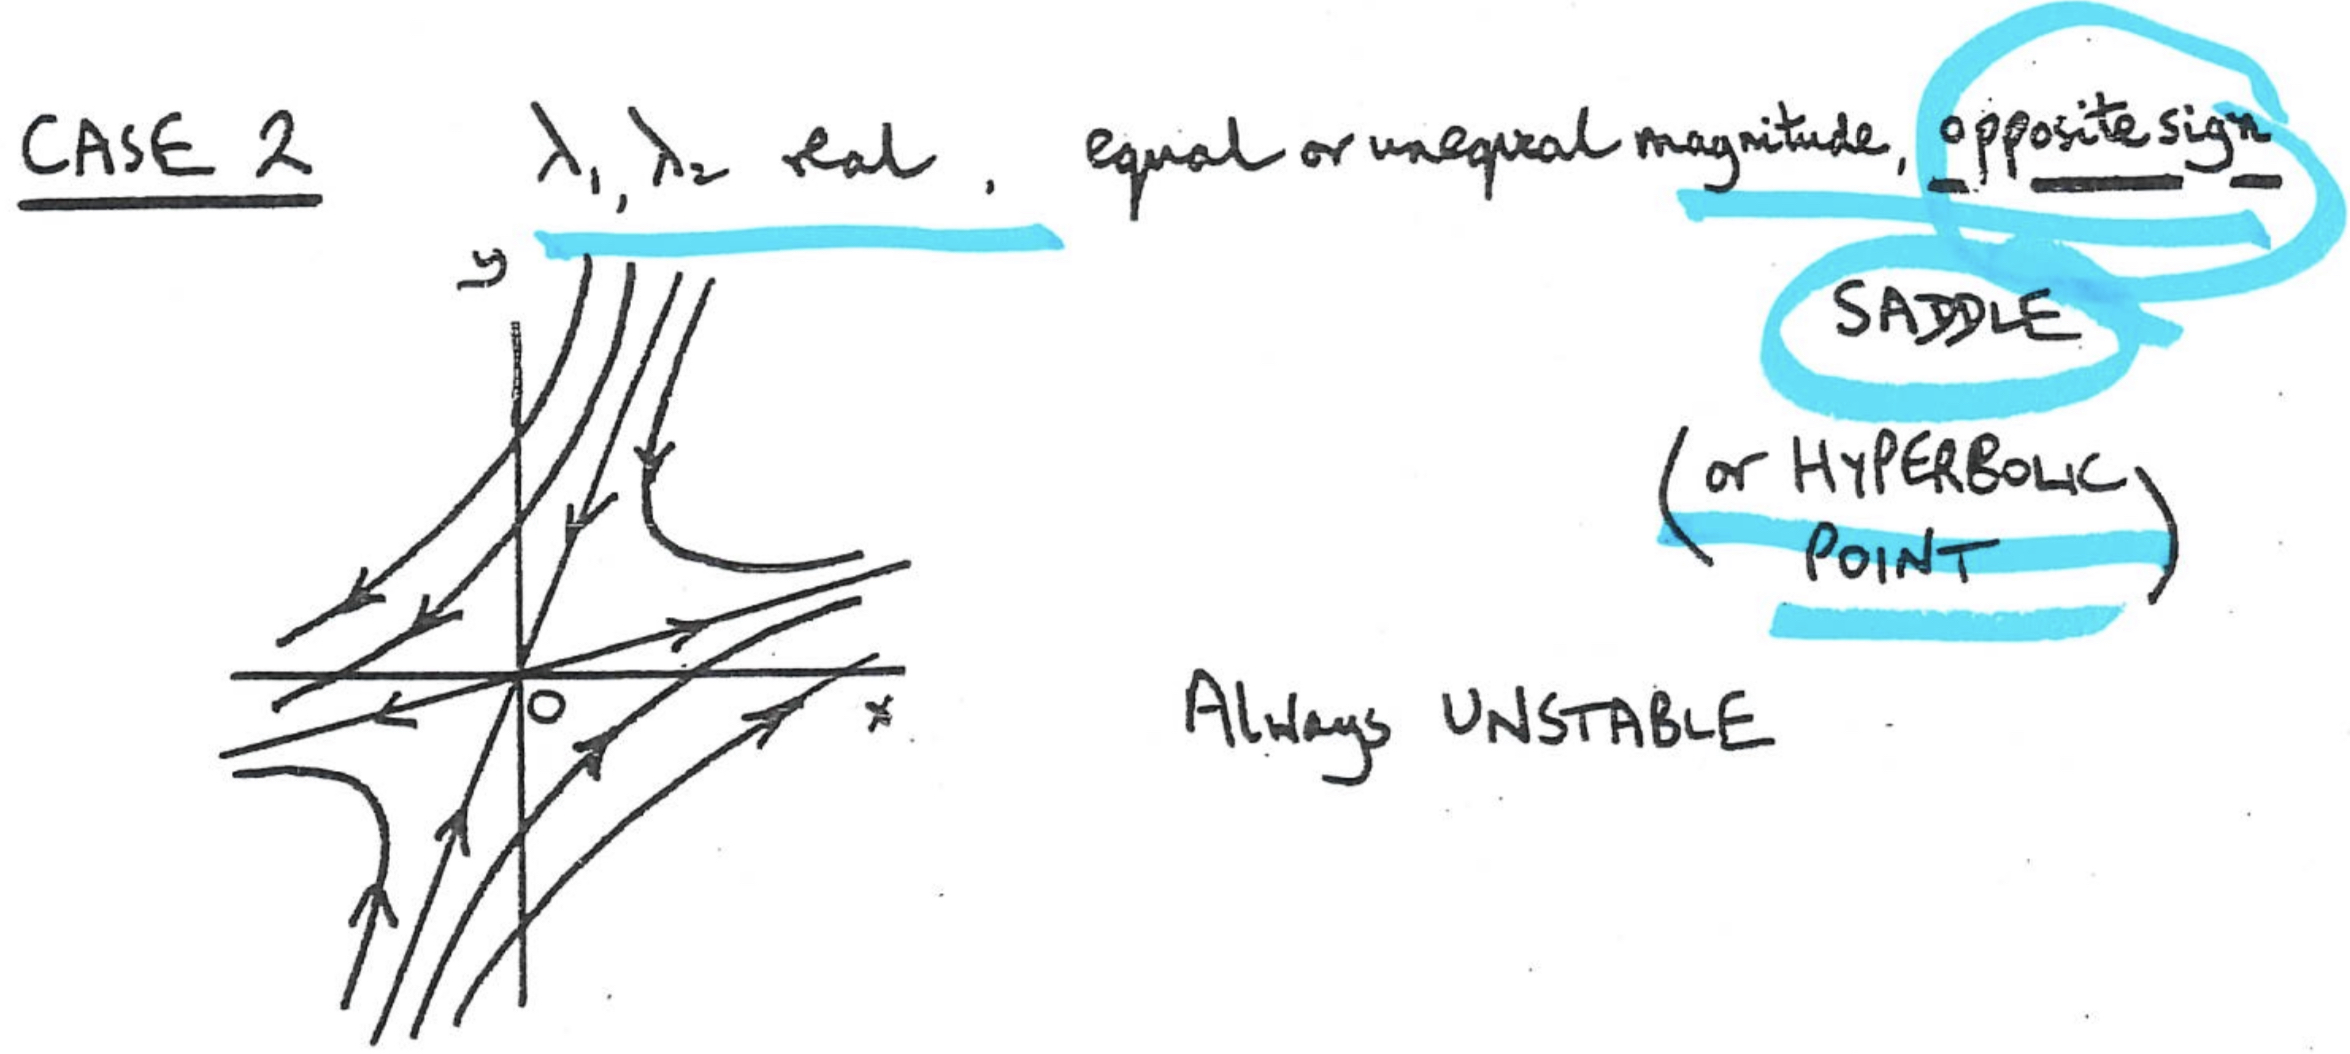
\includegraphics[scale=0.15]{PP2.jpeg}
  	\centering
  	\caption{case 2}\label{PP2}
\end{figure}

\begin{figure}
  	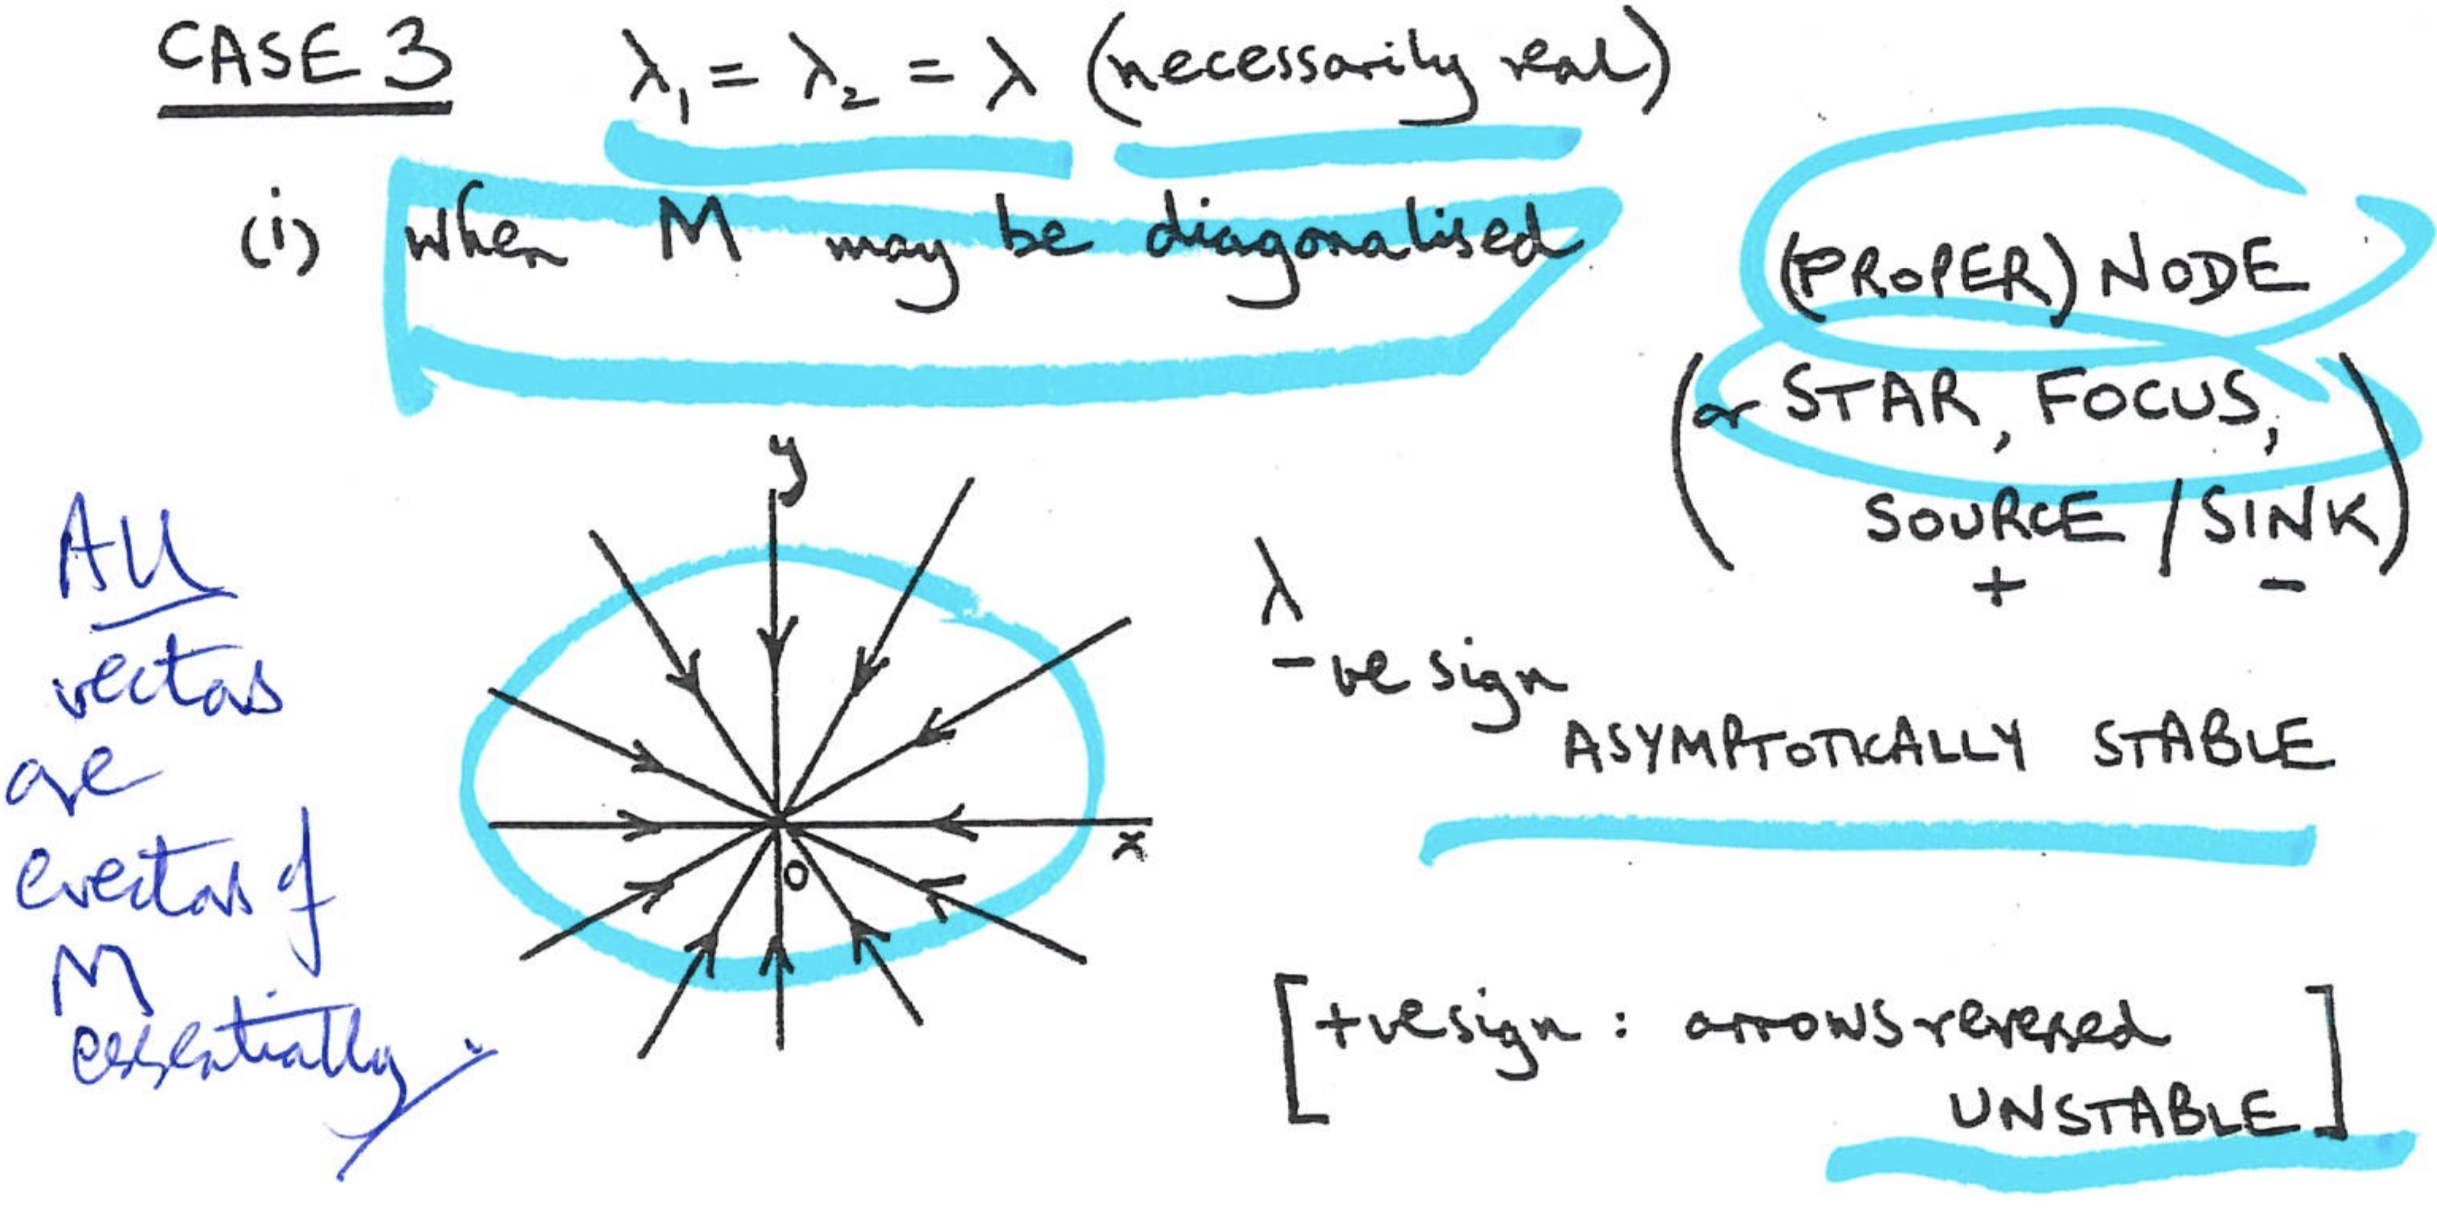
\includegraphics[scale=0.15]{PP3i.jpeg}
  	\centering
    \caption{case 3 (i)}\label{PP3i}
\end{figure}

\begin{figure}
  	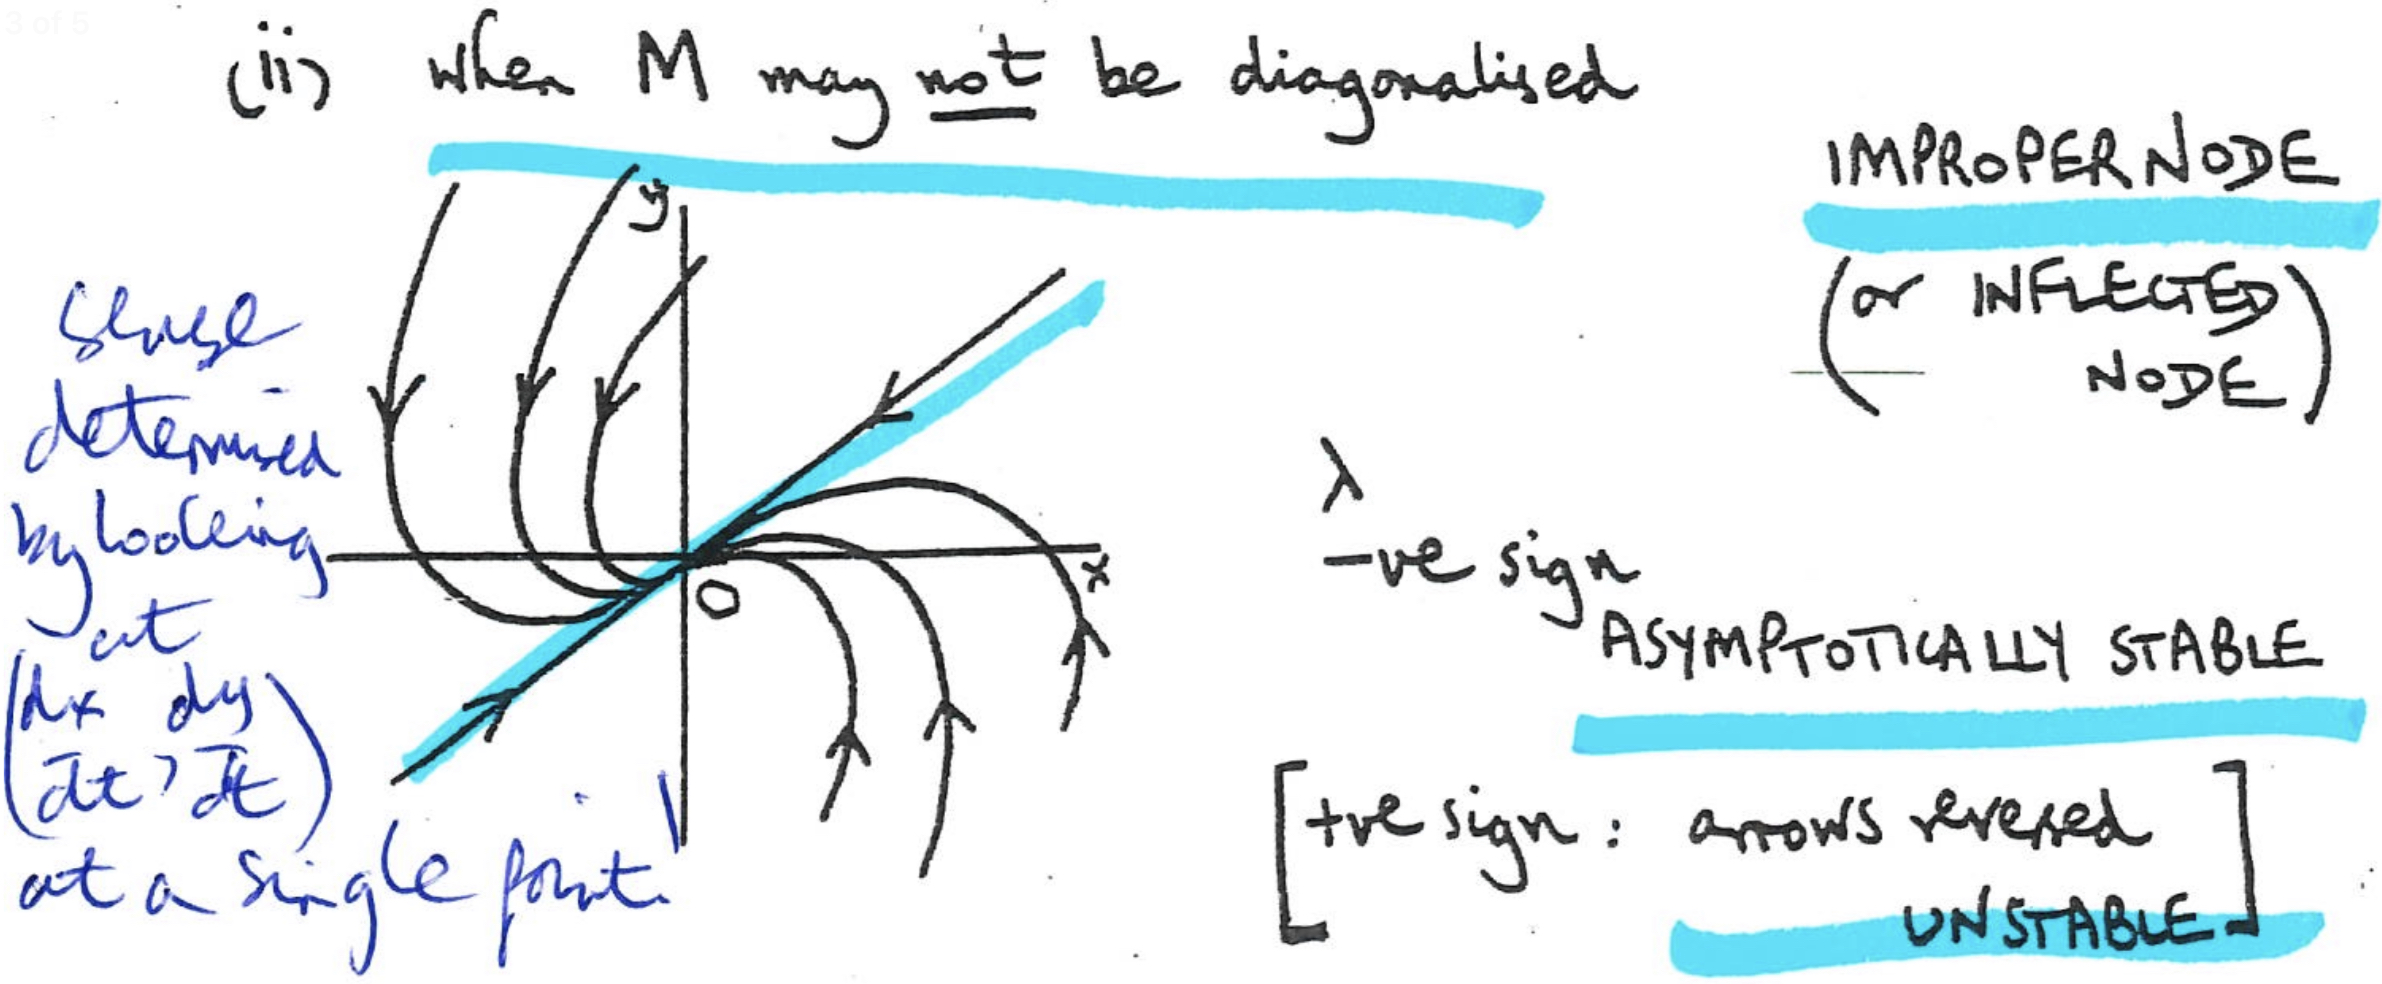
\includegraphics[scale=0.15]{PP3ii.jpeg}
  	\centering
    \caption{case 3 (ii)}\label{PP3ii}
\end{figure}

\begin{figure}
  	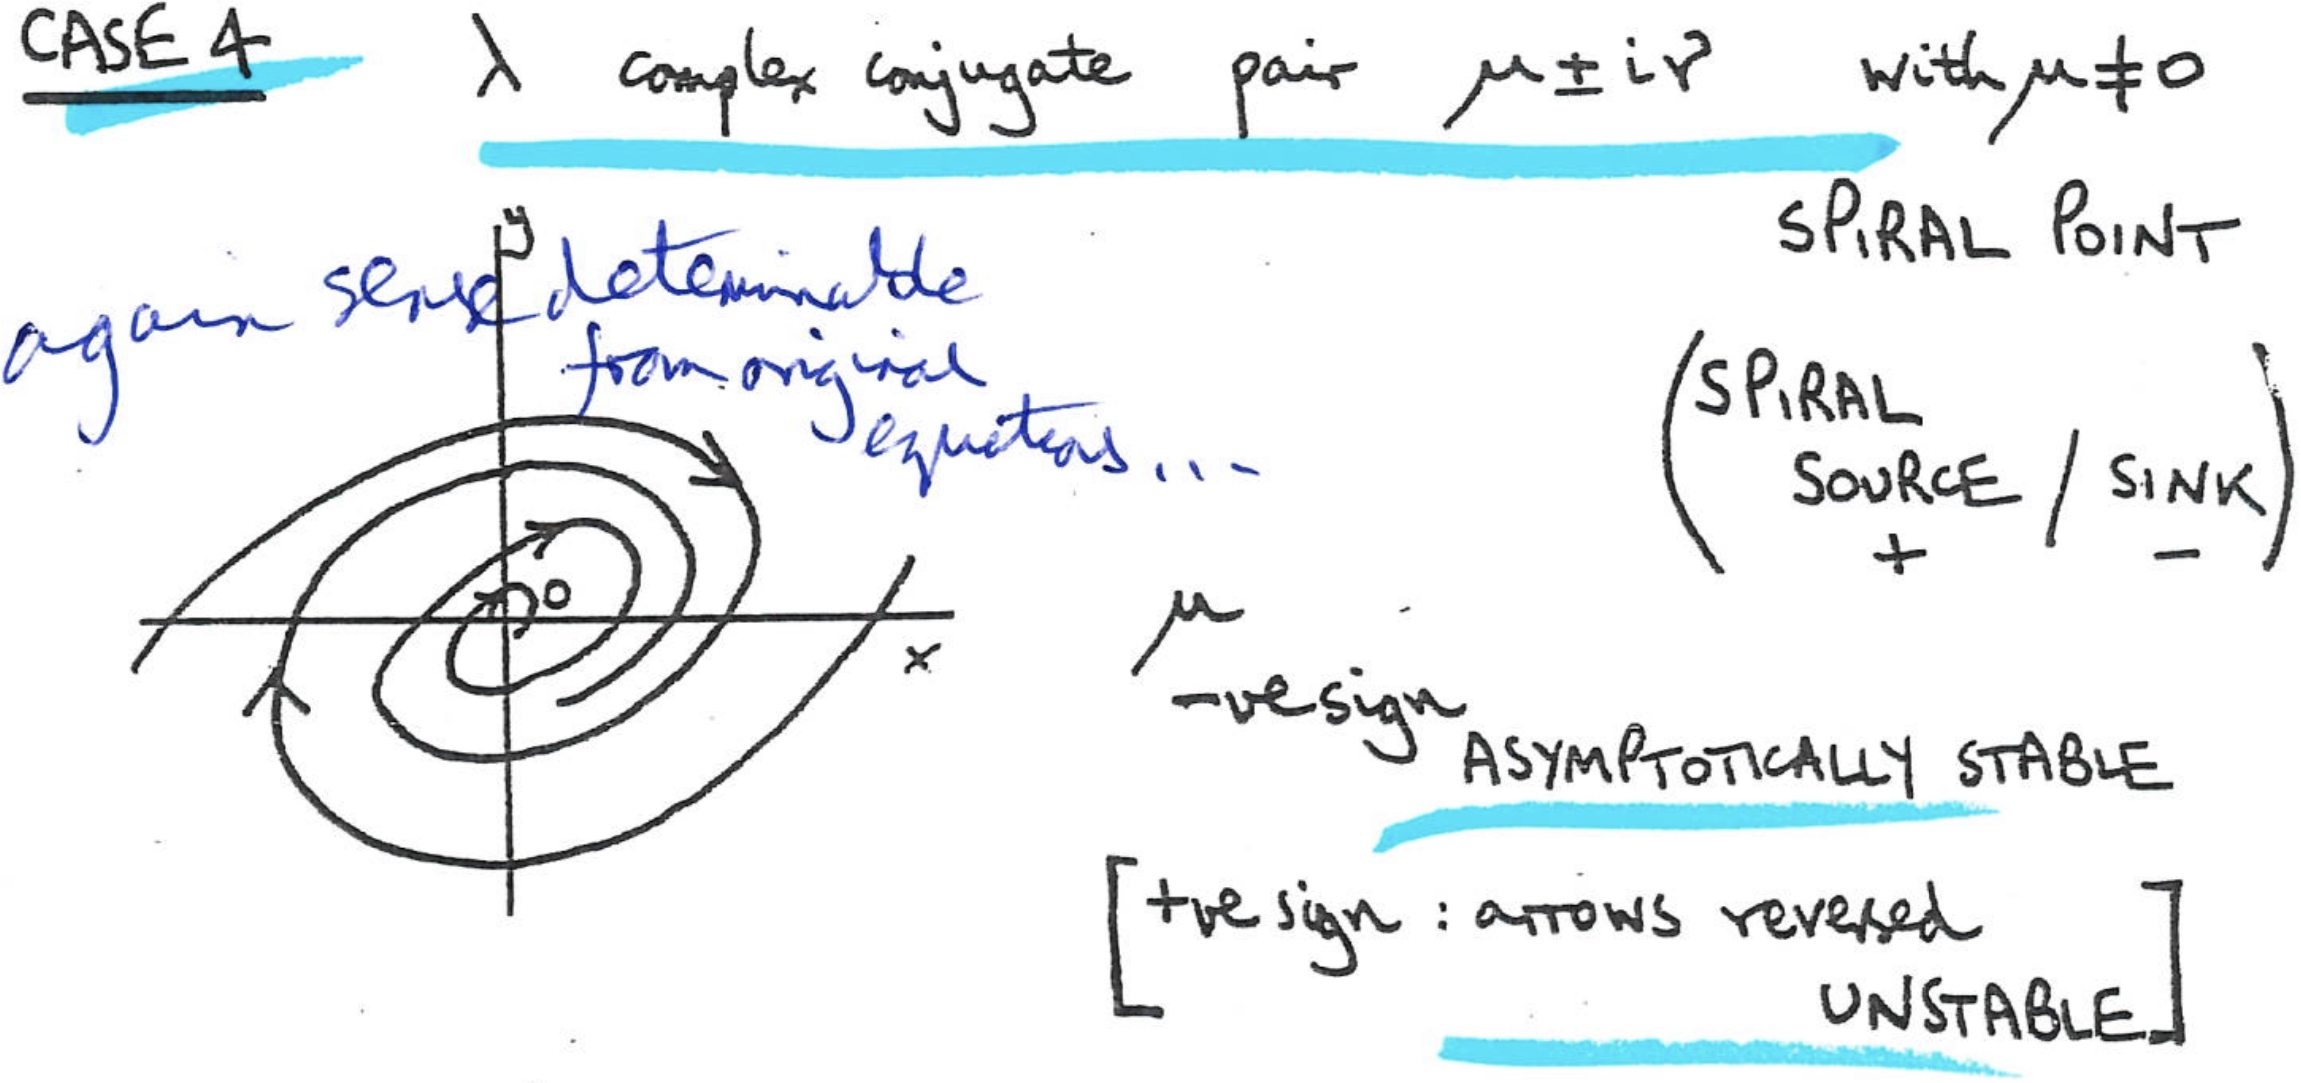
\includegraphics[scale=0.15]{PP4.jpeg}
  	\centering
  	\caption{case 4}\label{PP4}
\end{figure}

\begin{figure}
  	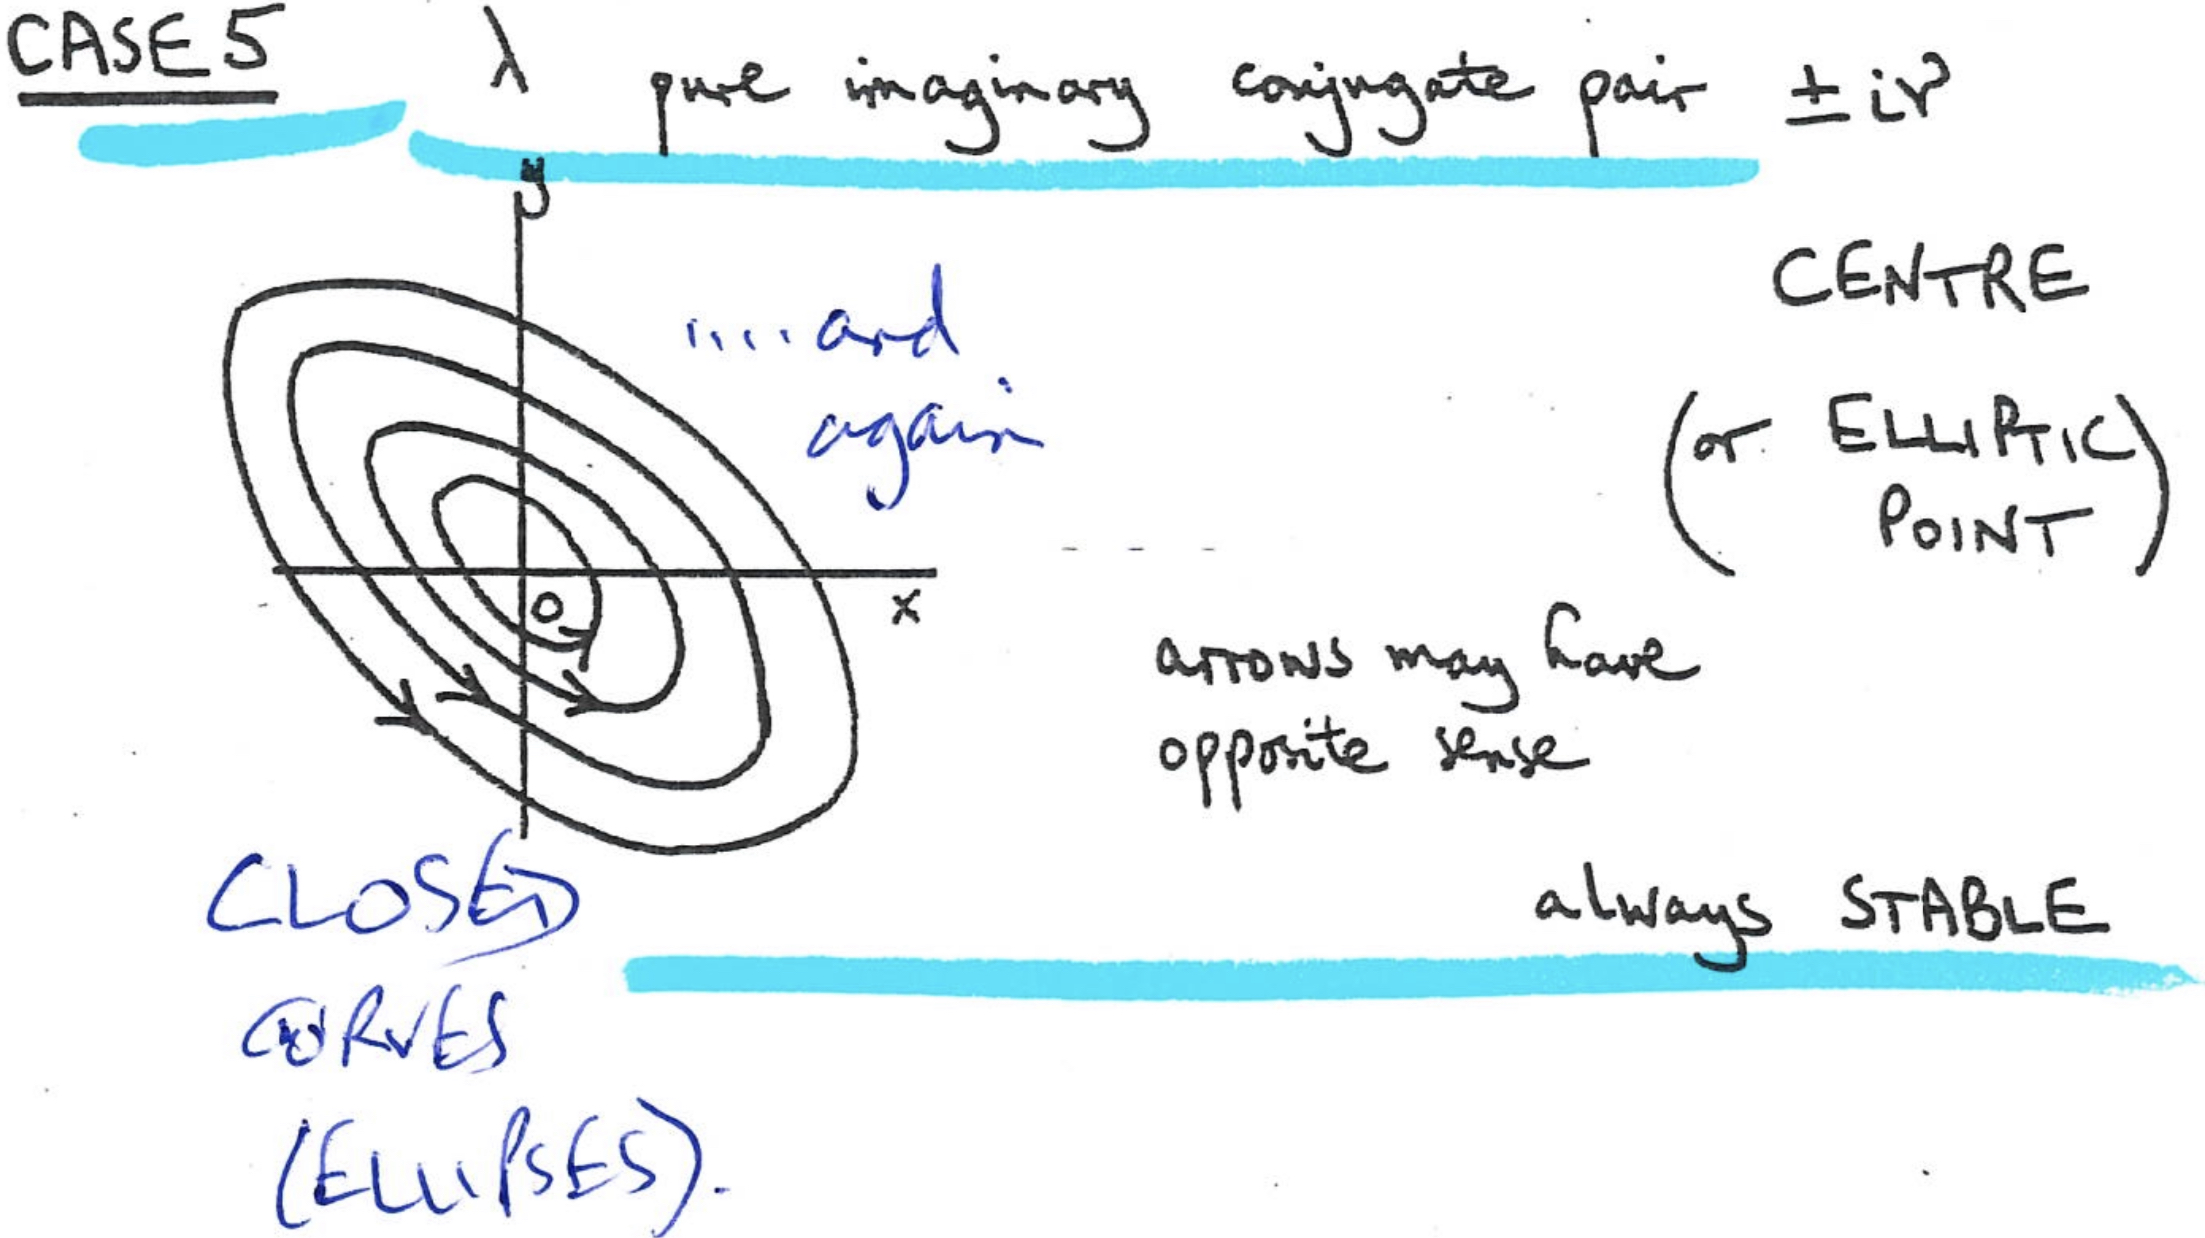
\includegraphics[scale=0.15]{PP5.jpeg}
  	\centering
  	\caption{case 5}\label{PP5}
\end{figure}

Further explanation for case 5: say $x(t)$ and $y(t)$ can be expressed as\[
    \begin{align*}
        x(t) & = A_1 \cos{\nu t} + A_2 \sin{\nu t} \\
        y(t) & = ()A_1 \cos{\nu t} + ()A_2 \sin{\nu t}
    \end{align*}
\]
By solving for $\cos{\nu t}$ and $\sin{\nu t}$, we can see that they are directly proportional to
the different linear combination of $x(t)$ and $y(t)$. By applying the formula
$\cos^{2}{\nu t} + \sin^{2}{\nu t} = 1$,
we derive that the equation for $x$ and $y$ are both at power 2, therefore
we can see that the graph should be \emph{elliptic}.

\begin{ex}
    \,

    \begin{enumerate}[label = (\roman*)]
        \item~\eqref{eqn:5} is `case 2'.

        \item~\eqref{eqn:7} --- the damped harmonic oscillator --- is:
            \begin{itemize}
                    \item $k=0$ corresponds to `case 5'.
                    \item $k^{2} < \omega^{2}$ coresponds to `case 4'.
                    \item $k^{2} > \omega^{2}$ corresponds to `case 1'.
                    \item $k^{2} = \omega^{2}$ corresponds to `case 3(ii)'.
            \end{itemize}
            
        \item $\lambda_1 = \lambda_2$ awkward (case 3(ii)).

            Try solving
            \begin{equation}\label{eqn:8}
                \frac{\mathrm{d}}{\mathrm{d}t} \begin{pmatrix}
                        x \\
                        y
                \end{pmatrix} = \begin{pmatrix}
                1 & -1 \\
                1 & 3
                \end{pmatrix} \begin{pmatrix}
                        x \\
                        y
                \end{pmatrix} 
            \end{equation}
            $\Rightarrow{}\lambda_1 = 2 = \lambda_2$ and we have $\mathbf{V} = \begin{pmatrix}
                    1 \\
                    -1
                \end{pmatrix}$ (\underline{sole} eigenvector here),
                so that $\begin{pmatrix}
                        x \\
                        y
                \end{pmatrix} = B_1 \begin{pmatrix}
                        1 \\
                        -1
                \end{pmatrix} e^{2t}$ is certainly part of our solutions.
                To find the complete solution we can avoid some rather more
                advanced linear algebra by just anticipating a general form 
                for our second part of the solution\[
                    \begin{pmatrix}
                            x \\
                            y
                    \end{pmatrix} = \begin{pmatrix}
                            a \\
                            b
                    \end{pmatrix} t e^{2t} + \begin{pmatrix}
                            c \\
                            d
                    \end{pmatrix} e^{2t}
                \]and find $a, b, c, d$ to  fit!
                Note that $\begin{pmatrix}
                        c \\
                        d
                \end{pmatrix}$ is needed since it does not span the space!
                So $\begin{pmatrix}
                        c \\
                        d
                    \end{pmatrix}$ is not parallel (or antiparallel) to the eigenvector $\begin{pmatrix}
                            1 \\
                            -1
                    \end{pmatrix}$.
                    Substitute into~\eqref{eqn:8}:\[
                        2\begin{pmatrix}
                                a \\
                                b
                        \end{pmatrix} t e^{2t} + \left[\begin{pmatrix}
                                a \\
                                b
                        \end{pmatrix} + 2\begin{pmatrix}
                                c \\
                                d
                        \end{pmatrix} \right] e^{2t}
                        = M\left[\begin{pmatrix}
                                a \\
                                b
                        \end{pmatrix} t e^{2t} + \begin{pmatrix}
                                c \\
                                d
                        \end{pmatrix} e^{2t}\right].
                    \]
                    Equate coefficients respectively of $te^{2t}, e^{2t}$ on each side:\[
                        \left\{\begin{align*}
                            & (M - 2I)\begin{pmatrix}
                                    a \\
                                    b
                            \end{pmatrix} = \begin{pmatrix}
                                    0 \\
                                    0
                            \end{pmatrix} \\
                            & (M - 2I)\begin{pmatrix}
                                    c \\
                                    d
                            \end{pmatrix} = \begin{pmatrix}
                                    a \\
                                    b
                            \end{pmatrix} 
                        \end{align*}\right.
                        \Rightarrow{}\left\{
                            \begin{align*}
                                & \begin{pmatrix}
                                        a \\
                                        b
                                \end{pmatrix} = \mathbf{V} = \begin{pmatrix}
                                        1 \\
                                        -1
                                \end{pmatrix} \;\textnormal{or any multiple} \\
                                & \begin{pmatrix}
                                    -1 & -1 \\
                                    1 & 1
                                \end{pmatrix} \begin{pmatrix}
                                        c \\
                                        d
                                \end{pmatrix} = \begin{pmatrix}
                                        1 \\
                                        -1
                                \end{pmatrix}                             
                            \end{align*}
                        \]\[
                                \Rightarrow{}\begin{pmatrix}
                                        c \\
                                        d
                                \end{pmatrix} = \begin{pmatrix}
                                        K \\
                                        -1-K
                                \end{pmatrix} \;\textnormal{($K$ is arbitrary)}
                    \]
                    Finally we have for this second solution:\[
                        B_2 \begin{pmatrix}
                                1 \\
                                -1
                        \end{pmatrix} t e^{2t} + B_2 \left[\begin{pmatrix}
                                0 \\
                                -1
                        \end{pmatrix} + K\begin{pmatrix}
                                1 \\
                                -1
                        \end{pmatrix} \right] e^{2t}.
                    \]The term with coefficient $K$ is not needed since
                    it has already appeared in the first half of the solution.
                    Thus the general solution is\[
                        \begin{pmatrix}
                                x \\
                                y
                        \end{pmatrix} = B_1\begin{pmatrix}
                                1 \\
                                -1
                        \end{pmatrix} e^{2t} + B_{2} \left[\begin{pmatrix}
                                1 \\
                                -1
                        \end{pmatrix} t e^{2t} + \begin{pmatrix}
                                0 \\
                                -1
                        \end{pmatrix} e^{2t}\right] 
                    \]with two arbitrary constants as required.
            
                \item $\lambda_1 \neq \lambda_2$ but complex pair (case 4/5)

                    \begin{enumerate}[label = (\alph*)]
                        \item \[
                            \frac{\mathrm{d}}{\mathrm{d}t} \begin{pmatrix}
                                    x \\
                                    y
                            \end{pmatrix} = \begin{pmatrix}
                            -\frac{1}{2} & 1 \\
                            -1 & -\frac{1}{2}
                            \end{pmatrix} \begin{pmatrix}
                                    x \\
                                    y
                            \end{pmatrix} 
                        \]$\Rightarrow{}
                        \lambda_1 = -\frac{1}{2} + i, \lambda_2 = -\frac{1}{2}-i$,
                        and we can find eigenvectors formally \[
                            \mathbf{V}_1 = \begin{pmatrix}
                                    1 \\
                                    i
                            \end{pmatrix}, \mathbf{V}_2 = \begin{pmatrix}
                                    1 \\
                                    -i
                            \end{pmatrix}.
                        \]So we have\[
                            \begin{pmatrix}
                                    x \\
                                    y
                            \end{pmatrix} = B_1\begin{pmatrix}
                                    1 \\
                                    i
                            \end{pmatrix} e^{(-\frac{1}{2} + i)t} + B_2 \begin{pmatrix}
                                    1 \\
                                    -i
                            \end{pmatrix} e^{(-\frac{1}{2}-i)t}
                        \]where $B_1, B_2$ are arbitrary. Looking at $\Re$ and $\Im$ parts,\[
                        \begin{align*}
                            \begin{pmatrix}
                                    1 \\
                                    \pm i
                                \end{pmatrix} e^{(-\frac{1}{2}\pm i)t} 
                                & = \begin{pmatrix}
                                        1 \\
                                        \pm i
                                    \end{pmatrix} e^{-\frac{1}{2}t}
                                    (\cos{t} \pm i\sin{t}) \\
                                & = \begin{pmatrix}
                                        e^{-\frac{1}{2}t}\cos{t} \\
                                        -e^{-\frac{1}{2}t}\sin{t}
                                    \end{pmatrix} \pm i\begin{pmatrix}
                                    e^{-\frac{1}{2}t}\sin{t} \\
                                    e^{-\frac{1}{2}t}\cos{t}
                                    \end{pmatrix} 
                        \end{align*}
                        \]\[
                            \Rightarrow{}\begin{pmatrix}
                                    x \\
                                    y
                            \end{pmatrix} = C_1\begin{pmatrix}
                                    e^{-\frac{1}{2}t}\cos{t} \\
                                    -e^{-\frac{1}{2}t}\sin{t}
                            \end{pmatrix} + C_2\begin{pmatrix}
                                    e^{-\frac{1}{2}t}\sin{t} \\
                                    e^{-\frac{1}{2}t}\cos{t}
                            \end{pmatrix} 
                        \]
                        where $C_1 = B_1 + B_2, C_2 = (B_1 - B_2)i$.
                        The form above is best for real initial condition.
                    
                    \item Simple harmonic oscillator ($k = 0$)\[
                        \frac{\mathrm{d}}{\mathrm{d}t} \begin{pmatrix}
                                x \\
                                y
                        \end{pmatrix} = \begin{pmatrix}
                        0 & 1 \\
                        -\omega^{2} & 0
                        \end{pmatrix} \begin{pmatrix}
                                x \\
                                y
                        \end{pmatrix} \iff \frac{\mathrm{d}^{2}x}{\mathrm{d}t^{2}} 
                        + \omega^{2}x = 0, y = \frac{\mathrm{d}x}{\mathrm{d}t}.
                    \]
                    $\Rightarrow{}\lambda_1 = i\omega, \lambda_2 = -i\omega$,
                    $\mathbf{V}_1 = \begin{pmatrix}
                            1 \\
                            i\omega
                        \end{pmatrix} , \mathbf{V}_2 = \begin{pmatrix}
                                1 \\
                                -i\omega
                        \end{pmatrix}$.
                        Therefore,\[
                            \begin{align*}
                            \begin{pmatrix}
                                    x \\
                                    y
                            \end{pmatrix} 
                            & = B_1\begin{pmatrix}
                                    1 \\
                                    i\omega
                            \end{pmatrix} e^{i\omega t} + B_{2} \begin{pmatrix}
                                    1 \\
                                    -i\omega
                            \end{pmatrix} e^{-i\omega t} \\
                            & = C_1 \begin{pmatrix}
                                \cos{\omega t} \\
                                -\omega \sin{\omega t}
                            \end{pmatrix} + C_2\begin{pmatrix}
                            \sin{\omega t} \\
                            \omega \cos{\omega t}
                            \end{pmatrix}.
                            \end{align*}
                        \]
                  \end{enumerate}
    \end{enumerate}
\end{ex}

\subsection{Extensions}

\begin{enumerate}[label = (\roman*)]
    \item inhomogeneous systems\[
        \frac{\mathrm{d}}{\mathrm{d}t} \begin{pmatrix}
                x \\
                y
        \end{pmatrix} - M\begin{pmatrix}
                x \\
                y
        \end{pmatrix} = \begin{pmatrix}
        f_1(t) \\
        f_2(t)
        \end{pmatrix}
    \]can be solved by the standard method we used for simple linear ordinary differential equations\[
        \begin{pmatrix}
                x \\
                y
            \end{pmatrix}_{\textnormal{GS}} = \begin{pmatrix}
                    x \\
                    y
                \end{pmatrix}_{\textnormal{CF}} + \begin{pmatrix}
                        x \\
                        y
                    \end{pmatrix}_{\textnormal{PI}}
    \]
    We solved CF earlier in this chapter. For PI, it is very difficult in general.
    Here1 we just need to find any single particular solution for simple cases such as
    $f_1$ and $f_2$ are constants, so the let PI be a constant vector, and solve for it will do.

\item higher order systems

    The whole process may be generalised, e.g.\[
        \frac{\mathrm{d}}{\mathrm{d}t} \begin{pmatrix}
                x \\
                y \\
                z
        \end{pmatrix} = \begin{pmatrix}
        1 & 1 & 2 \\
        1 & 2 & 1 \\
        2 & 1 & 1
        \end{pmatrix} \begin{pmatrix}
                x \\
                y \\
                z
        \end{pmatrix}.
    \]
    Since $\det{(M - \lambda I)} = 0$, $\lambda^{3} - 4 \lambda^{2} - \lambda + 4 = 0$,\[
        \lambda_1 = 4, \lambda_2 = 1, \lambda_3 = -1,
        \mathbf{V}_1 = \begin{pmatrix}
                1 \\
                1 \\
                1
        \end{pmatrix} , \mathbf{V}_2 = \begin{pmatrix}
                1 \\
                -2 \\
                1
        \end{pmatrix} , \mathbf{V}_3 = \begin{pmatrix}
                1 \\
                0 \\
                -1
        \end{pmatrix}
    \]\[
        \Rightarrow{}\begin{pmatrix}
                x \\
                y \\
                z
        \end{pmatrix} = B_1\begin{pmatrix}
                1 \\
                1 \\
                1
        \end{pmatrix} e^{4t} + B_2\begin{pmatrix}
                1 \\
                -2 \\
                1
        \end{pmatrix} e^{t} + B_3\begin{pmatrix}
                1 \\
                0 \\
                -1
        \end{pmatrix} e^{-t}.
    \]
    It is also possible to have equal roots, or complex conjugate pair!
\end{enumerate}

\section{Partial Differentiation}

\subsection{Introduction}

Consider a function $u = u(x,y)$ of 2 independent variables $x, y$.
We can think of $u$ as being the height of a surface above the $(x,y)$ plane.
It is often helpful to visualize the surface using \emph{contour lines}\[
    u(x,y) = C
\]for different values of $c$, which is a constant.
The countour lines are marked with the value $C$ which $u(x,y)$ would give.

Physically $u$ could represent a geometrical object or temperature or pressure or \ldots
We now look at (spatial) rates of change.
Firstly, start at $P(x,y)$ and move a small distance $\delta x = h$ in the $x$ direction
to $Q(x+h,y)$ i.e.\ keeping $y$ fixed. 

\newmdtheoremenv[style=defEnv]{partial differentiation}[theorem]{Definition}
\begin{partial differentiation}
We define (if the limit exists):\[
    \frac{\partial u}{\partial x} = \lim_{h\rightarrow{}0}
    \left[\frac{u(x+h, y) - u(x,y)}{h}\right] 
\]as the rate of change of $u$ with respect to $x$ at $P$ (keeping $y$ fixed).
\end{partial differentiation}
\textbf{\underline{Notations}}: $\frac{\partial u}{\partial x} , 
{\left(\frac{\partial u}{\partial x} \right)}_y,
u_x,\ldots$
Be careful with the subscripts!

\medskip
Similarly, for $P(x,y) \rightarrow{}P(x, y+k)$, we define:\[
    \frac{\partial u}{\partial y} = \lim_{k\rightarrow{}0}\left[
    \frac{u(x,y+k) - u(x,y)}{k}\right] 
\]as the rate of change of $u$ with respect to $y$ at $P$ (keeping $x$ fixed).
The notations: $\frac{\partial u}{\partial y} , 
{\left(\frac{\partial u}{\partial y} \right)}_x,
u_y,\ldots$

\paragraph{Examples}
\,

\begin{enumerate}[label = (\roman*)]
    \item $u = x^{2}\sin{y} + y^{3}$\[
        \Rightarrow{}\frac{\partial u}{\partial x} = 2x\sin{y},\quad
        \frac{\partial u}{\partial y} x^{2}\cos{y} + 3y^{2}.
    \]
    We can, of course, consider higher derivatives:\[
        \frac{\partial^{2}u}{\partial x^{2}} 
        = \frac{\partial }{\partial x} \left(\frac{\partial u}{\partial x} \right) 
        = u_{xx}, \quad
        \frac{\partial^{2}u}{\partial x \partial y} 
        = \frac{\partial}{\partial x} \left(\frac{\partial u}{\partial y} \right) 
        = u_{xy}
    \]
    Note the order of the partial differentiation in the second expression.
    For the example above we have\[
        \begin{align*}
            \frac{\partial^{2}u}{\partial x^{2}} & = 2\sin{y}, & \frac{\partial^{2}u}{\partial y^{2}} & = -x^{2}\sin{y} + 6y, \\ 
            \frac{\partial^{2}u}{\partial y \partial x} & = 2x\cos{y}, & \frac{\partial^{2}u}{\partial x \partial y} & = 2x\cos{y}.
        \end{align*}
    \]
    We note that, in this case, $\frac{\partial^{2}u}{\partial x \partial y}
    = \frac{\partial^{2}u}{\partial y \partial x} $, which is a general result,
    requiring only continuity of LHS and RHS --- usually the case.
    E.g. $\frac{x-y}{x+y}$ is not continuous at $(x,y) = (0,0)$.

    Similarly, we generally have $u_{xxyyx} = u_{yxyxx} = \ldots$.

\item $u(x,y) = a\sin{(x - ct)}$\[
    \begin{align*}
        \frac{\partial u}{\partial x} & = a\cos{(x-ct)}, & \frac{\partial^{2}u}{\partial x^{2}} & = -a\sin{(x-ct)}, \\
        \frac{\partial u}{\partial t} & = -ac\cos{(x-ct)}, & \frac{\partial^{2}u}{\partial t^{2}} & = -ac^{2}\sin{(x-ct)}.
    \end{align*}
\]
We can see that $u(x,t)$ satisfies\[
    \frac{\partial^{2}u}{\partial x^{2}} = \frac{1}{c^{2}} \frac{\partial^{2}u}{\partial t^{2}} 
\]which is a 2nd order linear P.D.E.
It is the one-dimensional wave equation.

In fact, any reasonable function $f(x-ct)$ will satisfy this equation!
It represents a wave form moving (with $c>0$ here) to the right.
(if $c<0$, then moving to the left)

\item $u = \tan^{-1}{\frac{y}{x}}$.
    This satisfies\[
        \nabla^{2} u = \frac{\partial^{2}u}{\partial x^{2}} + \frac{\partial^{2}u}{\partial y^{2}} = 0.
    \]which is a second order linear P.D.E.
    It is famously known as the Laplace's equation.
\end{enumerate}

\subsection{The Total Differential}

When we have a function of a single varialbe $f(x)$,
and we make a small change $x \rightarrow{} x + \delta x$
so that $f \rightarrow{} f + \delta f$, then 
$\delta f \approx \frac{\mathrm{d}f}{\mathrm{d}x} \delta x$.
In the limit (``small, $\rightarrow{}0$'')\[
    \mathrm{d}f = \frac{\mathrm{d}f}{\mathrm{d}x} \mathrm{d}x.
\]
Now for a function of two variables, small changes $x \rightarrow{} x + \delta x$,
$y \rightarrow{} y + \delta y$ lead to $u(x,y) \rightarrow{} u + \delta u$,
with $\delta u = u(x+\delta x, y+\delta y) - u(x,y)$, so
$\delta u \approx \frac{\partial u}{\partial x} \delta x + \frac{\partial u}{\partial y} \delta y$.

\newmdtheoremenv[style=defEnv]{total differential}[theorem]{Definition}
\begin{total differential}
    The \textbf{\emph{total differential}} of $u(x,y)$ is\[
    \mathrm{d}u = \frac{\partial u}{\partial x} \mathrm{d}x + \frac{\partial u}{\partial y} \mathrm{d}y.
\]
The idea can be generalized to higher dimensions, e.g. $u(x,y,z)$ etc.
\end{total differential}

\paragraph{Examples}
\,

\begin{enumerate}[label = (\roman*)]
    \item $u = x^{2}\sin{y} + y^{3}$, and we can get\[
            \delta u \approx (2x\sin{y})\delta x + (x^{2}\cos{y} + 3y^{2})\delta y
    \]\[
    \mathrm{d}u = (2x\sin{y})\mathrm{d}x + (x^{2}\cos{y} + 3y^{2})\mathrm{d}y.
    \]

\item Area of a rectangle $A = xy$. Here\[
    \begin{align*}
        \delta A & = (x + \delta x)(y + \delta y) - xy \\
                 & = \underbrace{y\delta x + x\delta y}_\text{1st order small} 
                 + \underbrace{\delta x \delta y}_\text{2nd order small}
    \end{align*}
\]Therefore $\delta A \approx y \delta x + x \delta y \iff
\mathrm{A} = y \mathrm{d}x + x\mathrm{d}y$.

\item Height of a building $h = x\tan{\theta}$.

    Let $x = 200$m with error $\pm 2$m, $\theta$ = 20\textdegree\ with error $\pm \frac{1}{2}$\textdegree.
    We can derive that\[
        \delta h \approx (\tan{\theta})\delta x + (x\sec^{2}{\theta})\delta\theta.
    \]
    Central estimate is $200\tan{\left(\frac{\pi}{9}\right)} = 72.8$m.\[
        \Rightarrow{}\delta h \approx 0.36\delta x + 226.5\delta\theta
    \]with $|\delta x| \le 2, |\delta \theta|\le \frac{\pi}{360} = 0.0087$. So\[
    |\delta h| \le (0.36)(2) + (226.5)(0.0087) = 2.7\textnormal{m}
\]and $h = 72.8 \pm 2.7$m. (which is $\pm 3.7\%$)
\end{enumerate}

\subsection{Function of a function --- `The Chain Rule'}

If we have $u = f(x)$ and $x = g(t)$, then we have as a consequence\[
    \frac{\mathrm{d}u}{\mathrm{d}t} = \frac{\mathrm{d}u}{\mathrm{d}x} \cdot \frac{\mathrm{d}x}{\mathrm{d}t} 
    = f'(x)g'(t) = f'(g(t))g'(t).
\]
Now consider $u = u(x,y)$ where $x(t)$ and $y(t)$. We saw previously that\[
\delta u \approx \frac{\partial u}{\partial x} \delta x + \frac{\partial u}{\partial y} \delta y
\quad\Longrightarrow{}\quad \frac{\delta u}{\delta t} \approx \frac{\partial u}{\partial x}
\frac{\delta x}{\delta t} + \frac{\partial u}{\partial y} \frac{\delta y}{\delta t}.
\]

\newmdtheoremenv[style=defEnv]{the chain rule}[theorem]{Definition}
\begin{the chain rule}
    The chain rule in 3-dimension is\[
        \frac{\mathrm{d}u}{\mathrm{d}t} = \frac{\partial u}{\partial x} 
        \frac{\mathrm{d}x}{\mathrm{d}t} + \frac{\partial u}{\partial y} \frac{\mathrm{d}y}{\mathrm{d}t} 
    \]where $x$ and $y$ are functions \emph{only} of $t$.
\end{the chain rule}

E.g.\ if $x(r,s)$ and $y(r,s)$ then\[
    \frac{\partial \overline{u}}{\partial r} = \frac{\partial \overline{u}}{\partial x} 
    \frac{\partial x}{\partial r} + \frac{\partial \overline{u}}{\partial y} \frac{\partial y}{\partial r},\quad
    \frac{\partial \overline{u}}{\partial s} = \frac{\partial \overline{u}}{\partial x}
    \frac{\partial x}{\partial s} + \frac{\partial \overline{u}}{\partial y} \frac{\partial y}{\partial s}.
\]

\paragraph{Examples}
\,

\begin{enumerate}[label = (\roman*)]
    \item Volume $V$ of a cylindrical box of radius $r$ and height $h$: $V = \pi r^{2}h$.

        If we know that $r = 2t, h = 1 + t^{2}$, then\[
            \begin{align*}
                \frac{\mathrm{d}V}{\mathrm{d}t} & = \frac{\partial V}{\partial r} \frac{\mathrm{d}r}{\mathrm{d}t} 
                + \frac{\partial V}{\partial h} \frac{\mathrm{d}h}{\mathrm{d}t} \\
                                                & = (2\pi rh)(2) + (\pi r^{2})(2t) \\
                                                & = 8\pi (t + 2t^{3})
            \end{align*}
        \]
        \underline{Check}: $V = \pi{(2t)}^{2}(1+t^{2}) = 4\pi(t^{2}+t^{4})$,
        and of course $\frac{\mathrm{d}V}{\mathrm{d}t} = 8\pi t + 16\pi t^{3}$.

    \item $u(x,y) = \overline{u}(s,t) = x^{2}y$ with $x = st$, $y = s + t$.
        \[
            \Rightarrow{}\left\{\begin{align*}
                    \frac{\partial \overline{u}}{\partial s} & = \frac{\partial u}{\partial x} 
                    \frac{\partial x}{\partial s} + \frac{\partial u}{\partial y} \frac{\partial y}{\partial s} 
                    = (2xy)(t) + (x^{2})(1) = \cdots = 3s^{2}t^{2} + 2st^{3} \\
                    \frac{\partial \overline{u}}{\partial t} & = \frac{\partial u}{\partial x}
                    \frac{\partial x}{\partial t} + \frac{\partial u}{\partial y} \frac{\partial y}{\partial t}
                    = (2xy)(s) + (x^{2})(1) = \cdots = 3s^{2}t^{2} + 2s^{3}t.
            \end{align*}\right.
        \]
        Again, we can check this since $u(x,y) = {(st)}^{2}(s+t) = \overline{u}(s,t)$.

    \item $u(x,y) = xy + y^{2}$, a \emph{cautionary} example!

        If we have a second relation $y = x + t$, then of course\[
            \overline{u}(x,t) = x(x+t) + {(x + t)}^{2}.
        \]
        We have to be careful when we look at the variation of $u$ and $\overline{u}$ with respect to $x$:
        \begin{enumerate}[label = (\alph*)]
            \item $\frac{\partial u}{\partial x} = y (= x + t)$
            \item $\frac{\partial \overline{u}}{\partial x} = 2x + t + 2(x + t) (= 4x + 3t)$.
        \end{enumerate}
        These are not the same --- $u$ and $\overline{u}$ have the same function values
        at corresponding points. But in (a), $y$ is being kept constant ${\left(\frac{\partial u}{\partial x} \right)}_{y}$,
        and in (b), $t$ is being kept constant ${\left(\frac{\partial \overline{u}}{\partial x} \right)}_{t}$,
        So care is needed evidently! Ensure that the substitution is \emph{disjoint}!
\end{enumerate}

\subsection{From Cartesians to Polars}
\[
    \underbrace{u(x,y)}_\text{Cartesians} = \underbrace{\overline{u}(r,\theta)}_\text{Plane Polars}
\]with\[
    \left\{\begin{align*}
            x & = r\cos{\theta} \\
            y & = r\sin{\theta}
    \end{align*}\right.,\qquad \left\{\begin{align*}
            r & = {(x^{2} + y^{2})}^{\frac{1}{2}} \\
            \theta & = \tan^{-1}{\frac{y}{x}}
    \end{align*}\right..
\]
Both are \emph{orthogonal} systems!
We need to be careful! E.g.\[
    {\left(\frac{\partial x}{\partial r} \right)}_{\theta} = \cos{\theta} \quad\textnormal{and}\quad
    {\left(\frac{\partial r}{\partial x} \right)}_{y} = \frac{x}{{(x^{2} + y^{2})}^{\frac{1}{2}}} = \cos{\theta}.
\]
They are keeping different constants, so we should \emph{not} be tempted! \[
    {\left(\frac{\partial x}{\partial r} \right)}_{\theta} \neq
    \frac{1}{{\left(\frac{\partial r}{\partial x} \right)}_{y}}.
\]
\underline{Note}: The Cartesian and Polar versions of our function
have the same function values, but are described differently! E.g.\[
    u(x,y) = x^{2}+y^{2} = r^{2} = \overline{u}(r,\theta)
\]and it is not $(r^{2} + \theta^{2})$.

\subsubsection{Chain rule}

\[
    \begin{align*}
        \frac{\partial u}{\partial x} & = \frac{\partial \overline{u}}{\partial r} \frac{\partial r}{\partial x}
        + \frac{\partial \overline{u}}{\partial \theta} \frac{\partial\theta}{\partial x} \\
                                      & = (\cos{\theta})\frac{\partial \overline{u}}{\partial r}
                                      + \left(-\frac{\sin{\theta}}{r}\right) \frac{\partial \overline{u}}{\partial \theta}
    \end{align*}
\]and\[
    \begin{align*}
        \frac{\partial u}{\partial y} & = \frac{\partial \overline{u}}{\partial r} \frac{\partial r}{\partial y}
        + \frac{\partial \overline{u}}{\partial \theta} \frac{\partial\theta}{\partial y} \\
                                      & = (\sin{\theta})\frac{\partial \overline{u}}{\partial r} 
                                      + \left(\frac{\cos{\theta}}{r}\right) \frac{\partial \overline{u}}{\partial \theta}.
    \end{align*}
\]

\newmdtheoremenv[style=defEnv]{partial differential operators}[theorem]{Definition}
\begin{partial differential operators}
    The \textbf{\emph{partial differential operators}} are defined as\[
        \begin{align*}
            \frac{\partial}{\partial x} & = \cos{\theta}\frac{\partial}{\partial r}
            - \frac{\sin{\theta}}{r}\frac{\partial}{\partial \theta} \\
            \frac{\partial}{\partial y} & = \sin{\theta}\frac{\partial}{\partial r} 
            + \frac{\cos{\theta}}{r}\frac{\partial}{\partial \theta}
        \end{align*}
    \]which relate rates of change in the two different coordinate systems!
\end{partial differential operators}

\paragraph{Examples}
\,

\begin{enumerate}[label = (\roman*)]
    \item $u(x,y) = x^{2}-y^{2} = r^{2}(\cos^{2}{\theta} - \sin^{2}{\theta}) = \overline{u}(r,\theta)$.\[
        \frac{\partial u}{\partial x} = 2x = 2r\cos{\theta}, \quad
        \frac{\partial u}{\partial y} = -2y = -2r\sin{\theta}.
    \]

\item We can express 
    % Why do the brackets appear to be of different size?
    ${\left(\frac{\partial u}{\partial x}\right)}^{2} + {\left(\frac{\partial u}{\partial y}\right)}^{2}$
    in plane polars as\[
        \begin{align*}
        {\left[(\cos{\theta})\frac{\partial \overline{u}}{\partial r} 
        + \left(-\frac{\sin{\theta}}{r}\right) \frac{\partial \overline{u}}{\partial \theta} \right]}^{2}
        & + {\left[(\sin{\theta})\frac{\partial \overline{u}}{\partial r} 
        + \left(\frac{\cos{\theta}}{r}\right) \frac{\partial \overline{u}}{\partial \theta} \right]}^{2} \\
        & = {\left(\frac{\partial \overline{u}}{\partial r} \right)}^{2}
        + \frac{1}{r^{2}} {\left(\frac{\partial \overline{u}}{\partial \theta} \right)}^{2}.
        \end{align*}
    \]

\item For Laplace equation $\frac{\partial^{2}u}{\partial x^{2}} + \frac{\partial^{2}u}{\partial y} = 0$,\[
    \begin{align*}
        \frac{\partial^{2}u}{\partial x^{2}}
        & = \frac{\partial}{\partial x} \left(\frac{\partial u}{\partial x} \right)
        = \left(\cos{\theta} \frac{\partial}{\partial r} 
        - \frac{\sin{\theta}}{r} \frac{\partial}{\partial \theta} \right)
        \left(\cos{\theta} \frac{\partial \overline{u}}{\partial r} 
        - \frac{\sin{\theta}}{r}\frac{\partial \overline{u}}{\partial \theta} \right) \\
        & \;\vdots \quad\textnormal{Attrition!} \\
        & \begin{aligned}[t]
        = \cos^{2}{\theta}\frac{\partial^{2} \overline{u}}{\partial r^{2}} 
        - \frac{2\cos{\theta}\sin{\theta}}{r} \frac{\partial^{2} \overline{u}}{\partial r \partial \theta} 
        & + \frac{\sin^{2}{\theta}}{r} \frac{\partial \overline{u}}{\partial r} \\
        & + \frac{\sin^{2}{\theta}}{r^{2}}\frac{\partial^{2}\overline{u}}{\partial \theta^{2}} 
        + \frac{2\sin{\theta}\cos{\theta}}{r^{2}}\frac{\partial \overline{u}}{\partial \theta}
        \end{aligned}
    \end{align*}
\]and\[
    \begin{align*}
        \frac{\partial^{2}u}{\partial y^{2}}
        & = \frac{\partial}{\partial y} \left(\frac{\partial u}{\partial y} \right)
        = \left(\sin{\theta} \frac{\partial}{\partial r} 
        + \frac{\cos{\theta}}{r} \frac{\partial}{\partial \theta} \right)
        \left(\sin{\theta} \frac{\partial \overline{u}}{\partial r} 
        + \frac{\cos{\theta}}{r}\frac{\partial \overline{u}}{\partial \theta} \right) \\
        & \;\vdots \quad\textnormal{Attrition!} \\
        & \begin{aligned}[t]
        = \sin^{2}{\theta}\frac{\partial^{2} \overline{u}}{\partial r^{2}} 
        + \frac{2\cos{\theta}\sin{\theta}}{r} \frac{\partial^{2} \overline{u}}{\partial r \partial \theta} 
        & + \frac{\cos^{2}{\theta}}{r} \frac{\partial \overline{u}}{\partial r} \\
        & + \frac{\cos^{2}{\theta}}{r^{2}}\frac{\partial^{2}\overline{u}}{\partial \theta^{2}} 
        - \frac{2\sin{\theta}\cos{\theta}}{r^{2}}\frac{\partial \overline{u}}{\partial \theta}.
        \end{aligned}
    \end{align*}
\]
Hence\[
    \frac{\partial^{2}u}{\partial x^{2}} + \frac{\partial^{2}u}{\partial y^{2}}
    = \underbrace{\frac{\partial^{2}\overline{u}}{\partial r^{2}} + \frac{1}{r}
    \frac{\partial \overline{u}}{\partial r}}_\text{$=\frac{1}{r}\frac{\partial}{\partial r} 
\left(r\frac{\partial \overline{u}}{\partial r} \right) $} 
    + \frac{1}{r^{2}} \frac{\partial^{2}\overline{u}}{\partial \theta^{2}} = 0.
\]
Laplace in 3 dimensions is\[
    \frac{\partial^{2}u}{\partial x^{2}} + \frac{\partial^{2}u}{\partial y} + \frac{\partial^{2}u}{\partial z} = 0.
\]
\end{enumerate}

\subsection{Implicit Functions}

If we have a function defined implicitly $F(x,y) = 0$,
then $F$ does not change as $x$ and $y$ do so.
The total derivative then is\[
    \mathrm{d}F = \frac{\partial F}{\partial x} \mathrm{d}x + \frac{\partial F}{\partial y} \mathrm{d}y = 0.
\]So the derivative of $y$ with respect to $x$ is given by\[
    \frac{\mathrm{d}y}{\mathrm{d}x} = -\frac{F_x}{F_y}.
\]

\paragraph{Examples}
\,

\begin{enumerate}[label = (\roman*)]
    \item $F(x,y) = x^{2}\sin{y} + xy - 1 = 0$, then\[
            \frac{\mathrm{d}y}{\mathrm{d}x} = -\frac{2x\sin{y}+y}{x^{2}\cos{y}+x}.
    \]
    If we have an implicit function of 3 variables $F(x,y,z) = 0$, 
    this constrains our point $(x,y,z)$ to be on a particular surface.
    We can certainly regard, if we wish, $x= x(y,z)$ or $y = y(x,z)$ or $z = z(x,y)$.
    Now, no change in $F$ on the surface,\[
        \Rightarrow{}\mathrm{d}F = \frac{\partial F}{\partial x} \mathrm{d}x
        + \frac{\partial F}{\partial y} \mathrm{d}y + \frac{\partial F}{\partial z} \mathrm{d}z = 0.
    \]
    Then:
    \begin{itemize}
        \item At constant $y$: ${\left(\frac{\partial z}{\partial x} \right)}_{y}=-\frac{F_x}{F_z}$
        \item At constant $x$: ${\left(\frac{\partial z}{\partial y} \right)}_{x}=-\frac{F_y}{F_z}$
        \item At constant $z$: ${\left(\frac{\partial y}{\partial x} \right)}_{z}=-\frac{F_x}{F_y}$.
    \end{itemize}

    \underline{Note}: Here\[
        {\left(\frac{\partial z}{\partial x} \right)}_{y} 
        = \frac{1}{{\left(\frac{\partial x}{\partial z} \right)}_{y}}
    \]because the variable $y$ is being kept constant on both sides ---
    we are looking at variation on a constant $y$ slice of the $F=0$ surface!

\item In thermodynamics the equation of \emph{state} of a gas/liquid is written\[
        F(p,V,T) = 0
    \]It is an implicit definition of $p = p(V,T)$.
    Only in simple cases can we express this relation \emph{explicitly},
    e.g.\ ideal gas $P = \frac{RT}{V}$.
\end{enumerate}

\noindent In any case, from the general relation above, we can show that\[
    {\left(\frac{\partial P}{\partial V} \right)}_{T}
    {\left(\frac{\partial V}{\partial T} \right)}_{P}
    {\left(\frac{\partial T}{\partial P} \right)}_{V} = -1
\]an example of an \emph{exact thermodynamic identity}.

\subsection{Taylor Series}

Recall that for functions with \emph{one} independent variable, we have\[
    u(x) = u(x_0) + (x-x_0)u'(x_0) + \frac{{(x-x_0)}^{2}}{2!}u''(x_0) +\cdots
\]or\[
u(x_0 + h) = u(x_0) + hu'(x_0) + \frac{h^{2}}{2!}u''(x_0) +\cdots
\]and it is called `Maclaurin' if $x_0 = 0$.

Now extended: we now consider a function $u(x,y)$ of two independent variables $x,y$
in the neighbourhood of $(x_0,y_0)$. That is we seek an expansion in power of $h = x-x_0$,
$k = y-y_0$. So\[
    \begin{align*}
        u(x,y) & = u(x_0 + h, y_0 + k) \\
               & = u(x_0, y_0 + k) + h\frac{\partial}{\partial x} [u(x_0, y_0 + k)]
               + \frac{h^{2}}{2!} \frac{\partial^{2}}{\partial x^{2}} [u(x_0, y_0 + k)] + \cdots
    \end{align*}
\]where\[
    \begin{align*}
        u(x_0, y_0 + k) & = u(x_0, y_0) + k\frac{\partial}{\partial y} u(x_0, y_0)
        + \frac{k^{2}}{2!}\frac{\partial^{2}}{\partial y^{2}} [u(x_0, y_0)] + \cdots \\
        h\frac{\partial}{\partial x} [u(x_0, y_0 + k)]
                        & = h\left[\frac{\partial}{\partial x} [u(x_0, y_0)]
                        + k\frac{\partial^{2}}{\partial y \partial x} [u(x_0, y_0)] + \cdots\right] \\
        \frac{h^{2}}{2!} \frac{\partial^{2}}{\partial x^{2}} [u(x_0, y_0 + k)]
                        & = \frac{h^{2}}{2!}\left[\frac{\partial^{2}}{\partial x^{2}} [u(x_0, y_0)]
                        + k\frac{\partial^{3}}{\partial y \partial x^{2}} [u(x_0, y_0)] + \cdots\right] \\
                        & \;\,\vdots
    \end{align*}
\]Now collect the terms, and we get
\begin{equation}\label{PDE:1}
\begin{align*}
u(x,y) = u_0 
& + \underbrace{\left[h{\left(\frac{\partial u}{\partial x} \right)}_{0}
+ k{\left(\frac{\partial u}{\partial y} \right)}_{0}\right]}_\text{first order} \\
& + \frac{1}{2!}\underbrace{\left[h^{2}{\left(\frac{\partial^{2}u}{\partial x^{2}} \right)}_{0}
+ 2hk{\left(\frac{\partial^{2}u}{\partial x \partial y} \right)}_{0}
+ k^{2}{\left(\frac{\partial^{2}u}{\partial y^{2}} \right)}_{0}\right]}_\text{second order} + \cdots
\end{align*}
\end{equation}

where the subscript $0$ means that it is evaluated at $(x_0, y_0)$.

\medskip
\noindent There is a straightforward pattern to these terms, where we are assuming
that $\frac{\partial^{2}u}{\partial x \partial y} = \frac{\partial^{2}u}{\partial y \partial x} $ etc.
We can write the operator \[
\mathscr{D} = h\frac{\partial}{\partial x} + k\frac{\partial}{\partial y}.
\] 
The above Taylor series can then be re-written as\[
    u(x_0 + h, y_0 + k) = u_0 + \mathscr{D}u_0 + \frac{\mathscr{D}^{2}u_0}{2!} + \frac{\mathscr{D}^{3}u_0}{3!} + \cdots
\]and our pattern involves the binomial coefficients explicitly, i.e.\ \[
\mathscr{D}^{2}u_0 =
\left(h\frac{\partial}{\partial x} + k\frac{\partial}{\partial y} \right)
\left(h\frac{\partial}{\partial x} + k\frac{\partial}{\partial y} \right) =
h^{2}\frac{\partial^{2}}{\partial x^{2}} +
2hk\frac{\partial^{2}}{\partial x\partial y} +
k^{2}\frac{\partial^{2}}{\partial x^{2}},
\]\[
    \mathscr{D}^{3}u_0 = h^{3}\frac{\partial^{3}u_0}{\partial x^{3}}
    + 3h^{2}k\frac{\partial^{3}u_0}{\partial x^{2} \partial y}
    + 3hk^{2}\frac{\partial^{3}u_0}{\partial x \partial y^{2}} 
    + k^{3}\frac{\partial^{3}u_0}{\partial y^{3}},\;\textnormal{etc.}
\]

\paragraph{Example}
\[
    u(x,y) = e^{2x-y}
\]
where $x_0 = 0 = y_0, x = 0 + h, y = 0 + k, u_0 = u(0,0) = 1$.
So\[
    \frac{\partial u}{\partial x} = 2e^{2x-y},
    \frac{\partial u}{\partial y} = -e^{2x-y}
    \Rightarrow{}{\left(\frac{\partial u}{\partial x} \right)}_0 = 2,
    {\left(\frac{\partial u}{\partial y} \right)}_0 = -1.
\]\[
    \frac{\partial^{2}u}{\partial x^{2}} = 4e^{2x-y},
    \frac{\partial^{2}u}{\partial x \partial y} = -2e^{2x-y},
    \frac{\partial^{2}u}{\partial y^{2}} = e^{2x-y},
\]\[
\Rightarrow{}{\left(\frac{\partial^{2}u}{\partial x^{2}} \right)}_{0} = 4,
{\left(\frac{\partial^{2}u}{\partial x \partial y} \right)}_{0} = -2,
{\left(\frac{\partial^{2}u}{\partial y^{2}} \right)}_{0} = 1.
\]
Thus \[
    e^{2x-y} = e^{2h-k} = 1 + (2h-k) + \frac{1}{2!}[4h^{2}-4hk+k^{2}] + \cdots.
\]
Check: $e^{2h-k} = 1 + (2h-k) + \frac{1}{2!}{(2h-k)}^{2} + \cdots$.

\subsection{Stationary Points}

We plotted surfaces $u(x,y)$ and their contours, we now ask whether our surface has
a \emph{horizontal tangent plan} at any point.

For \emph{one} independent variable, we have \underline{local maximum}, \underline{local minimum},
and \underline{inflexion point} with horizontal tangent as the three cases for having horizontal tangent line.
For \emph{two} independent variable, we also have three types of stationary points
each with a local horizontal tangent plane. 

\begin{figure}
  	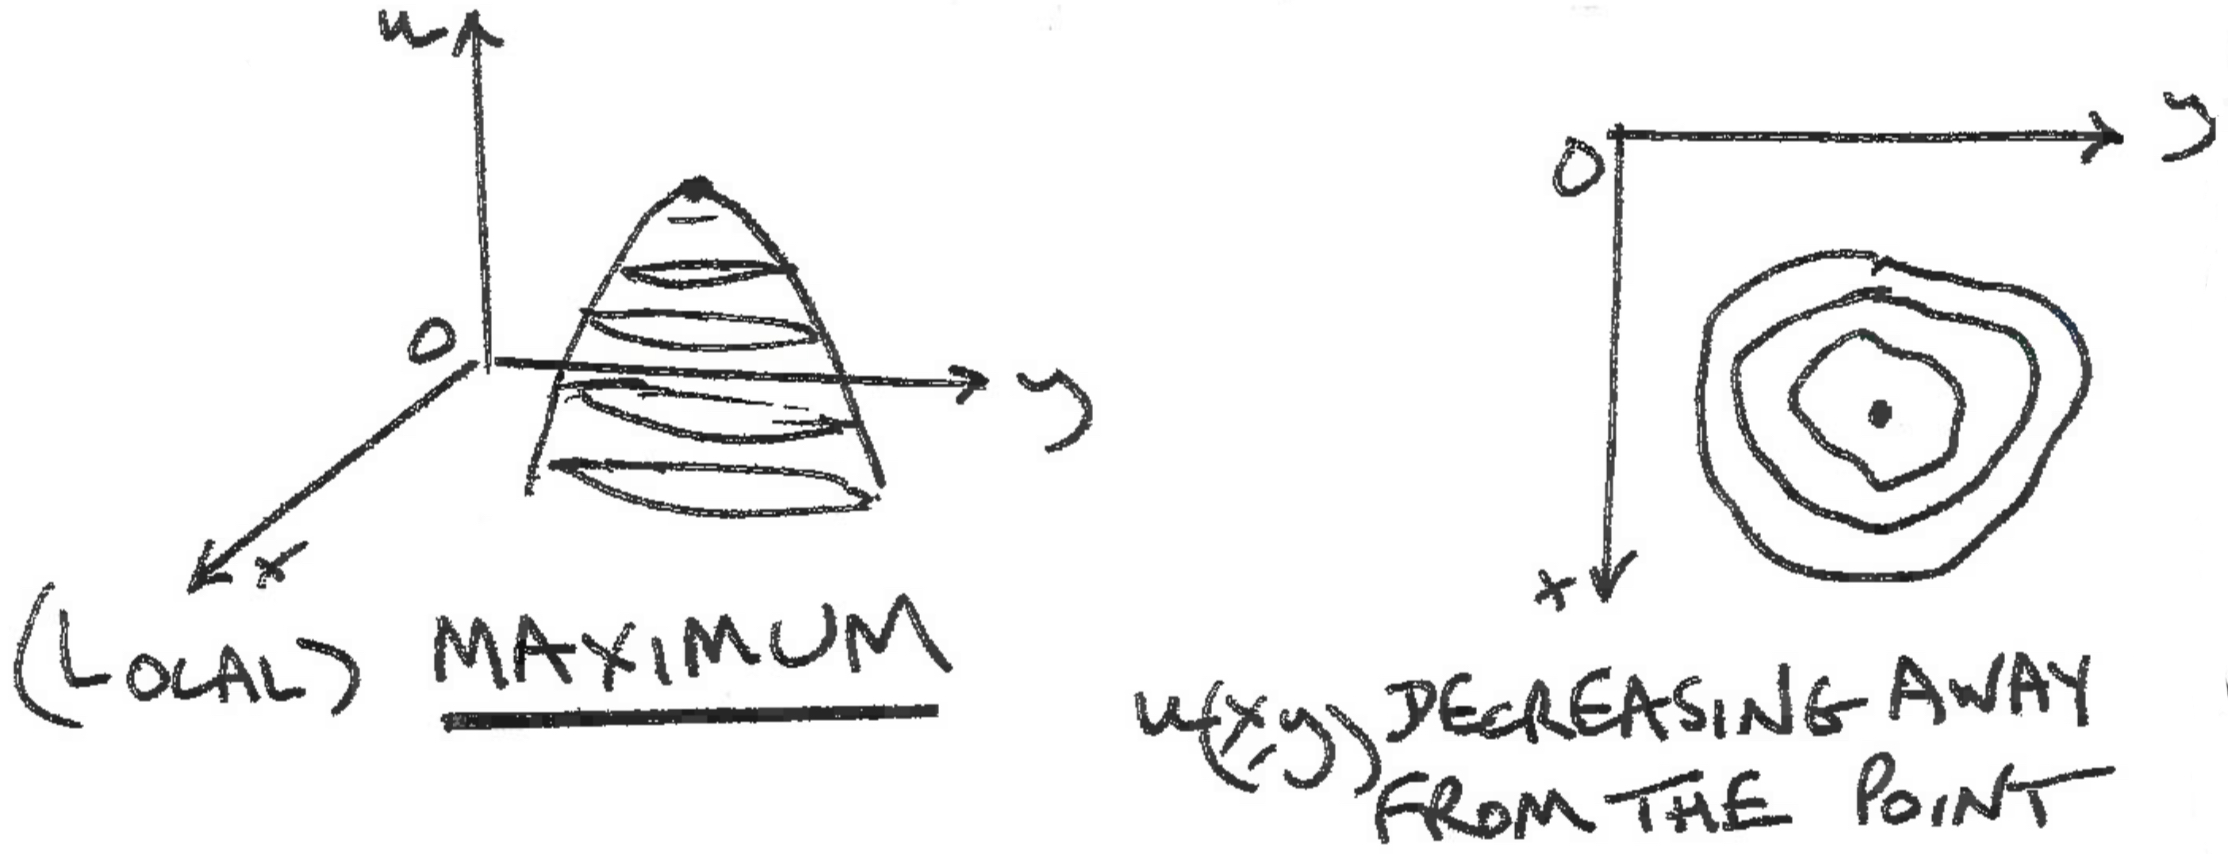
\includegraphics[scale=0.15]{localMaximum.jpeg}
  	\centering
    \caption{local maximum}\label{fig:localMax}
\end{figure}

\begin{figure}
  	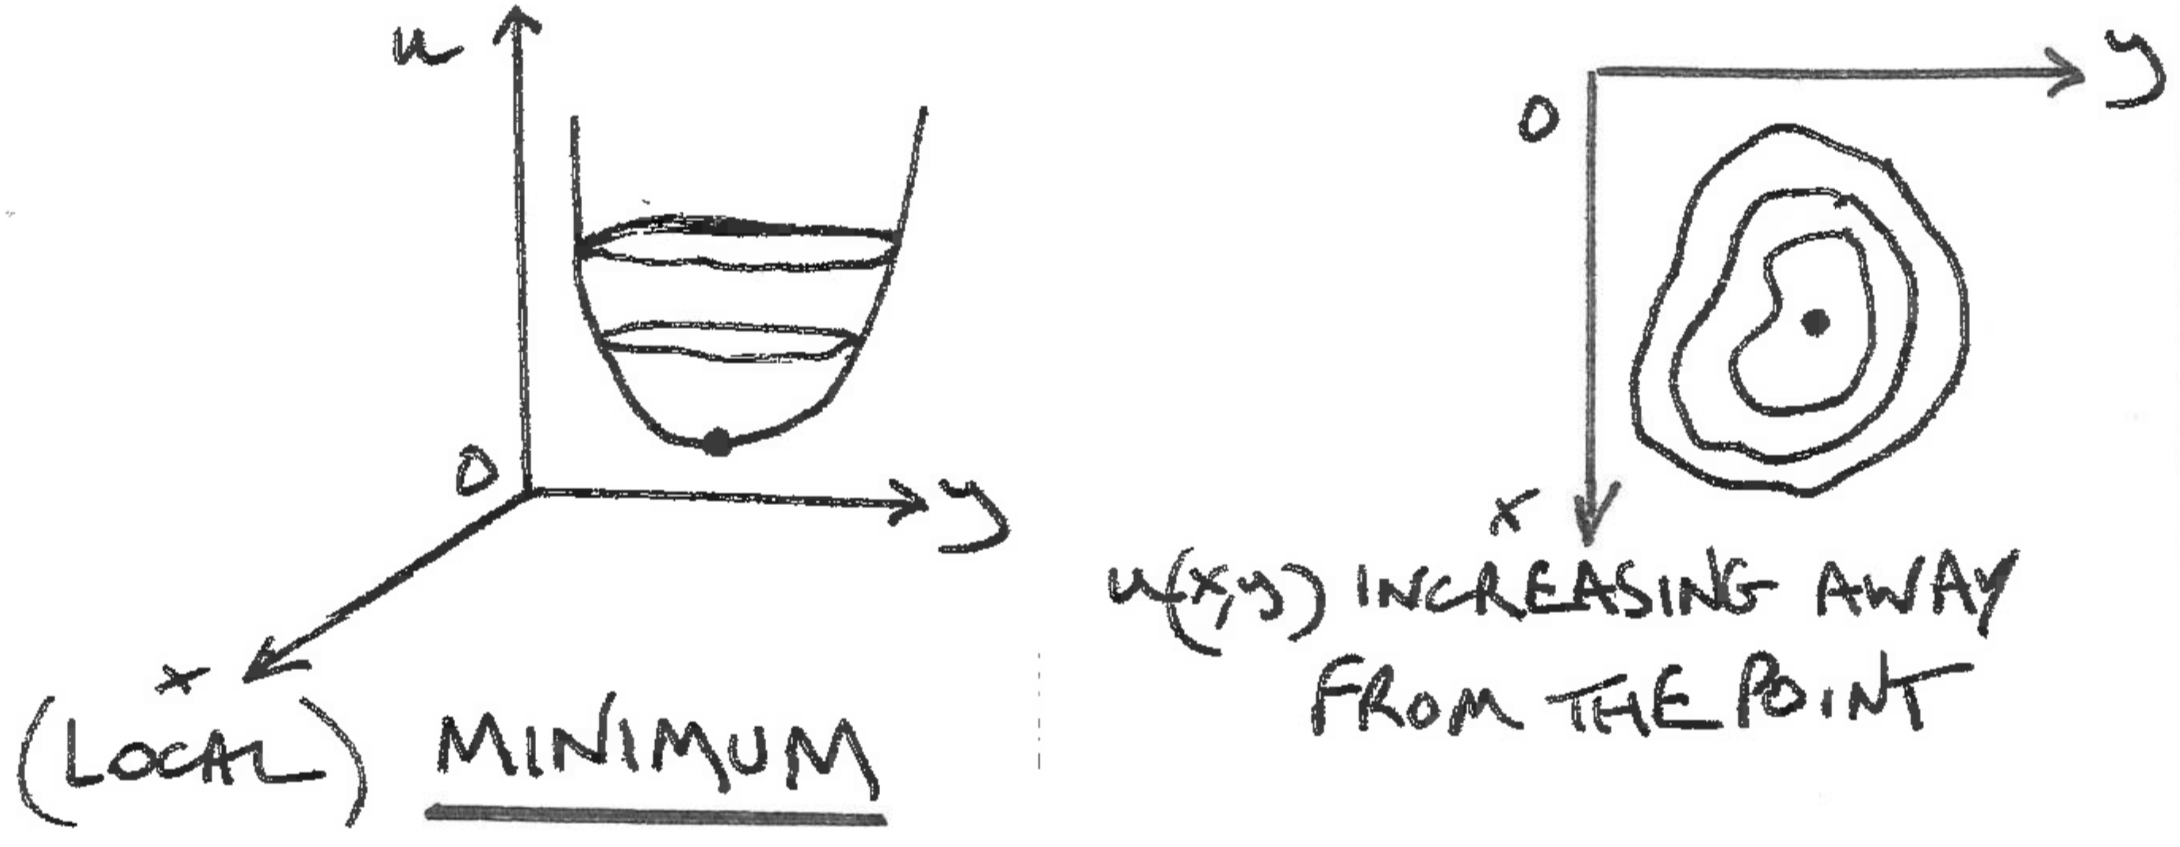
\includegraphics[scale=0.15]{localMinimum.jpeg}
  	\centering
    \caption{local minimum}\label{fig:localMin}
\end{figure}

\begin{figure}
  	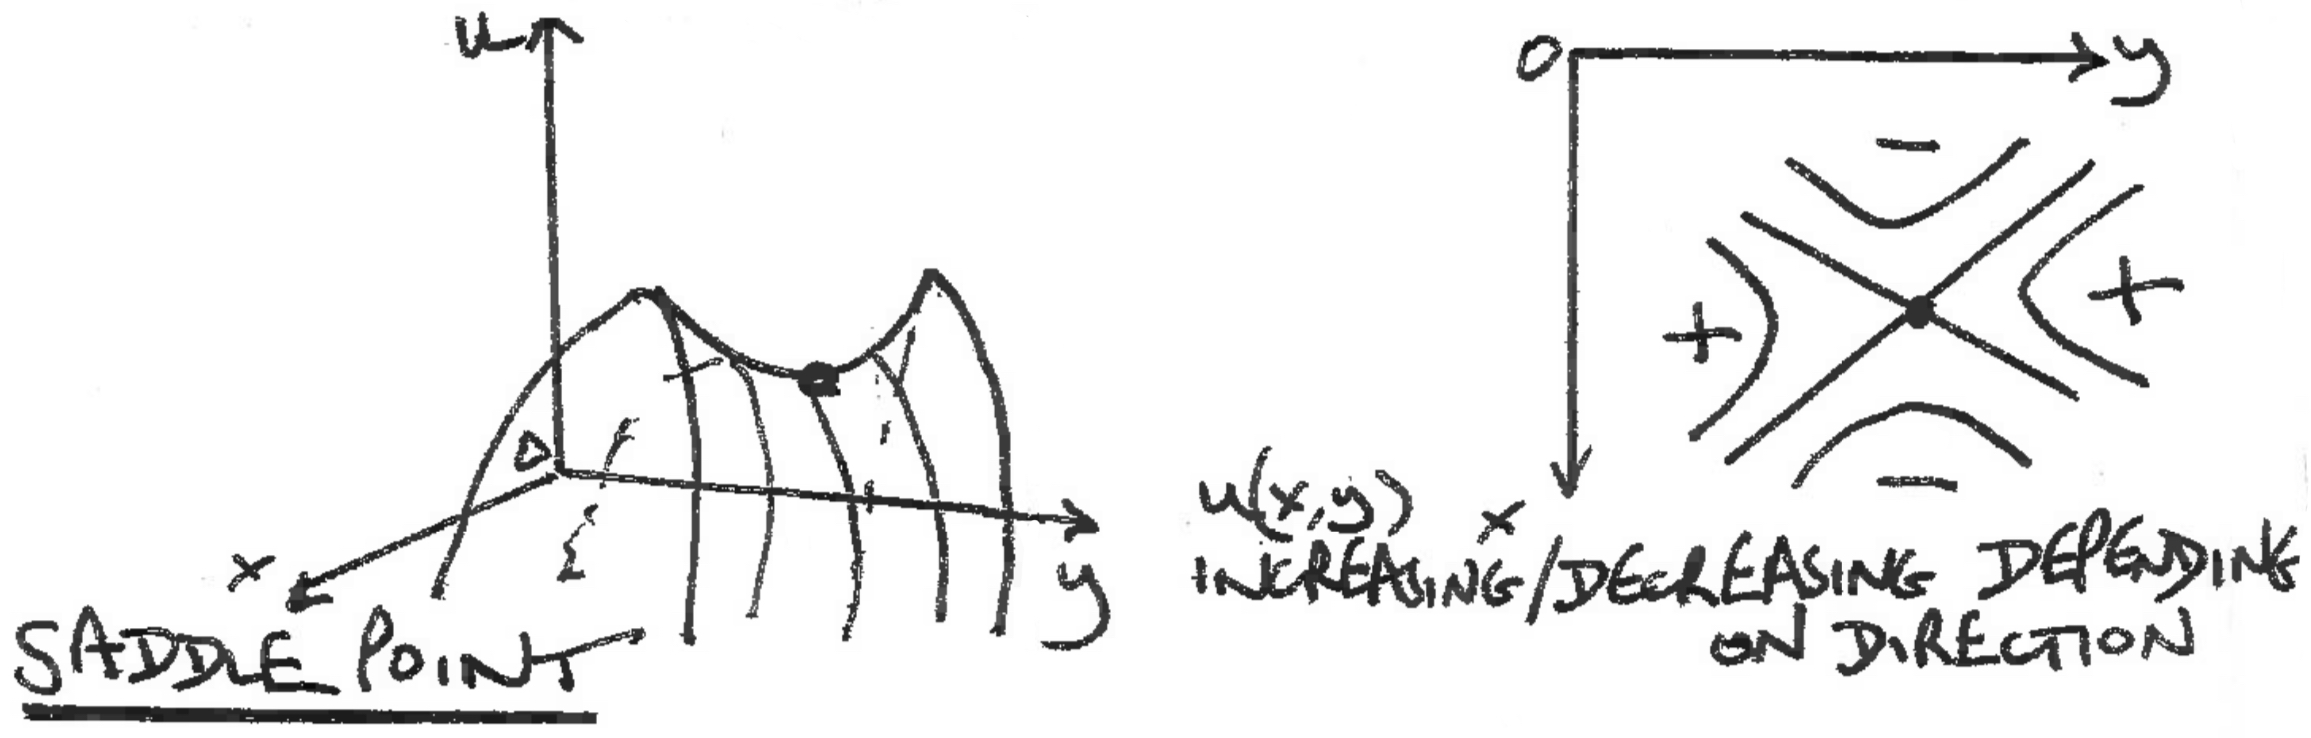
\includegraphics[scale=0.15]{saddlePoint.jpeg}
  	\centering
    \caption{saddle point}\label{fig:saddlePoint}
\end{figure}

How do we distinguish between these cases?

Consider a stationary point $(x_0,y_0)$ where we have (of course)
${\left(\frac{\partial u}{\partial x} \right)}_{0} = 0 = {\left(\frac{\partial u}{\partial y} \right)}_{0}$.
Then we write out the Taylor expansion for $u(x,y)$ about $(x_0, y_0)$
exactly as Equation~\eqref{PDE:1}. The first order terms are cancelled out, so\[
    \begin{align*}
        \delta u & = u(x_0 + h, y_0 + k) - u(x_0, y_0) \\
                 & = \frac{1}{2}\left[Ah^{2} + 2Bhk + Ck^{2}\right] + \cdots
    \end{align*}
\]where\[
    A = {\left(\frac{\partial^{2}u}{\partial x^{2}} \right)}_{0}, \quad
    B = {\left(\frac{\partial^{2}u}{\partial x \partial y} \right)}_{0}, \quad
    C = {\left(\frac{\partial^{2}u}{\partial y^{2}} \right)}_{0},
\]and $\delta u$ can be written in matrix form:\[
    \delta u = \frac{1}{2}\begin{pmatrix}
        h & k
    \end{pmatrix} \begin{pmatrix}
        A & B \\
        B & C
    \end{pmatrix} \begin{pmatrix}
            h \\
            k
    \end{pmatrix} + \cdots.
\]
\underline{Note}: If $A, B, C$ are all $0$, then we need higher-order terms.

\bigskip
As such,
\begin{enumerate}[label = (\roman*)]
    \item $\delta u > 0$ for \emph{any} small $h,k$ then $u(x_0,y_0)$ is a (local) minimum.
    \item $\delta u < 0$ for \emph{any} small $h,k$ then $u(x_0, y_0)$ is a (local) maximum.
    \item $\delta u$ can be positive or negative depending on the value of $h, k$,
        then $u(x_0,y_0)$ is a saddle point.
\end{enumerate}

The easiest way to determine this is via e.g.\[
    \delta u = \frac{1}{2}k^{2}\left[A{\left(\frac{h}{k}\right)}^{2} 
    + 2B\left(\frac{h}{k}\right) + C\right] + \cdots
\]and consider\[
F(\lambda) = A\lambda^{2} + 2B\lambda + C.
\]

(Possible to think in terms of $B^{2}-AC$, as this is more ``natural''
while thinking about \emph{discriminant} of polynomials. Then
all the following deductions/conclusions should be reversed!)

\begin{figure}
  	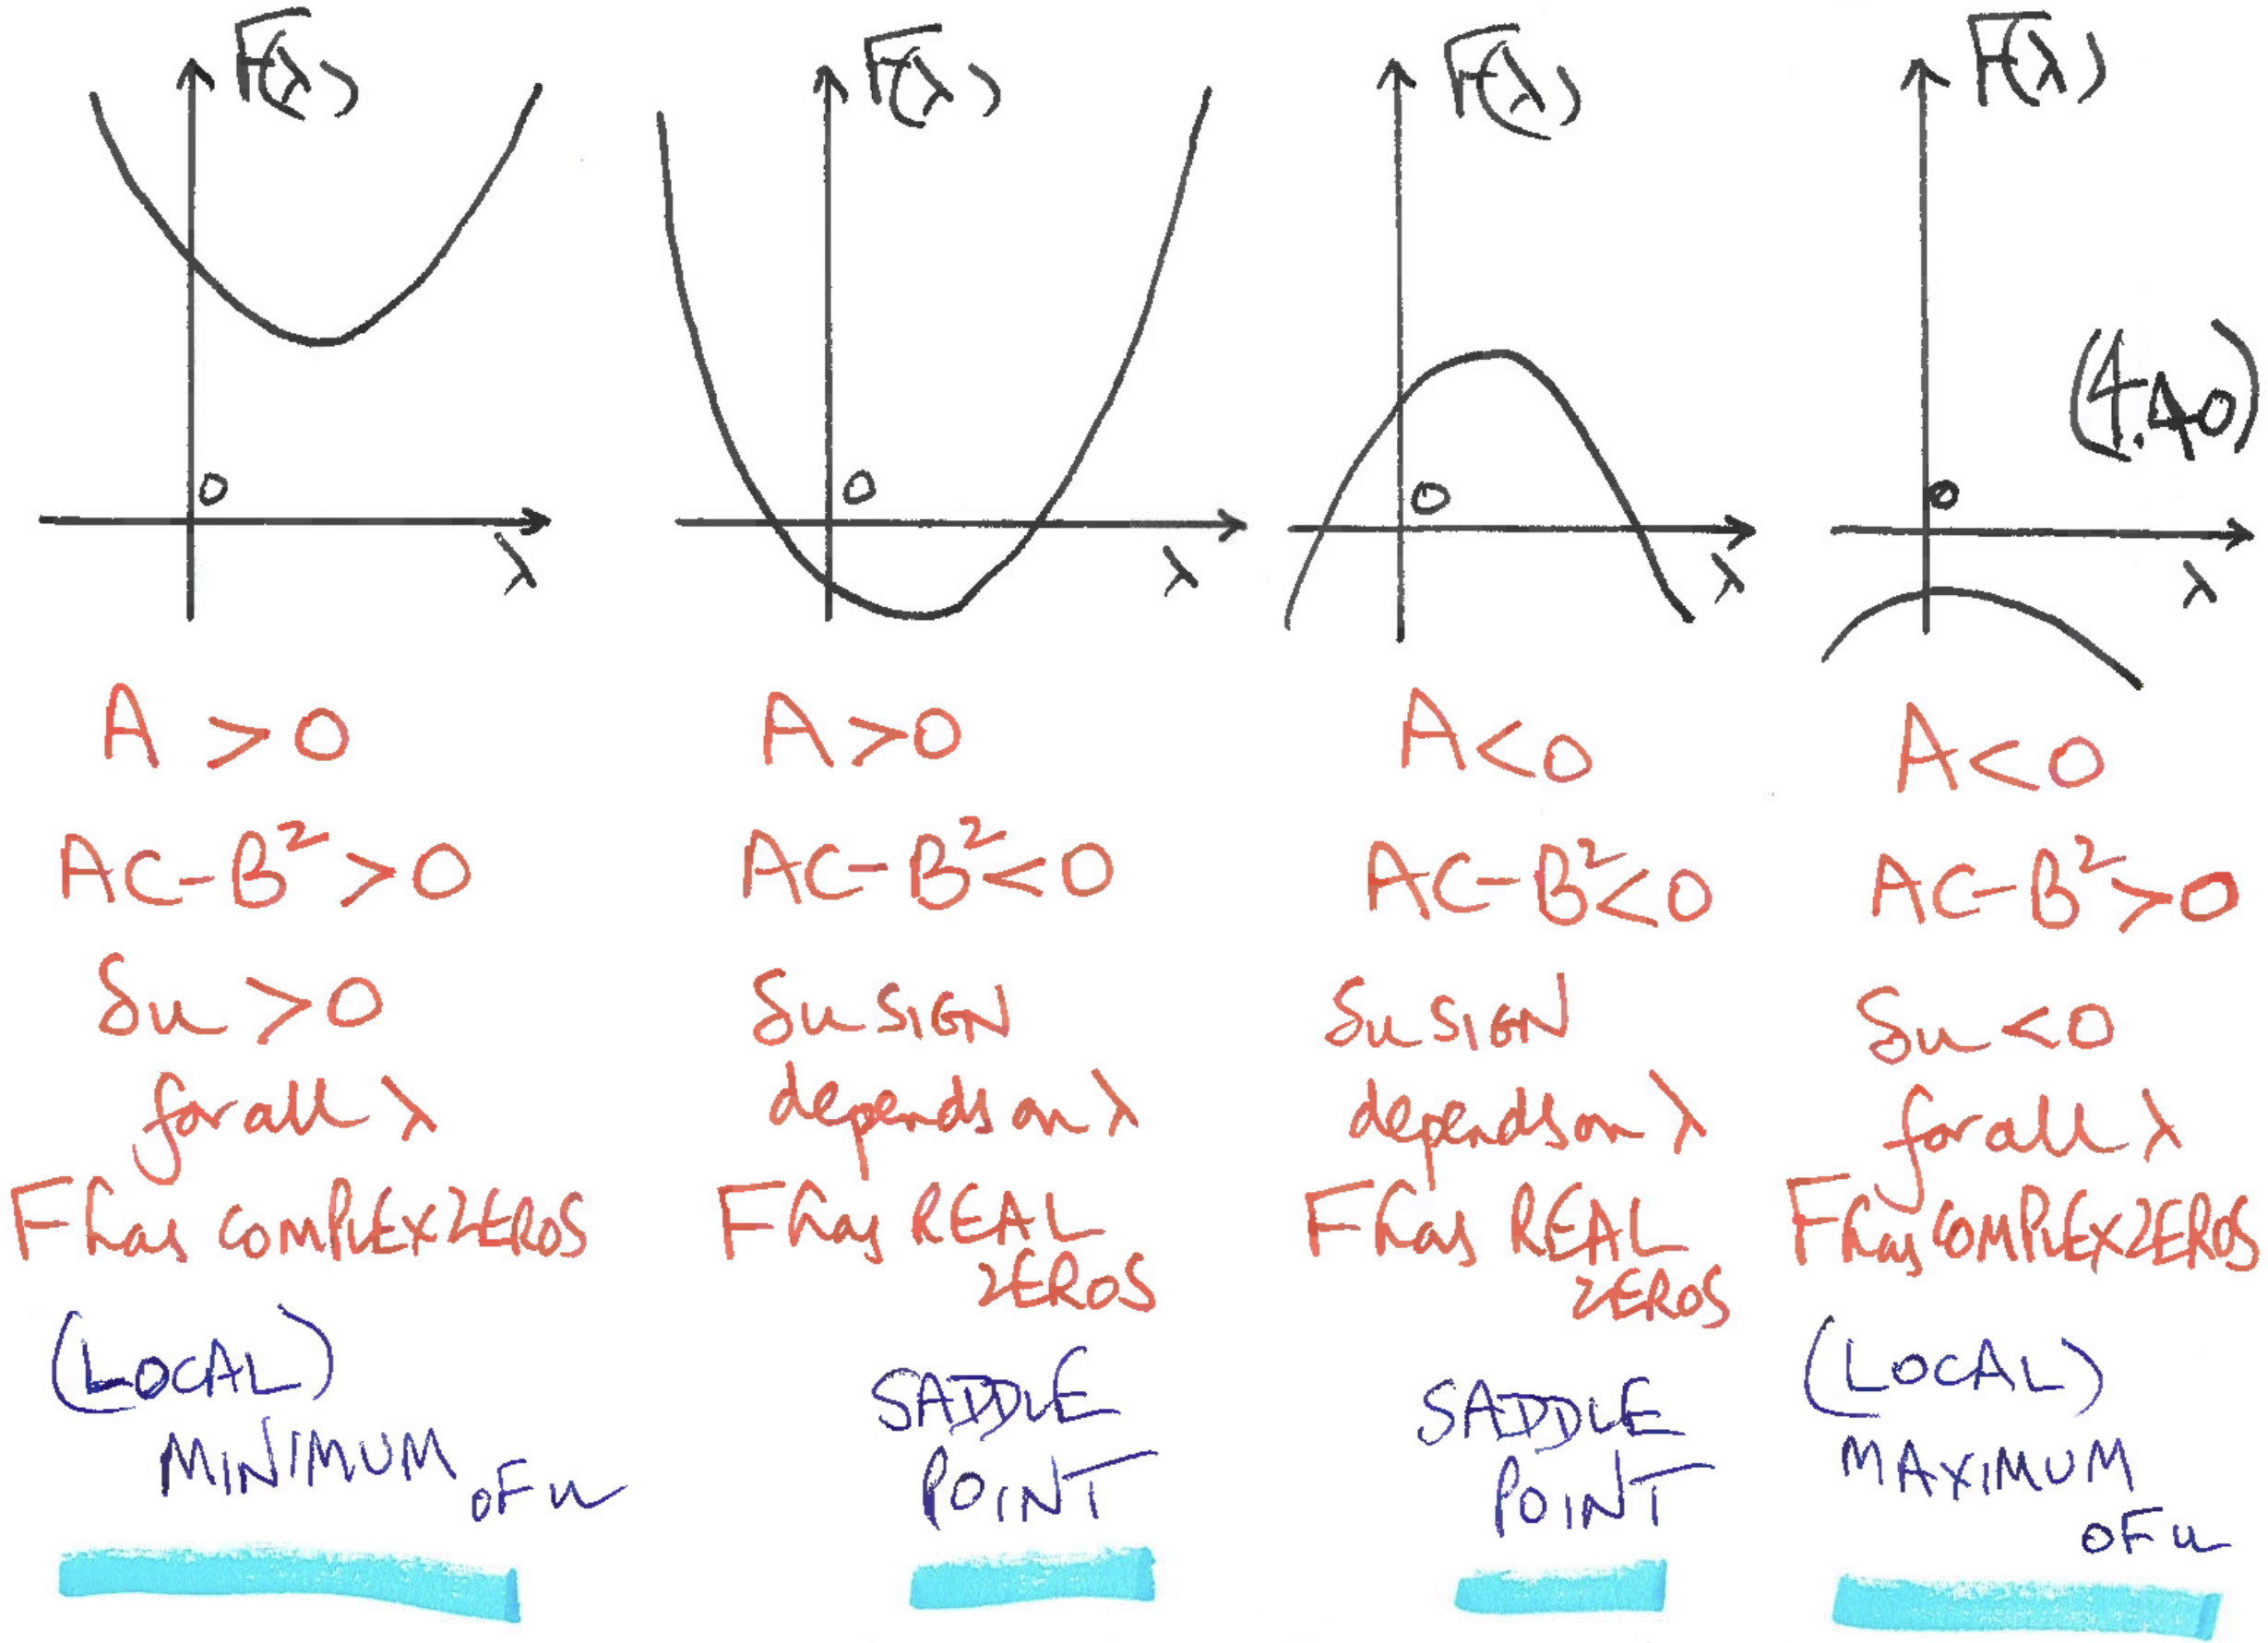
\includegraphics[scale=0.15]{stationaryPointDet.jpeg}
  	\centering
    \caption{graphs to determine what type of stationary point it is}\label{fig:stationaryPointDet}
\end{figure}

\paragraph{Summary}

For functions of two variables $u(x,y)$, stationary points are located at simultaneous solution
of the two equations:\[
    \left\{\begin{align*}
        & \frac{\partial u}{\partial x} = 0 \\
        & \frac{\partial u}{\partial y} = 0
    \end{align*}\right.
\]where $\mathrm{d}u = 0$ locally.
Each $(x_0, y_0)$ has \emph{character} determined by\[
    E_0 = {\left[\left(\frac{\partial^{2}u}{\partial x^{2}} \right)
    \left(\frac{\partial^{2}u}{\partial y^{2}} \right)
    - {\left(\frac{\partial^{2}u}{\partial x\partial y} \right)}^{2}\right]}_{0} = AC-B^{2}
\]with
\begin{itemize}
    \item $E_0 < 0$ implies a saddle point,
    \item $E_0 > 0$ and
        \begin{itemize}
            \item ${\left(\frac{\partial^{2}u}{\partial x^{2}} \right)}_{0} < 0$ implies a (local) maximum,
            \item ${\left(\frac{\partial^{2}u}{\partial x^{2}} \right)}_{0} > 0$ implies a (local) minimum.
        \end{itemize}
\end{itemize}
Of course there are \emph{singular} cases that can occur, such as
$E_0 = 0, A = B = C = 0$ etc.
These normally require higher-order derivatives to determine the issue --- not considered here.

\paragraph{Examples}
\,

\begin{enumerate}[label = (\roman*)]
    \item $u(x,y) = x^{3} + xy^{2} - x - yx^{2} - y^{3} + y = (x-y)(x^{2}+y^{2}-1)$.
        \[
            \Rightarrow{}\left\{\begin{align*}
                    \frac{\partial u}{\partial x} & = 3x^{2} + y^{2} - 1 - 2xy = 0 \\
                    \frac{\partial u}{\partial y} & = 2xy - x^{2} - 3y^{2} + 1 = 0.
            \end{align*}\right.
        \]By adding the two equations up, we get $2x^{2}-2y^{2}=0, y = \pm x$.
        When $y = x$, $x = \pm \frac{1}{\sqrt{2}}$; when $y = -x$, $x = \pm \frac{1}{\sqrt{6}}$.
        Thus there are four stationary points:\[
            P_1\left(\frac{1}{\sqrt{2}}, \frac{1}{\sqrt{2}}\right),
            P_2\left(-\frac{1}{\sqrt{2}}, -\frac{1}{\sqrt{2}}\right),
            P_3\left(\frac{1}{\sqrt{6}}, -\frac{1}{\sqrt{6}}\right),
            P_4\left(-\frac{1}{\sqrt{6}}, \frac{1}{\sqrt{6}}\right).
        \]
        Then we can analyse the stationary points,
        as shown in Figure~\ref{fig:stationaryPointsAnalysis},
        and sketch the contours, as shown in Figure~\ref{fig:contourSketch}!

\begin{figure}
  	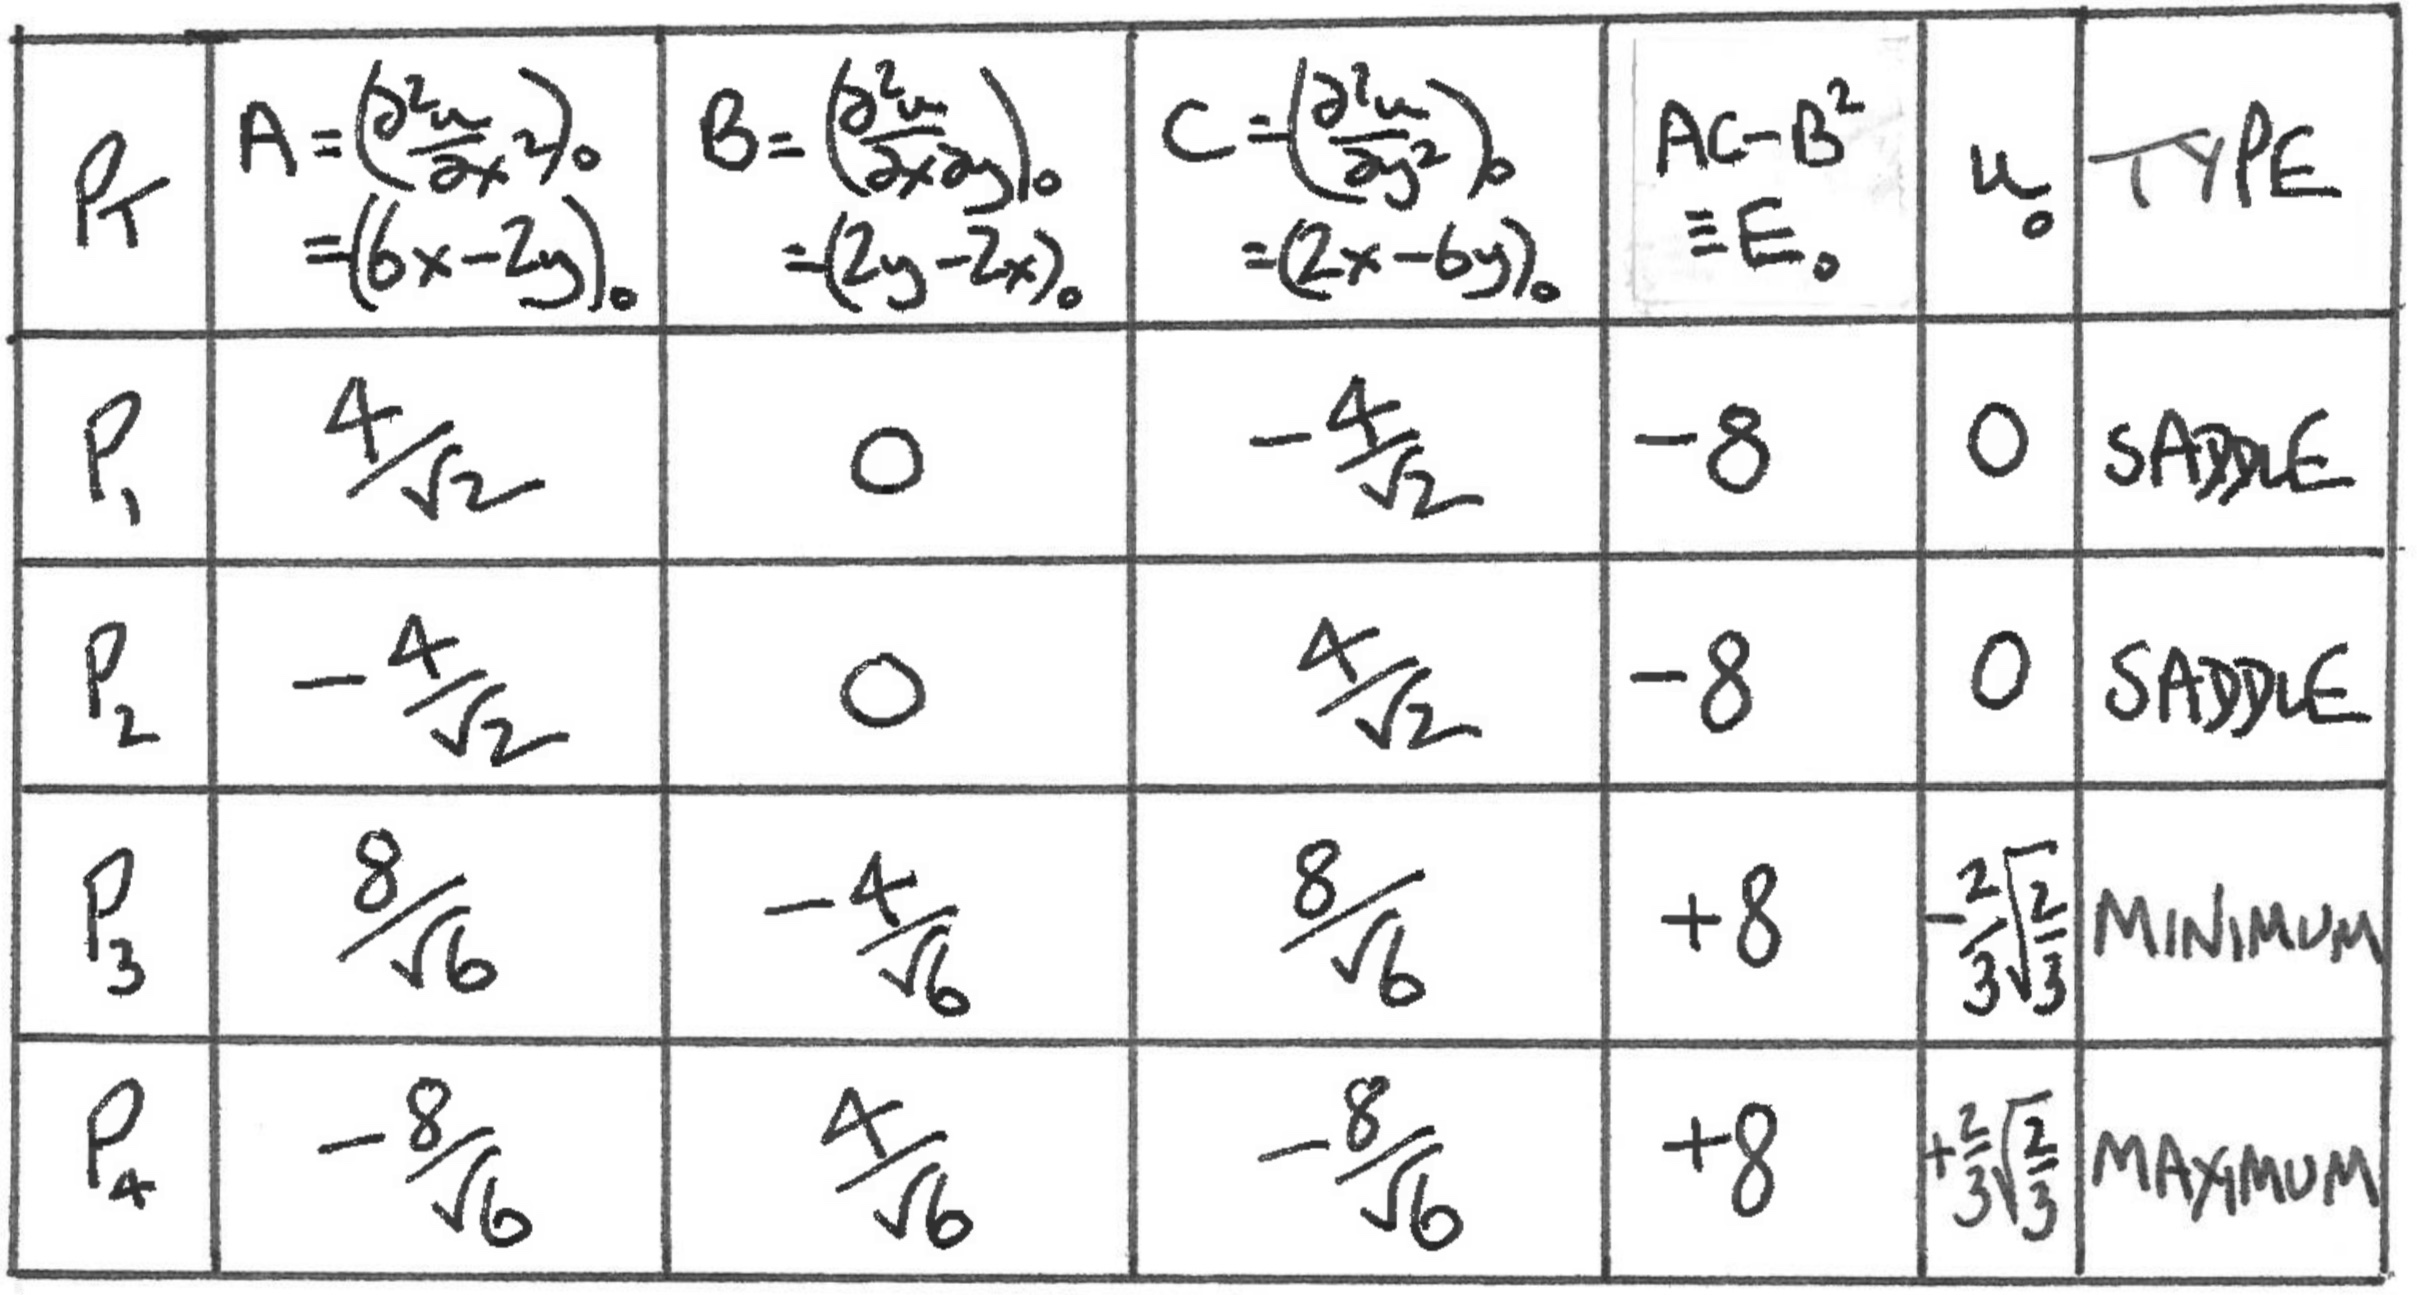
\includegraphics[scale=0.15]{stationaryPointsAnalysis.jpg}
  	\centering
    \caption{stationary points analysis}\label{fig:stationaryPointsAnalysis}
\end{figure}

\begin{figure}
  	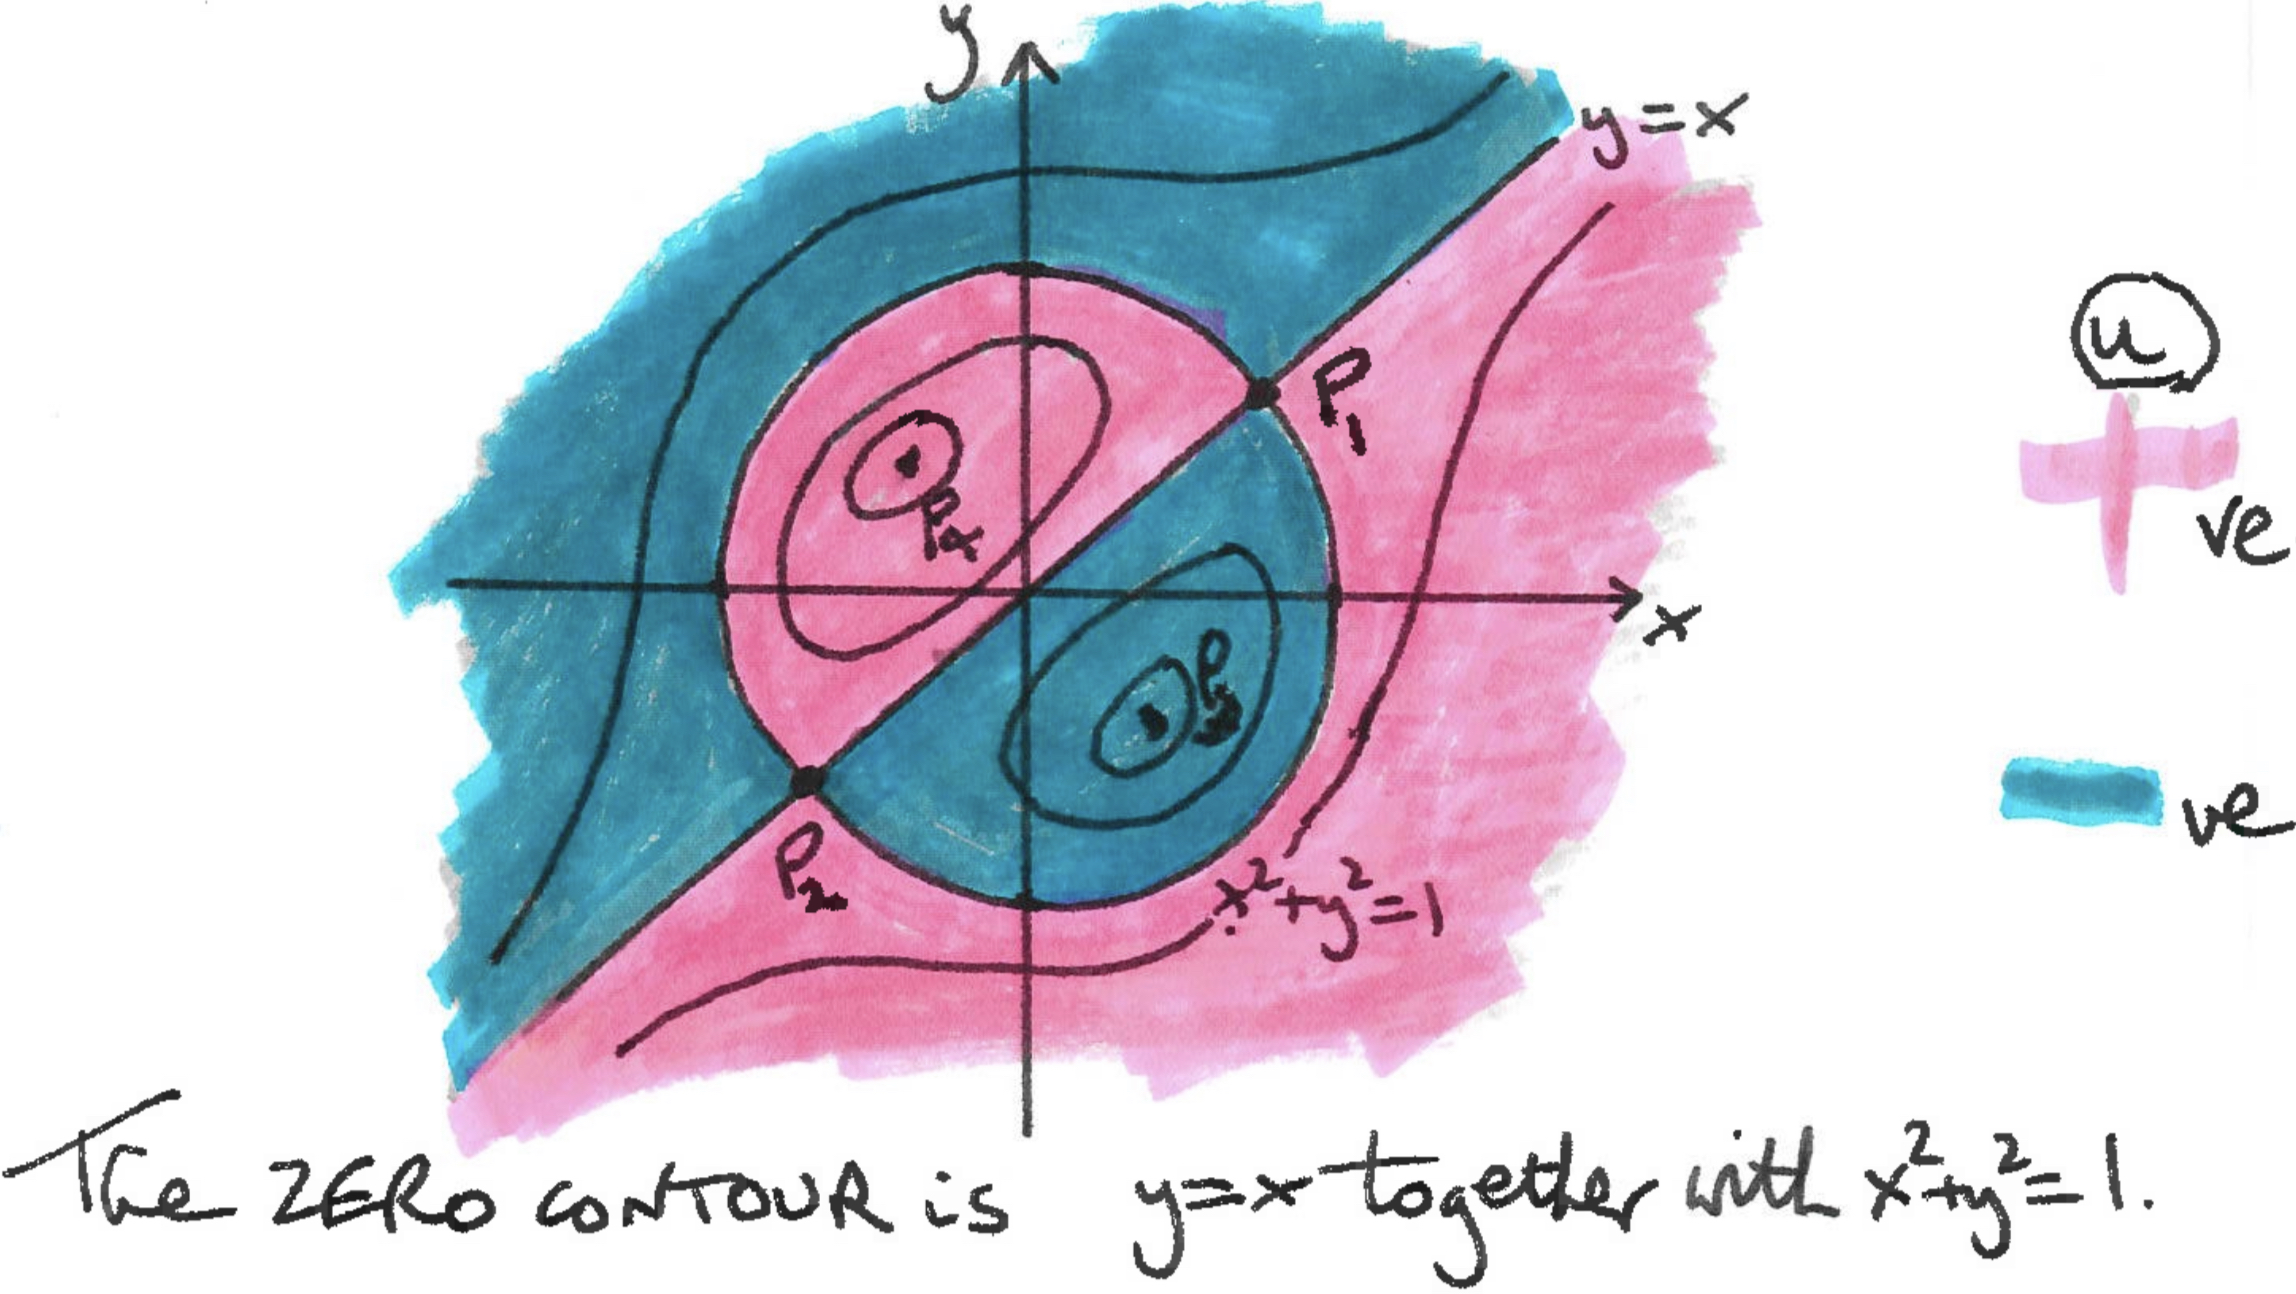
\includegraphics[scale=0.15]{contourSketch.jpeg}
  	\centering
    \caption{contour sketch}\label{fig:contourSketch}
\end{figure}


        \underline{Warning}:
        When we are faced with a function of several variables and we need to find stationary points 
        (and potential local max and min), we need to ensure that our \emph{independent} variables 
        are indeed independent.

    \item Maximise volume $V = xyz$ of a rectangular box given the surface area 
        $A = 2xy + 2yz + 2zx$ is fixed.
        In this case, $x, y, z$ are \emph{not} independent.
        We then need to write\[
            z = \frac{A - 2xy}{2(x+y)} \Rightarrow{}
            V = \frac{xy(A-2xy)}{2(x+y)}.
        \]Now $x, y$ are independent, so we can solve and derive that\[
        x_0 = \sqrt{\frac{A}{6}} = y_0 (= z_0), V_{\max} = {\left(\frac{A}{6}\right)}^{\frac{3}{2}}.
        \]
\end{enumerate}

\subsection{Application --- Exact (First Order) Differential Equations}

We know that for a function of two variables $u(x,y)$ the total differential is\[
    \mathrm{d}u = \frac{\partial u}{\partial x} \mathrm{d}x + \frac{\partial u}{\partial y} \mathrm{d}y
\]and of course $\frac{\partial u}{\partial x} $ and $\frac{\partial u}{\partial y} $
will both, in general, be functions of $x$ and $y$.
Now consider the converse problem! Given \[
    P(x,y)\mathrm{d}x + Q(x,y)\mathrm{d}y
\]i.e.\ given $P$ and $Q$, when is it the case that this \emph{is}
the total differential of some (as yet unknown) function $u(x,y)$?
If it is such then $P(x,y) = \frac{\partial u}{\partial x} $ and $Q(x,y) = \frac{\partial u}{\partial y} $
for that function $u(x,y)$.
This implies (easy!) and is implied by (proof not given here!) the 
\emph{\underline{condition of integrability}}:\[
    \frac{\partial P}{\partial y} = \frac{\partial Q}{\partial x}.
\]

\paragraph{Examples}
\,

\begin{enumerate}[label = (\roman*)]
    \item $y^{2}\mathrm{d}x + (x^{2}+2y)\mathrm{d}y$.
        Since\[
            \frac{\partial P}{\partial y} = 2y
            \not\equiv \frac{\partial Q}{\partial x} = 2x,
        \]the test fails, and thus not an exact/total differential.

    \item $(2xy + \cos{x}\cos{y})\mathrm{d}x + (x^{2}-\sin{x}\sin{y})\mathrm{d}y$.
        \[
            \frac{\partial P}{\partial y} = 2x - \cos{x}\sin{y} = \frac{\partial Q}{\partial x},
        \]so the test pass and it is exact. Thus\[
        \frac{\partial u}{\partial x} = 2xy + \cos{x}\cos{y}
        \]\[
        \Rightarrow{}u(x,y) = x^{2}y + \sin{x}\cos{y} + f(y)
    \]where $f(y)$ is a `constant' of integration w.r.t. $x$.
    Then either\[
        \begin{align*}
            \frac{\partial u}{\partial y} 
            & = x^{2} - \sin{x}\sin{y} + \frac{\mathrm{d}f(y)}{\mathrm{d}y} \\
            & = x^{2} - \sin{x}\sin{y}
        \end{align*}
    \]so that $\frac{\mathrm{d}f}{\mathrm{d}y} = 0$ and $f(y) = K$ constant w.r.t. $x$ and $y$,
    or alternatively\[
        \frac{\partial u}{\partial y} = x^{2}-\sin{x}\sin{y}
    \]\[
    \Rightarrow{}u(x,y) = x^{2}y + \sin{x}\cos{y} + g(x)
\]where $g(x)$ is the `constant' of integration w.r.t. $y$.
Comparing the two expressions and deduce that $f(y) = g(x) = K$ constant
independent of $x$ and $y$. This also gives\[
    u(x,y) = x^{2}y + \sin{x}\cos{y} + K
\]and $P\mathrm{d}x + Q\mathrm{d}y = \mathrm{d}u(x,y)$.
\end{enumerate}

\bigskip
Now consider an equation of the form
\begin{equation}\label{eqn:9}
    P(x,y)\mathrm{d}x + Q(x,y)\mathrm{d}y = 0.
\end{equation}
This is a first order differential equation, with alternative forms
$\frac{\mathrm{d}y}{\mathrm{d}x} = -\frac{P(x,y)}{Q(x,y)}$ and $P + Q\frac{\mathrm{d}y}{\mathrm{d}x} = 0$.
If $P\mathrm{d}x + Q\mathrm{d}y$ is the total differential of a function $u(x,y)$,
i.e.\ $\mathrm{d}u(x,y) = 0$,
then the solution is \[
    u(x,y) = \;\textnormal{constant}\;C.
\]In this case~\eqref{eqn:9} is an \textbf{\emph{exact differential equation}}.  
From the example (ii) above,\[
    (2xy + \cos{x}\cos{y})\mathrm{d}x + (x^{2} - \sin{x}\sin{y})\mathrm{d}y = 0
\]has solution\[
u(x,y) = x^{2}y + \sin{x}\cos{y} = C.
\]
What if $P\mathrm{d}x + Q\mathrm{d}y$ is not exact, which would mean that%
~\eqref{eqn:9} would not be an exact differential equation?
We can consider multiplying through by a factor $\lambda(x,y)$,\[
    \Rightarrow{}(\lambda P)\mathrm{d}x + (\lambda Q)\mathrm{d}y = 0
\]which is the `same' differntial equation as~\eqref{eqn:9},
but can we make it exact? Evidently we would need
\begin{equation}\label{eqn:10}
    \frac{\partial}{\partial y} (\lambda P) = \frac{\partial}{\partial x} (\lambda Q)
\end{equation}
\[
    \Rightarrow{}P\frac{\partial \lambda}{\partial y} - Q\frac{\partial \lambda}{\partial x} 
    + \lambda\left(\frac{\partial P}{\partial y} - \frac{\partial Q}{\partial x} \right) = 0.
\]
This is a \emph{partial} differential equation for $\lambda$ given $P, Q$.
It can be shown that there is a solution, but
this isn't normally very helpful in finding it!
However, sometimes we can find a suitable $\lambda$ by \emph{\underline{inspection}}!

\paragraph{Example}
\begin{enumerate}[label = (\arabic*)]
    \item 
\[
    (xy-1)\mathrm{d}x + (x^{2}-xy)\mathrm{d}y = 0
\]\[
    \Rightarrow{}\frac{\partial P}{\partial y} = x 
    \not\equiv \frac{\partial Q}{\partial x} = 2x-y.
\]
Let's \emph{try} $\lambda(x)$ (with $x$ only) say and use~\eqref{eqn:10},\[
    \Rightarrow{} \lambda(x)x = \frac{\mathrm{d}\lambda(x)}{\mathrm{d}x} (x^{2}-xy) + \lambda(x)(2x-y)
\]($\frac{\mathrm{d}\lambda(x)}{\mathrm{d}y} = 0$) so that 
$\frac{1}{\lambda} \frac{\mathrm{d}\lambda}{\mathrm{d}x} = -\frac{1}{x}$, 
$\lambda = \frac{K}{x}$,
and we can take $K = 1$ W.L.O.G.\[
\Rightarrow{}(y-\frac{1}{x})\mathrm{d}x + (x-y)\mathrm{d}y = 0 \quad\;\textnormal{is exact!}\;
\]\[
\Rightarrow{}u(x,y) = xy - \ln{|x|} - \frac{1}{2}y^{2} - C,
\]\[
xy - \ln{|x|} - \frac{1}{2}y^{2} = C
\]is the general solution of our equation.

\item \[
        \frac{\mathrm{d}y}{\mathrm{d}x} + f(x)y = g(x)
\]\[
\Rightarrow{}[yf(x) - g(x)]\mathrm{d}x + \mathrm{d}y = 0
\]and $\frac{\partial}{\partial y} (yF-G) = F \not\equiv \frac{\partial}{\partial x} (1) = 0$ in general.
Try integrating factor $\lambda(x)$ only:\[
    \frac{1}{\lambda} \frac{\mathrm{d} \lambda}{\mathrm{d}x} = f(x)
    \Rightarrow{}\lambda = K \exp{\left[\int_{}^{x} f(x)\mathrm{d}x\right]}.
\]
So the term \emph{integrating factor} has the same meaning, as in the previous chapter!
\end{enumerate}

\subsection{Application --- Vector Calculus}

We often need to consider \emph{scalar} and \emph{vector} functions of position
$\mathbf{r} (= x\mathbf{i} + y\mathbf{j} + z\mathbf{k})$ (\emph{fields}): 
$\phi(\mathbf{r})$ and $\mathbf{u}(\mathbf{r}) = u_1\mathbf{i} + u_2\mathbf{j} + u_3\mathbf{k}$.
These could represent e.g.\ the temperature ($\phi$) and velocity ($\mathbf{u}$) within a material.
Of course they might also practically depend on time $t$ too, but for now
we consider \emph{spatial} rates of change.

\newmdtheoremenv[style=defEnv]{partial differential operator}[theorem]{Definition}
\begin{partial differential operator}
The \textbf{\emph{partial differential operator}} is defined as\[
    \nabla \equiv \mathbf{i}\frac{\partial}{\partial x} + \mathbf{j}\frac{\partial}{\partial y} + \mathbf{k}\frac{\partial}{\partial z}
\]
\end{partial differential operator}

There are 3 important derived fields, each involving the (partial) differential operator. They are:
\begin{enumerate}[label = (\arabic*)]
    \item 
        \[
            \nabla \phi = \mathbf{i}\frac{\partial\phi}{\partial x}
            + \mathbf{j}\frac{\partial\phi}{\partial y} + \mathbf{k}\frac{\partial\phi}{\partial z}
            \equiv \;\textnormal{grad}\;\phi \quad\;\textnormal{`Gradient'}\;
        \]which is a vector field.
        It is measuring \emph{the rate of change of a value in each dimension}.
        
    \item 
        \[
            \nabla \cdot \mathbf{u} = \frac{\partial u_1}{\partial x} 
            + \frac{\partial u_2}{\partial y} + \frac{\partial u_3}{\partial z}
            \equiv \;\textnormal{div}\;\mathbf{u} \quad\;\textnormal{`Divergence'}\;
        \]which is a scalar field.
        It is measuring \emph{the overall rate of change of a vector in each standard basis}
        by decomposing the vector into its corresponding dimensions
        and summing up the rate of change of each component.

    \item 
        \[
            \nabla \times \mathbf{u} = \mathbf{i}\left(\frac{\partial u_3}{\partial y}
            - \frac{\partial u_2}{\partial z}\right)
            + \mathbf{j}\left(\frac{\partial u_1}{\partial z} - \frac{\partial u_3}{\partial x}\right)
            + \mathbf{k}\left(\frac{\partial u_2}{\partial x} - \frac{\partial u_1}{\partial y}\right)
            \equiv \;\textnormal{curl}\;\mathbf{u}
        \]which is a vector field.
        It is measuring \emph{the rate of rotation/curl about a point},
        hence the output is a vector field with vectors describing the
        direction and magnitude of rotation about each point.
        The expression can be `mnemonically' memorized in the following form:\[
            \det{\begin{pmatrix}
                    \mathbf{i} & \mathbf{j} & \mathbf{k} \\
                    \frac{\partial}{\partial x} & \frac{\partial}{\partial y} & \frac{\partial}{\partial z} \\
                    u_1 & u_2 & u_3
            \end{pmatrix} }
        \]
\end{enumerate}

Each of these fields has a strong physical meaning and can be interpreted in
e.g. 2 dimensions $(x,y)$ if required.

\begin{enumerate}[label = (\arabic*)]
    \item $\nabla\phi\equiv$ grad $\phi$.

        At each point $\nabla\phi$ is \emph{perpendicular} to the $\phi =$ constant surface through the point.
        If $\mathrm{d}\mathbf{r} = \mathrm{d}x\mathbf{i}
        + \mathrm{d}y\mathbf{j} + \mathrm{d}z\mathbf{k}$
        along the surface at $P$, then\[
            (\nabla\phi)\cdot\mathrm{d}\mathbf{r} = 
            \frac{\partial\phi}{\partial x}\mathrm{d}x + \frac{\partial\phi}{\partial y}\mathrm{d}y
            + \frac{\partial\phi}{\partial z}\mathrm{d}z = \mathrm{d}\phi = 0
        \]because $\phi = \phi_1$ on that surface through $P$.
        We note that $\nabla\phi$ is directed towards increasing $\phi$.

        \medskip
        \underline{Example}: 

        \begin{enumerate}[label = (\alph*)]
            \item $\phi = x^{2}y + 2xz$.
                \[
                    \begin{align*}
                        \nabla\phi & = (2xy + 2z, x^{2}, 2x) \\
                                   & = (-2, 4, 4)
                    \end{align*}
                \]at $P$ where $P(2, -2, 3)$.
                Unit normal to surface at $P = \pm \frac{-2\mathbf{i} + 4\mathbf{j} + 4\mathbf{k}}{\sqrt{36}}$.
    
                The rate of change of $\phi$ in a given direction $\hat{\mathbf{a}}$
                is given by\[
                    \nabla\phi\cdot\hat{\mathbf{a}} \equiv |\nabla\phi|\cos{\alpha}
                \]where $\alpha$ is the angle between $\nabla\phi$ and $\hat{\mathbf{a}}$.
                
                It is a \textbf{\emph{directional derivative}}.
                We can use $\nabla\phi$ to find rates of change, normals to curves and surfaces, tangent planes, \ldots
    
            \item $2xz^{2} - 3xy - 4x - 7 = 0$ (an equation about a surface).

                The normal to the surface at $(1, -1, 2)$ is\[
                    (2z^{2}-3y-4, -3x, 4xz) = 7\mathbf{i} - 3\mathbf{j} + 8\mathbf{k}.
                \]
                Equation of the tangent plane is\[
                    (\mathbf{r} - \mathbf{r}_0)\cdot(7, -3, 8) = 0
                \]i.e.\ \[
                ((x, y, z) - (1, -1, 2))\cdot(7, -3, 8) = 0
                \]\[
                \Rightarrow{}7(x-1) - 3(y+1) + 8(z-2) = 0.
                \]
        \end{enumerate}
        
    \item $\nabla\cdot\mathbf{u} \equiv$ div $\mathbf{u}$.

        It acts as a measurement of whether a local field is a
        \emph{source} ($+$) `outflow' / \emph{sink} ($-$) `inflow'.
        In general, the divergence at a point $\mathbf{x}$ is
        the limit of the ratio of the flux through the surface
        over the volume enclosing $\mathbf{x}$ approaching 0.
        In three dimensional Cartesian coordinates, the divergence
        is defined to be the above scalar function.

        \underline{Example}:\[
            \begin{align*}
                \mathbf{u} & = \frac{C\mathbf{r}}{r^{3}} \\
                           & = \frac{C}{r^{2}} \hat{\mathbf{r}} \\
                           & = C \frac{x\mathbf{i}+y\mathbf{j}+z\mathbf{k}}
                           {{(x^{2}+y^{2}+z^{2})}^{\frac{3}{2}}}
            \end{align*}
        \]\[
            \Rightarrow{}\frac{\partial u_1}{\partial x} 
            = \frac{\partial}{\partial x}\frac{Cx}{{(x^{2}+y^{2}+z^{2})}^{\frac{3}{2}}}
            = C \frac{y^{2}+z^{2}-2x^{2}}{{(x^{2}+y^{2}+z^{2})}^{\frac{5}{2}}}
        \]and two similar expressions.We can then derive that\[
            \nabla\cdot\mathbf{u}=\frac{\partial u_1}{\partial x}
            + \frac{\partial u_2}{\partial y} + \frac{\partial u_3}{\partial z} = 0
        \]except at $\mathbf{r} = 0$, where $\nabla\cdot\mathbf{u}$ is infinite!
        
        Some physical examples (inverse square law) include:
        \begin{enumerate}[label = (\roman*)]
            \item gravitational field $C = -Gm$, where mass is the source of the field.
            \item fluid source $C = \frac{V}{4\pi}$, where $V$ is the volume per second injected.
        \end{enumerate}
        
    \item $\nabla\times\mathbf{u}\equiv$ curl $\mathbf{u}$.

        It acts as a local rotation.

        \underline{Example}:
        \begin{enumerate}[label = (\alph*)]
            \item $\mathbf{u} = \mathbf{w}\times \mathbf{r}
                = w\mathbf{k}\times(x\mathbf{i}+y\mathbf{j}+z\mathbf{k})
                = -wy\mathbf{i} + wx\mathbf{j}$.\[
                    \Rightarrow{}\nabla\times\mathbf{u} = 2w\mathbf{k} = 2\mathbf{w}.
                \]where $\mathbf{w}$ is a vector pointing upward
                out of the plane, describing the rate of rotation.

                This describes the solid rotation,
                as illustrated in Figure~\ref{fig:solidRotation},
                and it turns out the the curl of $\mathbf{u}$ 
                is twice the constant rotation rate $\mathbf{w}$.

                \begin{figure}
                  	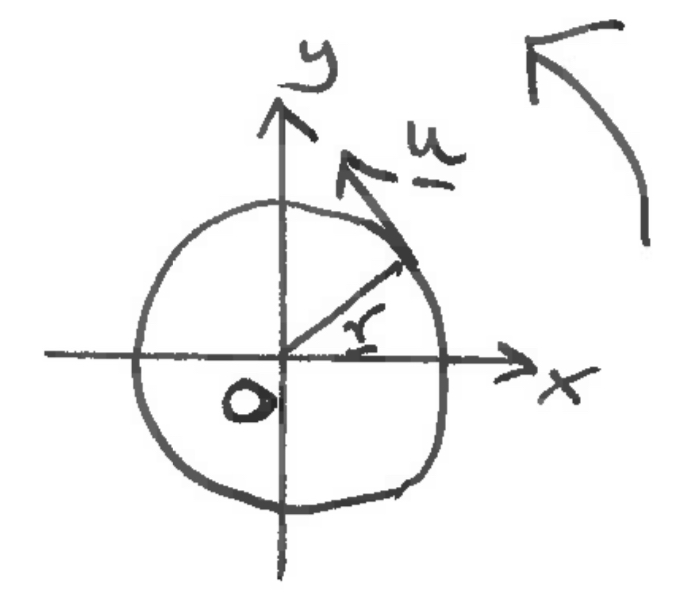
\includegraphics[scale=0.15]{solidRotation.jpeg}
                  	\centering
                    \caption{solid rotation illustration}\label{fig:solidRotation}
                \end{figure}
                

            \item $\mathbf{u} = (U+\alpha y, 0, 0)$

                This describes uniform shear flow,
                as illustrated in Figure~\ref{fig:shearFlow}.
                By keeping $U$ and $\alpha$ constant, we can derive that\[
                    \nabla\times\mathbf{u} = -\alpha \mathbf{k}
                \]Note that $\alpha > 0$ in Figure~\ref{fig:shearFlow},
                resulting in a clockwise rotation as $O$ translates.
                L $\rightarrow{}$ R ($y>-\frac{U}{\alpha}$),
                R $\rightarrow{}$ L ($y<-\frac{U}{\alpha}$).

                \begin{figure}
                  	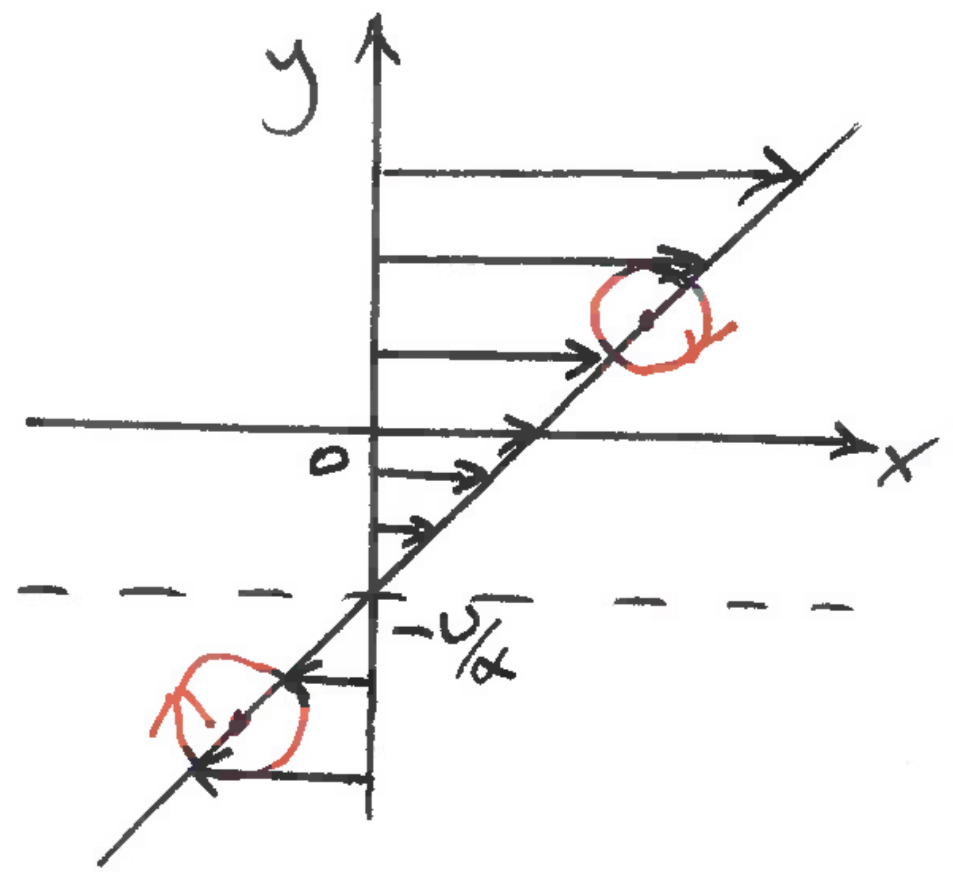
\includegraphics[scale=0.15]{uniformShearFlow.jpeg}
                  	\centering
                    \caption{uniform shear flow illustration}\label{fig:shearFlow}
                \end{figure}
        \end{enumerate}
\end{enumerate}

\subsection{Application --- Double/Repeated Integrals}

Solving double integral involves in the change of variable $(x,y) \rightarrow{}(u,v)$,
transforming the original double integral into:\[
    \iint_{A}^{} f(x,y)\mathrm{d}x\mathrm{d}y = \iint_{A}^{} f(x(u,v),y(u,v))J\mathrm{d}u\mathrm{d}v
\]where $J$ is the \textbf{\emph{Jacobian}} of the transformation.

\begin{figure}
  	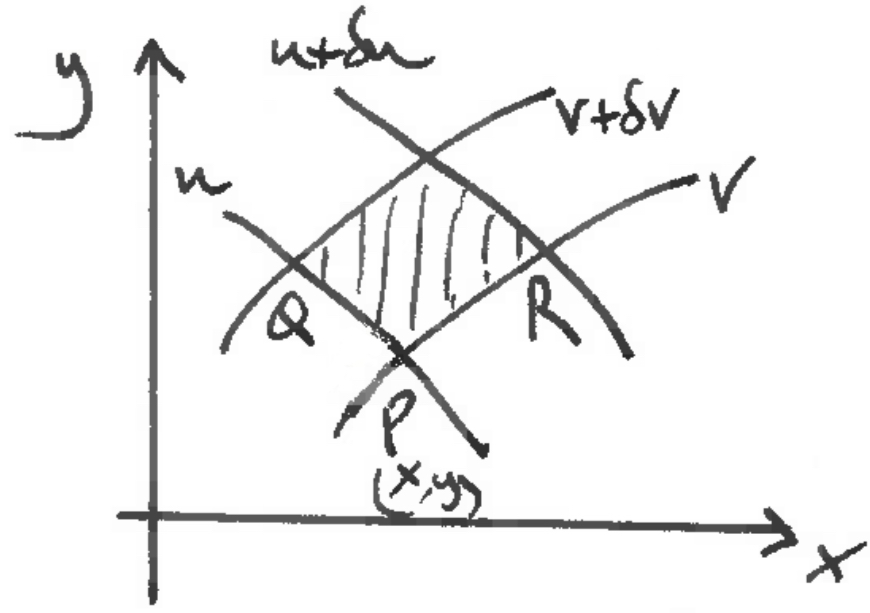
\includegraphics[scale=0.15]{JacobianTransform.jpeg}
  	\centering
    \caption{Jacobian transform illustration}\label{fig:Jacobian}
\end{figure}


One possible illustration is as shown in Figure~\ref{fig:Jacobian}.
The three critical points are $P(x,y), Q\left(x+\frac{\partial x}{\partial v}\delta v, 
y + \frac{\partial y}{\partial v}\delta v\right), 
R\left(x + \frac{\partial x}{\partial u}\delta u, y+\frac{\partial y}{\partial u}\delta u\right)$.
Area of the shaded parallelogram is\[
    \left|\left(\frac{\partial x}{\partial u}\delta u, 
    \frac{\partial y}{\partial u}\delta u\right)
    \times\left(\frac{\partial x}{\partial v}\delta v,
    \frac{\partial y}{\partial v}\delta v\right)\right|
    = J \delta u \delta v
\]where\[
J = \left|\det{\begin{pmatrix}
        \dfrac{\partial x}{\partial u} & \dfrac{\partial x}{\partial v} \\[2ex]
        \dfrac{\partial y}{\partial u} & \dfrac{\partial y}{\partial v}
\end{pmatrix} }\right|
= \nabla x(u,v) \times \nabla y(u,v).
\]

For example, if Cartesian is transformed to polar, i.e.\ $(x,y)\rightarrow{}(r,\theta)$,
since $x=r\cos{\theta}, y=r\sin{\theta}$, then\[
    \frac{\partial x}{\partial r}=\cos{\theta},\;
    \frac{\partial x}{\partial \theta}=-r\sin{\theta},\;
    \frac{\partial y}{\partial r}=\sin{\theta},\;
    \frac{\partial y}{\partial \theta}=r\cos{\theta},
\]\[
\Rightarrow{}J = \left|\det{\begin{pmatrix}
        \cos{\theta} & -r\sin{\theta} \\
        \sin{\theta} & r\cos{\theta}
\end{pmatrix} }\right| = r.
\]


\section{Fourier Integrals}



% End of mathematical methods


\chapter{Linear Algebra}

\section{Introduction to Matrices and Vectors}

\subsection{Column vectors}

\newmdtheoremenv[style=defEnv]{column vector}[theorem]{Definition}
\begin{column vector}
    A \emph{column vector} ($n$-column vector) $\mathbf{v}_n$ is a tuple of $n$ real numbers written as a single columnn, 
    with $a_1, a_2, a_3, \ldots, a_n \in \mathbb{R}$:\[
    \mathbf{v}_n := 
    \begin{pmatrix}
        a_1 \\
        a_2 \\
        a_3 \\
        \vdots \\
        a_n
    \end{pmatrix}
    \]
\end{column vector}

\newmdtheoremenv[style=defEnv]{set of column vectors}[theorem]{Definition}
\begin{set of column vectors}
    $\mathbb{R}^{n}$ is the set of all column vectors of height $n$ whose entries are real numbers.
    In symbols:\[
        \mathbb{R}^{n} = \{
            \begin{pmatrix}
                    a_1\\
                    a_2\\
                    \vdots\\
                    a_n
            \end{pmatrix}
            : a_1, a_2, \ldots, a_n \in \mathbb{R}
        \} 
    \]
\end{set of column vectors}

\begin{ex}
    $\mathbb{R}^{2}$ can be seen as Euclidean plane. $\mathbb{R}^{3}$ can be seen as Euclidean space.
    \\\underline{Caution}: Our vectors always ``start'' at the origin.
\end{ex}

\newmdtheoremenv[style=defEnv]{zero vector}[theorem]{Definition}
\begin{zero vector}
    The \textbf{\emph{zero vector $\mathbf{0}_n$}} is the height $n$-column vector all of whose entries are 0.
\end{zero vector}


\newmdtheoremenv[style=defEnv]{standard basis vector}[theorem]{Definition}
\begin{standard basis vector}
    The \textbf{\emph{standard basis vectors}} in $\mathbb{R}^{n}$ are the vectors\[
        \mathbf{e}_1 = \begin{pmatrix}
                1\\
                0\\
                \vdots\\
                0
        \end{pmatrix}, \quad
        \mathbf{e}_2 = \begin{pmatrix}
                0\\
                1\\
                \vdots\\
                0
        \end{pmatrix}, \quad \ldots, \quad
        \mathbf{e}_n = \begin{pmatrix}
                0\\
                0\\
                \vdots\\
                1
        \end{pmatrix}
    \]
    i.e. $\mathbf{e}_k$ is the vector with $k$th entry equal to 1 and all other entries equal to 0.
\end{standard basis vector}

\paragraph{Operations on column vectors}

    \[
        \mathbf{v} := \begin{pmatrix}
                v_1\\
                v_2\\
                \vdots\\
                v_n
        \end{pmatrix}, \quad
        \mathbf{u} := \begin{pmatrix}
                u_1\\
                u_2\\
                \vdots\\
                u_n
            \end{pmatrix}
    \]
    be column vectors $\mathbb{R}^{n}$, and let $\lambda$ be a (real or complex) number.
    \begin{enumerate}[label = (\arabic*)]
        \item Addition on vectors in $\mathbb{R}^{n}$ is given by:\[
                \begin{pmatrix}
                        v_1 + u_1\\
                        v_2 + u_2\\
                        \vdots\\
                        v_n + u_n
                \end{pmatrix}
            \]$+ : \mathbb{R}^{n} \times \mathbb{R}^{n} \rightarrow \mathbb{R}^{n}$ (binary operatioin).
            $(\mathbb{R}^{n}, +)$ is a group.
        \item \textbf{\emph{Scalar multiplication}} $\lambda \mathbf{v}$ on $\mathbb{R}^{n}$:\[
            \begin{pmatrix}
                    \lambda v_1\\
                    \lambda v_2\\
                    \vdots\\
                    \lambda v_n
            \end{pmatrix}
        \]$s : \mathbb{R} \times \mathbb{R}^{n} \rightarrow \mathbb{R}^{n}$, so not binary operation.
    \item \textbf{\emph{Dot product}} $v \cdot u$ is defined to be the number $v_1 u_1 + v_2 u_2 + \cdots + v_n u_n$.
            $\cdot : \mathbb{R}^{n} \times \mathbb{R}^{n} \rightarrow \mathbb{R}$, so not binary.
    \end{enumerate}

\begin{ex}
    Show that $(\mathbb{R}^{n}, +)$ is an Abelian group.
    \begin{itemize}
        \item Identity: $\mathbf{0}_n$ ($v + \mathbf{0}_n = \mathbf{v}$)
        \item $-\mathbf{v}$ are inverses, where \[
            -\mathbf{v} := \begin{pmatrix}
                    -v_1\\
                    -v_2\\
                    \vdots\\
                    -v_n
            \end{pmatrix}
        \]
        \item associativity: $(\mathbf{u} + \mathbf{v}) + \mathbf{w} = \mathbf{u} + (\mathbf{v} + \mathbf{w})$.
        \item commutative: $\mathbf{u} + \mathbf{v} = \mathbf{v} + \mathbf{u}$
    \end{itemize}
    \underline{Caution}: $+$ only makes sense for vectors of the \emph{same size}.
    e.g. $\mathbf{v} \cdot \mathbf{0}_n = 0 \in \mathbb{R}$.
\end{ex}

\newmdtheoremenv[style=defEnv]{combination of add and scalar multi}[theorem]{Definition}
\begin{combination of add and scalar multi}
    let $\mathbf{v}_1, \mathbf{v}_2, \mathbf{v}_3, \ldots, \mathbf{v}_n \in \mathbb{R}^{n}, \lambda_1, \lambda_2, \lambda_3, \ldots, \lambda_n \in \mathbb{R}$,
    then \[
        \lambda_1 \mathbf{v}_1 + \lambda_2 \mathbf{v}_2 + \cdots + \lambda_n \mathbf{v}_n
    \]is called a \textbf{\emph{linear combination}} of $\mathbf{v}_1, \mathbf{v}_2, \mathbf{v}_3, \ldots, \mathbf{v}_n$.
\end{combination of add and scalar multi}

\newmdtheoremenv[style=defEnv]{span of vectors}[theorem]{Definition}
\begin{span of vectors}
    The set of all linear combinatioins of a collection of vectors $\mathbf{v}_1, \mathbf{v}_2, \ldots, \mathbf{v}_n$
    is called the \textbf{\emph{span}} of the vectors $\mathbf{v}_1, \mathbf{v}_2, \ldots, \mathbf{v}_n$.
    \\Notation: 
    
    span$\left\{\mathbf{v}_1, \mathbf{v}_2,\ldots,\mathbf{v}_n\right\} := 
    \left\{\lambda_1 \mathbf{v}_1 + \lambda_2 \mathbf{v}_2 + \cdots + \lambda_n \mathbf{v}_n 
    | \lambda_1, \ldots, \lambda_n \in \mathbb{R}\right\}$
\end{span of vectors}

\begin{ex}
    compute the span of 
    \begin{itemize}
        \item $\{\mathbf{e}_1, \mathbf{e}_2\}$, $\mathbf{e}_1, \mathbf{e}_2 \in \mathbb{R}^2$.
            \[
                \textnormal{span}\{\mathbf{e}_1, \mathbf{e}_2\} 
                = \{\lambda_1 \mathbf{e}_1 + \lambda_2 \mathbf{e}_2 | \lambda_1, \lambda_2 \in \mathbb{R}\}
            = \{
                    \begin{pmatrix}
                            \lambda_1\\
                            \lambda_2
                    \end{pmatrix}
| \lambda_1, \lambda_2 \in\mathbb{R}\}\]

\item span$\left\{\begin{pmatrix}
        1\\
        0\\
        0
\end{pmatrix}
, \begin{pmatrix}
        0\\
        2\\
        0
\end{pmatrix}
\right\} = \{
\begin{pmatrix}
        \lambda_1\\
        2\lambda_2\\
        0
\end{pmatrix}
| \lambda_1, \lambda_2 \in \mathbb{R}
\}$
    \end{itemize}
    
\end{ex}

\newmdtheoremenv[style=defEnv]{length and norm}[theorem]{Definition}
\begin{length and norm}
    let $\mathbf{v} \in \mathbb{R}^{n}$. The \textbf{\emph{length}} of $\mathbf{v}$, a.k.a.\ the \textbf{\emph{norm}} 
    of $\mathbf{v}$, is the non-negative real number $\lVert\mathbf{v}\rVert$ defined by \[
        \lVert\mathbf{v}\rVert = \sqrt{\mathbf{v} \cdot \mathbf{v}}
    \]
    \underline{Note}: $\lVert\mathbf{0}\rVert = 0$, and conversely if $\mathbf{v} \neq 0$ then $\lVert\mathbf{v}\rVert > 0$.
    This definition agrees with out usual ideas about the length of a vector in $\mathbb{R}^{2}$
    or $\mathbb{R}^{3}$, which follows from Pythagoras' theorem.
\end{length and norm}

\newmdtheoremenv[style=defEnv]{unit vector}[theorem]{Definition}
\begin{unit vector}
    A vector $\mathbf{v} \in \mathbb{R}^{n}$ is called a \textbf{\emph{unit vector}}
    if $\lVert\mathbf{v}\rVert = 1$.
\end{unit vector}

\smallskip
\begin{ex}
    \;

    \begin{enumerate}[label = (\arabic*)]
        \item Any non-zero vector $\mathbf{v}$ can be made into a unit vector
            $\hat{\mathbf{u}} := \frac{\mathbf{v}}{\lVert\mathbf{v}\rVert}$. This process is called \textbf{\emph{normalizing}}.
        \item The standard basis vectors are unit vectors.
    \end{enumerate}
    
\end{ex}

\subsection{Basic Matrix Operations}

\newmdtheoremenv[style=defEnv]{matrix definition}[theorem]{Definition}
\begin{matrix definition}
    An $n \times m$-matrix is a rectangular grid of numbers called the \emph{entries} of the matrix
    with $n$ rows and $m$ columns. A real matrix is onne whose entries are real numbers,
    and a complex matrix is one whose entries are complex numbers.

    \underline{Notations}: $M_{n \times m}(\mathbb{R}), M_{n,m}(\mathbb{R}), \mbox{Mat}_{n\times m}(\mathbb{R}), \mathbb{R}^{n\times m}$.

\end{matrix definition}

\underline{Operations on matrices}:
\newmdtheoremenv[style=defEnv]{matrices operation}[theorem]{Definition}
\begin{matrices operation}
    let $A = (a_{ij})$ and $B = (b_{ij})$ are $n\times m$-matrix, $\lambda \in \mathbb{R}$. Then:
    \begin{enumerate}[label = (\arabic*)]
        \item $A+B = n\times m$-matrix $\,(a_{ij} + b_{ij})$.
            $+: M_{n \times m}(\mathbb{R}) \times M_{n \times m}(\mathbb{R}) \rightarrow M_{n \times m}(\mathbb{R})$
        \item $\lambda A = n \times m$-matrix $\,(\lambda a_{ij})$
    \end{enumerate}
    
\end{matrices operation}

\newmdtheoremenv[style=defEnv]{addition on matrix is Abelian}[theorem]{Theorem}
\begin{addition on matrix is Abelian}
    $(M_{n \times m}(\mathbb{R}), +)$ is an Abelian grouop.
\end{addition on matrix is Abelian}

\newmdtheoremenv[style=defEnv]{transpose}[theorem]{Definition}
\begin{transpose}
    The \textbf{\emph{transpose}} $A^{T}$ of an $n \times m$-matrix $(a_{ij})$ is 
    the $m \times n$-matrix $(a_{ij})$.
    The \textbf{\emph{leading diagonal}} of a matrix is the $(1, 1), (2, 2), \ldots$ entries.
    So the transpose is obtained by doing a reflection in the leading diagonal.
\end{transpose}

\newmdtheoremenv[style=defEnv]{multiplying matrix with vector}[theorem]{(Multiplying matrices with vectors) Definition}
\begin{multiplying matrix with vector}
    Let $A = (a_{ij})$ be an $n \times m$-matrix, $\mathbf{v} \in \mathbb{R}^{m}$.
    Then $A\mathbf{v}$ is the vector in $\mathbb{R}^{n}$ with $i$-th row entry $\sum_{j=1}^{m} a_{ij}\mathbf{v}_j$
\end{multiplying matrix with vector}

\begin{ex}
    \;

    \begin{itemize}
            \item 
                Prove that for $A \in M_{n \times m}(\mathbb{R}), \mathbf{e}_k \in \mathbb{R}^{m}$,
                $A\mathbf{e}_k = k$-th column of A.
    
                \underline{Proof}: let $A = (a_{ij})$. By definition the $i$-th entry of $A\mathbf{e}_k$ is\[
                    \sum_{j=1}^{m} a_{ij}{(\mathbf{e}_k)}_j = a_{ik}
                \]since $ {(\mathbf{e}_k)}_j = 0$ whenever $j \neq k$, 1 for $j = k$
            \item Let $I_n$ be the identity matrix. Show formally that $I_n \mathbf{\nu} = \mathbf{\nu}$, $\forall \mathbf{\nu} \in \mathbb{R}^{n}$.
            \item $\mathbf{\nu} \cdot \mathbf{v} = \mathbf{\nu}^{T} \mathbf{v}$
            \item let $\mathbf{\nu}_1, \mathbf{\nu}_2, \mathbf{\nu}_3 \in \mathbb{R}^{3}$.
                Write the linear combination $3\mathbf{\nu}_1 - 5\mathbf{\nu}_2 + 7\mathbf{\nu}_3$ as a multiplication of matrix
                $A \in M_{3 \times 3}(\mathbb{R})$ with a vector $\mathbf{x} \in \mathbb{R}^{3}$. Then\[
                    A\mathbf{x} = \begin{pmatrix}
                        \mathbf{\nu}_1 & \mathbf{\nu}_2 & \mathbf{\nu}_3
                    \end{pmatrix} 
                    \begin{pmatrix}
                            x_1 \\
                            x_2 \\
                            x_3
                    \end{pmatrix} 
                    = x_1\mathbf{\nu}_1 + x_2\mathbf{\nu}_2 + x_3\mathbf{\nu}_3
                \]
                with $\mathbf{\nu}_1, \mathbf{\nu}_2, \mathbf{\nu}_3$ written as a column vector to form a matrix
                in the above expression, thus using matrix multiplication to express linear combination of vectors.
    \end{itemize}
    
\end{ex}

\section{Systems of linear equations}

\subsection{Definitions}

\newmdtheoremenv[style=defEnv]{linear equation}[theorem]{Definition}
\begin{linear equation}
    A \textbf{\emph{linear equation}} in the variables $x_1, x_2, \ldots, x_n \in \mathbb{R}$
    is an equation of the form:\[
        \lambda_1 x_1 + \lambda_2 x_2 + \cdots + \lambda_n x_n = c, 
        \,\textnormal{with }\, \lambda_1,\ldots,\lambda_n \subset \,\textnormal{\emph{Fixed} real numbers}
    \]
    \underline{Caution}: In particular, no powers/multiplications/function of one or more variables.
\end{linear equation}

\newmdtheoremenv[style=defEnv]{simultaneous list of linear equations}[theorem]{Definition}
\begin{simultaneous list of linear equations}
    A system of $n$ linear equations is a list of simultaneous linear equations.
    It can be converted to $A\mathbf{x} = \mathbf{b} \in \mathbb{R}^{m}$,with\[
        A = \begin{pmatrix}
            a_{11} & a_{12} & \cdots & a_{1n} \\
            a_{21} & a_{22} & \cdots & a_{2n} \\
            \vdots & \vdots & \ddots & \vdots \\
            a_{m1} & a_{m2} & \cdots & a_{mn}
        \end{pmatrix} 
        \in \mathbb{R}^{m \times n}
    \]
\end{simultaneous list of linear equations}
\underline{Caution}: Thee $m \times n$-matrix $A$ is called coefficient matrix.
The matrix $(A|\mathbf{b})$ where the vector $\mathbf{b}$ is added as a column on the  right
is called \textbf{\emph{augmented matrix}}.

\newmdtheoremenv[style=defEnv]{consistent system}[theorem]{Definition}
\begin{consistent system}
    A system is called \textbf{\emph{consistent}} (resp.\ inconsistent)
    if it has a solution $(s_1, s_2, \ldots, s_m)$ (resp.\ no solution).
\end{consistent system}

\begin{ex}
    \[\left\{
        \begin{align*}
            & x_1 + x_3 - x_4 = 1 \\
            & x_2 - x_4 = 6 \\
            & x_1 + x_2 + 6x_3 - 3x_4 = 0
        \end{align*}
     \right.   
    \]
    Augmented matrix form:\[
        \left(\begin{array}{@{}cccc|c@{}}%chktex 4, chktex 44
                1 & 0 & 1 & -1 & 1 \\
                0 & 1 & 0 & -1 & 6 \\
                1 & 1 & 6 & -3 & 0
        \end{array}\right)
    \]
\end{ex}

\newmdtheoremenv[style=defEnv]{row operation}[theorem]{Definition}
\begin{row operation}
    A \textbf{\emph{row operation}} is one of the following procedures on a $n \times m$-matrix $(a_{ij})$:
    \begin{enumerate}[label = (\arabic*)]
        \item $r_i(\lambda)$: multiply row $i$ by a scalar $\lambda \in \mathbb{R}, \lambda \neq 0$.
        \item $r_{ij}$: swap row $i$ with row $j$.
        \item $r_{ij}(\lambda)$: multiply row $i$ by $\lambda \neq 0$, $\lambda \in \mathbb{R}$ and add it to row $j$.
    \end{enumerate}
\end{row operation}

\begin{ex}
    let $A = \begin{pmatrix}
        1 & 2 \\
        3 & 4
    \end{pmatrix} $, so\[
        r_{12} \Rightarrow \begin{pmatrix}
            3 & 4 \\ 
            1 & 2
        \end{pmatrix} 
    \]\[
    r_2(2) \Rightarrow \begin{pmatrix}
        1 & 2\\
        6 & 8
    \end{pmatrix} 
    \]\[
    r_{12}(2) \Rightarrow \begin{pmatrix}
        1 & 2 \\
        5 & 8
    \end{pmatrix} 
    \]
\end{ex}

\newmdtheoremenv[style=defEnv]{row operation on augmented matrix}[theorem]{Proposition}
\begin{row operation on augmented matrix}
    Let $A\mathbf{x} = \mathbf{b}$ be a system of linear equations in matrix form, $(A|\mathbf{b})$
    the augmented matrix, $(A'|\mathbf{b}')$ the augmented matrix of the system after row operation.
    Show that $x$ is solution of $A\mathbf{x} = \mathbf{b} \iff$ $x$ is solution of $A'\mathbf{x} = \mathbf{b}'$.
\end{row operation on augmented matrix}

\begin{proof}
    row operations of type (1) and (2) $\Rightarrow$ trivial.%chktex 10

    (3) Take equation $i$, multiply it by $\lambda$, add it to equation $j$.
    $\Rightarrow (a_{j1} + \lambda a_{i 1}) x_1 + \cdots + (a_{jm} + \lambda a_{im})x_m = b_j + \lambda b_i$.
\end{proof}
\underline{Caution}: Every row operation is invertible: \[
    {[r_i(\lambda)]}^{-1} = r_i(\frac{1}{\lambda}),\; {[r_{ij}]}^{-1} = r_{ij},\;
    {[r_{ij}(\lambda)]}^{-1} = r_{ij}(-\lambda)
\]

\subsection{Gauss algorithm}
\newmdtheoremenv[style=defEnv]{echelon form}[theorem]{Definition}
\begin{echelon form}
    The left most non-zero entry in a non-zero row is called \textbf{\emph{leading entry}}.
    A matrix is called in \textbf{\emph{echelon form}} if:
    \begin{enumerate}[label = (\arabic*)]
        \item The leading entry in each non-zero row is 1.
        \item The leading 1 of each row is to \emph{the right} of the leading 1 in the row above.
        \item The zero-rows are \emph{below} all other rows.
    \end{enumerate}
\end{echelon form}

\begin{ex}
    \[
        \begin{pmatrix}
            0 & 0 & 0 \\
            1 & 0 & 0 \\
            0 & 1 & 0
        \end{pmatrix}, \begin{pmatrix}
        0 & 1 & 0\\
        1 & 0 & 0\\
        0 & 1 & 2
        \end{pmatrix}, \begin{pmatrix}
        1 & 3 & 2 & 0\\
        0 & 1 & 0 & 0\\
        0 & 0 & 0 & 0
        \end{pmatrix} 
    \]
    Only the last one is in echelon form.
\end{ex}

\newmdtheoremenv[style=defEnv]{reduced echelon form}[theorem]{Definition}
\begin{reduced echelon form}
    A matrix is \textbf{\emph{row reduced echelon form}} if:
    \begin{enumerate}[label = (\arabic*)]
        \item It is in echelon form.
        \item The leading 1 in each row is the \emph{only} non-zero entry in its column.
    \end{enumerate}
\end{reduced echelon form}

\begin{ex}
    \[
        \begin{pmatrix}
            1 & 0 & 0 & 3\\
            0 & 0 & 1 & 0\\
            0 & 0 & 0 & 0
        \end{pmatrix}, \begin{pmatrix}
            1 & \alpha & \beta & 2\\
            0 & 0 & 1 & -2
        \end{pmatrix}.
    \]
    The second one is not, unless $\beta = 0$.
\end{ex}

The point of RRE form is that if we have a system of equations\[
    A\mathbf{x} = \mathbf{b}
\]and $A$ is in RRE form, then we can easily read off the solution (if any).
There are four cases to consider:
\begin{enumerate}[label = (\arabic*)]
    \item Every column of $A$ contains a leading 1, and there are no zeros row.
        In this case the only possibility is that $A = I_n$ is the identity matrix.
        Then the equations are simply\[
            \begin{align*}
                x_1 & = b_1 \\
                x_2 & = b_2 \\
                \vdots \\
                x_n & = b_n 
            \end{align*}
        \]
        and they have a unique solution, the entries of $\mathbf{b}$.

    \item Every column of $A$ contains a leading 1, and there are some zero rows.
        Then $A$ must have more rows than columns, and it must be a matrix of the form\[
            A = 
            \begin{pmatrix}
                  I_n \\
                  \mathbf{0}_{k \times n}
            \end{pmatrix} 
        \]
        i.e.\ it looks like an identity matrix with a block of zeros underneath.
        In this case, the first $n$ equations are\[
            \begin{align*}
                x_1 & = b_1 \\
                x_2 & = b_2 \\
                \vdots \\
                x_n & = b_n
            \end{align*}
        \]
        and the last $k$ equations are\[
            \begin{align*}
                0 & = b_{n + 1} \\
                0 & = b_{n + 2} \\
                \vdots \\
                0 & = b_{n + k}
            \end{align*}
        \]
        Now there are two possibilities:
        \begin{itemize}
                \item If any of the last $k$ entries of $\mathbf{b}$ are non-zero
                    then this system has no solutions, because the last $k$ equations
                    are never satisfied for any $\mathbf{x}$ and the system is inconsistent.

                \item If the last $k$ entries of $\mathbf{b}$ are all zero then the system
                    has a unique solution, given by setting $x_i = b_i$ for each $i \in [1, n]$.
        \end{itemize}
        
    \item Some columns of $A$ do not contain a leading 1, but there are no zero rows, for instance\[
        A = \begin{pmatrix}
            1 & 0 & a_{13} \\
            0 & 1 & a_{23}
        \end{pmatrix} 
        \quad \textnormal{or} \quad
        A = \begin{pmatrix}
            1 & a_{12} & 0 \\
            0 & 0 & 1
        \end{pmatrix}.
    \]
    If the $i$th column of $A$ does not contain a leading 1 then the corresponding variable $x_i$
    is called a \textbf{\emph{free variable}}, or free parameter. These variables can be set to
    any values. Each remaining variable is called a \textbf{\emph{basic variable}} and 
    we have a single equation\[
        x_j + (\ldots) = b_j
    \]
    where the expression in the brackets only contains free parameters.
    This equations determines the value of $x_j$, in terms of the entries in $\mathbf{b}$
    and the values of the free parameters.
    This kind of system always has infinitely many solutions, we say it is \textbf{\emph{underdetermined}}.
\end{enumerate}

\newmdtheoremenv[style=defEnv]{pivot position}[theorem]{Definition}
\begin{pivot position}
    A leading entry in a matrix in RRE form is also called a \textbf{\emph{Pivot position}}.
    A \textbf{\emph{Pivot column}} is a column containing a Pivot position.
\end{pivot position}

\newmdtheoremenv[style=defEnv]{Any matrix can convert to RRE}[theorem]{(Gau$\beta$ algorithm) Proposition}
\begin{Any matrix can convert to RRE}
    Any matrix can be put into RRE form by performing a sequence of row operations.
\end{Any matrix can convert to RRE}

\begin{proof}
    Our proof will consist of the explicit description of the algorithm.
    Let $A$ be an arbitrary matrix.
    Step 1---Step 3 below is called the \textbf{\emph{forward phase}}
    and is used to bring the matrix A into echelon form.
    Step 4 is called the \emph{backwad phase}
    and is used to bring $A$ inito RRE form.

    \underline{Step 1}: Choose your first pivot position,
    which is the first non-zero leading term. Do row operation
    such that the leading term becomes 1.

    \underline{Step 2}: Create zeros below your first leading entry by
    multiplying the row with the leading entry and subtract it from the subsequent rows.

    \underline{Step 3}: Repeat the first two steps to bring the whole matrix into echelon form.

    \underline{Step 4}: Create zeros above the leading entries to convert to RRE row by row,
    by multiplying the row where the selected leading entry is in, and subtract it from the above rows.

\end{proof}

    \medskip
    It is also true (althouth we won't show this) that the RRE form of a matrix is unique;
    if you apply any sequence of row operations which puts your matrix into RRE form,
    the result is the same as the output of the algorithm we just described.

    Now we have a systematic procedure for solving a system of simultaneous linear equations
    $A\mathbf{x} = \mathbf{b}$:
    \begin{enumerate}[label = (\arabic*)]
        \item Form the augmented matrix $(A|\mathbf{b})$.
        \item Apply the algorithm above to put the augmented matrix into RRE form $(A'|\mathbf{b}')$.
        \item Read off the solutions to $A'\mathbf{x} = \mathbf{b}'$
    \end{enumerate}
    
    In fact it's not necessary to get the whole matrix $(A'|\mathbf{b}')$ into RRE form, 
    you can stop when the left block $A'$ is in RRE form. Doing further operations to adjust
    the final column will not help you read the solutions.


\begin{ex}
    Solve\[
        \left\{
            \begin{align*}
                & 3x_1 + 5x_2 - 4x_3 = 0 \\
                & -3x_1 - 2x_2 + 4x_3 = 0 \\
                & 6x_2 + x_2 - 8x_3 = 0. \\
            \end{align*}
            \right.
    \]
    The RRE form of the above equation is\[
        \begin{pmatrix}
            1 & 0 & -\frac{4}{3} & 0 \\
            0 & 1 & 0 & 0 \\
            0 & 0 & 0 & 0
        \end{pmatrix} 
    \]
    and the geometric interpretation of this is a line!
\end{ex}

\newmdtheoremenv[style=defEnv]{Solutions to a system is 0, 1, infinity}[theorem]{Proposition}
\begin{Solutions to a system is 0, 1, infinity}
    The number of solutions to a system $A\mathbf{x} = \mathbf{b}$ is always either 0, 1, or $\infty$.
\end{Solutions to a system is 0, 1, infinity}

\begin{proof}
    Assume the number of solutions is not 0, and not 1.
    Take 2 solution $\nu$ and $\upsilon$, $\mathbf{\nu} \neq \mathbf{\upsilon}$.\[
        \Rightarrow{} A\mathbf{\nu} = A\mathbf{\upsilon} = b \Rightarrow{}
        A(\mathbf{\nu} - \mathbf{\upsilon}) = 0 = \omega \neq 0
    \]
    Take: $\nu + \lambda \omega, \lambda \in \mathbb{R}$\[
        \Rightarrow{} A(\nu + \lambda\omega) = A\nu + \lambda A\omega = A\mathbf{\nu} = \mathbf{b} = \mathbf{b}
    \]
    So $\mathbf{\nu} + \lambda \mathbf{\omega}$ is a solution $\forall \lambda \in \mathbb{R}$
    $\Rightarrow{} \infty$ many solutions.
\end{proof}

\section{Matrix Multiplication}

\subsection{Basics of Matrix Multiplication}

\newmdtheoremenv[style=defEnv]{matrix multiplicatioin}[theorem]{Definition}
\begin{matrix multiplicatioin}
    $A \in M_{m, n}(\mathbb{R}), B \in M_{n, k}(\mathbb{R})$. Then the product $AB$
    is defined such that the ${(AB)}_{ik} = \sum_{j = 1}^{n} a_{ij}b_{jk}$ (row $i$ column $k$)
\end{matrix multiplicatioin}

\underline{Operation}: $M_{m,n}(\mathbb{R}) \times M_{n, k}(\mathbb{R}) \rightarrow{} M_{m, k}(\mathbb{R})$.
It is a binary operation on $M_{n,n}(\mathbb{R})$, square matrices! 
Be careful with the size of the matrices.

\bigskip
\underline{Caution}:

\begin{itemize}
    \item The $(i, j)$-entry of $AB$ is the dot product of $r_i^{T}$ with $c_j$.

    \item Other way to see it: column $j$ of $AB$ is $Ac_j$.
\end{itemize}

\newmdtheoremenv[style=defEnv]{matrix properties}[theorem]{Proposition}
\begin{matrix properties}
    Let $A, A' \in M_{m,n}(\mathbb{R}), B, B' \in M_{n,p}(\mathbb{R})$. Then
    \begin{enumerate}[label = (\arabic*)]
        \item $A(BC) = (AB)C$. (Associativity)
        \item \[
            \left\{
                \begin{align*}
                    & A(B + B') = AB + AB' \\
                    & (A + A')B = AB + A'B
                \end{align*}
            \right\} \quad \textnormal{Distributivity}
        \]
                
    \item $\forall \lambda \in \mathbb{R}, (\lambda A)B = A(\lambda B) = \lambda (AB)$.
        (Compatibility with scalar multiplication.)
    \end{enumerate}
    
\end{matrix properties}


\underline{Caution}: 
\begin{itemize}
    \item Let $A \in M_{m,n}(\mathbb{R})$, then $0_{k \times m} A = 0_{k\times n},
        A 0_{n \times e} = 0_{m \times e}$.

    \item $\forall A \in M_{n,n}(\mathbb{R}), I_n A = AI_n = A$.

    \item In general, $AB \neq BA$, i.e.\ not commutative.

    \item $A^2$ does not guarantee to be $0_{n, n}$, e.g.\ $\begin{pmatrix}
            0 & 0 \\
            1 & 0 
    \end{pmatrix} $
\end{itemize}

\newmdtheoremenv[style=defEnv]{diagonal matrix}[theorem]{Definition}
\begin{diagonal matrix}
    A \textbf{\emph{diagonal matrix}} is a square matrix $D \in M_{n,n}(\mathbb{R})$, s.t.\[
        \left\{
            \begin{align*}
                & D_{ij} = 0, i \neq j \\
                & D_{ij} = \lambda_i \in \mathbb{R}, i = j
            \end{align*}
        \right.
    \]
    Goal: When can we bring matrices to this form? $\leadsto$ diagonalization.
    E.g. $I_n, 0_{n\times n}$.
\end{diagonal matrix}

\newmdtheoremenv[style=defEnv]{upper and lower triangular matrix}[theorem]{Definition}
\begin{upper and lower triangular matrix}
    \textbf{\emph{Lower triangular matrix}}: $a_{ij} = 0, i < j$. (strictly lower if $i \le j$)
    \textbf{\emph{Upper triangular matrix}}: $a_{ij} = 0, i > j$. (strictly upper if $i \ge j$)
\end{upper and lower triangular matrix}

\begin{ex}
    echelon form, RRE (Upper triangular).
    Lower + upper triangular = diagonal.
\end{ex}

\subsection{Inverse of a Matrix and Invertibility}

\newmdtheoremenv[style=defEnv]{inverse square matrix}[theorem]{Definition}
\begin{inverse square matrix}
    Let $A \ini M_{n,n}(\mathbb{R})$. A $n \times n$-matrix $A^{-1}$ is called \textbf{\emph{inverse}}
    of $A$ if:\[
        AA^{-1} = I_n = A^{-1}A.
    \]
    \underline{Caution}: Not all matrices are \emph{invertible}!
\end{inverse square matrix}

\newmdtheoremenv[style=defEnv]{lemma Of inverse matrix}[theorem]{Lemma}
\begin{lemma Of inverse matrix}
    \,

    \begin{enumerate}[label = (\arabic*)]
        \item If $A$ is invertible, then its inverse is unique.
        \item If $A$ is invertible and either $AB = I_n$ or $BA = I_n$, for some $B \ini M_{n\times n}(\mathbb{R})$,
            then $B = A^{-1}$.
    \end{enumerate}
    
\end{lemma Of inverse matrix}

\begin{proof}
    \,

    \begin{enumerate}[label = (\arabic*)]
        \item See group theory.
        \item $B = I_n B = (A^{-1} A)B = A^{-1} (AB) = A^{-1} I_n = A^{-1}$.
            Same for $BA$.
    \end{enumerate}
    
\end{proof}

\newmdtheoremenv[style=defEnv]{AB = A-1 B-1}[theorem]{Lemma}
\begin{AB = A-1 B-1}
    Assume $A,B \in M_{n \times n}(\mathbb{R})$, invertible.
    Then $AB$ is invertible and ${(AB)}^{-1} = B^{-1}A^{-1}$.
\end{AB = A-1 B-1}

\newmdtheoremenv[style=defEnv]{invertibility}[theorem]{Lemma}
\begin{invertibility}
    Let $A \in M_{n \times n}(\mathbb{R})$.
    \begin{enumerate}[label = (\arabic*)]
        \item If $\exists \mathbf{\upsilon} \in \mathbb{R}^{n}, \mathbf{\upsilon} \neq \mathbf{0}$ 
            s.t. $A\mathbf{\upsilon} = \mathbf{0}$, then $A$ is not invertible.

            (extended: same if $\mathbf{\upsilon} \in \mathbb{R}^{n}^{T}, \mathbf{\upsilon}A = \mathbf{0}$.)
        \item If $\exists B \in M_{n \times n}(\mathbb{R}), B \neq 0_{n \times n}$ s.t.
            $AB = 0_{n \times n}$ or $BA = 0_{n \times n}$, then $A$ is not invertible.
    \end{enumerate}
\end{invertibility}

\begin{proof}
    \,

    \begin{enumerate}[label = (\arabic*)]
        \item (contrapositive) Assume $A$ is invertible $\iff \exists A^{-1} \in M_{n\times n}(\mathbb{R})$,
            s.t. $AA^{-1} = A^{-1}A = I_n$.
            Assume $A\mathbf{\upsilon} = 0$, so 
            $A^{-1}A\upsilon = I_n \upsilon = \upsilon$, contradiction.
        \item Assume $BA = 0_{n\times n}$. $A$ invertible $\Rightarrow{}\exists A^{-1}$
            s.t. $AA^{-1} = I_n$.
            Therefore $B = BI_{n} = B(AA^{-1}) = (BA)A^{-1} = 0_{n\times n}$, contradiction.
    \end{enumerate}
\end{proof}

\newmdtheoremenv[style=defEnv]{invertible so row/column of zero}[theorem]{Corollary}
\begin{invertible so row/column of zero}
    If $A \in M_{n\times n}(\mathbb{R})$ invertible, then it cannot have a row/column of zeros.
\end{invertible so row/column of zero}

\begin{proof}
    Exercise!
\end{proof}

\newmdtheoremenv[style=defEnv]{elementary matrix}[theorem]{Definition}
\begin{elementary matrix}
    An \textbf{\emph{elementary matrix}} $R$ is a matrix which differs from $I_n \in M_{n \times n}(\mathbb{R})$
    by only \emph{one} elementary row operation.
    Multiplying a matrix by the elementary matrix on the left is equivalent of performing an
    elementary row operation on that matrix.
\end{elementary matrix}

\begin{description}
    \item[Type 1] Apply $r_i(\lambda)$ to $I_n$.
        Multiplying $A \in M_{n\times n}(\mathbb{R})$ by $R_i(\lambda)$
        on the left.
        
    \item[Type 2] Apply $r_{ij}$ to $I_n$.
        Multiplying $A$ by $R_{ij}$ on the left swaps row $i$ and $j$ in $A$.

    \item[Type 3] Apply $r_{ij}(\lambda)$ to $I_n$.
\end{description}

\underline{Fact}: Elementary matrices are \emph{invertible} since row operations are reversible.
You can always produce an inverse of an elementary matrix which represents the reversed
process of elementary row operation.

\newmdtheoremenv[style=defEnv]{elementary row operations are invertible}[theorem]{Lemma}
\begin{elementary row operations are invertible}
    Let $A \in M_{n\times n}(\mathbb{R})$, $A'$ obtained from $A$
    by elementary row operations.
    Then $A$ invertible $\iff$ $A'$ invertible.
\end{elementary row operations are invertible}

\begin{proof}
    $A \in M_{n\times n}(\mathbb{R})$. Say we got $A'$ from $A$ by row operation.
    $A' = RA$ for some $R$ elementary matrix, Both $A$ and $R$ are invertible.
    Then $A'$ is invertible, and $A'^{-1} = A^{-1}R^{-1}$.

    For `$\Leftarrow$', $A' = RA \iff R^{-1}A' = A$.
\end{proof}

\newmdtheoremenv[style=defEnv]{invertible A'}[theorem]{Lemma}
\begin{invertible A'}
    $A\in M_{n\times n}(\mathbb{R})$, $A'$ the RRE form of $A$. Then:
    $A'$ invertible $\iff$ $A'$ has no zero rows.
\end{invertible A'}

\begin{proof}
    ``$\Leftarrow$'': Assume $A'$ has no zero rows $\Rightarrow{}$ A' has a leading one in each column.
    $\Rightarrow{}A' = I_n$.
\end{proof}

\newmdtheoremenv[style=defEnv]{invertible matrix is identity itself}[theorem]{Corollary}
\begin{invertible matrix is identity itself}
    $A$ is invertible $\iff$ Its RRE form is the identity matrix.
\end{invertible matrix is identity itself}

\underline{Algorithm to compute inverse}:

\begin{description}
    \item[Step 1] Write the augmented matrix $(A|I_n)$.
    \item[Step 2] Bring $(A|I_n)$ to RRE form
        $\rightarrow{}(A|I_n)\rightarrow{}(R_1A|R_1 I_n)\rightarrow{}\cdots
        \rightarrow{}(R_m\cdots R_2 R_1 A|R_m\cdots R_2 R_1)$.
    \item[Step 3] Read result.
\end{description}

\begin{ex}
    \[
        A = \begin{pmatrix}
            0 & 1 & 2 \\
            1 & 0 & 3 \\
            4 & -3 & 8
        \end{pmatrix} 
    \]and calculate its inverse!

    \[
            \begin{align*}
                (A|I_3) & = \begin{pmatrix}
                    0 & 1 & 2 & 1 & 0 & 0 \\
                    1 & 0 & 3 & 0 & 1 & 0 \\
                    4 & -3 & 8 & 0 & 0 & 1
                \end{pmatrix} \\
                        & = \begin{pmatrix}
                            1 & 0 & 3 & 0 & 1 & 0 \\
                            0 & 1 & 2 & 1 & 0 & 0 \\
                            4 & -3 & 8 & 0 & 0 & 1
                        \end{pmatrix} \\
                        & = \begin{pmatrix}
                            1 & 0 & 3 & 0 & 1 & 0 \\
                            0 & 1 & 2 & 1 & 0 & 0 \\
                            0 & -3 & -4 & 0 & -4 & 1
                        \end{pmatrix} \\
                        & = \begin{pmatrix}
                            1 & 0 & 3 & 0 & 1 & 0 \\
                            0 & 1 & 2 & 1 & 0 & 0 \\
                            0 & 0 & 2 & 3 & -4 & 1
                        \end{pmatrix} \\
                        & = \begin{pmatrix}
                            1 & 0 & 3 & 0 & 1 & 0 \\
                            0 & 1 & 2 & 1 & 0 & 0 \\
                            0 & 0 & 1 & \frac{3}{2} & -2 & \frac{1}{2}
                        \end{pmatrix} \\
                        & \vdots \\
                        & = \begin{pmatrix}
                            1 & 0 & 0 & -\frac{9}{2} & 7 & -\frac{3}{2} \\
                            0 & 1 & 0 & -2 & 4 & -1 \\
                            0 & 0 & 1 & \frac{3}{2} & -2 & \frac{1}{2}
                        \end{pmatrix} 
            \end{align*}
        \]
\end{ex}

\underline{Caution}: If at any point you get a row of 0s, Stop! (matrix not invertible)
\underline{Caution}: Now that we know how to get inverses. Consider:
$A\mathbf{x} = \mathbf{b}$. (system of linear equations)
If $A$ invertible: $A^{-1}\mathbf{b} = \mathbf{x}$. (Solution is unique.)

\subsection{Determinant}

\newmdtheoremenv[style=defEnv]{determinant}[theorem]{Definition}
\begin{determinant}
    let $A = \begin{pmatrix}
        a_{11} & a_{12} \\
        a_{21} & a_{22}
    \end{pmatrix} $,
    so det $A = a_{11}a_{22} - a_{21}a_{12}\neq 0 \iff A$ is invertible.
\end{determinant}

\newmdtheoremenv[style=defEnv]{submatrix}[theorem]{Definition}
\begin{submatrix}
    Let $A \in M_{n\times n} (\mathbb{R})$. $A_{ij}$ is the \textbf{\emph{submatrix}} obtained
    by deleting row $i$ and column $j$ of $A$. $A_{ij}$ is called the $(i,j)$-minor.
\end{submatrix}

\newmdtheoremenv[style=defEnv]{determinant of nxn matrix}[theorem]{Definition}
\begin{determinant of nxn matrix}
    The \textbf{\emph{determinant}} of an $n\times n$-matrix $A = (a_{ij})$ is given by:\[
        \det{A} = \sum_{j}^{} {(-1)}^{j + i} a_{ij} \det{A_{ij}}
        = \sum_{i}^{} {(-1)}^{i + j} a_{ij} \det{A_{ij}}.
    \]
    The first expression is called the \emph{expansion along the $i$-th row},
    while the second expression is called the \emph{expansion along the $j$-th column}.
\end{determinant of nxn matrix}

\begin{ex}
    Find the determinant of\[
        \begin{pmatrix}
            1 & 0 & 1 & 0 \\
            0 & 1 & 0 & 1 \\
            2 & 2 & 1 & 0 \\
            0 & 0 & 2 & 1
        \end{pmatrix}.
    \]
\end{ex}

\paragraph{Rules for determinants}
Let $A \in M_{n\times n}(\mathbb{R})$.
\begin{enumerate}[label = (\arabic*)]
    \item Operation $r_i(\lambda)$ produces matrix $B$, s.t. $\det{B} = \lambda \det{A}$.
    \item Operation $r_{ij}$ produces matrix $B$, s.t. $\det{B} = - \det{A}$.
    \item Operation $r_{ij}(\lambda)$ leaves determinant invariant.
    \item let $B \in M_{n\times n}(\mathbb{R})$, $\det{AB} = \det{A} \cdot \det{B}$.
    \item $\det{A} = \det{A^{T}}$.
\end{enumerate}

\newmdtheoremenv[style=defEnv]{invertible matrix is not 0}[theorem]{Proposition}
\begin{invertible matrix is not 0}
    $n\times n$-matrix $A$ is invertible $\iff \det{A} \neq 0$.
\end{invertible matrix is not 0}

\begin{proof}
    \,

    \begin{itemize}
            \item ``$\Rightarrow{}$'': Assume $A$ invertible
                $\Rightarrow{} \exists A^{-1}$ s.t. $AA^{-1} = I_n$.
                ($\det{I_n} = 1$!) So
                $\det{(AA^{-1})} = \det{A}\cdot\det{A^{-1}} = \det{I_n} = 1$.
                Therefore $\det{A} \neq 0 \neq \det{A^{-1}}$.

            \item ``$\Leftarrow$'': Assume $\det{A} \neq 0$.
                Since elementary matrices are invertible, their determinants are $\neq 0$,
                so the determinant of RRE form $A'$ is going to be $\neq 0$
                $\Rightarrow{}A' = I_n \Rightarrow{}A$ invertible.
    \end{itemize}
\end{proof}

\newmdtheoremenv[style=defEnv]{permutation theory}[theorem]{Definition}
\begin{permutation theory}
    Let $\sigma \in S_n$. An \textbf{\emph{inversion}} is a pair of integers $(i,j)$ s.t.:\[
        0 < i < j \le n \quad\textnormal{and}\quad \sigma(i)\ge\sigma(j).
    \]
    The \textbf{\emph{sign}} of a permutation $\textnormal{sgn}\;\sigma$ is given by
    \begin{itemize}
            \item $+1$, if number of inversion is even
            \item $-1$, if number of inversion is odd.
    \end{itemize}
\end{permutation theory}

\newmdtheoremenv[style=defEnv]{det of A}[theorem]{Definition}
\begin{det of A}
    Let $A \in M_{n,n}(\mathbb{R})$, then \[\det{A} = 
    \sum_{\sigma \in S_n}^{} \textnormal{sgn}\,\sigma\, a_{1\sigma(1)}a_{2\sigma(2)}\cdots a_{n\sigma(n)}.\]
\end{det of A}

\begin{ex}
        Let $A = I_n$. Show that $\det{I_n} = 1$.
\end{ex}

\section{Eigenvalues and Eigenvectors}

\subsection{Basic Definitions}

\newmdtheoremenv[style=defEnv]{eigenvalue and vector}[theorem]{Definition}
\begin{eigenvalue and vector}
    Let $A \in M_{n\times n}(\mathbb{R}), \lambda \in \mathbb{R}, \lambda$ is an \textbf{\emph{eigenvalue}}
    to the \textbf{\emph{eigenvector}} $\mathbf{\mathbf{v}} \in \mathbb{R}^{n}\backslash\{\mathbf{0}\}$ if\[
        A\mathbf{\mathbf{v}} = \lambda\mathbf{\mathbf{v}}.
    \]
    Geometrically, applying $A$ to $\mathbf{\mathbf{v}}$ just ``rescales'' $\mathbf{\mathbf{v}}$.
\end{eigenvalue and vector}

\underline{Warning}:
\begin{itemize}
    \item $\mathbf{\mathbf{v}}$ eigenvector $\iff (A-\lambda I_n)\mathbf{\mathbf{v}} = \mathbf{0}$.
    \item $I_n \mathbf{\mathbf{v}} = \mathbf{\mathbf{v}} \,\forall \mathbf{\mathbf{v}} \neq \mathbf{0}$
        $\Rightarrow{}$ 1 is the only eigenvalue to \emph{all} vectors.
    \item $0_{n\times n} \mathbf{\mathbf{v}} = \mathbf{0}_n = 0\cdot\mathbf{\mathbf{v}}$ 
        $\Rightarrow{}$ 0 is the only eigenvalue to \emph{all} vectors.
\end{itemize}

\newmdtheoremenv[style=defEnv]{eigenvalue property}[theorem]{Proposition}
\begin{eigenvalue property}
    Let $A \in M_{n\times n}(\mathbb{R})$.
    Then $\lambda$ is eigenvalue of $A$ $\iff$ $A-\lambda I_n$ is not invertible.
\end{eigenvalue property}

\begin{proof}
    $A$ invertible $\iff$ $\exists n$ non-zero vectors s.t. $A\mathbf{\upsilon} = \mathbf{0}$.
    Since we want \emph{non-zero} solutions of $(A - \lambda I_n)\mathbf{\upsilon} = 0$,
    $A - \lambda I_n$ cannot be invertible!
\end{proof}

\begin{ex}
    $A = \begin{pmatrix}
        1 & 2\\
        2 & 1
    \end{pmatrix}$. Find the eigenvalues.

    Augmented matrix:\[
        \begin{pmatrix}
            1 - \lambda & 2 & 0 \\
            2 & 1 - \lambda & 0
        \end{pmatrix}.
    \]
    \begin{description}
        \item[Case 1] $\lambda = 1 \Rightarrow{}$ RRE is $I_2$, not what we want!
        \item[Case 2] Assume $\lambda \neq 1$. Convert to RRE,
            and to ensure that the matrix is not invertible,
            $\lambda^{2} - 2\lambda - 3 = 0 \Rightarrow{} \lambda = -1, 3$.
    \end{description}
\end{ex}

\newmdtheoremenv[style=defEnv]{trace of A}[theorem]{Definition}
\begin{trace of A}
    \textbf{\emph{Trace}} of $A_{n\times n}(\mathbb{R})$ tr $A$ is $\sum_{i=1}^{n} a_{ii}$.
\end{trace of A}

\newmdtheoremenv[style=defEnv]{characteristic polynomial}[theorem]{Definition}
\begin{characteristic polynomial}
    The \textbf{\emph{characteristic polynomial}} of $A_{2\times 2}(\mathbb{R})$ is\[
        \lambda^{2} - \textnormal{tr}\,A\;\lambda + \det{A}.
    \]In general, for $A_{n\times n}(\mathbb{R})$ is\[
    \det{(A - \lambda I_n)}.
    \]
\end{characteristic polynomial}

\subsection{Diagonalization}

\newmdtheoremenv[style=defEnv]{diagonalization}[theorem]{Definition}
\begin{diagonalization}
    Let $A,B \in M_{n\times n}(\mathbb{R})$. $A$ and $B$ are called \textbf{\emph{similar}} if
    $\exists P \in M_{n\times n}(\mathbb{R})$ invertible s.t.\[
        A = P^{-1}BP.
    \]
    $A$ is called \textbf{\emph{diagonalizable}} if $B$ is diagonal.
    If $A$ is similar to $B$, then $B$ is similar to $A$.
\end{diagonalization}

\newmdtheoremenv[style=defEnv]{similar matrices have the same eigenvalues}[theorem]{Proposition}
\begin{similar matrices have the same eigenvalues}
    Similar matrices have the same eigenvalues.
\end{similar matrices have the same eigenvalues}

\begin{proof}
    To solve: \[
        \begin{align*}
            0 & = \det{(A-\lambda I_n)} \\
              & = \det{(P^{-1}BP - \lambda I_n)} \\
              & = \det{(P^{-1}BP - \lambda P^{-1}P)} \\
              & = \det{(P^{-1}(B-\lambda I_n)P)} \\
              & = \det{P^{-1}} \det{(B-\lambda I_n)} \det{P} \\
              & = \det{(P^{-1}P)}\det{(B-\lambda I_n)} \\
              & = 1 \cdot \det{(B-\lambda I_n)} \\
              & = \det{(B-\lambda I_n)}.
        \end{align*}
    \]
\end{proof}

\underline{Warning}: The eigenvectors are in general \emph{not} the same.
But if $A\mathbf{\upsilon} = \lambda \mathbf{\upsilon} \iff P^{-1}BP\mathbf{\upsilon} = \lambda\mathbf{\upsilon}$
$\iff B(P\mathbf{\upsilon}) = \lambda (P\mathbf{\upsilon})$.

\newmdtheoremenv[style=defEnv]{eigenvalues of D}[theorem]{Lemma}
\begin{eigenvalues of D}
    Let $A \in M_{n\times n}(\mathbb{R})$. Assume $\mathbf{\upsilon}_1, \mathbf{\upsilon}_2,\ldots,\mathbf{\upsilon}_n$
    are eigenvectors of $A$. Then if $P = (\mathbf{\upsilon}_1 \quad \mathbf{\upsilon}_2 \,\cdots\, \mathbf{\upsilon}_n)$
    is invertible, then $A$ is diagonalizable and $A = PDP^{-1}$ with $D$'s leading
    diagonal entries being the eigenvalues $\lambda_1, \lambda_2, \ldots, \lambda_n$.
\end{eigenvalues of D}

\begin{proof}
    We can consider $P^{-1}AP = D \iff AP = PD$.
    Look at the $k$-th column vector of $AP$: $A\mathbf{\upsilon}_k = \lambda_k \mathbf{\upsilon}_k$.
    Look at the $k$-th column vector of $PD$: $P\lambda_k e_k$, which 
    the diagonal identity matrix ``extracts'' out the eigenvectors one by one.
    ($e_k$ is an identity matrix)
\end{proof}

\section{Vector Space}

\subsection{Axioms and Examples}

\newmdtheoremenv[style=defEnv]{vector space}[theorem]{Definition}
\begin{vector space}
    A \textbf{\emph{vector space}} is a set $V$ together with
                \begin{itemize}
                        \item a binary operation: $+:V\times V \rightarrow{} V$,
                            $(v, \nu) \mapsto v + \nu$.
                        \item a scalar multiplication: $\mathbb{R}\times V \rightarrow{} V$,
                            $(\lambda, \nu) \mapsto \lambda \nu$.
                \end{itemize}
              such that:
              \begin{enumerate}[label = (\arabic*)]
                  \item $(V,+)$ is an Abelian group
                  \item $1 \cdot \nu = \nu$.
                  \item $\forall \lambda, \mu \in \mathbb{R}, \nu \in V$:
                      $\lambda(\mu\nu) = (\lambda\mu)\nu$
                  \item $\forall \lambda \in \mathbb{R}, \nu,v \in V$:
                      $\lambda(v +\nu) = \lambda v + \lambda\nu$
                  \item $\forall \lambda, \mu \in \mathbb{R}, \nu \in V$,
                      $(\lambda + \mu)\nu = \lambda\nu + \mu\nu$.
              \end{enumerate}
              There are 9 axioms to be satisfied!
\end{vector space}

\begin{ex}
    \,

    \begin{enumerate}[label = (\arabic*)]
        \item Our ``model'': $\mathbb{R}^{n}$. Especially $\mathbb{R}$ is a vector space.

        \item 
            $\mathbb{R}{[x]}_{\le n} = \left\{a_0+ a_1x + a_2x^{2} + \cdots + a_n x^{n}
            |a_0, a_1,\ldots, a_n\in \mathbb{R}, x\in \mathbb{R}\right\} $.

        \item $M_{n,m}(\mathbb{R})$.
    \end{enumerate}
    
\end{ex}

\newmdtheoremenv[style=defEnv]{vector space property}[theorem]{Lemma}
\begin{vector space property}
    $V$ is vector space, $x \in V$, then
    \begin{enumerate}[label = (\arabic*)]
        \item $\forall n \in \mathbb{N}, nx = x + x + \cdots + x$.
        \item $0 x = 0_V$.
        \item $(-1)x$ is additive inverse.
    \end{enumerate}
\end{vector space property}

\begin{proof}
    \,

    \begin{enumerate}[label = (\arabic*)]
        \item $1v = v \forall v \in V$.
            $2v = (1 + 1)v = 1v + 1v = v + v$.
            Induction!

        \item $0x = (0 + 0)x = 0x + 0x$.
            Since there is an inverse of $0x$ because addition is Abelian,
            add it on both sides:\[
                0_V = 0x + {(0x)}^{-1} = 0x + 0x + {(0x)}^{-1} = 0x + 0_V = 0x.
            \]

        \item $0_V = 0x = (1 + (-1))x = 1x + (-1)x = x + (-1)x$, therefore
            $(-1)x = x^{-1}$ over addition.
    \end{enumerate}
\end{proof}

\newmdtheoremenv[style=defEnv]{subspace}[theorem]{Definition}
\begin{subspace}
    Let $V$ be a vector space. A subset $U \subseteq V$ is called \textbf{\emph{subspace}} if:
    \begin{enumerate}[label = (\arabic*)]
        \item If $x, y \in U$, $x + y \in U$. (Closure on addition)
        \item If $x \in U, \lambda \in \mathbb{R}$, then $\lambda x \in U$. (Closure on scalar multiplication)
        \item $0_V \in U$. (equivalent to saying $U \neq \varnothing$)
    \end{enumerate}
\end{subspace}

\underline{Note}: $(U, +)$ is an Abelian group.

\begin{ex}
    \,

    \begin{enumerate}[label = (\arabic*)]
        \item Let $U \in \mathbb{R}^{3}, U = \{\begin{pmatrix}
                x \\
                y \\
                z
        \end{pmatrix} | x + y + z = 0\}$.
        It is geometrically a plane! (spanned by $\begin{pmatrix}
                -1 \\
                1 \\
                0
        \end{pmatrix}$ and $\begin{pmatrix}
                -1 \\
                0 \\
                1
            \end{pmatrix}$.) It ``looks'' like $\mathbb{R}^{2}$.

        \item Let $U \subseteq \mathbb{R}^{\mathbb{R}} 
            := \left\{F | F:\mathbb{R} \mapsto \mathbb{R}\right\}$,
            $U := \left\{F | F(\pi) = 0\right\} $.
            (Be careful with the $e$, treat it as $0^{f}:x\mapsto 0$)

        \item $U := \left\{\lambda v | \lambda \in \mathbb{R}\right\} \subseteq V $.

        \item Every vector space has two \emph{trivial} subspaces: itself and $\{0_V\}$.
    \end{enumerate}

    If $U \subseteq V$ is a subspace which is neither itself nor $\{0_V\}$, then
    it is called a \textbf{\emph{proper}} subspace.
\end{ex}

\newmdtheoremenv[style=defEnv]{union and intersection of subspaces}[theorem]{Lemma}
\begin{union and intersection of subspaces}
    Let $V$ be a vector space, $U, W \subseteq V$ are subspaces, then
    \begin{enumerate}[label = (\arabic*)]
        \item $U \cap W$ is a subspace.
        \item $U \cup W$ is \emph{not} a subspace.
            (Unless $U \subseteq W$ and $W \subseteq U$.)
    \end{enumerate}
\end{union and intersection of subspaces}

\begin{proof}
    Exercise! (Write it out rigorously!)
\end{proof}

\paragraph{Remark}
\begin{itemize}
        \item 
    Concrete example for (2): let $U = \{\begin{pmatrix}
            x \\
            0
    \end{pmatrix} | x \in \mathbb{R}\}, W = \{\begin{pmatrix}
            0 \\
            y
    \end{pmatrix} | y \in \mathbb{R}\}$. Both subspaces form a coordinate system,
    and their addition forms the coordinates on the coordinate system!

    \item $U + V := \{x + y | x \in U, y \in W\}$ is a subspace of $V$. (Exercise)
\end{itemize}

\subsection{Spanning Sets}

\newmdtheoremenv[style=defEnv]{spanning sets}[theorem]{Definition}
\begin{spanning sets}
    Let $V$ be a vector space, $S \subseteq V$ be a subset.
    A \textbf{\emph{linear combination}} of elements $v_1, v_2, \ldots, v_n \in S$ is a vector $x \in V$:\[
        x = \lambda_1 v_1 + \lambda_2 v_2 + \cdots + \lambda_n v_n
    \]where $\lambda_1, \lambda_2, \ldots, \lambda_n \in \mathbb{R}$.
\end{spanning sets}

Subsequently, all $V$ denotes a vector space.

\newmdtheoremenv[style=defEnv]{subspace and linear combination}[theorem]{Lemma}
\begin{subspace and linear combination}
    Let $U \neq \varnothing, U \subseteq V$, then $U$ is a subspace $\iff$
    every linear combination of element of $U$ is in $U$.
\end{subspace and linear combination}

\begin{proof}
    Exercise!
\end{proof}

\newmdtheoremenv[style=defEnv]{span of a subset of vector space}[theorem]{Definition}
\begin{span of a subset of vector space}
    Let $S \subseteq V$ be a subset $S \neq \varnothing$,\[
        \textnormal{Span}\,S:= \{\lambda_1 v_1 + \lambda_2 v_2 + \cdots + \lambda_n v_n |
        \lambda_1, \lambda_2, \ldots, \lambda_n \in \mathbb{R}, v_1, v_2, \ldots, v_n \in S\}.
    \]
    In addition, \[
        \textnormal{Span}\,\varnothing := \{0_V\}.
    \]
\end{span of a subset of vector space}

\newmdtheoremenv[style=defEnv]{span S is a subspace}[theorem]{Proposition}
\begin{span S is a subspace}
    Span $S$ is a subspace of $V$.
\end{span S is a subspace}

\begin{proof}
    Exercise!
\end{proof}

\newmdtheoremenv[style=defEnv]{spanning set S}[theorem]{Definition}
\begin{spanning set S}
    Set $S$ is called the \textbf{\emph{spanning set}} if Span $S = V$.
\end{spanning set S}

\begin{ex}
    Take Span$\{e_1, e_2, e_3\}$ $= \mathbb{R}^{3}$,
    which forms the normal 3-D coordinate system we usually see.
    So $\left\{e_1, e_2, e_3\right\}$ is the spanning set of $\mathbb{R}^{3}$.
\end{ex}

\newmdtheoremenv[style=defEnv]{span of subset of subspace}[theorem]{Lemma}
\begin{span of subset of subspace}\label{lemma:1}
    $S \subseteq V$ subset, $S \subseteq U$ for some subspace $U \subseteq V$.
    Then span $S \subseteq U$.
\end{span of subset of subspace}

\emph{\underline{Notation}}: Subsequently, $\subset$ and $\subseteq$ are used interchangeably,
``strictly a subset of'' is represented by $\subsetneq$,
denoting ``a proper subset'', and depening on additional conditions,
``a proper subspace''.

\begin{proof}
    $U$ subspace $\Rightarrow{}$ closed under addition + scalar multiplication
    $\Rightarrow{}$ closed under taking linear combination.
    Then since $S \subseteq U \Rightarrow{}$ Span $S \subseteq U$ by definition.
\end{proof}

\underline{Warning}: If $S$ is a spanning set of $V$, it cannot be contained 
in any proper subspace of $V$.
(If $S \subseteq U$ for some subspace $U \subset V$, 
then $U$ is \emph{not} closed under linear combinations of elements of $S$.)

\newmdtheoremenv[style=defEnv]{finite spanning set}[theorem]{Definition}
\begin{finite spanning set}
    A vector space is called \textbf{\emph{finite-dimensional}} if it has a \emph{finite spanning set}.
\end{finite spanning set}

\underline{Notation}: $\dim{V} < \infty$.

\underline{Note}: If you want to prove that a vector space $V$ is \emph{not} finite-dimensional
then it is not enough to find an infinite spanning set: you have to prove that no finite spanning set exists.
Indeed, every vector space (except the zero vector space) has an infinite spanning set, 
e.g.\ the set $S = V$.

\newmdtheoremenv[style=defEnv]{dimension def}[theorem]{Definition}
\begin{dimension def}
    The \textbf{\emph{dimension}} of a finite-dimensional vector space,
    written as $\dim{V}$,
    is the size of the smallest spanning set.
\end{dimension def}

\begin{ex}
    \begin{itemize}
        \,

            \item 
    Consider the vector space ${\mathbb{R}[X]}_{\le d}$ of all polynomials of degree at most $d$.
    This is finite-dimensional, since the subset $S = \left\{1, X, X^{2},\ldots,X^{d}\right\} $
    is a spanning set.
\item Consider the vector space $\mathbb{R}[X]$. It is not finite-dimensional.
    Suppose we pick a finite set $S = \left\{P_1,P_2,\ldots,P_n\right\} \subset \mathbb{R}[X]$.
    Each polynomial $P_i$ has some degree $d_i$, and if we set $d = \max{(d_1, d_2,\ldots,d_n)}$,
    then $S$ is contained in the proper subspace ${\left\{\mathbb{R}[X]\right\}}_{\le d}$.
    So by the previous lemma, the subset $S$ is not a spanning set.
    \end{itemize}
    
\end{ex}

\subsection{Linear independence}

\newmdtheoremenv[style=defEnv]{linear independence}[theorem]{Definition}
\begin{linear independence}
    A subset $L \subset V$ is called \textbf{\emph{linearly dependent}} if
    we can find \emph{distinct} vectors $\mathbf{v}_1, \mathbf{v}_2,\ldots,\mathbf{v}_n \in L$
    and \emph{non-zero} scalars $\lambda_1 \neq 0, \lambda_2 \neq 0,\ldots,\lambda_n \neq 0$ s.t.\[
        \lambda_1 \mathbf{v}_1 + \lambda_2 \mathbf{v}_2 + \cdots + \lambda_n \mathbf{v}_n = \mathbf{0}_V.
    \]
    If $L$ is not linearly dependent we say that it is \textbf{\emph{linearly independent}}.
\end{linear independence}

\underline{Note}: If $L' \subset L$ and $L'$ is linearly-dependent,
then $L$ is also linearly-dependent (just use the same $\mathbf{v}_i$'s and $\lambda_i$'s).
So if $L$ is linearly-independent then any subset of $L$ is also linearly-independent.

\begin{ex}
    If $\mathbf{0}_V \in L$ then $L$ is linearly-dependent,
    because we can take any $\lambda \neq 0$ and observe that $\lambda \mathbf{0}_V = \mathbf{0}_V$.
\end{ex}

\newmdtheoremenv[style=defEnv]{basis}[theorem]{Definition}
\begin{basis}
    A \textbf{\emph{basis}} of a vector space is a linearly independent spanning set.
    The plural of basis is \textbf{\emph{bases}}.
\end{basis}

\newmdtheoremenv[style=defEnv]{v can be written with element of basis}[theorem]{Proposition}
\begin{v can be written with element of basis}\label{prop:1}
    Let $B = \left\{\mathbf{v}_1, \mathbf{v}_2, \ldots, \mathbf{v}_n\right\} \subset V$ be a (finite)
    basis of vector space $V$. Then every vector in $V$ can be written as a linear combination
    of elements in $B$, in a \emph{unique} way.
    Conversely, any finite subset $B$ with the above property is a basis.
\end{v can be written with element of basis}

\begin{proof}
    Exercise!
\end{proof}

\newmdtheoremenv[style=defEnv]{coefficients of x with respect to B}[theorem]{Definition}
\begin{coefficients of x with respect to B}
    If we find a (finite) basis $B = \left\{\mathbf{v}_1,\ldots,\mathbf{v}_n\right\} $,
    then any vector $\mathbf{x} \in V$ can be uniquely expressed as\[
        \mathbf{x} = \lambda_1 \mathbf{v}_1 + \cdots + \lambda_n \mathbf{v}_n.
    \]The scalars $\lambda_i$ are called the \textbf{\emph{coefficients of $x$ with respect to $B$}}.
    Every vector $\mathbf{x}\in V$ corresponds to a unique set of coefficients
    $\lambda_1, \lambda_2, \ldots, \lambda_n$.
\end{coefficients of x with respect to B}
To put it more formally, the basis $B$ allows us to define a function\[
    \begin{align*}
        F_B:\mathbb{R}^{n} & \mapsto V \\
        \begin{pmatrix}
                \lambda_1 \\
                \lambda_2 \\
                \vdots \\
                \lambda_n
            \end{pmatrix} & \mapsto \lambda_1 \mathbf{v}_1 + \cdots + \lambda_n \mathbf{v}_n.
    \end{align*}
\]
What Proposition~\ref{prop:1} says is that the function $F_B$ is a bijection.
Note that $F_B^{-1}$ sends a vector $\mathbf{x}$ to its coefficients with respect to $B$.

\newmdtheoremenv[style=defEnv]{linearly dependent spanning set removed an element to be linearly independent}[theorem]{Lemma}
\begin{linearly dependent spanning set removed an element to be linearly independent}
    Let $S \subset V$ be a spanning set, and suppose that $S$ is not linearly independent.
    Then $\exists \mathbf{x}\in S$ s.t. $S' = S\backslash\left\{\mathbf{x}\right\} $ is still a spanning set.
\end{linearly dependent spanning set removed an element to be linearly independent}

\begin{proof}
    Exercise!
    (Be careful that after removing an element from the spanning set,
    you need to show that it is not a spanning set of a subspace!)
    
    Set $S' = S \backslash\left\{\mathbf{s}_1\right\} $. Then $\mathbf{s}_1 \in \;\textnormal{span}\;{S'}$,
    and trivially $S' \subset \;\textnormal{span}\;{S'}$, so $S \subset \;\textnormal{span}\;{S'}$.
    By Lemma~\ref{lemma:1}, span $S \subset$ span $S' \Rightarrow{} V \subset$ span $S'$.
    This implies that span $S' = V$.
\end{proof}

\newmdtheoremenv[style=defEnv]{any finite spanning set contains a basis}[theorem]{Corollary}
\begin{any finite spanning set contains a basis}
    Any finite spanning set contains a basis.
\end{any finite spanning set contains a basis}

\begin{proof}
    Exercise!
\end{proof}

\newmdtheoremenv[style=defEnv]{any finite-dimensional v has a basis}[theorem]{Corollary}
\begin{any finite-dimensional v has a basis}
Any finite-dimensional vector space $V$ has a basis.
\end{any finite-dimensional v has a basis}

\begin{proof}
    Exercise!
\end{proof}

\newmdtheoremenv[style=defEnv]{Steinitz exchange lemma}[theorem]{Proposition}
\begin{Steinitz exchange lemma}
Let $S \subset V$ be a spanning set of $V$, and let $L = \left\{\mathbf{x}_1, \ldots, \mathbf{x}_n\right\} $
be a \emph{finite linearly independent} subset of $V$, then 
$\exists T = \left\{\mathbf{y}_1,\ldots,\mathbf{y}_n\right\} \subset S$, with the same size as $L$, s.t.\[
    S' = (S\backslash T)\cup L
\]is a spanning set.
\end{Steinitz exchange lemma}

\begin{proof}
    Exercise!
\end{proof}

\newmdtheoremenv[style=defEnv]{finite spanning set and linearly independent set}[theorem]{Corollary}
\begin{finite spanning set and linearly independent set}
    Let $V$ be a finite-dimensional vector space, $S \subset V$ be a finite spanning set
    and $L \subset V$ be a linearly independent subset.
    Then $L$ is finite and $|L| \le |S|$.
\end{finite spanning set and linearly independent set}

\newmdtheoremenv[style=defEnv]{dimension and basis}[theorem]{Theorem}
\begin{dimension and basis}
    Let $V$ be a finite-dimensional vector space with $\dim{V} = n$.
    Then any basis of $V$ is finite and has size $n$.
\end{dimension and basis}

\begin{proof}
    Exercise! (Hint: use $\le, \ge$ to deduce $=$.)
\end{proof}

Therefore, to check dimension,
we just need to check if the spanning set is a basis and count its elements.

\subsection{Dimension of Subspaces}

\newmdtheoremenv[style=defEnv]{linearly independent subset of V}[theorem]{Lemma}
\begin{linearly independent subset of V}
    Assume $L \subseteq V$ linearly independent, $v \in V$, $v \notin \span{L}$,
    then $L \cup \{v\}$ still linearly independent.
\end{linearly independent subset of V}

\begin{proof}
    Exercise!
\end{proof}

\newmdtheoremenv[style=defEnv]{infinite dimension find basis subset}[theorem]{Lemma}
\begin{infinite dimension find basis subset}
    If $V$ is \emph{not} finite dimensional ($\dim{V} = \infty$),
    then $\forall n\in \mathbb{N}, \exists L \subset V$ 
    linearly independent subset s.t. $|L| = n$.
\end{infinite dimension find basis subset}

\begin{proof}
    Exercise! (Hint: Induction!) Write it out formally!
\end{proof}

\newmdtheoremenv[style=defEnv]{linearly independent subset of size n}[theorem]{Lemma}
\begin{linearly independent subset of size n}
    Let $\dim{V} < \infty = n$. Then any linearly independent subset of size $n$ is a basis.
\end{linearly independent subset of size n}

\begin{proof}
    Exercise! (Use contradiction!)
\end{proof}

\newmdtheoremenv[style=defEnv]{linearly independent subset is contained in basis}[theorem]{Lemma}
\begin{linearly independent subset is contained in basis}
    Let $\dim{V} < \infty$, then any linearly independent subset is contained in a basis.
\end{linearly independent subset is contained in basis}

\begin{proof}
     Exercise!
\end{proof}

You can prove by adding linearly independent elements to the set, and
this procedure is called \textbf{\emph{basis extension}}.

\begin{ex}
    \[
    v_1 = \begin{pmatrix}
            0 \\
            1 \\
            0
    \end{pmatrix} , v_2 = \begin{pmatrix}
            -2 \\
            0 \\
            1
    \end{pmatrix} \in \mathbb{R}^{3}
\]are linearly independent. Extend it to a basis.

\[
    \span{\{\begin{pmatrix}
            0 \\
            1 \\
            0
    \end{pmatrix} ,\begin{pmatrix}
            -2 \\
            0 \\
            1
\end{pmatrix} \}} = \{\begin{pmatrix}
        x \\
        y \\
        z
\end{pmatrix} | x + 2z = 0\} \subset \mathbb{R}^{3}.
\]
So for instance, $v = \begin{pmatrix}
        1 \\
        0 \\
        0
    \end{pmatrix} \notin \span{L}$.
\end{ex}

\newmdtheoremenv[style=defEnv]{finite dimension subspace}[theorem]{Proposition}
\begin{finite dimension subspace}
    Let $\dim{V} = n < \infty$, $U \subseteq V$ subspace. Then
    \begin{enumerate}[label = (\arabic*)]
        \item $U$ is finite dimension
        \item $\dim{U} \le \dim{V}$
        \item $\dim{U} = \dim{V} \Rightarrow{} U=V$.
    \end{enumerate}
    
\end{finite dimension subspace}

\begin{proof}
    Exercise!
\end{proof}


\begin{ex}
    Possible subspaces of $\mathbb{R}^{2}$. (dim 0, 1, 2)
    ($\dim{\mathbb{R}^{2}}$)
    If $n = 0: \{0_V\}$ (0 vector space, \emph{not} $\varnothing$!)
    If $n = 2: \mathbb{R}^{2}$.

    Proper subspaces have dimension $n = 1$ iff it has a one-dimensional \emph{basis} $\{v\} = L$.
    $\span{L} = \{\lambda v | \lambda \in \mathbb{R}\}$, which is a line passing through the origin.
\end{ex}

\section{Linear Maps}

\subsection{Definitions and Properties}

\newmdtheoremenv[style=defEnv]{linear map}[theorem]{Definition}
\begin{linear map}
    Let $U,V$ be vector spaces. A function $f:U\mapsto V$ is called \textbf{\emph{linear}} if:
    \begin{enumerate}[label = (\arabic*)]
        \item $f(u+v) = f(u) + f(v)$
        \item $f(\lambda v) = \lambda f(v)$
    \end{enumerate}
    where $u, v \in U$.
\end{linear map}

\begin{ex}
    \,

    \begin{enumerate}[label = (\arabic*)]
        \item Let $A \in M_{n,k}(\mathbb{R}), T_A: \mathbb{R}^{k} \rightarrow{} \mathbb{R}^{n}$,
            $x \mapsto Ax$.
        \item $0 : U \rightarrow{} V$, $u \mapsto 0_V$.
        \item $V = \mathbb{R}[x]$ (vector space of all polynomials).
            $D: \mathbb{R}[x] \rightarrow{} \mathbb{R}[x]$,
            $P \mapsto \frac{\mathrm{d}P}{\mathrm{d}x} (= P') =: D(P)$.
        \item $f:\mathbb{R}^{2}\rightarrow{}\mathbb{R}$,
            $\begin{pmatrix}
                    x \\
                    y
            \end{pmatrix} \mapsto x^{2}+ y^{2}$.
    \end{enumerate}
\end{ex}

\newmdtheoremenv[style=defEnv]{0v linear map}[theorem]{Lemma}
\begin{0v linear map}
    $f:U\rightarrow{}V$ is linear $\Rightarrow{} f(0_U) = 0_V$.
\end{0v linear map}

\begin{proof}
    $f(0_U) = f(0_U + 0_U) = f(0_U) + f(0_U)$.
    Then by taking the inverse of $f(0_U)$ on both sides,
    i.e.\ minus $f(0_U)$ on both sides, because only addition is defined,
    so $f(0_U) = 0_V$.
\end{proof}

\underline{Warning}: The converse is not true!

\newmdtheoremenv[style=defEnv]{composite function is linear}[theorem]{Lemma}
\begin{composite function is linear}
    Let $f:U\rightarrow{}V, g:V\rightarrow{}W$ be linear,
    then $g\circ f : U\rightarrow{}W$ is also linear.
\end{composite function is linear}

\begin{proof}
    Exercise!
\end{proof}

\newmdtheoremenv[style=defEnv]{image of function}[theorem]{Definition}
\begin{image of function}
    Let $f:U\rightarrow{}V$ be linear.
    Then the \textbf{\emph{image}} of $f$ is: Im $f:= \{f(u) | u \in U \} \subseteq V$.
    The \textbf{\emph{kernel}} of $f$ is: Ker $f:=\{u \in U | f(u) = 0_V\} \subseteq U$.
\end{image of function}

\newmdtheoremenv[style=defEnv]{ker and im are subspaces}[theorem]{Lemma}
\begin{ker and im are subspaces}
    Let $f:U\rightarrow{}V$ be linear. 
    Then ker $f\subseteq U$ and Im $f\subseteq V$ are subspaces.
\end{ker and im are subspaces}

\begin{proof}
    Exercise!
\end{proof}

\begin{ex}
    $A \in M_{1,3}(\mathbb{R}), A = (1, 1, 1)$.
    $T_A:\mathbb{R}^{3} \rightarrow{} \mathbb{R}, x \mapsto Ax$
    s.t.\[
        \begin{pmatrix}
                x \\
                y \\
                z
        \end{pmatrix} \mapsto A \begin{pmatrix}
                x \\
                y \\
                z
        \end{pmatrix} = x + y + z.
    \]
    ker $T_A := \{v \in \mathbb{R}^{3} | T_A v = 0_\mathbb{R}\} =
        \{\begin{pmatrix}
                x \\
                y \\
                z
        \end{pmatrix} \in \mathbb{R}^{3} | x + y + z = 0\}$.
\end{ex}

\newmdtheoremenv[style=defEnv]{injective linear map iif ker = 0V}[theorem]{Lemma}
\begin{injective linear map iif ker = 0V}
    A linear map $f:U\rightarrow{}V$ is injective $\iff$ ker $f = \{0_U\}$.
\end{injective linear map iif ker = 0V}

\begin{proof}
    Exercise!
\end{proof}

\newmdtheoremenv[style=defEnv]{preimage}[theorem]{Definition}
\begin{preimage}
    The \textbf{\emph{preimage}} of $y$ is the set
    $f^{-1}(y) = \{x\in U | f(x) = y\}$.
\end{preimage}

\newmdtheoremenv[style=defEnv]{preimage = x + elements of kernel}[theorem]{Lemma}
\begin{preimage = x + elements of kernel}
    Let $f:U\rightarrow{} V$ linearly, $y \in V$ fixed.
    Suppose $x \in U$ s.t. $f(x) = y$. Then\[
        f^{-1}(y) = \{x + v | v \in \ker{f}\}.
    \]
\end{preimage = x + elements of kernel}

\begin{proof}
    Exercise! (Warning: it is very hard to prove directly that two sets are equal!
    Instead, use $\subseteq$ and $\supseteq$ to derive $=$)
    Be careful with what you are proving, is it $=$ or $\subseteq$?
    For set, if proving $=$ directly, ensure that it is \emph{bi-directional}.
\end{proof}

\begin{ex}
    $A \in M_{n,k}(\mathbb{R})$, $b \in \mathbb{R}^{n}$.
    $A\mathbf{x} = b, \mathbf{x} \in \mathbb{R}^{k} \iff T_A \mathbf{x} = b$.
    There are three possibilities:
    \begin{enumerate}[label = (\arabic*)]
        \item No solution: $b \notin $ Im $T_A$.
        \item one solution: $b \in$ Im $T_A$, $\ker{T_A} = \{0_{\mathbb{R}^{k}}\}$.
        \item $\infty$-many solution $b \in$ Im $T_A$, $\dim{\ker{T_A}} \neq 0$.
    \end{enumerate}
\end{ex}

\newmdtheoremenv[style=defEnv]{linear map has a matrix representation}[theorem]{Definition}
\begin{linear map has a matrix representation}
    Let $f:\mathbb{R}^{k} \rightarrow{} \mathbb{R}^{n}$ be linear.
    Then $f \equiv T_A$ for some matrix $A \in M_{n,k}(\mathbb{R})$.
\end{linear map has a matrix representation}

\begin{proof}
   Exercise! (It is constructive proof!)
\end{proof}

\newmdtheoremenv[style=defEnv]{same basis tranformed implies same linear map}[theorem]{Proposition}
\begin{same basis tranformed implies same linear map}
    Let $f:U\rightarrow{}V, g:U\rightarrow{}V$ be linear.
    $B = \{b_1, b_2,\ldots,b_k\}$ basis of $U$.
    Assume $f(b_i) = g(b_i) \;\forall i$, then $f = g$.
\end{same basis tranformed implies same linear map}

\newmdtheoremenv[style=defEnv]{sdfsdf}[theorem]{Proposition}
\begin{sdfsdf}
    Let $U,V$ vector spaces, $B = \{b_1, b_2,\ldots,b_k\}$ basis of $U$,
    $\{v_1, v_2,\ldots,v_k\} \subset V$.
    Then there exists a \emph{unique linear} map s.t. $f(b_i) = v_i \;\forall i$.
\end{sdfsdf}

\begin{proof}
    Exercise! (There are three things to prove! $f(b_i) = v_i$, linear, and unique!)
\end{proof}

\subsection{Isomorphism}

\newmdtheoremenv[style=defEnv]{isomorphism}[theorem]{Definition}
\begin{isomorphism}
    A linear map $f:U\rightarrow{}V$ between two vector spaces is called an \textbf{\emph{isomorphism}}
    if $f$ is bijective.
    If there exists an isomorphism from $U$ to $V$,
    we say that $U$ is \textbf{\emph{isomorphic}} to $V$, and write\[
        U \cong V.
    \]
\end{isomorphism}

\underline{Note}: $f^{-1}$ is also an isomorphism, i.e.\ $U \cong V \iff V \cong U$.
Since $f$ is bijective, it is surjective $\Rightarrow{}$ Im $f = V$,
and injective $\Rightarrow{} \ker{f} = \{\mathbf{0}_U\}$.

\begin{ex}
    $\mathbb{R}{[X]}_{\le d} \cong \mathbb{R}^{d+1}, M_{2, 2}(\mathbb{R}) \cong \mathbb{R}^{4}$.
\end{ex}

\newmdtheoremenv[style=defEnv]{isomorphic to Rn}[theorem]{Proposition}
\begin{isomorphic to Rn}
    Let $V$ be a vector space with $\dim{V} = n$.
    Then $V$ is isomorphic to $\mathbb{R}^{n}$.
\end{isomorphic to Rn}

\begin{proof}
    Exercise! (Remember to prove that the linear map is bijective!)
\end{proof}

\newmdtheoremenv[style=defEnv]{C is basis iif f is isomorphism}[theorem]{Lemma}
\begin{C is basis iif f is isomorphism}
    Let $f:U\rightarrow{}V$ be a linear map, $B=\{\mathbf{b}_1, \mathbf{b}_2,\ldots,\mathbf{b}_k\}$
    be a basis for $U$. Let $C = \{f(\mathbf{b}_1),\ldots,f(\mathbf{b}_k)\} \subset V$, then:
    \begin{enumerate}[label = (\roman*)]
        \item $C$ is a spanning set iff $f$ is surjective
        \item $C$ is linearly independent iff $f$ is injective
        \item $C$ is a basis iff $f$ is an isomorphism.
    \end{enumerate}
\end{C is basis iif f is isomorphism}

\begin{proof}
    Exercise!
\end{proof}

\newmdtheoremenv[style=defEnv]{isomorphic vector spaces have the same dimension}[theorem]{Corollary}
\begin{isomorphic vector spaces have the same dimension}
    If $U \cong V$ then $\dim{U} = \dim{V}$.
\end{isomorphic vector spaces have the same dimension}

\begin{proof}
    Exercise!
\end{proof}

\newmdtheoremenv[style=defEnv]{linear map over two V of same dim}[theorem]{Corollary}
\begin{linear map over two V of same dim}
    Let $f:U\rightarrow{}V$ be a linear map, $\dim{U} = \dim{V}$, then the following are equivalent:
    \begin{enumerate}[label = (\roman*)]
        \item $f$ is injective
        \item $f$ is surjective
        \item $f$ is an isomorphism.
    \end{enumerate}
\end{linear map over two V of same dim}

\begin{proof}
    Exercise!
\end{proof}

\newmdtheoremenv[style=defEnv]{find basis in new vector space}[theorem]{Corollary}
\begin{find basis in new vector space}
    If $f:\mathbb{R}^{n}\rightarrow{}V$ is an isomorphism, then the set\[
        C = \{f(\mathbf{e}_1), f(\mathbf{e}_2),\ldots, f(\mathbf{e}_n)\}
    \]is a basis of $V$.
\end{find basis in new vector space}

\subsection{Rank-Nullity theorem}

\newmdtheoremenv[style=defEnv]{def of rank and nullity}[theorem]{Definition}
\begin{def of rank and nullity}
    Let $U$ and $V$ be vector spaces, $f:U\rightarrow{}V$ be a linear map, then:
    \begin{itemize}
        \item the \textbf{\emph{rank}} of $f$, written as rank $f$,
            is the dimension of Im $f$, i.e.\ $\dim{\textnormal{Im}\; f}$
        \item the \textbf{\emph{nullity}} of $f$, written as null $f$,
            is the dimension of $\ker{f}$, i.e.\ $\dim{\ker{f}}$.
    \end{itemize}
\end{def of rank and nullity}

\newmdtheoremenv[style=defEnv]{rank-nullity theorem}[theorem]{Theorem}
\begin{rank-nullity theorem}
    Let $U$ and $V$ be vector spaces, $f:U\rightarrow{}V$ be a linear map, then\[
        \;\textnormal{rank}\;f + \;\textnormal{null}\;f = \dim{U}.
    \]
\end{rank-nullity theorem}

\begin{proof}
    Exercise!
\end{proof}

\begin{ex}
    \,

    \begin{enumerate}[label = (\alph*)]
        \item 
            \[
                \begin{align*}
                    D:\mathbb{R}{[X]}_{\le n} & \rightarrow{}\mathbb{R}{[X]}_{\le n - 1} \\
                    P & \mapsto \frac{\mathrm{d}P}{\mathrm{d}X}.
                \end{align*}
            \]
            The kernel of $D$ is the subspace\[
                \ker{D} = \mathbb{R}{[X]}_{\le 0} \subset \mathbb{R}{[X]}_{\le n}
            \]which has dimension 1. The image of $D$ is the subspace\[
                \;\textnormal{Im}\;D = \mathbb{R}{[X]}_{\le n - 1}
            \]which has a dimension $n$. And indeed $\mathbb{R}{[X]}_{\le n}$ has dimension $n + 1$.

        \item Let $T_A:\mathbb{R}^{3}\rightarrow{}\mathbb{R}^{3}$,
            $v\mapsto Av$, with $A = \begin{pmatrix}
                1 & 2 & 0 \\
                0 & 0 & 1 \\
                0 & 0 & 0
            \end{pmatrix}$. Then\[
            \ker{T_A} = \{v|Av = 0_{\mathbb{R}^{3}}\} = \;\textnormal{span}\;\{\begin{pmatrix}
                    1 \\
                    -\frac{1}{2} \\
                    0
            \end{pmatrix}\}.
            \]Hence the nullity of $T_A$ is 1, and its rank is 2, since $\mathbb{R}^{3}$ has dimension 3.

        \item Let $A \in M_{n\times k}(\mathbb{R})$ be a matrix in RRE form, and
            $T_A:\mathbb{R}^{k} \rightarrow{} \mathbb{R}^{n}$ the associated linear map.
            Suppose that $r$ of the columns of $A$ containing a leading 1.
            Then from the definition of RRE form it's clear that Im $T_A$ contains
            the first $r$ standard basis vectors $\mathbf{e}_1, \ldots, \mathbf{e}_r \in \mathbb{R}^{n}$,
            and that these vectors span Im $T_A$, so the rank of $T_A$ is $r$.
            Then the Rank-Nullity theorem says that\[
                \;\textnormal{null}\;T_A = \dim{\{\mathbf{u}\in \mathbb{R}^{k}, A\mathbf{u} = \mathbf{0}\}} = k - r.
            \]This is the same as the number of `free parameters' for this system of linear equations.
    \end{enumerate}
    
\end{ex}





% End of Linear Algebra




\chapter{Analysis}

\section{Sequence and Convergence}

\newmdtheoremenv[style=defEnv]{sequence}[theorem]{Definition}
\begin{sequence}
    A \textbf{\emph{sequence}} (of real numbers) is a map (function) $F: \mathbb{N} \mapsto \mathbb{R}$.
\end{sequence}

\newmdtheoremenv[style=defEnv]{triangle inequality}[theorem]{(Triangle Inequality) Theorem}
\begin{triangle inequality}
    Triangle inequality: $|x-y| \le |x-z| + |z-y|$. (most common form: $|x+y| \le |x| + |y|$)

    ``Reversed'' triangle inequality: $||x|-|y|| \le |x-y|$.
\end{triangle inequality}

\begin{proof}
    Assume $|x| \ge |y|$, and replace $x$ with $x - y$ in $||x|-|y|| \le |x-y|$:\[
        |x| \le |x-y|+|y| \Rightarrow{}||x|-|y|| \le |x|-|y| \le |x-y|.
    \]
\end{proof}

\newmdtheoremenv[style=defEnv]{convergent sequences}[theorem]{Definition}
\begin{convergent sequences}
    A sequence $a_n$ is \textbf{\emph{convergent}} if \[
        \exists L \in \mathbb{R} \;\textnormal{s.t.}\; \forall \epsilon > 0,
        \exists N \in \mathbb{N} \;\textnormal{s.t.}\; \forall n \ge N, |a_n - L| \le \epsilon.
    \]
\end{convergent sequences}

\newmdtheoremenv[style=defEnv]{divergent sequences}[theorem]{Definition}
\begin{divergent sequences}
    A sequence $a_n$ is called \textbf{\emph{divergent}} if\[
        \forall L \in \mathbb{R}, \exists \epsilon > 0 \;\textnormal{s.t.}\;
        \forall N \in \mathbb{N}, \exists n \ge N \;\textnormal{s.t.}\; |a_n - L| \ge \epsilon.
    \]
\end{divergent sequences}

\begin{ex}
    \,

    \begin{enumerate}[label = (\arabic*)]
        \item $a_n = \frac{1}{n} \rightarrow{} 0$.
            (Hint: Use Archimedian property: $\forall \epsilon > 0, \exists N \in \mathbb{N}$
            s.t. $N > \frac{1}{\epsilon}$.)
            
        \item $a_n = C \rightarrow{} C$.

        \item $a_n = n$ is divergent.

        \item $a_n = {(-1)}^{n}$ is divergent.
            (Hint: applying triangle inequality, $|a_n - a_{n + 1}| = 
            |a_n - L + L - a_{n + 1}| \le |a_n - L| + |L - a_{n - 1}|$.)
    \end{enumerate}
    
\end{ex}

\newmdtheoremenv[style=defEnv]{shift of (an)}[theorem]{Definition}
\begin{shift of (an)}
    Let $(a_n)$ be a sequence, $S \in \mathbb{N}$.
    The \textbf{\emph{shift}} of $(a_n)$ by $S$ is the sequence $b_n := a_{n+S}$.
\end{shift of (an)}

\newmdtheoremenv[style=defEnv]{shift of (an) converges if (an) converges}[theorem]{Lemma}
\begin{shift of (an) converges if (an) converges}
    Let $(a_n)$ be a sequence, $S \in \mathbb{N}$, and $b_n := a_{n + S}$, then
    $b_n$ converges $\iff$ $a_n$ converges.
\end{shift of (an) converges if (an) converges}

\begin{proof}
    Exercise!
\end{proof}

\newmdtheoremenv[style=defEnv]{increasing and decreasing sequence}[theorem]{Definition}
\begin{increasing and decreasing sequence}
    A sequence is (strictly) decreasing if $\forall n\in \mathbb{N}, a_{n + 1}\le a_n$ (resp. $a_{n + 1} < a_n$).
    A sequence is (strictly) increasing if $\forall n \in \mathbb{N}, a_{n + 1}\ge a_n$ (resp. $a_{n + 1} > a_n$).
\end{increasing and decreasing sequence}


\newmdtheoremenv[style=defEnv]{bounded def}[theorem]{Definition}
\begin{bounded def}
    Let $(a_n)$ be a sequence. Then:
    \begin{itemize}
        \item $(a_n)$ is \textbf{\emph{bounded above}} if $\exists R_1 \in \mathbb{R}$ s.t. $a_n \le R_1$.

        \item $(a_n)$ is \textbf{\emph{bounded below}} if $\exists R_2 \in \mathbb{R}$ s.t. $a_n \ge R_2$.

        \item $(a_n)$ is \textbf{\emph{bounded}} if $\exists R \in \mathbb{R}$ s.t. $|a_n| \le R$.
            (Take $R = \max{(|R_1|, |R_2|)}$)
    \end{itemize}
\end{bounded def}

\newmdtheoremenv[style=defEnv]{infimum and supremum}[theorem]{Definition}
\begin{infimum and supremum}
    \textbf{\emph{Supremum}} is the least upper bound, \textbf{\emph{infimum}} is the biggest lower bound
\end{infimum and supremum}

\newmdtheoremenv[style=defEnv]{Completeness axiom}[theorem]{(Completeness) Axiom}
\begin{Completeness axiom}
    Let $S \subseteq \mathbb{R}, S \neq \varnothing$, bounded above (resp.\ below),
    then $S$ has a supremum in $\mathbb{R}$ (resp.\ infimum).
\end{Completeness axiom}

\begin{ex}
    $S = \left\{s \in \mathbb{Q} : s^{2} < 2\right\} $ does not have a supremum. Prove it!
\end{ex}

\newmdtheoremenv[style=defEnv]{increasing and bounded above}[theorem]{Proposition}
\begin{increasing and bounded above}
    Let $(a_n)$ be increasing and bounded above, then it is convergent,
    and $a_n \rightarrow{} \sup{a_n}$.
\end{increasing and bounded above}

\begin{proof}
    Exercise!
\end{proof}

\newmdtheoremenv[style=defEnv]{convergent series is bounded}[theorem]{Proposition}
\begin{convergent series is bounded}
    Let $(a_n)$ be convergent, then $a_n$ is bounded.
\end{convergent series is bounded}

\begin{proof}
    Exercise!
\end{proof}

\newmdtheoremenv[style=defEnv]{bounded monotonic sequence is convergent}[theorem]{Theorem}
\begin{bounded monotonic sequence is convergent}
    A bounded monotonic sequence is convergent.
\end{bounded monotonic sequence is convergent}

\begin{ex}
    Consider $a_{n + 1} = \sqrt{a_n + 6}, a_1 = 0$. 
    Show that it is bounded (by 3) and monotonic.
    ($a_n = \sqrt{a_n a_n} < \sqrt{3a_n} = \sqrt{a_n + 2a_n} < \sqrt{a_n + 6} = a_{n + 1}$.)
\end{ex}


\newmdtheoremenv[style=defEnv]{limit of convergence is unique}[theorem]{Proposition}
\begin{limit of convergence is unique}
    Suppose $\exists L, M \in \mathbb{R}$ s.t. $a_n \rightarrow{}L$ and $a_n \rightarrow{}M$.
    Then $L = M$. (The limit is \emph{unique}.)
\end{limit of convergence is unique}

\begin{proof}
    Exercise! (using direct proof or contradiction)
\end{proof}

\newmdtheoremenv[style=defEnv]{algebra of limits of sequences}[theorem]{Theorem}
\begin{algebra of limits of sequences}
    Let $(a_n)$ and $(b_n)$ be sequences s.t. $a_n \rightarrow{}L, b_n \rightarrow{}M, \lambda\in\mathbb{R}$, then:
    \begin{enumerate}[label = (\arabic*)]
        \item $a_n + b_n \rightarrow{}L + M$
        \item $|a_n| \rightarrow{}|L|$
        \item $\lambda a_n \rightarrow{}\lambda L$
        \item $a_n b_n \rightarrow{} LM$
        \item If $M \neq 0, b_n \neq 0 \forall n, \frac{a_n}{b_n} \rightarrow{}\frac{L}{M}$.
    \end{enumerate}
    
\end{algebra of limits of sequences}

\begin{proof}
    Exercise! (the fourth one can be proven in two approaches)
\end{proof}

\newmdtheoremenv[style=defEnv]{sandwich theorem}[theorem]{(Sandwich Test) Proposition}
\begin{sandwich theorem}
    Assume $a_n \le b_n \le c_n \,\forall n, 
    a_n \rightarrow{}L \,\wedge\, c_n \rightarrow{}L \Rightarrow{}b_n \rightarrow{}L$.
\end{sandwich theorem}

\begin{proof}
    Exercise!
\end{proof}

\newmdtheoremenv[style=defEnv]{subsequences}[theorem]{Definition}
\begin{subsequences}
    Let $(a_n)$ be a sequence, $(a_{F(n)})$ is a subsequence if $F: \mathbb{N} \mapsto{} \mathbb{N}$
    is strictly increasing.
\end{subsequences}

\newmdtheoremenv[style=defEnv]{subsequence limit}[theorem]{Proposition}
\begin{subsequence limit}
    Assume $a_n \rightarrow{} L$, then for any subsequence $a_{F(n)}$,
    $a_{F(n)} \rightarrow{} L$.
\end{subsequence limit}

\begin{proof}
    Exercise!
\end{proof}

\newmdtheoremenv[style=defEnv]{divergent subsequence}[theorem]{Corollary}
\begin{divergent subsequence}
    A sequence having (divergent) subsequences converging to different limits is divergent.
\end{divergent subsequence}

\newmdtheoremenv[style=defEnv]{monotonic subsequence}[theorem]{Proposition}
\begin{monotonic subsequence}
    Any sequence has a monotonic subsequence.
\end{monotonic subsequence}

\begin{proof}
    Exercise! (Recall \emph{peak points}! Divide into two cases, where
    $S = \left\{n \,|\, a_m > a_n \,\forall m > n\right\} $.)
\end{proof}

\newmdtheoremenv[style=defEnv]{Bolzano-weierstrass}[theorem]{Theorem}
\begin{Bolzano-weierstrass}
    Any \emph{bounded} sequence has convergent subsequence.
\end{Bolzano-weierstrass}

\begin{proof}
    Exercise!
\end{proof}

\underline{Warninig}: In general you cannot find the convergent subsequence explicitly.

\newmdtheoremenv[style=defEnv]{Cauchy sequence}[theorem]{Definition}
\begin{Cauchy sequence}
    Let $(a_n)$ be a sequence. $(a_n)$ is \textbf{\emph{Cauchy}} if:\[
        \forall \epsilon > 0, \exists N \in \mathbb{N} \,\textnormal{s.t.}\,
        \forall m,n>N, |a_m - a_n| < \epsilon.
    \]
\end{Cauchy sequence}

\newmdtheoremenv[style=defEnv]{Cauchy sequence is bounded}[theorem]{Proposition}
\begin{Cauchy sequence is bounded}
    A Cauchy sequence is bounded.
\end{Cauchy sequence is bounded}

\begin{proof}
    Exercise!
\end{proof}

\newmdtheoremenv[style=defEnv]{convergent is cauchy}[theorem]{Proposition}
\begin{convergent is cauchy}
    Let $(a_n)$ be a convergent sequence $\iff$ $(a_n)$ is Cauchy.
\end{convergent is cauchy}

\begin{proof}
    Exercise!
\end{proof}

\underline{Warning}: Cauchy $\iff$ convergent \emph{in} $\mathbb{R}$ 
(and in $\mathbb{C}$), not in $\mathbb{Q}$!

\section{Limits}

\newmdtheoremenv[style=defEnv]{f tends to L as x tends to infinity}[theorem]{Definition}
\begin{f tends to L as x tends to infinity}
    Let $L \in \mathbb{R}$, $f:\mathbb{R}\mapsto\mathbb{R}$. 
    $f(x)\rightarrow{}L$ as $x \rightarrow{}\infty$ iff\[
        \forall \epsilon > 0, \exists R\in \mathbb{R} 
        \;\textnormal{s.t.}\;x>R\Rightarrow{}
        |f(x)-L|<\epsilon.
    \]
\end{f tends to L as x tends to infinity}

\newmdtheoremenv[style=defEnv]{f tends to infinity as x tends to a}[theorem]{Definition}
\begin{f tends to infinity as x tends to a}
    Let $a \in \mathbb{R}$, $f:\mathbb{R}\mapsto\mathbb{R}$. 
    $f(x)\rightarrow{}\infty$ as $x\rightarrow{}a$ iff\[
        \forall M\in\mathbb{R}, \exists \delta>0 \;\textnormal{s.t.}\;
        |x-a|<\delta \Rightarrow{}f(x)>M.
    \]
\end{f tends to infinity as x tends to a}

\newmdtheoremenv[style=defEnv]{f tends to infinity as x tends to infinity}[theorem]{Definition}
\begin{f tends to infinity as x tends to infinity}
    Let $L \in \mathbb{R}$, $f:\mathbb{R}\mapsto\mathbb{R}$. 
    $f(x) \rightarrow{} \infty$ as $x\rightarrow{}\infty$ iff\[
        \forall M \in R, \exists R\in\mathbb{R}\;\textnormal{s.t.}\;x>R\Rightarrow{}f(x)>M.
    \]
\end{f tends to infinity as x tends to infinity}

\newmdtheoremenv[style=defEnv]{right limit}[theorem]{Definition}
\begin{right limit}
    Let $a \in \mathbb{R}$, $F: (a, \infty) \mapsto \mathbb{R}$, $F \rightarrow{}L \in \mathbb{R}$
    as $x \rightarrow{}a^{+}$ iff\[
        \forall \epsilon > 0, \exists \delta > 0 \,\textnormal{s.t.}\,
        x \in (a, a + \delta) \Rightarrow{}|F(x) - L| < \epsilon.
    \]
    This is called the \textbf{\emph{right-hand limit}}.
    The pictorial illustration of this concept is as shown in Figure~\ref{fig:rightLimit}.
\end{right limit}

\begin{figure}
  	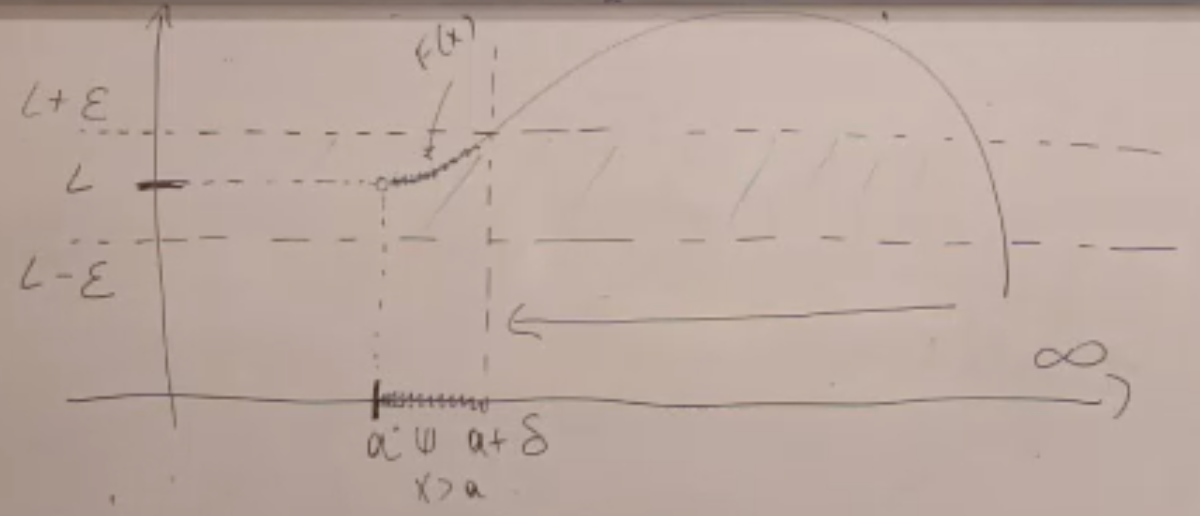
\includegraphics[scale=0.5]{rightLimit.png}
  	\centering
    \caption{right limit illustration}\label{fig:rightLimit}
\end{figure}

\newmdtheoremenv[style=defEnv]{left limit}[theorem]{Definition}
\begin{left limit}
    Let $a \in \mathbb{R}$, $F: (-\infty, a) \mapsto \mathbb{R}$, $F \rightarrow{}L \in \mathbb{R}$
    as $x \rightarrow{}a^{-}$ iff\[
        \forall \epsilon > 0, \exists \delta > 0 \,\textnormal{s.t.}\,
        x \in (a - \delta, a) \Rightarrow{}|F(x) - L| < \epsilon.
    \]
    This is called the \textbf{\emph{left-hand limit}}.
    Graphical understanding is similar to that of right limit.
\end{left limit}

\underline{Caution}: $F(a)$ does not need to be defined!

\newmdtheoremenv[style=defEnv]{left and right limit are equal}[theorem]{Lemma}
\begin{left and right limit are equal}
    Suppose $F:(a,b) \mapsto \mathbb{R}$, and assume that $\lim_{x \rightarrow{}a^{+}} = L_1$,
    $\lim_{x \rightarrow{}a^{+}} = L_2$, then $L_1 = L_2$.
\end{left and right limit are equal}

\begin{proof}
    Exercise! (Be careful to take $\delta := \min{(\delta_1, \delta_2)}$
    instead of the maximum!)
\end{proof}

\newmdtheoremenv[style=defEnv]{limit definition}[theorem]{(Limit) Definition}
\begin{limit definition}
    Let $a,L \in\mathbb{R}, f:\mathbb{R}\backslash\{a\}\mapsto\mathbb{R}$.
    $f(x)\rightarrow{}L$ as $x\rightarrow{}a$,
    or $\lim_{x\rightarrow{}a}f(x) = L$, iff\[
        \forall \epsilon>0, \exists \delta>0 \;\textnormal{s.t.}\;
        0<|x-a|<\delta \Rightarrow{}|f(x)-L|<\epsilon.
    \]
\end{limit definition}

\newmdtheoremenv[style=defEnv]{Algebra of limits}[theorem]{Definition}
\begin{Algebra of limits}
    Let $I\subset \mathbb{R}$ be an open iinterval and let $a\in I$ be a point.
    Take two functions $f,g:I\backslash\{a\}\mapsto\mathbb{R}$ s.t.\[
        \lim_{x\rightarrow{}a} f(x) = L_1 \qquad\;\textnormal{and}\;\qquad
        \lim_{x\to a} g(x) = L_2,
    \]then
    \begin{enumerate}
        \item $\lim_{a\to 0}(f(x)+g(x)) = L_1 + L_2$
        \item $\lim_{a\rightarrow{}0}(f(x)g(x)) = L_1L_2$
        \item If $f(x)\neq 0 \;\forall x$, then $\lim_{a\to{}0}\frac{1}{f(x)}=\frac{1}{L_1}$.
    \end{enumerate}
\end{Algebra of limits}

\subsection{Continuous functions}

\newmdtheoremenv[style=defEnv]{continuous at a}[theorem]{Definition}
\begin{continuous at a}
    Let $f:(b,c)\mapsto\mathbb{R}$, and pick $a\in(b,c)$.
    $f$ is \textbf{\emph{continuous at}} $a$ iff\[
        \lim_{x\rightarrow{}a}f(x) = f(a)
    \]or the other way to say it is\[
        \forall \epsilon>0, \exists \delta>0 \;\textnormal{s.t.}\;
        \forall x\in\mathbb{R}[|x-a|<\delta \Rightarrow{}|f(x) - f(a)|<\epsilon].
    \]
\end{continuous at a}

\newmdtheoremenv[style=defEnv]{continuous function}[theorem]{Definition}
\begin{continuous function}
    Let $f:I\mapsto\mathbb{R}$, where $I\subset\mathbb{R}$ is either
    \begin{itemize}
        \item an interval $(a,b)$ for some $a,b\in\mathbb{R}$, or
        \item an interval $(-\infty, b)$, or
        \item an interval $(a, \infty)$, or
        \item $I = \mathbb{R}$,
    \end{itemize}
    we say that $f$ is \textbf{\emph{continuous everywhere}}, or just \textbf{\emph{continuous}},
    if $f$ is continuous at $a \;\forall a\in I$.
    The four kinds of subsets $I\subset\mathbb{R}$ are called \textbf{\emph{open intervals}}.
\end{continuous function}

\begin{ex}
    \textbf{\emph{Rational functions}} $R(x):=\frac{P(x)}{Q(x)}$ are continuous,
    if $P, Q$ polynomial, and $Q(X) \neq 0 \;\forall x$.
\end{ex}


\paragraph{Strategy for $\epsilon-\delta$-proofs of continuity}
\begin{enumerate}
    \item Compute $f(a)$.
    \item Look at $|f(x)-f(a)|$ to see how it can be controlled by $|x-a|<\delta$.
    \item (This step may not be required.) Assume $\delta<C$ for some $C\in\mathbb{R}^{+}$
        in order to control other possible factors of $|f(x) - f(a)|$ found in the previous step.
    \item Find $\delta$ as a function of $\epsilon$ $(\delta(\epsilon))$ and write down
        the proof starting over from the begeinning.
\end{enumerate}

\newmdtheoremenv[style=defEnv]{discontinuous at a}[theorem]{Definition}
\begin{discontinuous at a}
    $f$ is \textbf{\emph{discontinuous at}} $a$ iff\[
        \exists \epsilon>0 \;\textnormal{s.t.}\; \forall\delta>0,
        \exists x\in\mathbb{R} [|x-a|<\delta \wedge|f(x)-f(a)|\ge\epsilon].
    \]
\end{discontinuous at a}

While picking the particular $x$ so that it satisfy the discontinuity condition,
ensure that it satisfy for \emph{all} $\delta$.
\begin{ex}
    $F:\mathbb{R}\rightarrow{}\mathbb{R}$,
    $g(x)=0$ when $x=0$, and $g(x) = \sin{\frac{1}{x}}$ when $x\neq 0$.
    Prove that $F$ is not continuous at 0.
\end{ex}

\newmdtheoremenv[style=defEnv]{continiuos function composition is continuous}[theorem]{Proposition}
\begin{continiuos function composition is continuous}
    Let $I \subset \mathbb{R}$ and $J \subset \mathbb{R}$ be open intervals,
    $f:I\rightarrow{}F(I)\subset J \subset\mathbb{R}$, 
    $g:J\rightarrow{}\mathbb{R}$ are continuous,
    then $g\circ f:I\rightarrow{}\mathbb{R}$ is continuous.
\end{continiuos function composition is continuous}

\subsubsection{Sequential Criterion for continuous functions}

There is connection between (convergent) sequences and continuous function.

\newmdtheoremenv[style=defEnv]{continuous function and sequences}[theorem]{Proposition}
\begin{continuous function and sequences}
    Let $I\subset \mathbb{R}$, then $f:I\rightarrow{}\mathbb{R}$ is continuous
    $\iff f(a_n) \rightarrow{} f(a)$ $\forall (a_n)$ s.t. $a_n \rightarrow{}a$.
\end{continuous function and sequences}

\begin{proof}
    Exercise!
\end{proof}

\begin{ex}
    \[
        f(x) = \left\{
            \begin{align*}
                & x^{2}, & x\in \mathbb{Q} \\
                & -x^{2}, & x\notin \mathbb{Q}
            \end{align*}
            \right. \quad\;\textnormal{if $f$ is continuous at $a$}\;.
    \]
    But $f(a_n) = a^{2}_n \rightarrow{}a^{2}$,
    $f(b_n) = -b^{2}_n \rightarrow{} -a^{2}$,
    and both are equal only if $a = 0$.
\end{ex}

\begin{ex}
    \[
        f(x) = \left\{
            \begin{align*}
                & \sin{\frac{1}{x}}, & x \neq 0 \\
                & 0, & x = 0
            \end{align*}
            \right.\quad\;\textnormal{not continuous at 0}\;.
    \]
\end{ex}

\subsubsection{continuous function on closed bounded interval}

\newmdtheoremenv[style=defEnv]{continuous for closed function}[theorem]{Definition}
\begin{continuous for closed function}
    A function $f:K\rightarrow{}\mathbb{R}$, where $K = [b,c]$, is continuous if:
    \begin{itemize}
        \item $f$ is continuous on $(b,c)$.
        \item $\lim_{x\rightarrow{}c^{-}}f(x) = f(c)$.
        \item $\lim_{x\rightarrow{}b^{+}}f(x) = f(b)$.
    \end{itemize}
\end{continuous for closed function}

\newmdtheoremenv[style=defEnv]{closed bound in open interval is continuous}[theorem]{Lemma}
\begin{closed bound in open interval is continuous}
    let $I \subset \mathbb{R}$ be open, $K \subset I$ be closed bounded.
    Then if $f:I\rightarrow{}\mathbb{R}$ continuous $\Rightarrow{}$
    $f|_K:K\rightarrow{}\mathbb{R}$ continuous.
\end{closed bound in open interval is continuous}

\newmdtheoremenv[style=defEnv]{bounded function}[theorem]{Definition}
\begin{bounded function}
    Let $S \subseteq \mathbb{R}$ be a subset, $f:S\rightarrow{}\mathbb{R}$ a function.
    $f$ is called \textbf{\emph{bounded}} $\iff$
    $\exists R\in\mathbb{R}$ s.t. $|f(x)|\le R \;\forall x \in S$.
\end{bounded function}

\underline{Warning}: Usually continuous functions on open interval are not bounded,
e.g. $\frac{1}{x}$ on $(0,1)$.

\newmdtheoremenv[style=defEnv]{sequence is bounded in closed bounded continuous func}[theorem]{Proposition}
\begin{sequence is bounded in closed bounded continuous func}
    Let $K = [b,c]$ closed bounded, $f:K\rightarrow{}\mathbb{R}$ continuous.
    Then $f$ is bounded.
\end{sequence is bounded in closed bounded continuous func}

\begin{proof}
    Assume $f$ is not bounded $\iff$
    $\forall n \in \mathbb{N}, \exists x_n \in K$ s.t. $|f(x_n)|>n$.
    Consider the sequence $(x_n)$ on $K$ $\Rightarrow{}(x_n)$ is bounded.
    By Bolzano Weierstra$\beta$, $\exists$ convergent subsequence $(x_{n_k})$
    s.t. $x_{n_k} \rightarrow{} L \in K = [b,c]$.
    Now by sequential criterion since $f$ is continuous $f(x_{n_k}) \rightarrow{}f(L)$.
    But $f$ is unbounded, therefore so is $f(x_{n_k})$, it cannot be convergent!
\end{proof}

\newmdtheoremenv[style=defEnv]{supremum of function}[theorem]{Definition}
\begin{supremum of function}
    If $S \subseteq \mathbb{R}$, $f:S\rightarrow{}\mathbb{R}$.
    $\sup{f} :=$ $ \sup{\{f(x) | x \in\ S\}}$,
    and $\inf{f}\ := \inf{\{ f(x) | x \in\ S\}}$.
\end{supremum of function}

\newmdtheoremenv[style=defEnv]{closed bounded interval func has sup}[theorem]{Theorem}
\begin{closed bounded interval func has sup}
    Let $K$ be a closed bounded interval, $f:K\rightarrow{}\mathbb{R}$ continuous. Then:
    \begin{enumerate}[label = (\arabic*)]
        \item $\exists x \in K$ s.t. $f(x) = \sup{f}$.
        \item $\exists y \in K$ s.t. $f(y) = \inf{f}$.
    \end{enumerate}
    
\end{closed bounded interval func has sup}

\begin{proof}
   \begin{enumerate}[label = (\arabic*)]
       \item Suppose that $f(x) \neq \sup{f}$, $\forall x \in K$.
           Define $g:K\rightarrow{}\mathbb{R}$, $g(x) := \frac{1}{\sup{f} - f(x)}$ well defined.
           So $g$ is continuous on a bounded interval $\Rightarrow{}$ bounded.
           Since $\sup{f}$ is supremum, $\sup{f} - \frac{1}{n}$ 
           is not an upper bound for any $n \in \mathbb{N}$.
           $\Rightarrow{} \forall n \in \mathbb{N}, \exists x_n \in K$ s.t. 
           $f(x_n) > \sup{f} - \frac{1}{n}$ $\iff$
           $\frac{1}{n}>\sup{f} - f(x_n)$ $\iff$
           $n < \frac{1}{\sup{f} - f(x_n)} = g(x_n)$ is bounded!

       \item Largely identical process of proof.
   \end{enumerate}
   
\end{proof}

\newmdtheoremenv[style=defEnv]{intermediate value theorem}[theorem]{Theorem}
\begin{intermediate value theorem}
    Let $K = [b,c]$ be a \emph{closed bounded} interval and let $f:K\rightarrow{}\mathbb{R}$
    be \emph{continuous}. Then:
    \begin{enumerate}
        \item If $f(b)\le f(c)$, let $A \in \mathbb{R}$, $f(b) \le A \le f(c)$,
            then $\exists a \in [b,c]$ s.t. $f(a) = A$
        \item If $f(b)\ge f(c)$, let $A \in \mathbb{R}$, $f(c) \le A \le f(b)$,
            then $\exists a \in [b,c]$ s.t. $f(a) = A$.
    \end{enumerate}
\end{intermediate value theorem}

\begin{proof}
    Exercise! (Hint: Use $\mathbb{R}$'s completeness axiom!)
\end{proof}

\underline{Technique}: By utilizing the $\delta$ expression,
one can always find a smaller/larger $x$ that satisfies same inequality.

\newmdtheoremenv[style=defEnv]{coro of IVT}[theorem]{Corollary}
\begin{coro of IVT}
    If $f:[b,c]\rightarrow{}\mathbb{R}$ is continuous,
    and we have $f(b) < 0$ and $f(c) < 0$ (or vice versa),
    then $\exists a \in (b,c)$ s.t. $f(a) = 0$.
\end{coro of IVT}

\newmdtheoremenv[style=defEnv]{odd degree polynomial has at least one root}[theorem]{Corollary}
\begin{odd degree polynomial has at least one root}
    Let $P:\mathbb{R}\rightarrow{}\mathbb{R}$ be any polynomial of odd degree.
    Then $P$ has at least one root.
\end{odd degree polynomial has at least one root}

\begin{proof}
    Define $P(x) = a_d x^{d} + Q(x)$, where $d \in \mathbb{N}$ is odd, $a_d\neq 0$,
    and $Q(x)$ is a polynomial of degree $\le d - 1$. 

    Proceed from here!
    (Try to connect $Q(x)$ with $a_d x^{d}$ so that e.g.\ $P(x) > 0$ when $x > 0$, and vice versa)
\end{proof}

\newmdtheoremenv[style=defEnv]{closed bounded continuous function has a fixed point}[theorem]{Corollary}
\begin{closed bounded continuous function has a fixed point}
    Let $K = [b,c]$ be a \emph{closed bounded} interval,
    $f:K\rightarrow{}K$ be a continuous function.
    Then $\exists a \in K$ s.t. $f(a) = a$.
\end{closed bounded continuous function has a fixed point}

\begin{proof}
    Exercise! (Think of a new function s.t.\ the previous corollary can be applied)
\end{proof}

\subsection{Differentiability}

\newmdtheoremenv[style=defEnv]{differentiable}[theorem]{Definition}
\begin{differentiable}
    Let $f:(b,c) \rightarrow{} \mathbb{R}, a \in (b,c)$.
    $f$ is \textbf{\emph{differentiable at $a$}} if\[
        f'(a) := \lim_{x\rightarrow{}a} \frac{f(x) - f(a)}{x - a} \;\textnormal{exists.}\;
    \]$f'(a)$ is called the \textbf{\emph{derivative}} at $a$.
\end{differentiable}

\newmdtheoremenv[style=defEnv]{differentiable alternative def}[theorem]{Definition}
\begin{differentiable alternative def}
    Let $f:(b,c) \rightarrow{} \mathbb{R}, a \in (b,c), x - a =: h$.
    $f$ is differentiable at $a$ if\[
        f'(a) := \lim_{h\rightarrow{}0} \frac{f(a + h) - f(a)}{h} \;\textnormal{exists.}\;
    \]
\end{differentiable alternative def}

\newmdtheoremenv[style=defEnv]{differentiable means continuous}[theorem]{Proposition}
\begin{differentiable means continuous}
    If $f:I\rightarrow{}\mathbb{R}$ is differentiable, $I \subset \mathbb{R}$ is open, 
    then $f$ is continuous.
\end{differentiable means continuous}

\begin{proof}
    Exercise!
\end{proof}

\underline{Warning}: The converse is not true! e.g. $f(x) = |x|$.

\newmdtheoremenv[style=defEnv]{construct secant around a}[theorem]{Proposition}
\begin{construct secant around a}
    Let $f:\mathbb{R}\rightarrow{}\mathbb{R}, I \subset \mathbb{R}$ be open, $a \in I$.
    Then the following statements are equivalent:
    \begin{itemize}
            \item $f$ is differentiable at $a$.
            \item $\exists \lambda \in \mathbb{R}, \rho:I\rightarrow{}\mathbb{R}$
            s.t. $\rho (a) = 0, \lim_{x\rightarrow{}a} \frac{\rho(x)}{x-a} = 0$, and\[
                    f(x) = f(a) + \lambda(x-a) + \rho(x).
                \]
    \end{itemize}
\end{construct secant around a}

\begin{proof}
    Exercise!
\end{proof}

\newmdtheoremenv[style=defEnv]{differentiation properties}[theorem]{Proposition}
\begin{differentiation properties}
    Let $f,g: I\rightarrow{}\mathbb{R}$ be differentiable at $a \in I$, then:
    \begin{enumerate}
        \item $f+g$ differentiable and has derivative $f'(a) + g'(a)$
        \item $fg$ differentiable and has derivative $f'(a)g(a) + f(a)g'(a)$
        \item If $f(x) \neq 0$ everywhere, then $\frac{1}{f}$ is differentiable
            with derivative $-\frac{f'(a)}{f^{2}(a)}$.
    \end{enumerate}
\end{differentiation properties}

\begin{proof}
    Exercise!
\end{proof}

\newmdtheoremenv[style=defEnv]{chain rule}[theorem]{Proposition}
\begin{chain rule}
    Let $f:I\rightarrow{}\mathbb{R}$ differentiable at $a$, 
    $g:J\subset f(I) \rightarrow{}\mathbb{R}$ differentiable at $f(a)$,
    then $g\circ f$ is differentiable at $a$, and has derivative $g'(f(a))f'(a)$.
\end{chain rule}

\begin{proof}
    Exercise!
\end{proof}

\newmdtheoremenv[style=defEnv]{inverse function differentiation}[theorem]{Proposition}
\begin{inverse function differentiation}
    Let $f:I\rightarrow{}\mathbb{R}$ \emph{strictly} increasing (or decreasing),
    differentiable at $a\in I$ s.t. $f'(a) \neq 0$.
    Then the inverse function $g:f(I)\rightarrow{}I$ exists and is differentiable with derivative\[
        g'(b) = \frac{1}{f'(a)} = \frac{1}{f'(g(b))}.
    \]
\end{inverse function differentiation}

\begin{proof}
    Exercise!
\end{proof}

\subsubsection{Extreme Values and Derivatives}

\newmdtheoremenv[style=defEnv]{global/local maximum/minimum}[theorem]{Definition}
\begin{global/local maximum/minimum}
    Let $f:I\rightarrow{}\mathbb{R}$ be a function.
    \begin{enumerate}[label = (\arabic*)]
        \item $f$ has a \textbf{\emph{global maximum}} (resp. \textbf{\emph{global minimum}})
            at $a\in I$, if $\forall x \in I, f(x) \le f(a)$ (resp. $f(x) \ge f(a)$).
        \item $f$ has a \textbf{\emph{local maximum}} (resp. \textbf{\emph{local minimum}})
            at $a\in I$ if $\exists \epsilon > 0$ s.t. $\forall x \in I \cap (a-\epsilon, a+\epsilon)$,
            $f(x) \le f(a)$ (resp. $f(x) \ge f(a)$).
    \end{enumerate}
\end{global/local maximum/minimum}

\underline{Warning}: Such values do not necessarily exists!

\newmdtheoremenv[style=defEnv]{local extremum differentiated to be 0}[theorem]{Proposition}
\begin{local extremum differentiated to be 0}
    Let $f:(b,c)\rightarrow{}\mathbb{R}$ be differentiable at $a\in(b,c)$ and 
    $f$ has a local extremum. Then $f'(a) = 0$.
\end{local extremum differentiated to be 0}

\begin{proof}
    Exercise!
\end{proof}

\underline{Warning}:
\begin{itemize}
        \item Converse is not true! e.g. $f(x) = x^{3}$.
        \item Last proposition is not true for end points!
\end{itemize}

\newmdtheoremenv[style=defEnv]{Rolle theorem}[theorem]{(Rolle) Theorem}
\begin{Rolle theorem}
    Let $f:[a,b]\rightarrow{}\mathbb{R}$ be continuous on the closed bounded interval $[a,b]$
    and differentiable on $(a,b)$. Let $f(a) = f(b)$, then $\exists x \in (a,b)$ s.t. $f'(x) = 0$.
\end{Rolle theorem}

\begin{proof}
    Exercise!
\end{proof}

\newmdtheoremenv[style=defEnv]{mean value theorem}[theorem]{(Mean Value Theorem) Theorem}
\begin{mean value theorem}
    Let $f:[a,b]\rightarrow{}\mathbb{R}$ be a continuous and differentiable on $(a,b)$.
    Then $\exists x \in (a,b)$ s.t. $f'(x) = \frac{f(b)-f(a)}{b-a}$.
\end{mean value theorem}

\begin{proof}
    Exercise! (Hint: construct a new function and apply the Rolle's Theorem.)
\end{proof}

\begin{ex}
    Show that $f(x) = 4x^{5} + x^{3} + 7x - 2$ has exactly one root.
\end{ex}

\newmdtheoremenv[style=defEnv]{strictly increasing or decreasing definition}[theorem]{Corollary}
\begin{strictly increasing or decreasing definition}
    Let $f:[a,b]\rightarrow{}\mathbb{R}$ be differentiable.
    \begin{enumerate}
        \item If $f'(x)\ge 0$ ($f'(x)>0$), then $f$ is (strictly) increasing.
        \item If $f'(x)\le 0$ ($f'(x)<0$), then $f$ is (strictly) decreasing.
    \end{enumerate}
\end{strictly increasing or decreasing definition}

\begin{proof}
    Exercise!
\end{proof}

\newmdtheoremenv[style=defEnv]{f is constant then gradient is 0}[theorem]{Corollary}
\begin{f is constant then gradient is 0}
    Let $f:[a,b]\rightarrow{}\mathbb{R}$ be continuous and differentiable on $(a,b)$.
    Then $f'(x) = 0 \;\forall x \in (a,b) \iff f$ is constant.
\end{f is constant then gradient is 0}

\underline{Technique}: Think of using MVT in ``the other way'' round: arbitrarily choose two points,
and the gradient of the line connecting the two points can be expressed using
differentiation on one point in the interval.

\newmdtheoremenv[style=defEnv]{Lipschitz continuous}[theorem]{Proposition}
\begin{Lipschitz continuous}
    Let $f:I\rightarrow{}\mathbb{R}$ be differentiable.
    Let $L\in \mathbb{R}^{+}$ s.t. $|f'(x)|\le L \;\forall x \in I$.
    Then $\forall x_1, x_2\in I$,\[
        |f(x_1) - f(x_2)| \le L|x_1 - x_2|.
    \]
    A function satisfying the above inequality is called \textbf{\emph{Lipschitz continuous}}.
\end{Lipschitz continuous}








% End of Analysis


\end{document}%chktex 7, chktex 17
